%input macros (i.e. write your own macros file called MacroFile1.tex)
%\include{Macros/MacroFile1}

\documentclass[oneside,a4paper,12pt,times,openright]{Classes/CUEDthesisPSnPDF}
%\usepackage[margin=1in]{geometry}
\usepackage{graphicx}
\usepackage{xcolor}
\usepackage{wrapfig}
\usepackage{helvet}
%\usepackage{fullpage}
\usepackage{amsmath}
\usepackage{subfig}
\usepackage{setspace}
\usepackage{tocbibind}
\usepackage{anysize}
\usepackage{fancyhdr}
\usepackage[Lenny]{fncychap}
\usepackage[T1]{fontenc}
\usepackage{fouriernc}
\usepackage{amssymb}
\usepackage{amsfonts}
\usepackage{latexsym}
\setcounter{secnumdepth}{5}
\setcounter{tocdepth}{2}
\usepackage{multirow}
%\usepackage{appendix}
\usepackage[inner=3.75cm,outer=3cm]{geometry}
\usepackage{multicol}

\usepackage{hyphenat}

%\usepackage[square, sort, numbers, authoryear]{natbib}
\usepackage[square, sort&compress, numbers]{natbib}

\usepackage{lipsum}
\usepackage{diagbox}
\usepackage{booktabs}
\usepackage{multirow}
\usepackage{multicol}
\usepackage{tabularx}
%\usepackage{algorithm}
%\usepackage{algorithmic}
\usepackage{algorithm2e}
\usepackage[noend]{algpseudocode}
\usepackage[standard]{ntheorem}

\usepackage{enumerate}
\usepackage{array}
\usepackage{url}
%\usepackage{cite}
%\usepackage[symbol]{footmisc}
%\usepackage{subcaption}
\usepackage{nomencl}

\newcommand{\newappendix}{%
	\refstepcounter{chapter}\chapter*{Appendix \thechapter}%
	\addcontentsline{toc}{chapter}{Appendix \thechapter}%
}


\makenomenclature

%\linespread{2}
\renewcommand{\baselinestretch}{2}

%\marginsize{3cm}{2cm}{3cm}{2cm}

\ifpdf
    \pdfinfo { /Title  (DoctoralThesis)
               /Author (Pallab Maji, pallab.vsp@gmail.com)
               /CreationDate (D:20110512000000)  %format D:YYYYMMDDhhmmss
               /ModDate (D:20110601213532)
               /Subject (Writing a Master's thesis)
               /Keywords (M.Tech, Thesis)}
    \pdfcatalog { /PageMode (/UseOutlines)
                  /OpenAction (fitbh)  }
\fi


%------------------My Publication_------------------

%\DeclareBibliographyOption{biblabel}{%
%	\ifstrequal{#1}{brackets}
%	{%
%		\DeclareFieldFormat{labelnumberwidth}{\mkbibbrackets{##1}}%
%		\setlength{\biblabelsep}{10 pt}%
%	}
%	{%
%		\DeclareFieldFormat{labelnumberwidth}{\mkbibsuperscript{##1}}%
%		\setlength{\biblabelsep}{0 pt}%
%	}%
%}

%---------------------END-------------------------------




% turn of those nasty overfull and underfull hboxes
\hbadness=10000
\hfuzz=50pt

% Put all the style files you want in the directory StyleFiles and usepackage like this:
\usepackage{StyleFiles/watermark}

% Comment out the next line to get single spacing
\onehalfspacing

\hyphenation{op-tical net-works semi-conduc-tor}

\begin{document}

%\language{english}

% A page with the abstract on including title and author etc may be
% required to be handed in separately. If this is not so, then comment
% the below 3 lines (between '\begin{abstractseparte}' and
% 'end{abstractseparate}'), normally like a declaration ... needs some more
% work, mind as environment abstracts creates a new page!
% \begin{abstractseparate}
%   
% Thesis Abstract -----------------------------------------------------


%\begin{abstractslong}    %uncommenting this line, gives a different abstract heading
\begin{abstracts}        %this creates the heading for the abstract page
	
	Soft computing techniques, unlike traditional deterministic logic based computing techniques, sometimes also called as hard computing, are tolerant of imprecision, uncertainty, and approximation. The primary inspiration for soft computing is the human mind and its ability to address day-to-day problems. The primary constituents of soft computing techniques are Artificial Neural Network, Fuzzy Logic Systems, and Evolutionary Computing.
	
	This thesis presents design and implementation of a generic hardware architecture based Type-I Mamdani fuzzy logic controller (FLC) implemented on a programmable device, which can be remotely configured in real-time over Ethernet. This reconfigurability is added as a feature to existing FLCs in literature. It enables users to change parameters (those drive the FLC systems) in real-time and eliminate repeated hardware programming whenever there is a need. Realization of these systems in real-time is  difficult as the computational complexity increases exponentially with an increase in the number of inputs. Hence challenge lies in reducing the Rulebase significantly such that the inference time and the throughput time is perceivable for real-time applications.
	
	To achieve these objectives, a modified thresholded fired rules hypercube (MT-FRHC) algorithm for Rulebase reduction is proposed and implemented. MT-FRHC reduces the useful rules without compromising system accuracy and improves the cycle time in terms of fuzzy logic operations per second (FzLOPS). It is imperative to understand that there are over sixty reconfigurable parameters, and it becomes an arduous task for a user to manage them. Therefore, a genetic algorithm based parameter extraction technique is proposed. This will help to develop a course tuning and provide default parameters that can be later fine tuned by the users remotely through the Web-based User Interface. A hardware software co-design architecture for FLC is developed on TI C6748 DSP hardware with Sys/BIOS RTOS and seamlessly integrated with a web-based user interface (WebUI) for reconfigurability.
	
	Fuzzy systems employ defuzzifier to convert the fuzzy output into the real world crisp output. Centroid of Area (CoA) method is most widely used defuzzification method for control applications. However, the prevalent method of CoA computation is based on the principle of Riemann sum which is computationally complex. A vertices based CoA (VBCoA) defuzzification method is introduced. It has been observed that the proposed VBCoA method for COA computation is faster than the Riemann sum based CoA computation.
	
	A code optimization technique, exclusive to TI DSPs, is implemented to achieve memory and machine cycle optimization. The WebUI is developed in accordance to a client--server model using ASP.NET. It acquires fuzzy parameters from users, and a server application is dedicated to handling data communication between the hardware and the server. Testing and analysis of this hardware G-FLCS has been carried out by using hardware-in-loop test to control various system models in Simulink environment which includes water level control in a two tank system, intelligent cruise control system, speed control of an armature controlled DC motor and anti-windup control. The performance of the proposed G-FLCS is compared to Fuzzy Inference System of Matlab Fuzzy Logic Toolbox and PID controller in terms of settling time, transient time and steady state error. This proposed MT-FRHC based G-FLCS with VBCoA defuzzification implemented on C6748 DSP was finally deployed to control the radial position of plasma in Aditya Tokamak fusion reactor. The proposed G-FLCS is observed to deliver a smooth and fast system response.
	
\end{abstracts}
%\end{abstractlongs}


% ----------------------------------------------------------------------


%%% Local Variables:
%%% mode: latex
%%% TeX-master: "../thesis"
%%% End:

% \end{abstractseparate}

%------------------------------------------
%         Cover page
%------------------------------------------
\begin{titlepage}


\noindent{\LARGE \textbf{{On Design and Implementation of Generic \\\tiny~\\ \LARGE Fuzzy Logic Controllers}}}
\par

\vspace{3.2in}
\noindent{\Large Pallab Maji}
%{\small by\\~\\\Large Pallab Maji}
\vspace{3.2in}
\\

%\noindent
\includegraphics[scale=0.3]{logo}\\[0.1in]
%\par
%%------------------------------------
%%         END FIGURE
%
%\vspace{0.2in}
%\noindent\large Dept. Electronics and Communication Engineering\\
%\noindent National Institute of Technology, Rourkela\\Orissa-769008, India\\
%\vspace{0.1in}

\begin{minipage}{.1\linewidth}
	\hspace*{-.6cm}
\includegraphics[height=2.2cm]{logo}
\end{minipage}
\hspace{.2cm}
\begin{minipage}{.9\linewidth}
	%\begin{flushleft}
	{\large
		{\textbf{Dept. of Electronics \& Communication Engineering}\\
			\textbf{National Institute of Technology Rourkela\\}}}
	{\large
		{Rourkela, Odisha, India-769 008}}
	
	%\end{flushleft}
\end{minipage}

\end{titlepage}

%\begin{titlepage}

\noindent{\LARGE \textbf{{\textcolor{blue}{On Design and Implementation of Generic \\\tiny~\\ \LARGE Fuzzy Logic Controllers}}}}
\par
\vspace{3.2in}
\noindent{\LARGE \textcolor{blue}{Pallab Maji}}
%{\small by\\~\\\Large Pallab Maji}
\vspace{3.2in}
\\

\begin{minipage}{.1\linewidth}
	\hspace*{-.6cm}
\includegraphics[height=2.2cm]{cover/logo_blue}
\end{minipage}
\hspace{.2cm}
\begin{minipage}{.9\linewidth}
	%\begin{flushleft}
	\textcolor{blue}{
	{\large
		{\textbf{Dept. of Electronics \& Communication Engineering}\\
			\textbf{National Institute of Technology Rourkela\\}}}
	{\large
		{Rourkela, Odisha, India-769 008}}}
	
	%\end{flushleft}
\end{minipage}

\end{titlepage}

%------------------------------------------
%         Cover Page Completed
%------------------------------------------

%   TITLE PAGE
%------------------------------------------
\begin{titlepage}
\begin{center}

{\LARGE {On Design and Implementation of Generic \\\tiny~\\ \LARGE Fuzzy Logic Controllers}}
\par
\vspace{.4in}
\small{\textit{Thesis submitted for partial fulfilment of the\\requirements for the degree of}\\ \vspace{0.2in} \large{Doctor of Philosophy}}
\\\textit{in}\\\large Electronics and Communication Engineering\\
\par
{\small by\\~\\\Large Pallab Maji\\\small (Roll No.: 511EC604)}
%{\small by\\~\\\Large Pallab Maji}
\vspace{0.2in}
\\
\small \textit{Under the Supervision of} \\
	\vspace{0.1in}
	\large Prof. Sarat Kumar Patra \\ 
	\small \textit{and} \\
	\large Prof. Kamalakanta Mahapatra \\
	\vspace{0.9in}

\includegraphics[scale=0.3]{logo}\\[0.1in]
\par
%------------------------------------
%         END FIGURE


\large Dept. Electronics and Communication Engineering\\
National Institute of Technology, Rourkela\\Orissa-769008, India\\
\vspace{0.1in}
June, 2015
\end{center}
\end{titlepage}


%------------END of TITLE PAGE-----------------------------------



% Using the watermark package which is in StyleFiles/
% and to remove DRAFT COPY ONLY appearing on the top of all pages comment out below line
%\watermark{DRAFT COPY ONLY}




%set the number of sectioning levels that get number and appear in the contents


\frontmatter % book mode only
\pagenumbering{roman}
\thispagestyle{empty}

\begin{minipage}{.1\linewidth}
\hspace*{-.6cm}
\includegraphics[height=2.2cm]{logo}
\end{minipage}
\hspace{.2cm}
\begin{minipage}{.9\linewidth}
%\begin{flushleft}
{\large
{\textbf{Dept. of Electronics \& Communication Engineering}\\
\textbf{National Institute of Technology Rourkela\\}}}
{\large
{Rourkela, Odisha, India-769 008}}

%\end{flushleft}
\end{minipage}
\vskip .2cm
\hrule
%\vspace{0.5in}
%\vfill
\vskip 1cm

\begin{flushright}
{June 24, 2015}
\end{flushright}



\vspace{0.5in}

\centerline{\Large{\bf Certificate}}
\vspace{1cm}
%\fontsize{14pt}{16.8pt}
%\begin{large}
\noindent
This is to certify that the work in the thesis entitled {\bf \emph{``On Design and Implementation of Generic Fuzzy Logic Controllers''}} by {\bf {Pallab Maji}} is a record of an original research work carried out under our supervision and guidance in partial fulfillment of the requirements for the award of the degree of Doctor of Philosophy in Electronics and Communication Engineering. Neither this thesis nor any part of it has been submitted for any degree or academic award elsewhere.\\
%\end{large}
%\vspace{1.1in}
%\noindent
%\linespread{1}
%\begin{table}[h!]
%%\centering
%\begin{tabular}{ l  l }
%
%%{\includegraphics[width = 60pt]{PGbw_1}}&&%{\includegraphics[width = 60pt]{bm.eps}}
%%\\
%{\bf Prof. Ganapati Panda}                 & $\qquad \;\qquad \;${\bf Prof. Bernard Mulgrew} \\
%\fontsize{10}{1} \selectfont
%$\!\!$Professor                                  & $\qquad \qquad$ \fontsize{10}{1} \selectfont Professor\\
%\fontsize{10}{1} \selectfont $\!\!$School of Electrical Sciences              &$\qquad \qquad$ \fontsize{10}{1} \selectfont Institute for Digital Communication\\
%\fontsize{10}{1} \selectfont $\!\!$Indian Institute of Technology Bhubaneswar &$\qquad \qquad$ \fontsize{10}{1} \selectfont The University of Edinburgh\\
%\fontsize{10}{1} \selectfont $\!\!$Odisha, India - 751 013                     &$\qquad \qquad$ \fontsize{10}{1} \selectfont Scotland, UK
%\end{tabular}
%\end{table}
%%\fontsize{12pt}{14.4pt}
\vskip 2cm
%\vspace{smallskipamount}
%\hskip .45\textwidth \begin{minipage}[b]{7.5cm}
%\onehalfspacing
%Dr. Samit Ari\\
%\\ Assistant Professor \\
%
% Prof. Sarat Kumar Patra \\
% \\
%  Professor \& Dean (FA) \\
%  \\
%  Dept. of Electronics \& Comm. Engg. \\
%  \\
% National Institute of Technology, Rourkela \\
% \\
%  India,Odisha-769008 \\
%  \end{minipage}
\vspace{1cm}

\begin{table}[htbp]
  \centering
  %\caption{Description of different waves and segments in a ECG cycle}
%  \begin{tabular}{p{8cm}  p{8cm}}
\begin{tabular}{>{\centering\arraybackslash}p{6.5cm} >{\centering\arraybackslash}p{8.5cm}}
  \textbf{Dr. Kamalakanta Mahapatra}  & \textbf{Dr. Sarat Kumar Patra}  \\
   (Co-Supervisor) & (Supervisor) \\
  Professor, Dept. of ECE &  Professor, Dept. of ECE \\
  %ECE Department & ECE Department\\
  NIT Rourkela, Odisha & NIT Rourkela, Odisha\\

 %Dept. of Electronics \& Comm. Engg. &Dept. of Electronics \& Comm. Engg.\\
% National Institute of Technology, Rourkela & National Institute of Technology, Rourkela\\
%India,Odisha-769008 & India,Odisha-769008 \\


%\end{minipage}
%& Dr. Samit Ari\\
%\\
%& Assistant Professor\\
%\\
%& Dept. of Electronics \& Comm. Engg.\\
%\\
%& National Institute of Technology, Rourkela\\
%\\
%& India,Odisha-769008 \\

  \end{tabular}%
 % \label{tab:addlabel}%
\end{table}% 
% Thesis Dedictation ---------------------------------------------------

\begin{dedication} %this creates the heading for the dedication page

Dedicated\\to\\my family....


\end{dedication}

% ----------------------------------------------------------------------

%%% Local Variables:
%%% mode: latex
%%% TeX-master: "../thesis"
%%% End:

\begin{declaration}

I certify that
\vspace{1cm}
\begin{enumerate}[(a)]
	\item The work contained in this thesis is original and has been done by me under the guidance of my supervisors.
	\item The work has not been submitted to any other Institute for any degree or diploma.
	\item I have followed the guidelines provided by the Institute in preparing the thesis.
	\item I have conformed to the norms and guidelines given in the Ethical Code of Conduct of the Institute.
	\item Whenever I have used materials (data, theoretical analysis, figures, and text) from other sources, I have given due credit to them by citing them in the text of the thesis and giving their details in the references. Further, I have taken permission from the copyright owners of the sources, whenever necessary.
\end{enumerate}

\vspace{1cm}
\begin{flushright}
	\large Pallab Maji\\
	\ %small\textit{pallab.vsp@gmail.com}
\end{flushright}

\end{declaration}
% Thesis Acknowledgements ------------------------------------------------


%\begin{acknowledgementslong} %uncommenting this line, gives a different acknowledgements heading
\begin{acknowledgements}      %this creates the heading for the acknowlegments


This dissertation would not have been possible without the guidance and the help of several individuals who in one way or another contributed and extended their valuable assistance in course of this study.

\vspace{.5cm}
The author would like to thank his supervisor, Dr. Sarat Kumar Patra, for his guidance and support on this research work. The author would also like to acknowledge his co-supervisor, Dr. Kamalakanta Mahapatra for his kind advice and inspiration. 

\vspace{.5cm}
The author would like to thank Board of Research for Fusion Science and Technology (BRFST) and Institute of Plasma Research, Gandhinagar for funding major part of this research. The author would like to extend his gratitude towards Dr. Govindarajan, Mr. J. J. Patel, Mrs. Rachana Rajpal and Mr. Hitesh Patel of Institute of Plasma Research, Gandhinagar, for their contributions to this project. 

\vspace{.5cm}
The author would also like to thank Prof. B. Subudhi, Prof. D. P. Acharya, Prof. P. M. Khillar and Prof. S. Meher for their innovative ideas and review during the entire duration of the project. 

\vspace{.5cm}
The author would also like to acknowledge and appreciate the help from the faculty members especially Prof. S. Hiremath, Prof. A. K. Swain, Prof. M. Okhade and Prof. S. Deshmukh of the department for their continuous encouragement to delve into analytical aspects of this work. The author would be grateful to the support extended by the staff members of the department, specially Mr. P. Oram and Mr. Ishwar during the entire journey.

\vspace{.5cm}
The author would also like to thank his friends, especially Deepak, Umakant, Bodhisattwa, Bhaskar, Chithra, Manas, Varun, Goutam, Sankat, Bibhu, Deepak, Asis and Pramit for their accompaniment. Their enduring effort in proof reading of the thesis is unforgettable. The author would also like to extend his gratitude to his seniors Prashant, Sudheendra, Jagannath, Yogesh, Manab and Dipak. The author would also like to thank his lab partner Satyendra for his extensive support and assistance during the entire period of his doctoral studies.

\vspace{.5cm}
And finally the author would like to thank his family and friends, whose faith and patience had always been the inspiring factor.

\vspace{1cm}
\begin{flushright}
\large Pallab Maji\\
\small\textit{pallab.vsp@gmail.com}
\end{flushright}


\end{acknowledgements}
%\end{acknowledgmentslong}

% ------------------------------------------------------------------------

%%% Local Variables:
%%% mode: latex
%%% TeX-master: "../thesis"
%%% End:


% Thesis Abstract -----------------------------------------------------


%\begin{abstractslong}    %uncommenting this line, gives a different abstract heading
\begin{abstracts}        %this creates the heading for the abstract page
	
	Soft computing techniques, unlike traditional deterministic logic based computing techniques, sometimes also called as hard computing, are tolerant of imprecision, uncertainty, and approximation. The primary inspiration for soft computing is the human mind and its ability to address day-to-day problems. The primary constituents of soft computing techniques are Artificial Neural Network, Fuzzy Logic Systems, and Evolutionary Computing.
	
	This thesis presents design and implementation of a generic hardware architecture based Type-I Mamdani fuzzy logic controller (FLC) implemented on a programmable device, which can be remotely configured in real-time over Ethernet. This reconfigurability is added as a feature to existing FLCs in literature. It enables users to change parameters (those drive the FLC systems) in real-time and eliminate repeated hardware programming whenever there is a need. Realization of these systems in real-time is  difficult as the computational complexity increases exponentially with an increase in the number of inputs. Hence challenge lies in reducing the Rulebase significantly such that the inference time and the throughput time is perceivable for real-time applications.
	
	To achieve these objectives, a modified thresholded fired rules hypercube (MT-FRHC) algorithm for Rulebase reduction is proposed and implemented. MT-FRHC reduces the useful rules without compromising system accuracy and improves the cycle time in terms of fuzzy logic operations per second (FzLOPS). It is imperative to understand that there are over sixty reconfigurable parameters, and it becomes an arduous task for a user to manage them. Therefore, a genetic algorithm based parameter extraction technique is proposed. This will help to develop a course tuning and provide default parameters that can be later fine tuned by the users remotely through the Web-based User Interface. A hardware software co-design architecture for FLC is developed on TI C6748 DSP hardware with Sys/BIOS RTOS and seamlessly integrated with a web-based user interface (WebUI) for reconfigurability.
	
	Fuzzy systems employ defuzzifier to convert the fuzzy output into the real world crisp output. Centroid of Area (CoA) method is most widely used defuzzification method for control applications. However, the prevalent method of CoA computation is based on the principle of Riemann sum which is computationally complex. A vertices based CoA (VBCoA) defuzzification method is introduced. It has been observed that the proposed VBCoA method for COA computation is faster than the Riemann sum based CoA computation.
	
	A code optimization technique, exclusive to TI DSPs, is implemented to achieve memory and machine cycle optimization. The WebUI is developed in accordance to a client--server model using ASP.NET. It acquires fuzzy parameters from users, and a server application is dedicated to handling data communication between the hardware and the server. Testing and analysis of this hardware G-FLCS has been carried out by using hardware-in-loop test to control various system models in Simulink environment which includes water level control in a two tank system, intelligent cruise control system, speed control of an armature controlled DC motor and anti-windup control. The performance of the proposed G-FLCS is compared to Fuzzy Inference System of Matlab Fuzzy Logic Toolbox and PID controller in terms of settling time, transient time and steady state error. This proposed MT-FRHC based G-FLCS with VBCoA defuzzification implemented on C6748 DSP was finally deployed to control the radial position of plasma in Aditya Tokamak fusion reactor. The proposed G-FLCS is observed to deliver a smooth and fast system response.
	
\end{abstracts}
%\end{abstractlongs}


% ----------------------------------------------------------------------


%%% Local Variables:
%%% mode: latex
%%% TeX-master: "../thesis"
%%% End:


\headsep = 25pt
\pagestyle{fancy}
\fancyhf{}

%\fancyhead[R]{\slshape \rightmark}
\fancyhead[R]{\slshape \nouppercase \rightmark}    %Remove no \nouppercase for Capitalization
%\fancyhead[LO,RE]{\slshape \thechapter}
\fancyfoot[C]{\thepage}

\tableofcontents
\listoffigures
\listoftables
\chapter{List of Symbols}

\begin{table}[ht]
	\centering
	\begin{tabular}{l l p{10cm}}
		$\Delta $ & ~ & Fuzzy operator \\
		$\Delta ^{-1}$ & ~ & Inverse fuzzy operator \\
		$\Lambda_c$ & ~ & Digital to Analog Converter \\
		$'$ & ~ & Matrix or vector transpose \\
		$\bigcap {} $ & ~ & T-norm operator. Basic operation includes Minimum, Product, Lukasiewicz, etc. Operated on a vector \\
		$ \bigcup {} $ & ~ & T-conorm operator. Basic operation includes Maximum, Product, Lukasiewicz, etc \\
		$ \mathcal{O} $ & ~ & \emph{Big O} notation for complexity \\
		$ \overrightarrow {X(i)} $ & ~ &  implies a vector formed from $ i^{th} $ row of matrix $ X $ \\
		$\to$ & ~ & implies in between \\
		$ \mu $ & ~ & Membership function \\
		$ \mu\left( x\right) $ & ~ & Value of Membership function for real value $x$ \\
		\textbf{B} & ~ & Magnetic flux density \\
		$ B_\phi, B_\theta, B_\rho $ & ~ & Toroidal, poloidal and radial components of the magnetic field\\
		$E$ & ~ & Electric field intensity\\
		$ J $ & ~ & Plasma current density\\
		$ R $ & ~ & Major radial coordinate\\
		$ a $ & ~ & Minor radial coordinate\\
		$\Gamma $ & ~ & Shafranov parameter \\
		~ & ~ & ~
	\end{tabular}
\end{table}
\chapter{List of Acronyms}

\begin{table}[ht]
	\centering
	\begin{tabular}{l l l}
		AC & ~ & Alternating Current \\
		ACDC & ~ & Armature Control Direct Current \\
		ADC & ~ & Analog to Digital Converter \\
		ASIC & ~ & Application Specific Integrated Circuit \\
		ASIP & ~ & Application Specific Integrated Processor \\
		ASP & ~ & Active Server Pages \\
		BOA & ~ & Bisector of Area \\
		CAN & ~ & Controller Area Network \\
		CMOS & ~ & Complementary Metal Oxide Semiconductor \\
		COA & ~ & Centroid of Area \\
		COG & ~ & Center of Gravity \\
		DAC & ~ & Digital to Analog Converter \\
		DC & ~ & Direct Current \\
		DSP & ~ & Digital Signal Processor \\
		FIS & ~ & Fuzzy Inference System \\
		FLC & ~ & Fuzzy Logic Controller \\
		FCP & ~ & Fuzzy Control Parameters \\
		FLIPS & ~ & Fuzzy Logic Inferences Per Second \\
		FPGA & ~ & Field Programmable Gate Array \\
		FzLOPS & ~ & Fuzzy Logic Operations Per Second \\
		IIS & ~ & Internet Information Server \\
		IC & ~ & Integrated Circuits \\
		LAN & ~ & Local Area Network \\
		LOM & ~ & Largest of Maximum \\
		MF & ~ & Membership Function \\
		MFG & ~ & Membership Function Generator \\
		MFRPS & ~ & Mega Fuzzy Rules Per Second \\
		MOM & ~ & Middle of Maximum \\
		OMP & ~ & Overlapping Membership Function
	\end{tabular}
\end{table}

\makeatletter
\setlength{\@fptop}{0pt}
\makeatother

\begin{table}[t!]
	\centering
	\begin{tabular}{l l l}
		PID & ~ & Proportional Integral Derivative \\
		SOM & ~ & Smallest of Maximum \\
		SPI & ~ & Serial Peripheral Interface \\
		SIMD & ~ & Single Instruction Multiple Data \\
		TCP & ~ & Transmission Control Protocol \\
		TI & ~ & Texas Instruments \\
		UART & ~ & Universal Asynchronous Receiver and Transmitter\\
		VLIW & ~ & Very Long Instruction Word
		
	\end{tabular}
\end{table}


\lstlistoflistings		% List of Code Snippets
%\printnomenclature  %% Print the nomenclature
%\addcontentsline{toc}{chapter}{Nomenclature}



\mainmatter % book mode only
\chapter{Introduction}
\begin{chapterAbstract}{Overview}
	This chapter presents the fundamental concepts of a fuzzy system. It reviews few of the existing fuzzy logic controller designs reported in the literature and analyzes their implementation techniques. This chapter also address the issues of reconfigurability and generality of the existing fuzzy system designs, thereby lay the foundation of this research work and its contribution. 
	
\end{chapterAbstract}
\clearpage
~\\
``We human beings, live in a very imprecise world. A world where our perception of reality are far more important than actual reality.''

\noindent{\bfseries\large\hfill Daniel Keys Moran}
\\
~\\
~\par
It is well known that a human mind efficiently utilizes the modes of imprecision and uncertainty to solve everyday problems. It is this tolerance of imprecision, uncertainty, and approximation that helps human being make informative decisions and enforce reasoning with ease and in a short time. It is true that precision and certainty has ensured that mankind is able to fire precision laser over a long distance, build powerful processors with trillions of transistors, developed terra\hyp{}pixel imaging devices, focus microscopic beams of electron to capture minute details in nanometer scale, and accomplish many more unimaginable achievement in science and technology. However, requiring precision in engineering problems incurs a high cost and long lead time in development. Prof. Lotfi Askar Zadeh described the power of uncertainty and approximate reasoning over hard computing by illustrating how a human mind work while \textit{parking a vehicle}\cite{Zadeh1993}. T. Ross took the instance of \textit{traveling salesman} problem to exemplify similar point \cite{Ross2010}. It is, therefore, important for any scientist or engineer to contemplate the requirement for approximate reasoning and imprecision while considering fuzzy logic to solve a problem. The prime desideratum is {``how much imprecision can the system tolerate''}.

\section{Introduction to Fuzzy Logic Systems}

Lotfi Askar Zadeh in 1965 \cite{zadeh1965fuzzy} proposed fuzzy sets and described it as ``a class of objects with a continuum of grades of membership. Such a set is characterized by a membership function that assigns to each object a grade of membership ranging from zero to one.'' All fuzzy logic systems operate on this principle to mathematically represent linguistic variables and heuristic knowledge. Fuzzy logic systems provide an alternative to the predominant conventional binary and deterministic logic based crisp data processing systems. Fuzzy set theory provides the mathematical tool to carry out approximate reasoning and to handle imprecision or vagueness of information. The concept of degrees of membership is employed to provide a mathematical definition of fuzzy sets. This enables various circumstances encountered in human reasoning to objectify into scientific form.

\section{Fuzzy Sets}
Conventional bivalent set theory, often known as conventional set theory,  can be limiting in describing a 'humanistic' problem mathematically. For example, Fig. \ref{fig:Fig4_b_set} below illustrates bivalent sets to model room temperature. It is obvious that the limiting feature of conventional sets is that they are mutually exclusive.
\begin{figure}[h]
\centering
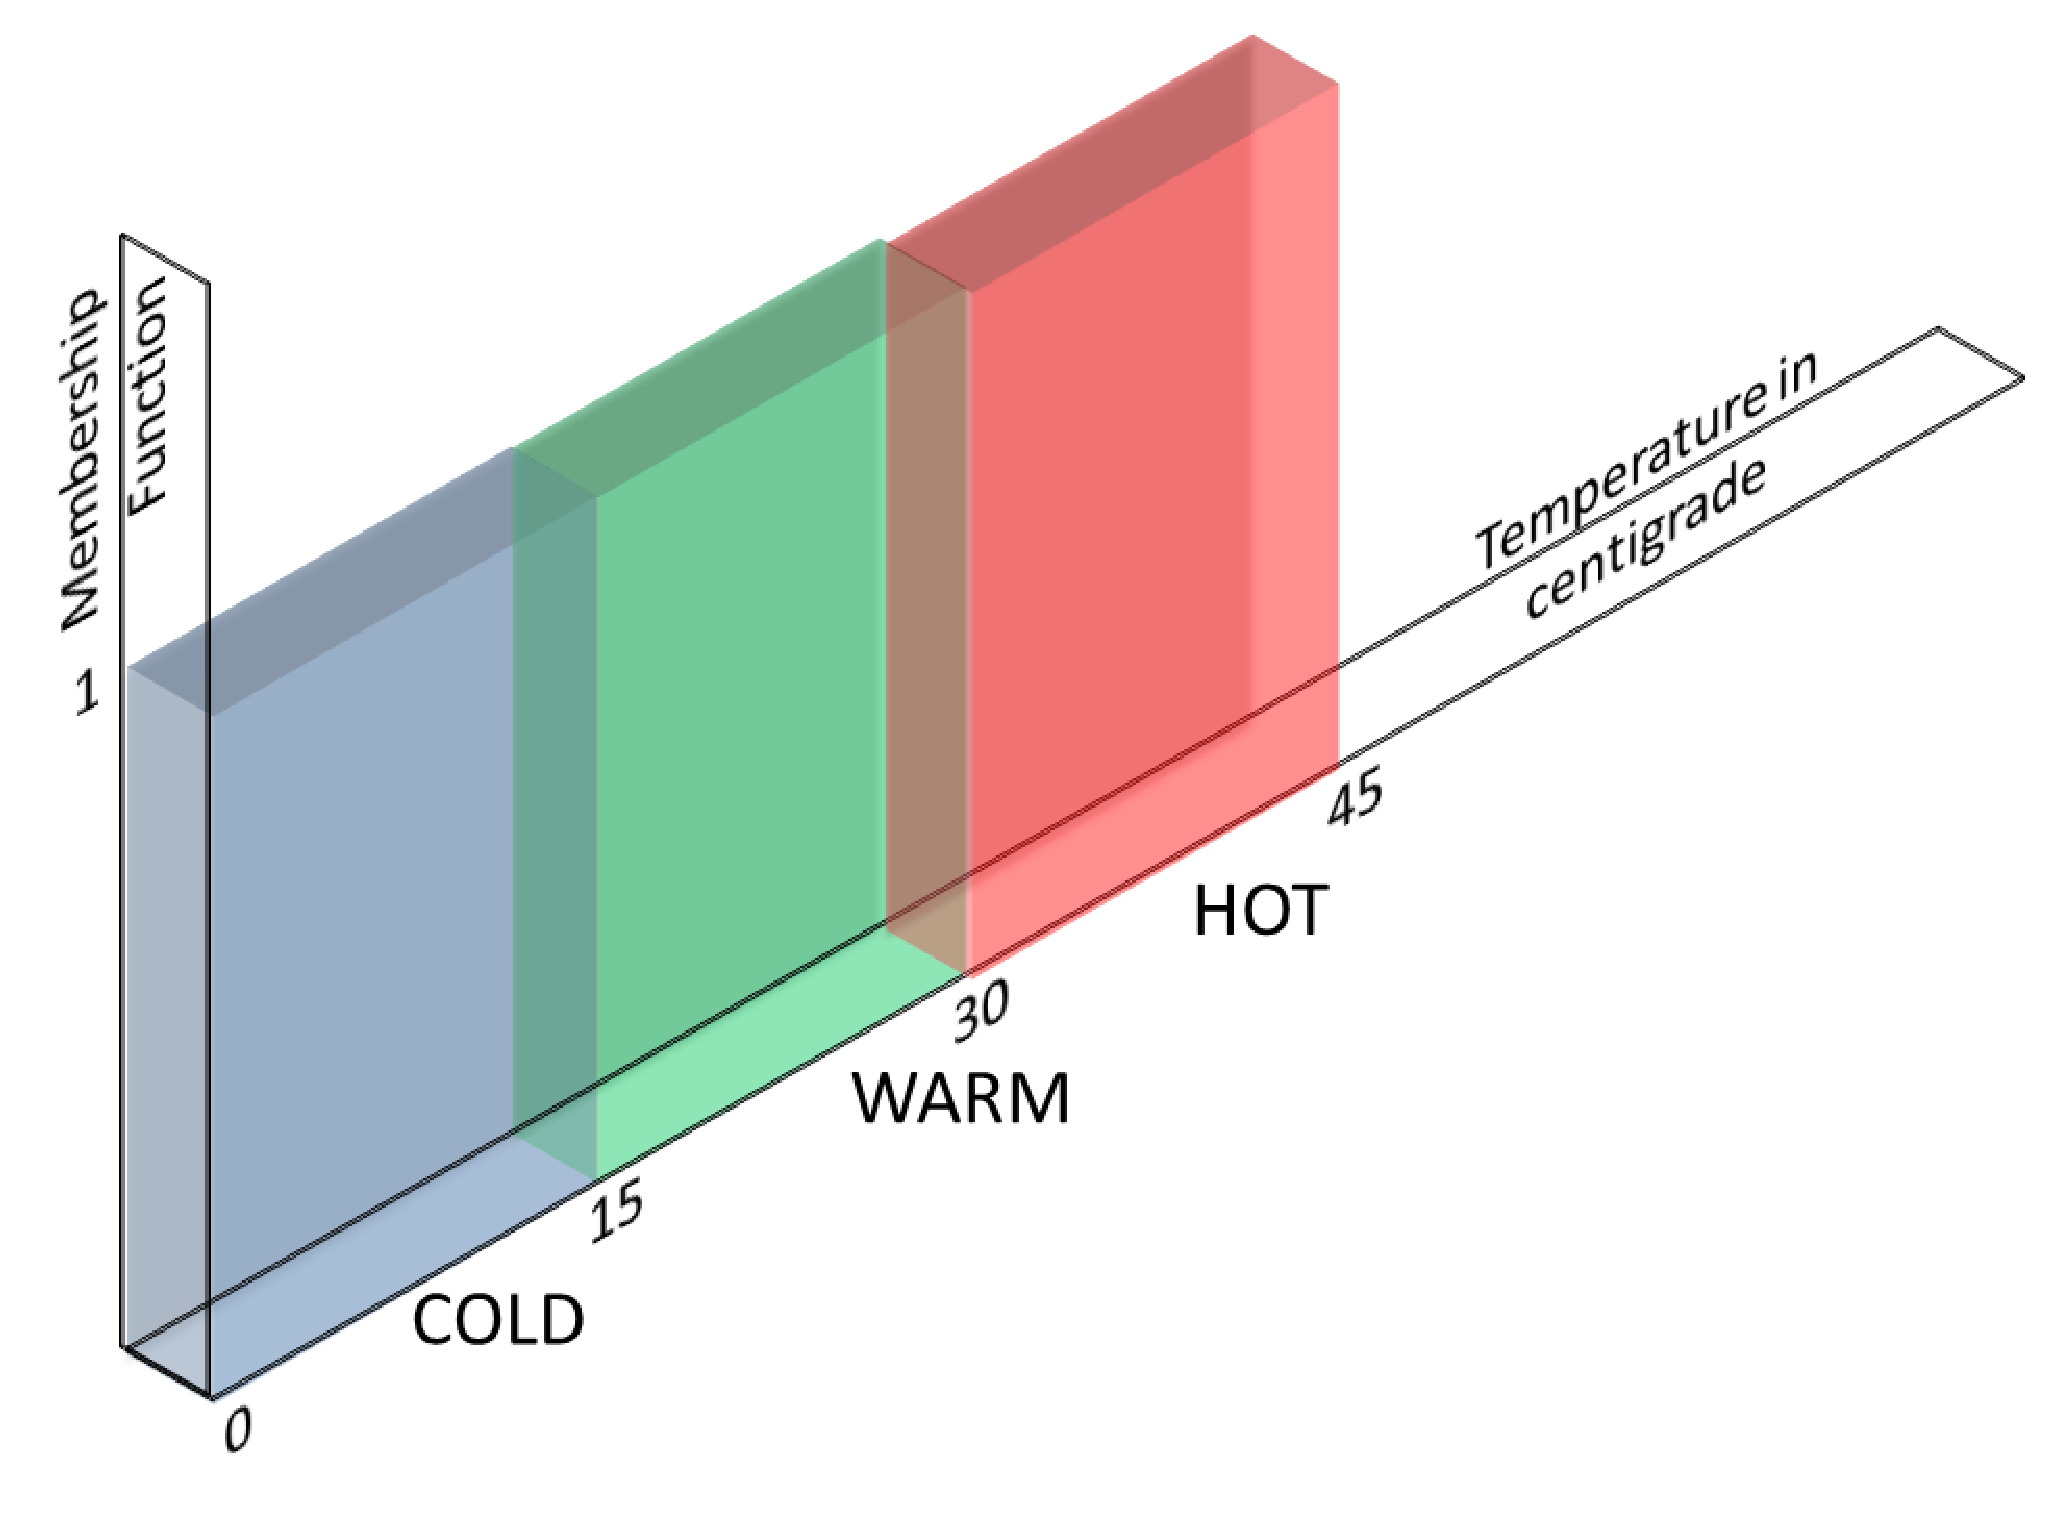
\includegraphics[width=0.8\linewidth]{Chapter1/chapter1/Fig4_b_set}
\caption{Bivalent sets to model room temperature.}
\label{fig:Fig4_b_set}
\end{figure}

 It becomes impossible to generate association  of a variable to more than one set. Based on how human achieves perception, it is inaccurate to model transition from quantity `\textbf{cool}' to `\textbf{warm}' when one degree centigrade of heat is added to the system. The actual modeling in real life however, occurs with a smooth transition or drift from `\textbf{cool}' to `\textbf{warm}'. This transition can be captured if the association itself can be modeled using some functions as depicted in Fig. \ref{fig:Fig5_f_set}. Here, the association is modeled as a triangular function. In fuzzy logic theory, the function which defines the association is called as membership function. Thereby, in fuzzy set theory, apart from the value of the variable, the degree of association of the variable to the set is also captured.
\begin{figure}[h]
\centering
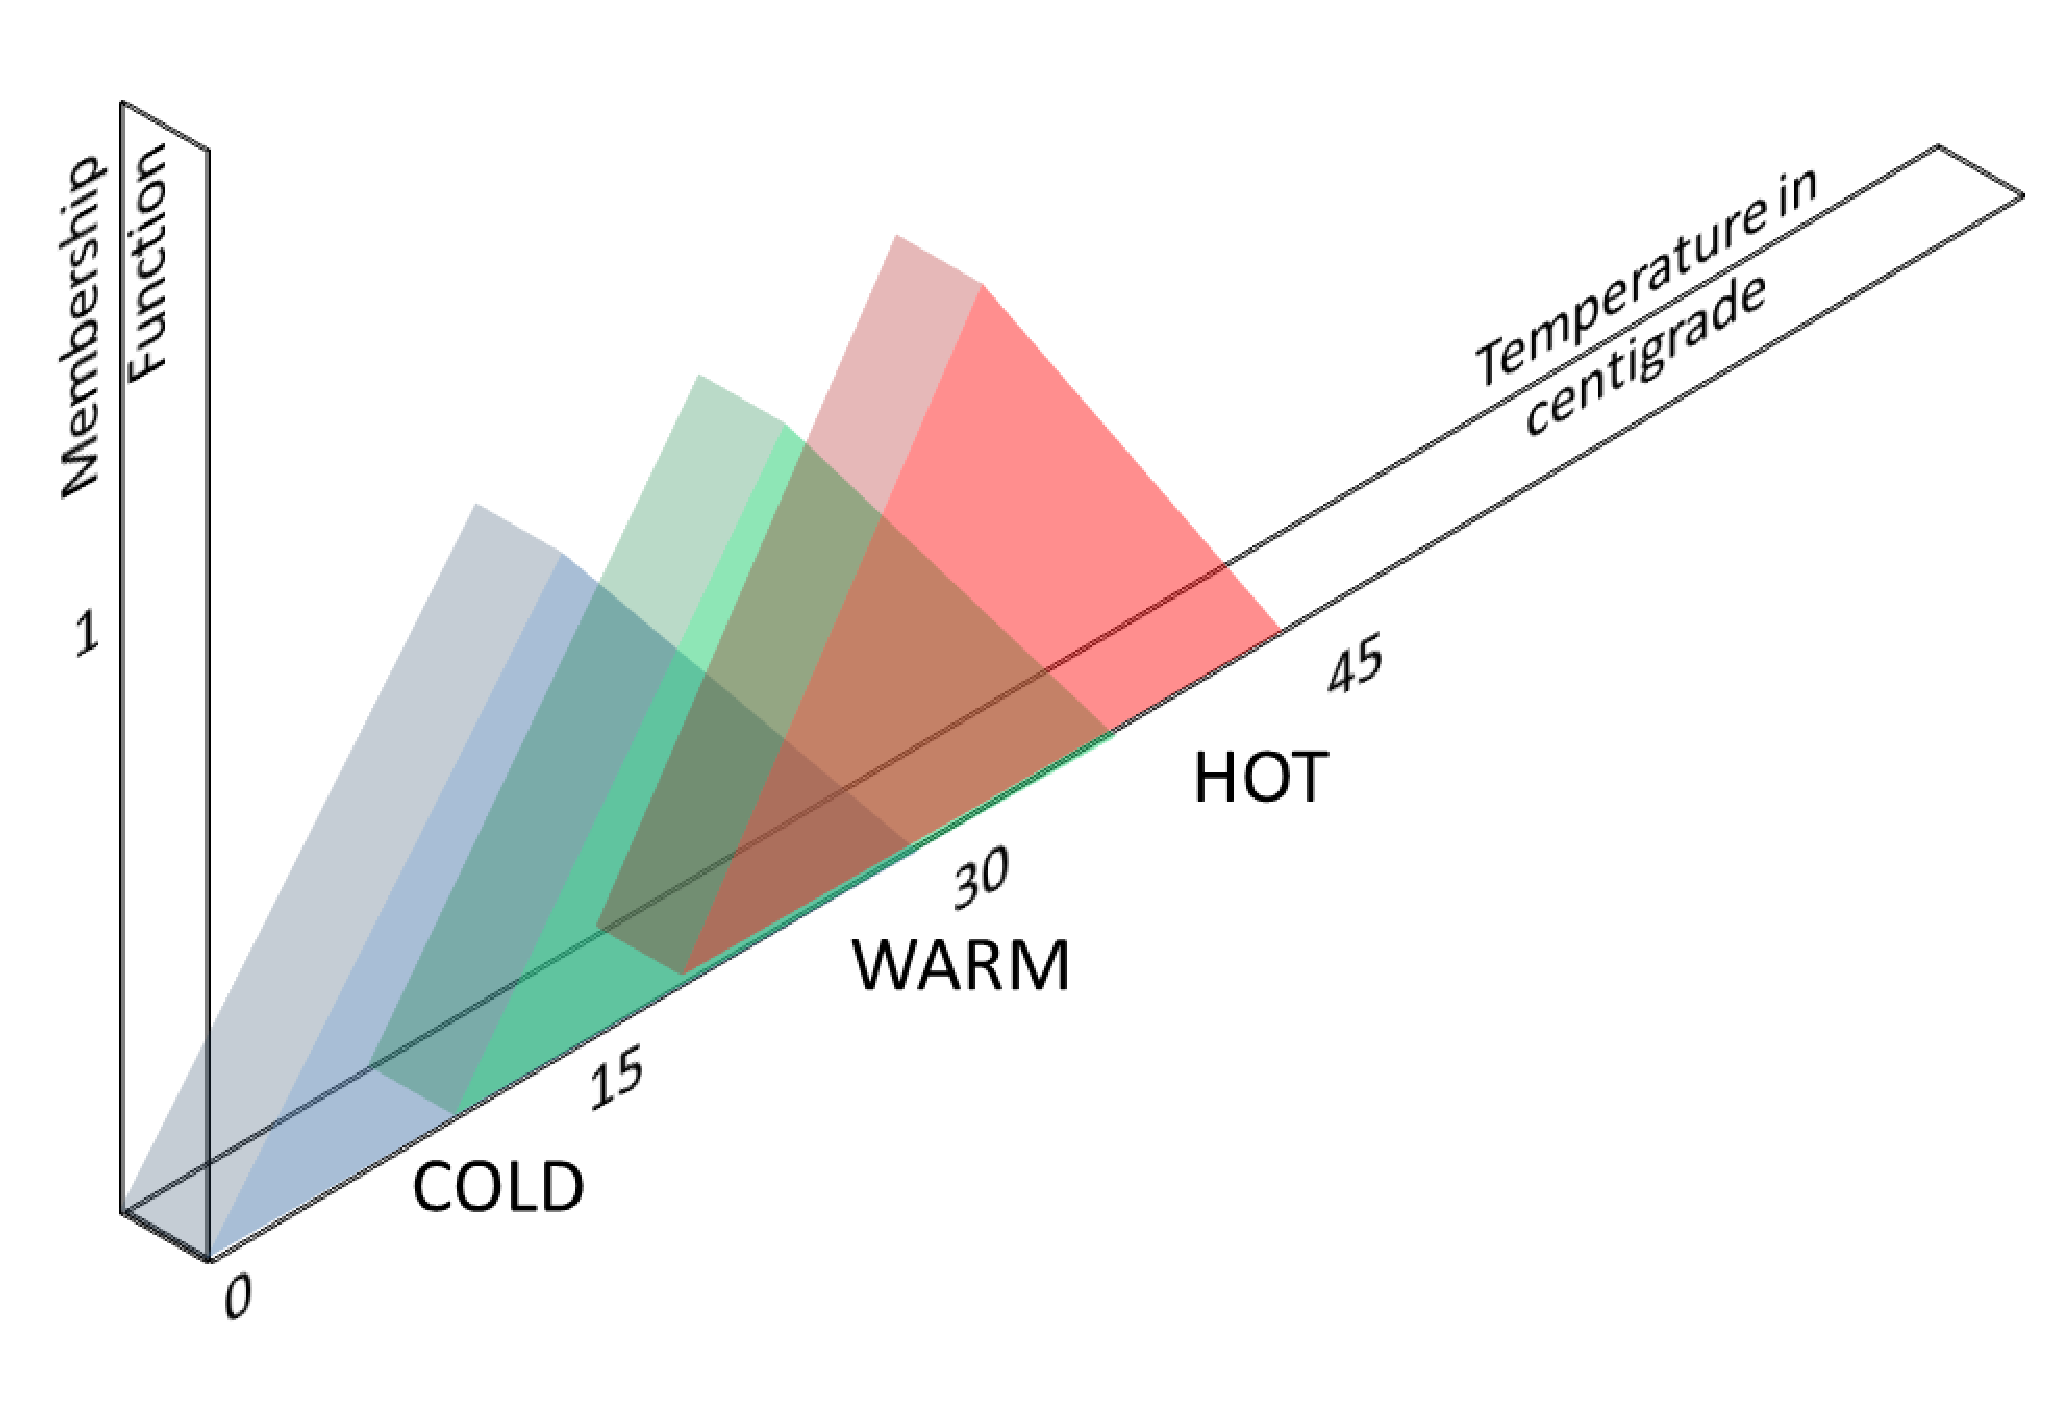
\includegraphics[width=0.8\linewidth]{Chapter1/chapter1/Fig5_f_set}
\caption{Fuzzy sets to model room temperature}
\label{fig:Fig5_f_set}
\end{figure}

Mathematically, a fuzzy set is a pair $ \left( {\xi ,\mu } \right) $, where $ \xi $ is a set, also known as universe of discourse, and $ \mu :\xi  \to \left[ {0,1} \right] $. This implies that $\mu$ presents the degree of association of an element to the set $\xi$ which lies in between $\left[ 0,1\right]  $. Therefore, $ \forall x \in \xi ,\mu \left( x \right) \to [0,1] $, where $ \mu \left( x \right) $ is called the grade of membership for $ x $, $ x $ being a fuzzy number in fuzzy set $\xi$.

A set $\left\{ {x \in \xi |\mu \left( x \right) > 0} \right\}$ is called support and set $\left\{ {x \in \xi |\mu \left( x \right) = 1} \right\}$ is called core or kernel \cite{bookBogdan2006a,Ross2010}. The function $ \mu $ is called membership function (MF) of fuzzy set $ \left( {\xi ,\mu } \right) $\cite{bookBogdan2006a,Ross2010}.

A fuzzy system operates on various fuzzy sets to provide a suitable output. It is often required that these fuzzy sets are combined meaningfully. Various combination operators exist in ordinary set theory, and it is imperative that there exist a commonality of operators between regular and fuzzy sets. These operators are termed as \textit{aggregators} \cite{Nguyen2003}.

\section{Fuzzy Operators}
Ordinary sets are combined or negated by using operators like intersection (AND), union (OR), and complement (NOT) \cite{Nguyen2003}. Similarly in fuzzy sets, minimum, maximum and negation operators approximate AND, OR and NOT operations. However, on many occasion, \textbf{AND} operations can be achieved by functions other than the minimum operation. These functions are collectively referred to as triangular norms or simply as t\hyp{}norms. Similarly, \textbf{OR} operations are referred to as triangular co\hyp{}norms or t\hyp{}conorms or s\hyp{}norms\cite{Ross2010,bookBogdan2006a}.
%bookponce2010,

There are four basic t\hyp{}norms and almost all t\hyp{}norms used in a fuzzy system are derived from these basic operations \cite{bookBogdan2006a}. Consider $\mu _x$ and $\mu _y$ as membership grade of two fuzzy numbers $ x $ and $ y $, in a fuzzy set. Then the following equations represents the various t\hyp{}norm operations in a fuzzy system.
\[\begin{array}{l}
1. \text{Zadeh Intersection:} ~~~T\left( {{\mu _x},{\mu _y}} \right) = \min \left( {{\mu _x},{\mu _y}} \right)\\
2. \text{Product Intersection:} ~~~T\left( {{\mu _x},{\mu _y}} \right) = \left( {{\mu _x} \cdot {\mu _y}} \right)\\
3. \text{Lukasiewicz Intersection:} ~~~T\left( {{\mu _x},{\mu _y}} \right) = \max \left( {0,\left\{ {{\mu _x} + {\mu _y} - 1} \right\}} \right)\\
4. \text{Basic Intersection:} ~~~T\left( {{\mu _x},{\mu _y}} \right) = \left\{ {\begin{array}{*{20}{c}}
	{{\mu _x},~~~if{\mu _y} = 1}\\
	{{\mu _y},~~~if{\mu _x} = 1}\\
	{0,~~~if{\mu _x},{\mu _y} < 1}
	\end{array}} \right.
\end{array}\]

Similarly, the t\hyp{}conorm or s\hyp{}norm operators can be represented as following equations in a fuzzy system \cite{bookBogdan2006a}.
\[\begin{array}{l}
1. \text{Zadeh Union:} ~~~S\left( {{\mu _x},{\mu _y}} \right) = \max \left( {{\mu _x},{\mu _y}} \right)\\
2. \text{Product Union:} ~~~S\left( {{\mu _x},{\mu _y}} \right) = {\mu _x} + {\mu _y} - \left( {{\mu _x} \cdot {\mu _y}} \right)\\
3. \text{Lukasiewicz Union:} ~~~S\left( {{\mu _x},{\mu _y}} \right) = \min \left( {0,\left\{ {{\mu _x} + {\mu _y} - 1} \right\}} \right)
\end{array}\]

There three major fuzzy complement operators which have been widely used in the literature \cite{bookBogdan2006a}. These operators are;
\[\begin{array}{l}
1. \text{Standard Complement:} ~~~N\left( \mu _x \right) = \left( 1 - \mu _x\right)\\
2. \text{Sugeno's Complement:} ~~~{N_s}\left( {{\mu _x}} \right) = \frac{{1 - {\mu _x}}}{{1 + s{\mu _x}}}\\
3. \text{Yager's Complement:} ~~~N\left( \mu _x \right) = \left( {{\mu _x} \cdot {\mu _y}} \right)
\end{array}\] 
where $ s $ is Sugeno's constant and $ w $ is Yager's constant.

\section{Fuzzy Rules}
Words rather than numbers define linguistic variables. Fuzzy rules use these linguistic variables instead of numbers to quantify variables.  These linguistic variables are represented as fuzzy sets with a certain function. This provides the mathematical background of the fuzzy systems. All fuzzy rules are divided into an antecedent part (starting with ``$IF \ldots $'')
and a consequent part (ending with ``$THEN \ldots $''). The antecedent parts describe the causes while the consequent parts describe effects relevant to desired control action. A typical form of a fuzzy rule with Rulebase index $ {R_b}\left( k \right) $ is as shown below.
\[{R_b}\left( k \right):~~~~\text{If}~i_1\text{ is }{a_1}~\text{and}~i_2\text{ is }{a_2}~\text{and}~\cdots \text{and}~i_N\text{ is }{a_N},~\text{then output is }~{c_j}\]
where, $ {i_1},{i_2} \cdots {i_N} $ represents inputs,  $ {a_1},{a_2} \cdots {a_N} $ are called antecedent and $ c_j $ is the resultant consequent.
All antecedents and consequents are represented by valid linguistic variables in a fuzzy system.
\section{Fuzzy Logic Control System}
Traditionally, the industrial process control was dominated by binary logic based reasoning. Heuristic knowledge hardly plays any role in these systems \cite{bookBehera2009,bookMichels2006}. This forced the systems to be represented by a collection of complex mathematical equations. The drive for precise and accurate control was expensive and often proved to respond sluggishly. However, in recent past, the power of human reasoning started to get acknowledged with the advent of FLCS in nonlinear process control \cite{Zadeh1993,Mendel1995,Sugeno1985,Mendel2000}. The most appreciable feature of FLCS is its ability to manage complex control problems through human knowledge and numerical models provided by fuzzy set theory, instead of using complex differential equations to derive mathematical models of  a process plant.

The computing framework of a fuzzy logic control system (FLCS) rely on three conceptual components:
\begin{description}
	\item[i. Rulebase:] This contains a database of rules that represent human knowledge and heuristics. They define I/O relationship of the system in terms of linguistic variables.
	\item[ii. Database:] This defines the MFs that are used to define the linguistic variables in the fuzzy rules. 
	\item[iii. Inference Mechanism:] This performs the reasoning procedure based on the Rulebase and Database.
\end{description}
These three components together constitute the Fuzzy Control Parameters (FCP). At this juncture, an operator's experience and knowledge is appropriately formulated and configured into FCP. This FCP represents the ``intelligence'' in any fuzzy control algorithm. Hence, it can be asserted that the information of the FLCS is dependent on the knowledge of the designer or the operator.

\begin{figure}[t!]
	\centering
	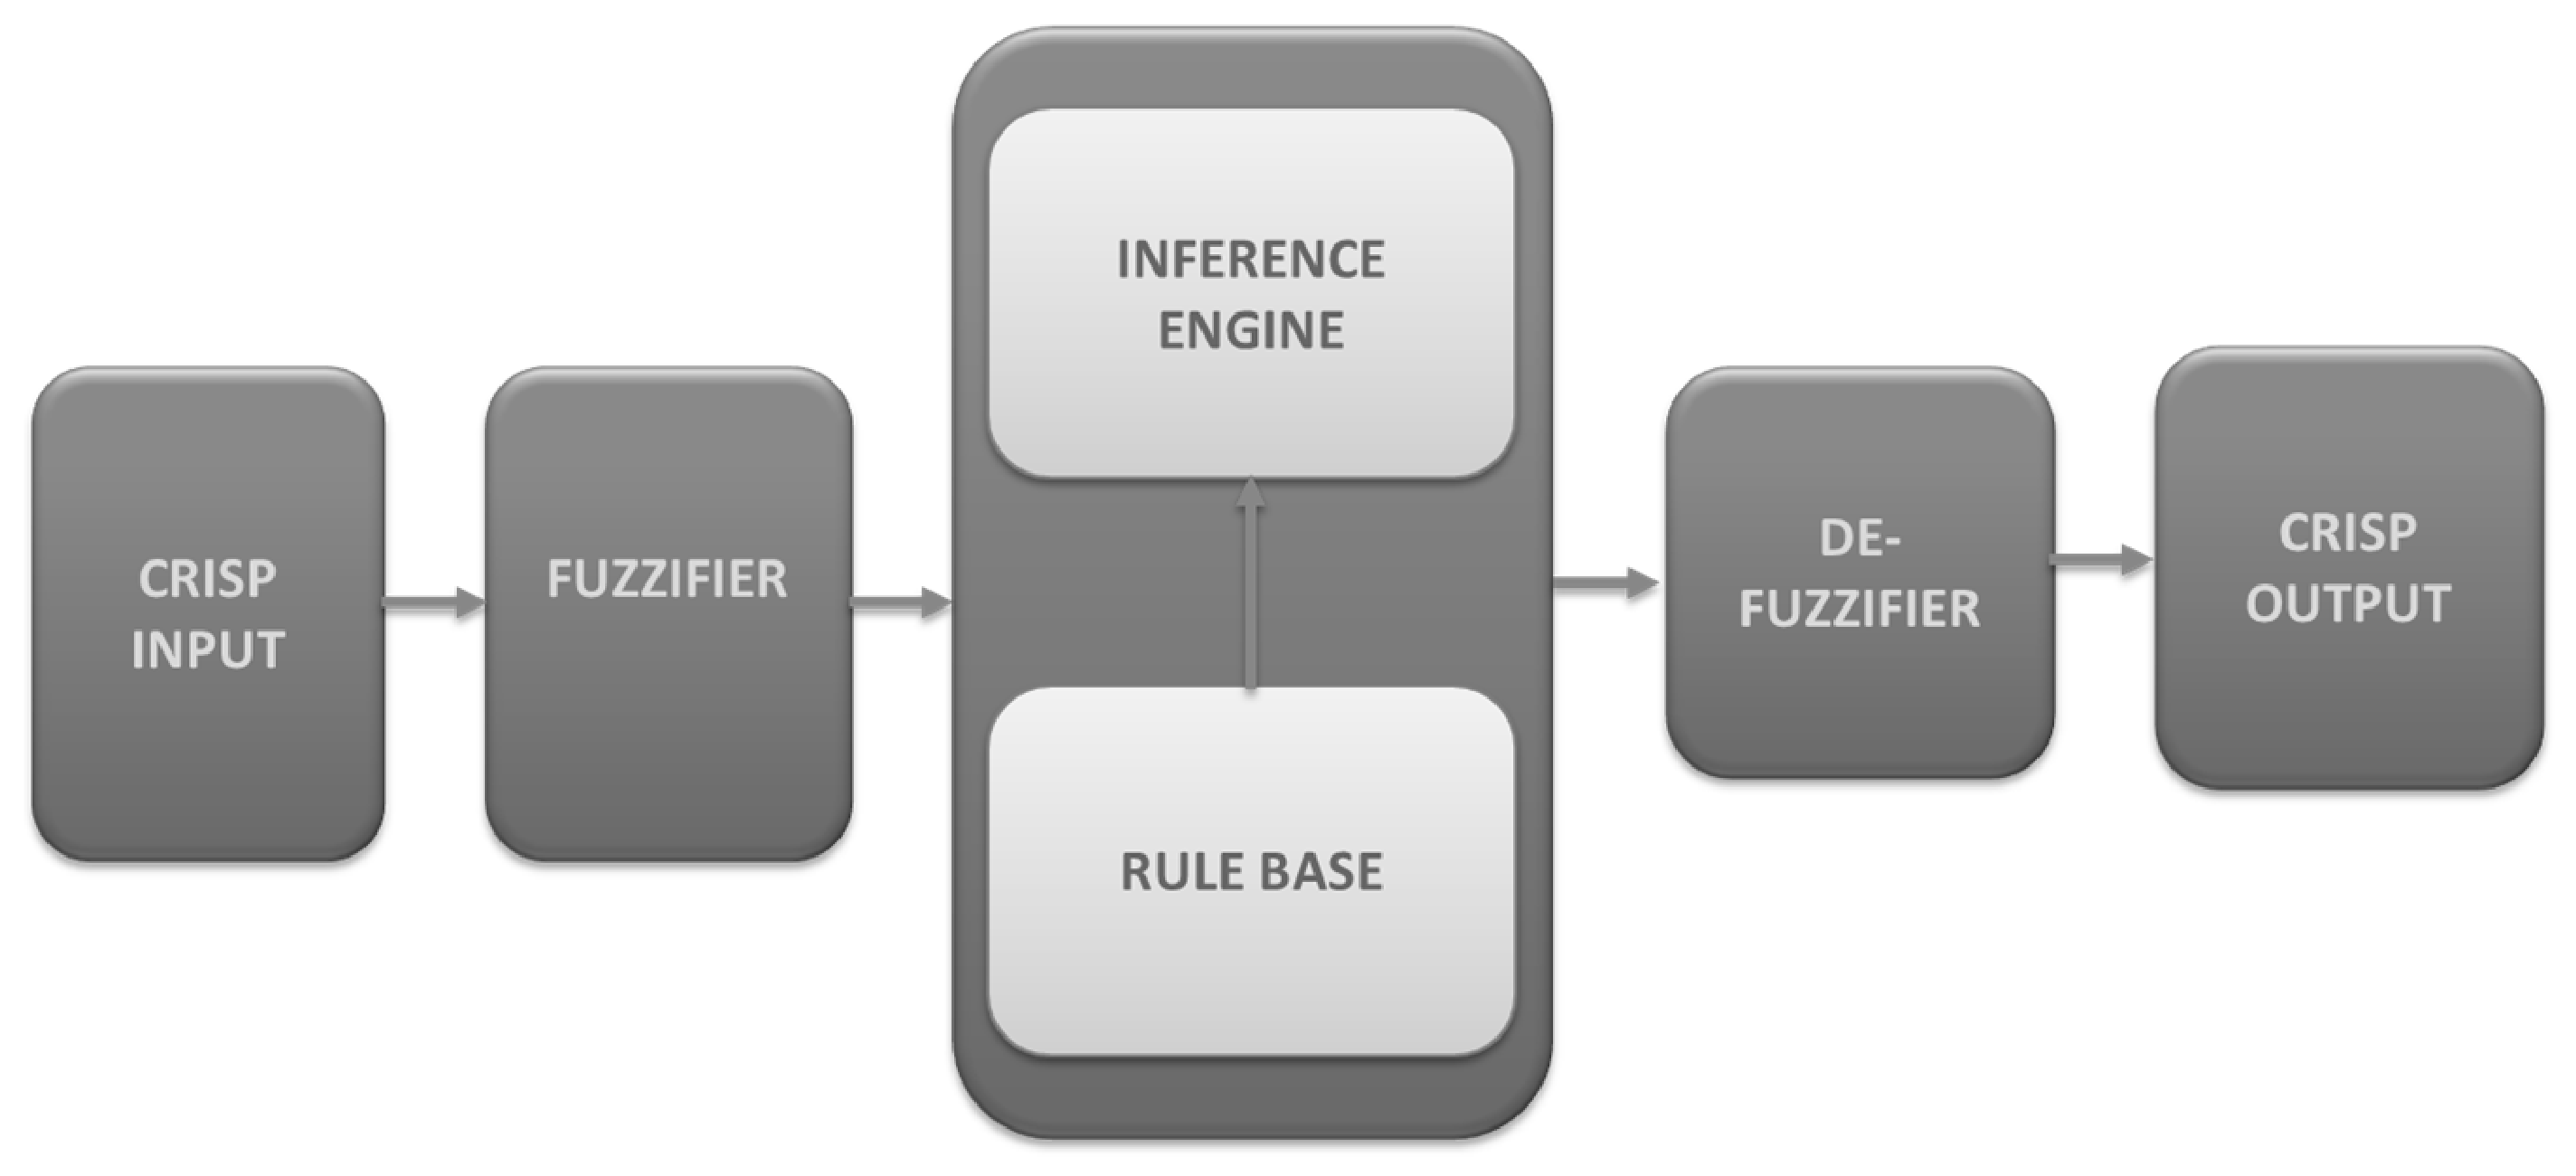
\includegraphics[width=0.9\linewidth]{Chapter1/chapter1/Fig1_FLCS}
	\caption{Black diagram of a FLCS}
	\label{fig:Fig1_1}
\end{figure}

FLCS has four important modules which interact with the input to generate a meaningful output\cite{Wang1997,bookMichels2006,Mendel1995}. The block diagram of the modules in a FLC is represented in Figure \ref{fig:Fig1_1}. These modules are;
\begin{description}
	\item[i. Fuzzifier:] The input variables in a fuzzy control system that are real world variables and also known as \textit{crisp input data}, are in general mapped by sets of membership functions, known as ``fuzzy sets''. The fuzzifier generates a set of output in between 0 to 1, which are dimensionless. This process of converting a crisp input value to a set of fuzzy values is called ``fuzzification''.
	\item[ii. Rulebase:] It stores the heuristic rules that govern a typical fuzzy system. These rules describe the output dependence of the inputs, and they are  mentioned in terms of the MFs representing the inputs and outputs of the process plant.
	\item[iii. Inference Engine] It accepts fuzzified inputs and applies reasoning described by the Rulebase to work out fuzzy outputs.
	\item[iv. Defuzzifier:] It translates fuzzy outputs from the Inference Engine into substantive crisp output applicable to a real system.
\end{description}


\section{Learning of FCP from Data} \label{sec:learnFCP}

Learning of FCP from data essentially means designing or extracting parameters that governs the fuzzy controllers from a given sampled data or model of a system. According to Wang et. al. \cite{Wang1992a} there are five steps in this process. 
\begin{description}
	\item[Step 1] The input and output spaces are recognized and divided into fuzzy regions.
	\item[Step 2] The dataset is observed and fuzzy rules are generated from it.
	\item[Step 3] Each generated rule is assigned a degree to resolve any conflict that arises amongst the generated rules.
	\item[Step 4] Based on visualization paradigm and human expert knowledge, some rules can be directly inferred about the system. These rules are combined with the generated rules.
	\item[Step 5] Once the rulebase is formed, the ouput in fuzzy domain can be obtained. This output is mapped to real world output using a suitable defuzzification procedure. 
\end{description}

In the context of learning FCP, Step 1 to 3 can be manual or it can be formulated as a learning problem itself. G. D. Finn proposed `Fuzzex' for generating fuzzy rules in general from data \cite{finn1999learning}. In this popular technique, they proposed a five step method where cell occupancy is used. But this method does not suit nonlinear system approximation. In 2009, Sánchez et. al., presented a genetic algorithm based learning method which is robust to system noise \cite{sanchez2009genetic}. Tuning fuzzy rules using genetic algorithm has been widely investigated and is often the most popular choice \cite{Surmann2001,Sanz2011,Uddin2007a}. However, learning the entire FCP is a difficult task at hand. To counter this issue, a new strategy for sophisticated learning of FCP with Genetic Algorithm optimization technique is proposed in Section \ref{sec:FCP}. 

\section{Motivation of This work}
PID controllers are widely used in industries even though they are inherently linear and provides a sluggish response. They are generally not suited to control nonlinear process plants \cite{Atherton1999a,Bennett1996,Atherton1999}. Their modeling requires a thorough knowledge of system dynamics and the tuning process is quite difficult too. Fuzzy Logic Controllers (FLC) provide an imprecision based control approach which is fast and reliable. However, they are driven by the human knowledge which is prone to be erroneous. Some designs provide techniques to derive the FCP from a dataset or model. However, this eradicates human knowledge completely. Therefore, it is highly desirable to have a FLCS with two level tuning.
\begin{itemize}
	\item Coarse Tuning: Achieved by using suitable algorithm and FCP are extracted,
	\item Fine Tuning: Using an interface, system is fine tuned by an operator.
\end{itemize} 

\section{Objective of this work} \label{sec:obj}
Fuzzy logic systems have found applications in a variety of fields namely industrial process control, power systems, robotics, water resources, structural design, metallurgy and material science, business and finance, and many more. It is challenging for scientists and engineers to implement an efficient FLCS design that can be integrated into their system of interest, especially if they are not well equipped with knowledge of programming and system development. Therefore, the primary objective of this research is to design and realize a generic fuzzy logic controller system (G\hyp{}FLCS) on a programmable hardware that can be used for a variety of applications without reprogramming. Some of the characteristic features of this proposed control device will include
\begin{itemize}
	\item Plug and play framework: Essentially process plant operators are not good programmers. It is, therefore, mandatory for a controller device to possess a plug and play framework for ease of installation and operation. Users can input the fuzzy parameters through an interactive user interface.
	\item Runtime tunability: Most control device lacks this feature. The major advantage of run\hyp{}time tunability is that it provides an opportunity to include the concept of two level tuning, one of the prime motivating factor for this research. This will offer the leverage to fine-tune the FLCS while it is in operation so that the parameters can be reset to default under critical conditions.
	\item Standalone operation: The prime requirement of any real\hyp{}time system or controller is to be able to operate in a standalone mode.
	\item Flexibility in operation order: A G\hyp{}FLCS system primarily implies that it can be implemented on any system with appropriate parameter tuning; be it a single\hyp{}input\hyp{}single\hyp{}output system or multiple\hyp{}input\hyp{}multiple\hyp{}output system. Thereby, it is implicit that the G\hyp{}FLCS should have the provision to accommodate a different number of inputs and outputs.
\end{itemize}
It becomes a challenging task when run\hyp{}time tunability, flexibility in system order and plug and play framework is combined with the standalone mode of operation. Therefore, the architecture of traditional FLCS is required to be altered in a way such that, the data integrity and operational methodology remains consistent even after incorporating the above-mentioned features.

\section{Literature Survey on Design and Implementations for FLCS on various Hardware Platforms}
%FLC application, need for hardware implementation.
In recent times fuzzy logic is addressing complex problems of control, forecasting and prediction with imprecision in fields of robotics \cite{Linda2011,Acevedo2013,Das2006,Lochan2015,Das2006,Gopinath2008}, chemical \cite{Foerster2013,Pan2005,Aqlan2014,Khoshnevisan2014,Lerkkasemsan2014,Shamiri2015} and manufacturing processes \cite{Zammar2015,Rajak2015,Gokulachandran2015}, automobiles \cite{Wang2015,Baldania2014,Basjaruddin2015,Li2014b,Bogdan2008}, business and finance\cite{Korol2014,Tung2004,Yoshida2003,Dostal2013}, power electronics \cite{Bhende2006,Lou2015,AlNabulsi2012}, and many others\cite{Dostal2013,Kumar2015,Kumar2015a,Sun2015,Boumaaraf2015,Jadoun2015} in a better way than conventional control techniques. Wide spread application of the FLCS and its extensively high effectiveness to a larger extend
is driven by formalizing necessary human knowledge and sometimes behavior in the controller as an imprecise and approximate representation. These factors impel engineers to design and implement fuzzy based controllers for wide array of applications.

The hardware designs of FLCS can be classified into three broad categories based on their circuit architecture.
\begin{itemize}
	\item Analog, 
	\item Digital, and  
	\item Mixed Signal
\end{itemize}
Each of these can be further classified based on the aspect of system design and platform for implementation. 
\begin{description}
	\item[Dedicated Integrated Circuits:] These FLCS are designed primarily to target a single control application. These devices are mostly built over application specific integrated circuits (ASIC) and implement full custom analog, digital or mixed-signal designs \cite{Idros2014,Matsumoto2014,Li1997,Gomariz1998,Malek2008,Costa1995}.
	\item[Programmable Integrated Circuits:] Programmable Integrated Circuit based FLCS devices are commercially developed in integrated circuits (ICs) that can be reconfigured by the user. These tools provide attractive options to designers and engineers. They have the ability to be reprogrammed, and their high integration density is a fascinating feature. Commercially available field programmable gate arrays (FPGAs) and field programmable analog arrays (FPAAs\footnote{This is an integrated device comprising of configurable analog blocks (CAB) and in between interconnects. Lattice and Anadigm are prime manufacturers of this device.}) have been widely used in designing of these systems \cite{Guajardo2007,Sun2015a,Monmasson2007,Cecati2010,Palakeerthi2014,Jabeen2008,Tran2015,Pierzchala1998}.
	\item[Commercial Processors:] A software application defining the system is developed and deployed on these devices. Microprocessors ($\mu$P), Microcontrollers ($\mu$C) and Digital Signal Processors (DSPs) based systems are defined under this category \cite{Santoso2014,Youness2014a,Kurniawan2015,Yousef2015,Jia2011,Oswald2014,Selvaperumal2014}.
\end{description}

\begin{table}[t!]
	\centering
	\caption{Taxonomy for Hardware Implementation of FLCS}
	\label{tab:tax}
	\begin{tabular}{clll}
		\hline
		\multicolumn{1}{l}{} & Classification & Platform & Devices \\ \hline
		\multicolumn{1}{c|}{\multirow{9}{*}{\begin{tabular}[c]{@{}c@{}}Types of\\ Implementation\end{tabular}}} & \multicolumn{1}{l|}{\multirow{3}{*}{Analog}} & Dedicated IC & Analog ASIC \\
		\multicolumn{1}{c|}{} & \multicolumn{1}{l|}{} & Programmable IC & FPAA \\
		\multicolumn{1}{c|}{} & \multicolumn{1}{l|}{} & Commercial Processor & -- \\ \cline{2-4} 
		\multicolumn{1}{c|}{} & \multicolumn{1}{l|}{\multirow{3}{*}{Digital}} & Dedicated IC & Digital ASIC \\
		\multicolumn{1}{c|}{} & \multicolumn{1}{l|}{} & Programmable IC & FPGA, CPLD \\
		\multicolumn{1}{c|}{} & \multicolumn{1}{l|}{} & Commercial Processor &  \\ \cline{2-4} 
		\multicolumn{1}{c|}{} & \multicolumn{1}{l|}{\multirow{3}{*}{Mixed}} & Dedicated IC & Mixed Signal ASIC \\
		\multicolumn{1}{c|}{} & \multicolumn{1}{l|}{} & Programmable IC & -- \\
		\multicolumn{1}{c|}{} & \multicolumn{1}{l|}{} & Commercial Processor & -- \\ \hline
	\end{tabular}
\end{table}

Different forms of FLCS implementation is presented in Table \ref{tab:tax}. The forms of FLCS include;
\subsection{Analog Implementation of FLCS Design}
A Large number of FLCS in literature have been developed on analog devices. The major reasons that drive a FLCS design engineer to choose these platforms are high parallelism, high speed, low area and low power consumption \cite{Soleimani2010,Soleimani2014,Baturone1996,Peyravi2002}. Different forms of Analog IC based implementation includes;
\subsubsection{Dedicated IC based FLCS}
There are three modes in which these devices are implemented namely,
\begin{description}
	\item[Current Mode] implementation uses fewer transistor and hence they consume low power. However, these devices can only connect to one output since they work in current mirror mode \cite{Bosque2014b,Zavala2012}. Some of the work those were developed using these techniques are
	\begin{itemize}
		\item Tokmakci et. al.\cite{TokmakcI2008} designed current\hyp{}mode CMOS FLC. The membership function circuit (MFC) implemented trapezoidal, triangle, Z\hyp{}shape and S\hyp{}shape MFs. which were tunable by two voltages through switches.{ The system developed was a two\hyp{}inputs\hyp{}one\hyp{}output with 9 tunable rules only}. The operation speed of this FLCS was reported to be 6.25 Mega Fuzzy Logic Inferences per second (MFLIPS)\cite{TokmakcI2008}.
		\item Gheysari et. al.\cite{Gheysari2011} proposed a Flexible Structured Fuzzy Logic Controller Chip (FS\hyp{}FLC) on $ 0.35 \mu m $ process. They implemented Ordered Weighted Averaging operator to aggregate multiple\hyp{}input single\hyp{}output (MISO) system.{ However, the FLCS design used singleton rules at output. }
	\end{itemize} 
	\item[Voltage Mode] implementation of FLCS can serve more than one outputs unlike current-mode. Some of the noted designs include
	\begin{itemize}
		\item Mokarram et. al.\cite{Mokarram2015}: developed a two\hyp{}input, single\hyp{}output Takagi\hyp{}Sugeno\hyp{}Kang (TSK) FLC on $ 0.35 \mu m $ standard CMOS process. The system supports triangular and trapezoidal membership functions. Membership function generator (MFG) provides generation and tuning of the MFs but {the design do not permit changing or tuning of rules}.
		\item Aminifar et. al.\cite{Aminifar2012}: The designed a FLCS on $ 0.35 \mu m $ CMOS process with inference speed of 14.83 MFLIPS. {They designed a 2\hyp{}input one\hyp{}output system with mere 9 rules with support to only singleton MFs at output. Moreover, the design do not allow any tunability.}
	\end{itemize} 
\end{description} 

\subsubsection{Programmable IC based FLCS}
There has been very limited research reported on FLCS implementationAnalog Programmable ICs. Some of the most significant works include;
\begin{itemize}
	\item Amaral et. al\cite{Amaral2004} designs and developed in PAMA\hyp{}NG, a FPAA platform, with I/O board connected to the PCI bus of the PC. The system used Genetic Algorithm (GA) to reconfigure the FPAAs. 
	\item Ionita et al.\cite{Ionita2005} also used evolutionary algorithm to tune MFs. They developed a Mamdani type FLCS on FPAAs.
\end{itemize}
{It has been observed that designs implemented on Analog Programmable ICs are extremely sensitive to problems of fanout and presence of switches on the signal path \cite{pierzchala2013field}. It is also known that analog circuits are more vulnerable to be affected by noise in comparison to Digital circuits.}

\subsection{Digital Implementation of FLCS Design} 
Fuzzy systems and control are making fast advancement in past decade and two. Owing to its pragmatic achievements in consumer electronics and industrial process control, implementation of FLCS has been rigorously researched and developed. However, increase in process complexity of the industrial plants is accelerating demand for controllers with high computational speed, low complexity, easy deployment, comfortable handling and less development time in terms of design. {In order to conform to the demand\hyp{}supply chain of the industry, FLCS have to be designed accordingly.} A noteworthy solution to fulfill this growing market demand is to move to a digital platform. It is well known that digital systems have high resistance to noise, temperature and voltage variations. There is a vast array of digital platforms available to an engineer for design implementation that reduce turnaround time. Although, systems designed in digital hardware platforms are not as fast as analog designs; still a good system cycle time can be achieved which provide sufficient throughput speed for the majority of the control problems. Table \ref{tab:tax} shows the various digital implementation platforms for realization of different FLCS designs.

\subsubsection{Dedicated IC based FLCS}
These implementations concentrate on structuring the fuzzy rules in a FLCS and its functionality is defined by, whether these rules are evaluate sequentially or in parallel. Some of the notable designs include
\begin{itemize}
	\item Eichfeld et. al.\cite{Eichfeld1992} reported a four\hyp{}input single\hyp{}output FLCS with 4096 rules with eight MFs for each input. However, the system {operated only on two overlapping MFs and used singleton type MFs for output}.
	\item Jacomet et. al.\cite{Jacomet1996} described an architecture of a VLSI fuzzy processor fabricated in the $ 0.7 \mu m $ digital CMOS process. High performance was achieved due to its parallel architecture. The FLCS evaluates 64 rules but {this design too uses two overlapping MFs scheme. Moreover, if four inputs are used, the rules are limited to 64 and thereby, only 3 MFs per input were allowed}.
	\item Huang et. al.\cite{Huang2005} developed a FLCS in $ 0.35 \mu m $ CMOS process. {However, this design used trapezoidal MFs only with a fixed rulebase.}
	\item Hamzeh et. al.\cite{Hamzeh2009} designed one of the most flexible structure for FLCS in the literature. {This device however do not discuss the speed of performance.}
	\item Javadi et. al.\cite{HajiSeyedJavadi2012}'s design provides a new fuzzification method for hardware on $ 0.13 \mu m $ but it is {only applicable to piece\hyp{}wise linear MFs.}
\end{itemize}

\subsubsection{Programmable IC based FLCS}
\paragraph{CPLD based FLCS Design}
It has been shown in Table \ref{tab:tax} that there are two preferred devices which can be categorized in this segment, namely FPGA and complex programmable logic device (CPLD). There are very few CPLD based designs reported in literature. Some of the important designs are,
\begin{itemize}
	\item Hongguo Sun et. al. \cite{Sun2013} presented a Fuzzy PID design on CPLD for PWM trigger pulse generation to a full bridge inverter and a chopper circuit. {It implemented a two\hyp{}input one\hyp{}output FLCS with fixed rulebase and rigid MFs}.
	\item Jingyan Xue et. al. \cite{Xue2009} presented a novel methodology to design a fuzzy reasoning based expert system on CPLD for fault diagnosis. Similar to previous design,{ this too implemented a FLCS with fixed rulebase and rigid MFs.} 
\end{itemize}
There are not many CPLD based FLCS designs that are reported in literature. The decisive reasons are that CPLDs are cost and power intensive platform. Moreover, there are platforms which are easy to configure than CPLDs.

%INCLUDE FPGA based LIT SURVEY
\paragraph{FPGA based FLCS Design}

\begin{itemize}
	\item Adhavan et. al. \cite{Adhavan2014a} countered the problem of non-uniform variance of the torque developed in a vector controlled permanent magnet synchronous motor by introducing a FIS implemented on an FPGA. Author have reported that the heuristic knowledge based FLCS (Fuzzy Logic Control System) has reduced the torque ripple to 1.81\%.
	\item Ben, Zekeri et al. \cite{Benzekri20146109} reported PD approximated FLCS developed on cyclone II FPGA to control a dual axis sum tracking systems.  The simple rules developed with human knowledge have been found to be successful in reducing chip count, cost and development time of the controller significantly.
	\item Santo and Ferreira \cite{Santos2014} implemented a multi-state FLCS on virtex II FPGA and NI compact $ R10-9002 $ to control servo- pneumatic actuation systems.  They showed significant performance gain in term of steady state error, overshoot and settling time.
	\item Messai et. al. \cite{Messai2011} reported a FLC to seek maximum power point deliverable by a photovoltaic (pr) module using measures of PV voltage and current.
	\item Schriber et. al. \cite{Schrieber2015}presented an interval type- II FLCS implemented on a xiling spartan 6 FPGA utilizing DSP48AI slices for different linear and non-linear modules.
	\item Tamukoh et. al. \cite{Tamukoh2007} reported a new technique of bit shift based fuzzy inference method for an efficient digital hardware implemented. They implemented the proposed design on a virtex II FPGA for a self-organization relationship network. 
\end{itemize}
	These designs depicts that the realization of FLCS on FPGA development platform is fast and efficient. However most of these designs are application specific. It is important to realize that even  the speed achieved by these designs cannot to achieved by any generic FLCS design as these appears a large amount of branching in the G-FLCS algorithm.	
\paragraph{Digital ASIC Design based FLCS Design}	
	\begin{itemize}
		\item Martinez-rodriguez \cite{Martinez-Rodriguez2015} has presented a FLCS on ASIC platform where the number of input to and output MFs can be varied on run time. {However, in this design, the number of configurable parameters are very few with a rigid rulebase.}
		\item Evmorfopoulos et. al. \cite{Evmorfopoulos2002} reported a G\hyp{}FLCS structure on digital ASIC which can {had a maximum of five MFs at the input. All input MFs were Gaussian type and output MFS are singleton type.}
		\item D'Amore \cite{DAmore2001} reported a bit scalable fuzzy processors with three input and MF generators. {However like the previous design, this system do not equate with output MFs other than singleton type too. }
	\end{itemize}
	Digital ASIC design is generally quite time intensive in development and the process incurs extreme cost. Without large production, these designs are not cost-effective solution.
%INCLUDE DSP based LIT SURVEY
\subsubsection{Commercial Processors based FLCS}

\paragraph{FLCS Implementation with TMS320F Series DSP}
\begin{itemize}
	\item EL Khatib et. al. \cite{ElKhateb2014} presented a FLCS based SEPIC converter on TMS32F28335 DSP device to successfully track the reference signal using MPPT to transfer power around 4.8\% than conventional PI based system.
	\item Eskandarin et.al \cite{Eskandarian2014} proposed a fuzzy instantaneous power theory to improve conventional p-q theory dynamic performance and implemented it on a TMS320F28335 DSP device.
	\item Okumus et. al. \cite{Okumus2014} has reported on FLCS design implementation of TMS320F2812 DSP device to control a brushless DC motor and compared the result with HB current controller. The heuristic knowledge based FLCS is found to perform extensively well.  
\end{itemize}

\paragraph{FLCS Implementation with TMS320C Series DSP}
\begin{itemize}
	\item Uddin et. al. \cite{Uddin2007} showed a cost effective FLCS based controller designs on TMS320C31 DSP to control an interior permanent magnet synchronous motor for high performance industrial applications.
	\item S. Gai et al. \cite{Gai2010} used a TMS320C6713 DSP device to implement a fuzzy based Haar wavelet feature extraction technique to successfully classify and detect a counterfeit banknote.
\end{itemize}

\paragraph{FLCS Implementation with dSpace DSP}
\begin{itemize}
	\item Butt et. al. \cite{Butt2004} implemented FLCS based MTPA speed control of a IPMSM drive on a DS1102 DSP.
	\item Like many FLCS designs reported on tracking of maximum power point using MPPT algorithm Noman et. al. \cite{Noman2013} also proposed a FLCS design for similar application using a DS1104 DSP.
	\item Rafa et. al. \cite{Rafa2014} implemented a new FLCS design on DS1104 DSP to solve coupling problem in vector control of induction motor.
	\item Rubaai et. al. \cite{Rubaai2007} used DS1104 to implement a FLCS control structure with adaptive la based Lyapunov synthesis for trajectory tracking control of a brushless servo drive systems.
\end{itemize}

There are many more DSP based FLCS designs that have been successfully implemented in various control applications. It can be readily inferred that the development of DSP based FLCS is easy compared to FPGA \cite{Parker2010,Lall2002Xilinx,Schneiderman2014}. However, since the parallel architecture can be implemented on FPGA, DSP likes sequential processors are preferred less while developing application specific FLCS \cite{altera2007}. Moreover, the number of branching infractions are extensively reduced in application specific FLCS design as the fuzzy parameters are fixed. This makes FPGA platform more preferable. However for GFLCS design, the situation is quite inverse. In next section, it will be explained why DSP is preferred over FPGA for this particular research work.

\section{Inference from the Literature Survey}
The previous section have laid down the various FLCS designs and some essential features in their implementation. It would be beneficial to summarize the prime aspects of these designs. In this section, a brief inference of the literature survey is portrayed.
\subsection{FLCS Implementation in FPGA and DSP Platforms}
FPGAs and DSPs are most widely used programmable devices for digital implementations of various algorithms \cite{Jinghong2007,Buccella2012,Bilsby1998}. Traditionally, manufacturers like Texas Instruments(TI) and Analog Devices developed processors for specifically for signal processing applications and called them DSP. These are most still most preferred platform for signal processing applications \cite{Lall2002Xilinx}. However, the unsatisfiable need for gadgets that require higher performance and address complex algorithms is driving growth that is hard to keep up with. FPGAs have emerged as a solution to the much needed reconfigurable platform and are capable of addressing the design challenges of large and complex algorithms. However, algorithms that do not confront very high algorithmic complexities are still realized in DSPs \cite{Lall2002Xilinx,Adams2002wp}. TI reported that car manufacturers like BMW, Audi, and Toyota were using DSPs for driver\hyp{}less cars. DSPs have also been reported to manage the real-time processing of visual data for advanced driver assistance systems (ADAS) applications in the main automotive products \cite{Schneiderman2014}.

Many researchers have implemented FLCS on FPGA and DSP platforms. Figure \ref{fig:Fig2_FPGA} and Figure \ref{fig:Fig3_DSP} clearly shows that these are two of the most preferred platform for FLCS implementation.

\begin{figure}[t!]
	\centering
	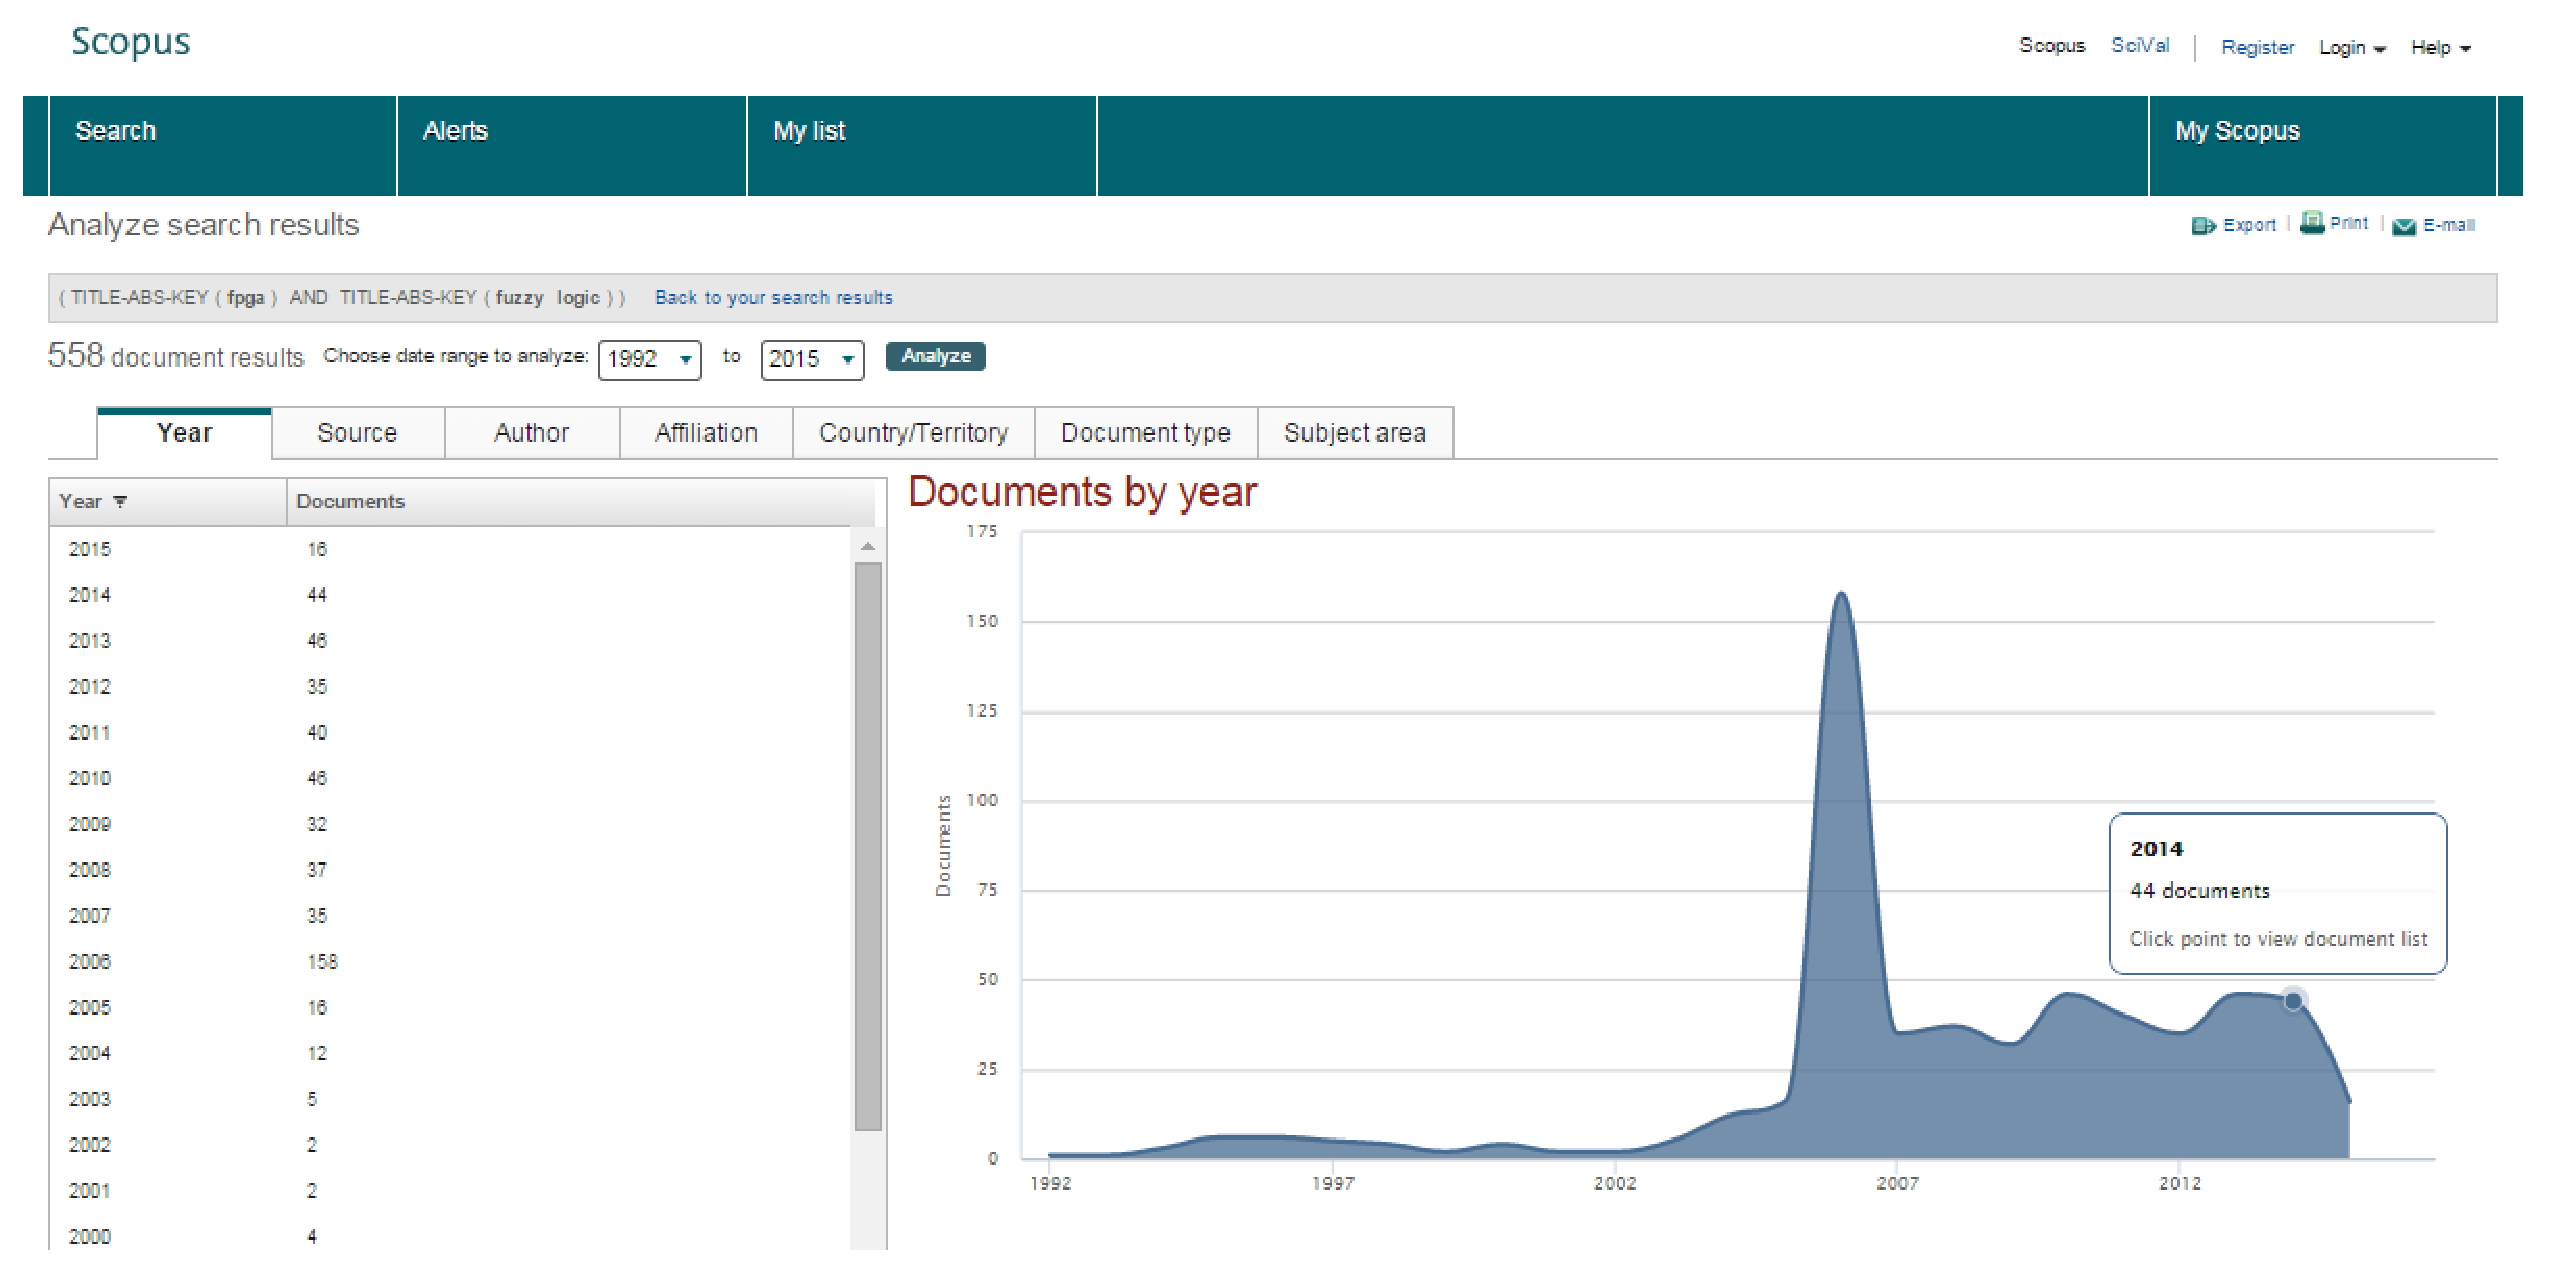
\includegraphics[width=1\linewidth]{Chapter1/chapter1/Fig2_FPGA_trend}
	\caption{Literature on FPGA implementation of FLCS as reported by scopus as on May 2015}
	\label{fig:Fig2_FPGA}
\end{figure}
\begin{figure}[t!]
	\centering
	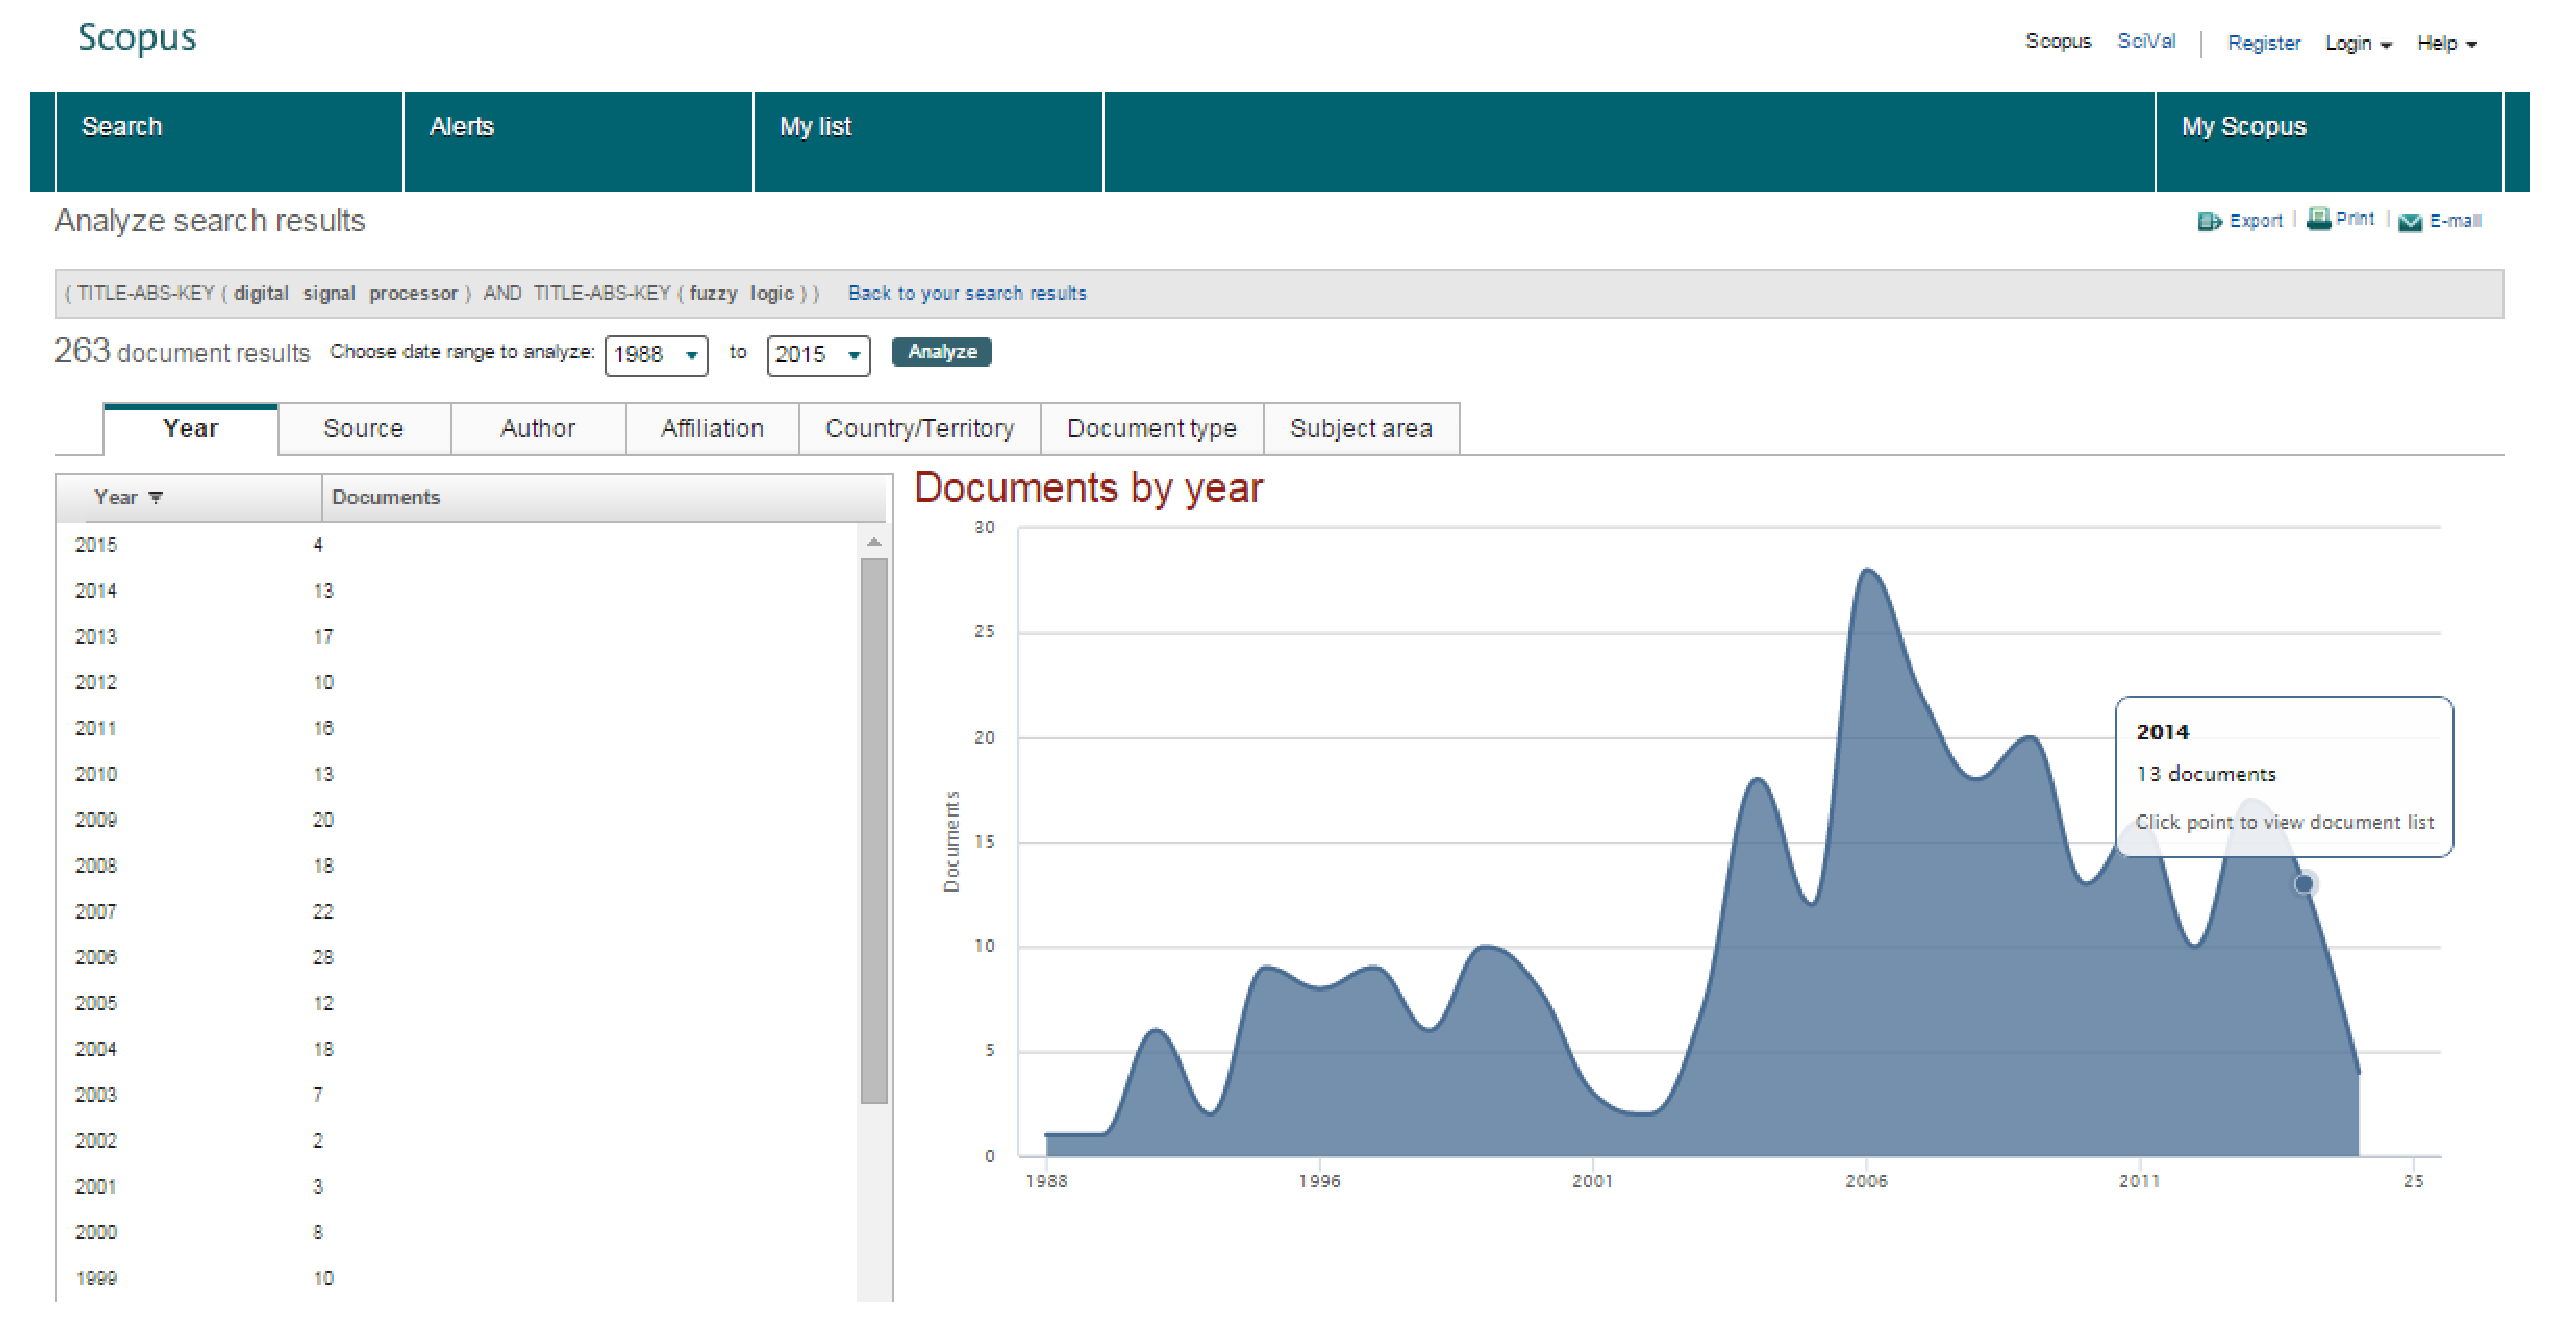
\includegraphics[width=1\linewidth]{Chapter1/chapter1/Fig3_DSP_trend}
	\caption{Literature on DSP implementation of FLCS as reported by scopus as on May 2015}
	\label{fig:Fig3_DSP}
\end{figure}

\subsection{Comparison between various Digital Platform for FLCS Implementation}
It can be seen from Figure \ref{fig:Fig2_FPGA} that FPGA have been most preferred FLCS design platform in literature  \cite{Brox2013,Adhavan2014a,Maji2014a,Messai2011,Tamukoh2007,Schrieber2015,Palakeerthi2014,Santos2014,Benzekri20146109,Islam2013}. Some FLCS architectures have also been developed over an application specific integrated circuit (ASIC) \cite{RoyChowdhury2011,Martinez-Rodriguez2015,Brox2013,Murshid2011,DaijinKim2000} attaining a speed of more than 50 MFLIPS \cite{Bosque2014b,Zavala2012,Murshid2011}. However, the design of these controllers does not make them truly reconfigurable in nature. The major disadvantage is their unavailability for field or on\hyp{}line tuning \cite{Bosque2014b,Passino2010}. It has also been observed that many of the ASIC based designs have been developed using membership function generators (MFGs). MFG circuitry can tune the membership functions (MFs) by setting some voltages on IC pins \cite{Soleimani2014,Mokarram2015} but the Rulebase remains static. To ensure field tunability, it is necessary to impart the FLCS with features that would enable users to change control parameters in run\hyp{}time. In some of the FLCS designs, the fuzzy parameters are stored in digital memory as weights \cite{Bosque2014b,Zavala2012,Kalaykov1999} to impart features of tunability. This technique permits a look-up-table based approach for fuzzy computations which reduces the computation time. However, the online reconfigurability of such system becomes difficult. This technique is well suited for application specific FLCS design where the rulebase and the parameters remain unchanged during the majority of the operation.

Though most of these designs are based on ASIC or FPGA platform, many of the designs are developed on DSP platform for its ease of implementation and reconfigurability \cite{AlNabulsi2012,Kalaykov1999,Mustafa2010,Rubaai2007,Gai2010,Uddin2007,Mohanasundaram201187,wangHuang2013,Maji2013,maji2012design}. From Figure \ref{fig:Fig3_DSP} it is evident that DSP have been also been a preferred platform for implementation of FLCS designs. However, these designs suffer from limitations on the flexibility of weight update. Recently, few RISC processors have included dedicated fuzzy instructions and have been seen to deliver a very high performance in terms of FLIPS \cite{Salapura1998,Watanabe1996,Brox2006,bookGoos2003}. These designs are summarized in Table \ref{tab:survey} where the number of inputs and outputs supported by these systems and maximum number of rules that can be evaluated by these systems is listed. However, the common limitation of many of these designs is that the control parameters can be updated only by removing these controllers from the system, rendering the plant off\hyp{}line. Some of the works have reported to update parameters on\hyp{}line through complex learning processes \cite{Munoz-Salinas2008,Alcala2006,Bandyopadhyay2001a,Boubertakh2010,Demir2011b}. 
In the current decade, DSP based FLCS designs have been widely used in control applications\cite{Heber1997,Butt2004,Suetake2011,Uddin2006}. Over 250 DSP based fuzzy system designs have been reported in last decade according to \url{www.scopus.com}. It has been found that some of the most preferred DSP platforms for this type of design are Texas Instruments' TMS320F series DSPs\cite{Rahmani2013,Pu2014,Eskandarian2014,ElKhateb2014,Okumus2014,Hung2015}, TMS320C series DSPs\cite{Sousa1995,Mustafa2010,Uddin2006,Gai2010,Uddin2007} and dSpace DSPs\cite{MatIsa2012,Noman2013,Rafa2014,Rubaai2007,Butt2004}. The DSP platform is also found to be a preferred platform for FLCS design. 

Even though FPGA is preferred platform for implementation of FLCs compared to a programmable DSP, in this work implementation is done using a TI C6748 DSP processor.  The primary reasons for selection of the mentioned hardware include:
\begin{itemize}
	\item DSP provides efficient implementation of multiplication and accumulation (MAC) and this helps COA implementation.
	\item File handling and socket programming is an integral part of this design. These are achieved easily since the development is done using C language.
	\item This design supports high level of branching and decision making.
\end{itemize}	
Collectively, for this architecture, DSPs were judicially selected over conventional FPGAs. 

\section{Generic Fuzzy Logic Controller}
Generic fuzzy logic controller systems (G\hyp{}FLCS) are standalone and remotely tunable fuzzy logic control devices. These devices are developed on suitable hardware platforms such that they can be easily interfaced with various process plants. The major characteristic of these type of devices is that they do not require reprogramming. These devices accept fuzzy parameters from the users externally through some user interfaces or programmable pins.

\begin{table}[h!]
	\centering
	\caption{Important works on G\hyp{}FLCS}
	\label{tab:survey}
	\resizebox{0.65\textwidth}{!}{%
		\begin{tabular}{llll}
			\hline \noalign{\vskip 2mm}
			Year & \begin{tabular}[c]{@{}l@{}}Speed\\ (in FLIPS)\end{tabular} & Platform & Features \\ \noalign{\vskip 2mm} \hline  \noalign{\vskip 2mm}
			\begin{tabular}[c]{@{}l@{}}1995\\ \cite{Miki1995}\end{tabular} & 0.63M & \begin{tabular}[c]{@{}l@{}}BiCMOS\\ 2$\mu$m\end{tabular} & \begin{tabular}[c]{@{}l@{}}Output MFs: Singleton (7)\\ I/O: 5 bit\\ Input MFs: 11\\ Overlaps: 2\\ Rules Evaluated: 4 per IC\end{tabular} \\ \noalign{\vskip 3mm}  
			\begin{tabular}[c]{@{}l@{}}1996\\ \cite{Watanabe1996}\end{tabular} & 48-122 & \begin{tabular}[c]{@{}l@{}}R3000A \\ RISC\\ Fuzzy \\ Processor\end{tabular} & \begin{tabular}[c]{@{}l@{}}Output MFs: -\\ I/O: -\\ Input MFs: \\ Overlaps: 2\\ Rules Evaluated: 51\end{tabular} \\ \noalign{\vskip 3mm}
			\begin{tabular}[c]{@{}l@{}}2005\\ \cite{Amirkhanzadeh2005}\end{tabular} & 15.87M & \begin{tabular}[c]{@{}l@{}}CMOS\\ 0.35 $\mu$m\end{tabular} & \begin{tabular}[c]{@{}l@{}}Output MFs: Singleton (7)\\ I/O: 2-1\\ Input MFs: 3\\ Overlaps: 2\\ Rules Evaluated: 9\end{tabular} \\ \noalign{\vskip 3mm}
			\begin{tabular}[c]{@{}l@{}}2007\\ \cite{Yosefi2007}\end{tabular} & 16.6M & \begin{tabular}[c]{@{}l@{}}CMOS\\ 0.35 $\mu$ m\end{tabular} & \begin{tabular}[c]{@{}l@{}}Output MFs: Singleton (7)\\ I/O: 2-1\\ Input MFs: 4\\ Overlaps: -\\ Rules Evaluated: 16\end{tabular} \\ \noalign{\vskip 3mm}
			\begin{tabular}[c]{@{}l@{}}2007-2008\\ \cite{Gonzalez2007}\\ \cite{Olivas2008}\end{tabular} & 5.5K & FPGA & \begin{tabular}[c]{@{}l@{}}Output MFs: Singleton (5)\\ I/O: 2-1\\ Input MFs: 8\\ Overlaps: -\\ Rules Evaluated: 64\end{tabular} \\ \noalign{\vskip 3mm}
			\begin{tabular}[c]{@{}l@{}}2010\\ \cite{Fu2010}\end{tabular} & 11K & FPGA & \begin{tabular}[c]{@{}l@{}}Output MFs: - (5)\\ I/O: 2-1\\ Input MFs: 5\\ Overlaps: 2\\ Rules Evaluated: 25\end{tabular} \\ \noalign{\vskip 3mm}
			\begin{tabular}[c]{@{}l@{}}2011\\ \cite{Yosefi2011}\end{tabular} & 16.6M & CMOS & \begin{tabular}[c]{@{}l@{}}Output MFs: Singleton (7)\\ I/O: 2-1\\ Input MFs: 4\\ Overlaps: 2\\ Rules Evaluated:16\end{tabular} \\ \noalign{\vskip 3mm} 
			\begin{tabular}[c]{@{}l@{}}2014\\ \cite{Soleimani2014}\end{tabular} & 15M & \begin{tabular}[c]{@{}l@{}}CMOS\\ 0.35 $\mu$m\end{tabular} & \begin{tabular}[c]{@{}l@{}}Output MFs: Singleton(7) \\ I/O: 2-1\\ Input MFs: 5\\ Overlaps: 2\\ Rules Evaluated:25\end{tabular} \\ \noalign{\vskip 3mm}
			\begin{tabular}[c]{@{}l@{}}2015\\ \cite{Mokarram2015}\end{tabular} & NA & \begin{tabular}[c]{@{}l@{}}CMOS\\ 0.35 $\mu$m\end{tabular} & \begin{tabular}[c]{@{}l@{}}Output MFs: Singleton \\ I/O: 2-1\\ Input MFs: 4\\ Overlaps: 2\\ Rules Evaluated:16\end{tabular} \\ \noalign{\vskip 2mm} \hline
		\end{tabular}
	}
\end{table}

G\hyp{}FLCS designs are mostly crippled by their operational speed and hence they are generally forced to operate under reduced functionalities. Some of the prime G\hyp{}FLCS designs on various platforms have been surveyed and tabulated in Table \ref{tab:survey}. The table also lists the fuzzy parameters reported in these designs. The following observations have been summed up after analyzing these designs. 
\begin{itemize}
	\item It can be observed, that majority of these designs use singleton MFs at the output to reduce computational complexity. Centroid of area (COA) method when applied to singleton, which is commonly known as weighted average defuzzification method yields far low computational complexity. However, unlike COA, weighted average does not compute the area under the curve produced from the fuzzy outputs \cite{Ross2010}. It can be observed that COA presented in eq. \eqref{eq:COA_origin} 
		\begin{equation} \label{eq:COA_origin}
		Y^* = \frac{{\int {{\mu _c}(y)ydy} }}{{\int {{\mu _c}(y)dy} }}
		\end{equation}
	can reduced to weighted average	as depicted in eq. \eqref{eq:wtAvg}.
	\begin{equation}\label{eq:wtAvg}
	{Y^*} = \frac{{\sum {{\mu _c}(y) \cdot y} }}{{\sum {{\mu _c}(y)} }}
	\end{equation}
	where $ Y^* $ represents the crisp output computed from output fuzzy set $ {\mu _c}(y) $ and output support membership function value $ y $.
	\item These designs uses a stringent rule reduction technique where only two overlapping memberships have been considered.
	\item These systems evaluate very few rules to improve computational speed. The reduction in the number of rules with only two overlapping membership functions does not provide desired performance in terms of accuracy of the system for many applications.
	\item In general, these systems cannot be remotely tuned. Some of these devices have MFGs for tuning MFs but the Rulebase remains static and the performance is limited to two inputs. 
\end{itemize} 	
These limitations motivate research in soft\hyp{}core generic FLC devices on programmable hardware where multifarious control over the system can be obtained by varying different control parameters with modest computational complexity.

\section{Problem Statement}
The limitations of the existing G\hyp{}FLCS designs, as defined in Table \ref{tab:survey}, motivated the research in developing a soft\hyp{}core G\hyp{}FLCS device on programmable DSP hardware with two level tuning where multifarious control over the system can be obtained with modest computational complexity. However, this design is extremely challenging owing to following conditions.
\begin{itemize}
\item Since the proposed design is expected to command a large number of fuzzy parameters; it is imperative to develop an interactive interface for guiding users to input fuzzy parameters.
\item It is also a known fact that human beings are prone to make errors while handling large data. Therefore, an automated system has to be deployed which will extract coarse fuzzy parameters from a large input\hyp{}output dataset.
\item The significant challenges in designing such a system lies in managing an exponentially growing rulebase. Therefore, development of a suitable rule reduction technique is required which will generate a desired output consuming minimum cycle time.
\item It has been discussed previously that defuzzification module in FLCS using COA technique is computationally quite expensive. A desirable COA scheme with low computation time is essential to achieving a dependable system cycle time that is relevant to the majority of control applications.
\end{itemize}

\section{Outline of Thesis}
The thesis is presented in 6 chapters. Following this chapter on introduction, the remaining thesis is organized as under:
This thesis is organized as follows:
\begin{itemize}
	\item Chapter 2 presents a mathematical model of the generic fuzzy logic controller and describes the proposed MT\hyp{}FRHC rule reduction technique. A vertices based centroid of area computation algorithm for defuzzification is also proposed.
	\item Chapter 3 explains the design architecture and develops the backbone of the proposed the G\hyp{}FLCS. The proposed architecture includes a web based user interface (WebUI) for users to program fuzzy parameters in  the GFLCS, a genetic algorithm based fuzzy parameter extraction scheme and a fuzzy framework.
	\item Chapter 4 implements the concepts developed in Chapter 2 and 3 in optimized C code and realizes the proposed G\hyp{}FLCS on a C6748 DSP processor. Applicability and performance analysis of the G\hyp{}FLCS is analyzed.
	\item In Chapter 5, the proposed G\hyp{}FLCS is used to control the radial position of plasma in Aditya Tokamak Fusion Test Reactor (TFTR). The GA based fuzzy parameter extraction process is used to obtain FCP for the control problem. This FCP is used to control the plasma position in the Aditya TFTR Simulink model and the same is compared to some of the previously developed systems.
	\item Finally the research work is concluded in chapter 6 and the scope of future work is explained briefly. The limitations and the scope for future work of this research are also elaborated in this chapter.
\end{itemize}


\chapter{Generic Fuzzy Logic Controllers}
\begin{chapterAbstract}{Preview}
This chapter presents an introduction to mathematical deduction of G\hyp{}FLCS architecture. A rule reduction scheme compatible with this architecture is also incorporated to reduce the complexity of the system and assure it is realizable in real-time. The proposed scheme is called modified and thresholded fired rules hyper cube (MT-FRHC), and it is based on rule reduction technique using overlapping membership functions. In MT-FRHC, control designers can dynamically assign the number of overlaps to be considered within the G\hyp{}FLCS system. Further, a thresholded fuzzifier optimizes the system with discourse to computational complexity and throughput accuracy. In the proposed system architecture, the number of t-norm and t-conorm operations per inferences can also be dynamically varied between discrete values. This fuzzy model is analyzed with the context of its output performance and computational complexity. A formative observation in favour of MT-FRHC has been inferred from this analysis.
\end{chapterAbstract}
\clearpage

\section{Introduction to Generic Fuzzy Logic Controller System} \label{sec:ch2-GFLC}
\par
G\hyp{}FLCS are essentially hardware based general purpose control devices operating on fuzzy logic principles. Characteristic features of these control devices include
\begin{itemize}
	\item Plug and play framework,
	\item Runtime tunability, and
	\item Standalone operation.
\end{itemize}
\par
In this chapter, a G\hyp{}FLCS is presented that provides a runtime reconfigurable framework. This fuzzy system can be employed to control any system that is in tandem with the controller I/O specifications. In most G\hyp{}FLCS designs, fuzzy control parameters (FCP) are updated as weights. FCP defines the parameters like number of Inputs and Outputs, number of MFs in each Input and Output, details of each MF like, their function type and their co-ordinates, the Rulebase of the FLC defined by the index numbers of the inputs and outputs. These parameters are put into a FLC framework that drives the operation of the fuzzy system. However, it can be noted that not all FCPs in a G\hyp{}FLCS are updated at run-time. The parameters that can be updated at run-time depends on the architecture of G\hyp{}FLCS, and can be termed as \textit{flexible parameters} of G\hyp{}FLCS. Yosefi et. al. \cite{Yosefi2007,Yosefi2011} implemented G\hyp{}FLCS on 0.35 $ \mu $m CMOS technology to achieve 16.6 MFLIPS but used singleton type membership functions at the output with a rigid Rulebase. Moreover, only two overlapping membership functions are considered in the design. Vasantha Rani et. al. \cite{VasanthaRani2005} introduced multicycle architecture for G\hyp{}FLCS and implemented it on FPGA to achieve an operational speed of 31K FLIPS. This system used singleton membership functions at the output. It also used reduction in the number of rules that can be accommodated. Most FLC designs in literature, are developed on reconfigurable hardware namely FPGAs \cite{Messai2011a,Brox2013,Adhavan2014a}. Some of these have also been developed on application specific integrated circuit (ASIC) and have attained a speed of more than 50 MFLIPS \cite{Bosque2014b,Zavala2012}. But it can be observed among these G\hyp{}FLCS designs that, the majority of FCPs are not recognized as flexible parameters and programmed directly into FLC core to achieve high speed. This leads to conclusion that, the computational complexity of a G\hyp{}FLCS system depends on,
\begin{itemize}
	\item Number of FCPs considered as flexible parameters in the G\hyp{}FLCS  design;
	\item Maximum number of rules that the G\hyp{}FLCS can accommodate,
	\item The type of defuzzification method employed for the conversion of the output from fuzzy domain to crisp real value.
\end{itemize}
\par
Some of the commonly used defuzzification methods include, centroid of area (COA), bisector of area (BOA), mean of maxima (MOM), largest of maxima (LOM) and smallest of maxima \cite{Ross2010}. COA is one of the most commonly used defuzzification method in control applications and implemented as \cite{Grigorie2011}.
\begin{equation} \label{eq:COA}
Y^* = \frac{{\int {{\mu _c}(y)ydy} }}{{\int {{\mu _c}(y)dy}}}
\end{equation}
where $ Y^* $ represents the crisp output computed from output fuzzy set $ {\mu _c}(y) $ and output support membership function value $ y $. 
However, COA is highly resource intensive when fuzzy set associated with the output consists of fuzzy numbers of type other than singleton. For singleton type output fuzzy set the continuous representation in \eqref{eq:COA} is reduced to discrete representation leading to \cite{Ross2010} 
\[{Y^*} = \frac{{\sum {{\mu _c}(y) \cdot y} }}{{\sum {{\mu _c}(y)} }}\]
This chapter introduces a novel rule reduction technique named as MT-FRHC. It improves the accuracy of existing overlap based rule reduction technique. Fast inference time is the most important feature of the overlapping MFs based rule reduction technique. The proposed MT-FRHC system achieves to increase the accuracy without increasing the inference time. The FRHC rule reduction algorithms which is widely accepted and used because, it is the only algorithm which performs effective rule selection without pruning or forking into the Rulebase provided from the user \cite{Razib2013,Munoz-Salinas2008,Alcala2006,Sanz2011}. Pruning and forking of rules in original rulebase is an application specific process \cite{Nguyen2015,Wang1992a,Setnes1998}. These type of rule reduction techniques are not suitable for generic fuzzy systems. Pruning and forking of rules can be applied as a wrapper on top of the proposed G-FLCS but these methods cannot be programmed into the core of the G-FLCS. There are also layer-structured machine learning algorithms (Neural Network, Genetic Algorithm) to learn the effective rules \cite{Shann1995,Ishibuchi1995,Ishibuchi1995a}. However, these methods for rule extraction are computationally quite expensive. Thus when an application is known, the fuzzy control parameters (which include rulebase) can be extracted using these techniques. These techniques provide good default parameters and this is described in Chapter 5 elaborately. For implementation of G-FLCS in radial position control of plasma in Aditya TFTR, a genetic algorithm based rule extraction technique is used which reduces the rules in rulebase and thereby reducing effective rules. Therefore, it was required to derive an effective rule reduction scheme that do not fork and prune the original rulebase like FRHC. Therefore, in this work, the FRHC algorithm has been mathematically analyzed and suitable assumptions have been introduced in it which can dynamically control the computational complexity of the G-FLCS based on user requirement. 

\subsection{Rule Reduction using Overlapping Membership Functions}
The concept of overlapping membership functions has been widely used in reducing computational time of fuzzy systems, specially in hardware development of FLC as it eradicates the non-linear dependency between number of inputs and computational complexity in the G\hyp{}FLCS. It was originally proposed by Eichfled et. al. in 1992 \cite{Eichfeld1992} and it was improvised in 1999 by I. Kalaykov and named as Fired-Rules-Hyper-Cube (FRHC) \cite{Kalaykov1999}. However, this rule reduction method is constrained by anticipating fixed number of overlaps that can affect controller performance. It is characterized by a layered parallel architecture of the fuzzy inference. Moreover, it reduces the dependency of processing time on the number of inputs to the fuzzy system while dependency on the number of rules and fuzzy partitioning of all variables are completely eradicated. This concept has been adopted in various implementations of FLCS resulting in enhancement of speed \cite{Razib2013,Munoz-Salinas2008,Alcala2006,Sanz2011}.  However, this stipulation of segregation of input space with maximum of two overlapping membership functions, causes major bottleneck in accuracy and tuning of the FLC, specially because the MFs cannot be unevenly distributed over the input spaces, which is seen to be circumstantial in majority of non-linear FLC system design. However, if employed in control of a non-linear system where the MFs are unevenly distributed over the input space, this technique of rule reduction would fail to provide expected accuracy.

\subsection{Motivation for Modified FRHC (M-FRHC)} \label{sec:RLB:MFRHC}
FRHC rule selection method constraints the Rulebase design by limiting the number of MFs operating over any part of the input region to two. But when this algorithm is applied to higher order non-linear systems with uncertainties, the system performance gets affected and tuning becomes extremely difficult \cite{Alcala2006a,Alcala2006}. Fuzzy controllers are important in situations where large uncertainties or unknown variations are predominant in parameters and structures of a plant. By introducing FRHC, this essence of Fuzzy Control is lost to certain extent because of the assumption that only two overlapping membership operates over the solution space. It is not sufficient to create a fuzzy hypothesis which can incorporate large uncertainty and unknown variations. But, at same instance, FRHC based G-FLCS is computationally cheap and easy to implement.

The most important module in the tuning of G-FLCS is the learning of FCP, that can be achieved by many algorithms, namely Genetic Algorithm (GA), Univariate Marginal Distribution Algorithm (UMDA) and others. The convergence of these optimization algorithms depend on the flexibility of the membership functions and the fuzzy partitioning of the input and the solution space. Since FRHC is a constraint based rule reduction scheme, the convergence of the optimization algorithms are subject to the complexity of the system. This implies that the convergence may or may not occur for a fairly complex system. Therefore, it is the modality of the rule reduction scheme that needs to refined in accordance to the proposed G-FLCS. 

Thus to keep the simplicity of the FRHC intact while countering its limitations of flexibility and modality, a modified fired-rules-hyper-cube (M-FRHC) rule reduction technique is proposed and incorporated.
\begin{figure}[ht]
	\centering
	\includegraphics[width=0.85\linewidth]{Chapter2/chapter2/Antecedent_3.eps}
	\caption{More than two fuzzy logic antecedent membership functions overlapping at once}
	\label{fig:FuzzyLogicAntecedentMembershipFunctions}
\end{figure}

Advantages of the proposed M-FRHC over its conventional counterpart FRHC, can be understood considering a case where fuzzy logic antecedent MFs are distributed in the input space as shown in Figure \ref{fig:FuzzyLogicAntecedentMembershipFunctions}. In the input space marked as $ X $ and $ Y $, any crisp input shall be fuzzified to more than two non-zero membership grade since there are more than two overlapping MFs. It is observed that the number of non-zero membership grade in a fuzzified input cannot exceed more than the maximum number of overlaps between the MFs distributed in the input space. In systems where optimization of FCPs are implemented, it is more often than not that the MFs in the input, as well as in the output space, will be distributed unevenly, and their overlaps will be inconsistent. When FRHC is applied on these set of input MFs, useful data is lost if crisp input lies within X or Y region of the input space. FRHC algorithm will fire the first two rules related to the non-zero fuzzy values instead of three rules which is evident. This process is potentially erroneous where the error in the control output is proportional to the weights of the membership function(s) discarded and its associative implication on the Rulebase. Implementation of M-FRHC will allow the number of overlaps to vary suitable with conjunction to the complexity of the control system. 

M-FRHC operates on a platform of dynamical assertion of overlaps in membership functions as per the Table \ref{tab:ch2NCells}. Based on the number of inputs, M-FRHC will dynamically controls the number of overlaps to be considered. Introduction of this feature allows fuzzy model to be flexible enough to accommodate the uncertainties and modality of the system. However, with increase in input, when there is an exponential growth in computational complexity, it reduces the overlaps that are considered to reduce the computational complexity. This enforces a trade off between accuracy and speed. However, in truly generic systems, the operating point of this trade off should be defined by user. M-FRHC introduces a sophisticate approach to achieve this through the concept of $N_{Cells}$ which defines the operating point on the accuracy and speed trade off. It is to be noted that in Table \ref{tab:ch2NCells}, the bold and underlined values of $N_{Cells}$ are used for all experiments appearing in later part of this thesis. Although, it remains in the discretion of the user to use any values of $ N_Cells $ for a given $ O $ and $ n $. 

For example, consider the following rules,
\[\begin{array}{l}
If~input~I~is~M{F_1}~then~Output~O~is~{P_1}\\
If~input~I~is~M{F_2}~then~Output~O~is~{P_2}\\
If~input~I~is~M{F_3}~then~Output~O~is~{P_3}
\end{array}\]
and the membership distribution over input space be as in Figure \ref{fig:FuzzyLogicAntecedentMembershipFunctions}. For an input value assuming to be 20, the actual fuzzication output will be approximately,
\[M{F_1} = 0.4,~M{F_2} = 0.5,~M{F_3} = 0.2\]
FRHC under the assumption of two overlapping membership function will return,
\[M{F_1} = 0.4,~M{F_2} = 0.5\] 
which implies that rule number three does not fire. However, the system expects rule three to fire since it has a weight of 0.2 associated with membership function $P_3$ in the output or solution space. In retrospective, if $N_{Cells}$ is configured to 5 with with number of inputs being one, M-FRHC will consider maximum number of five overlaps in the membership function. Hence, it will generate 
\[M{F_1} = 0.4,~M{F_2} = 0.5,~M{F_3} = 0.2\]
ass the system would expect and thus firing rule number three in the Rulebase.

\subsection{Analytical Differences between Conventional Overlapping Membership Function (OMF) method and M-FRHC}
FRHC based rule reduction scheme uses the concept of two overlapping membership functions to reduce the computation. This method is valid when the maximum number of overlapping MFs distributed over the input space is limited to two. However, to counter uncertainty and variations in a nonlinear plant, adaptive control is imperative. The basic objective of an adaptive control strategy is to maintain smooth performance of a system in the presence of these uncertainties. Therefore, introduction of online and offline adaptive fuzzy control is important feature of a G-FLC which essentially means updating and tuning FCP at various time intervals. The implementation of adaptive fuzzy control strategy in proposed G-FLCS is explained in Chapter 3. So, with M-FRHC in operation, the uncertainties are modeled better compared to conventional overlapping membership methods of active rule reduction.   

In FRHC technique, \cite{Kalaykov1999,Eichfeld1992}
\begin{align} \label{eq:FRHC_main}
y&= y_{aggr}.\left ( y_{w}^{-1} \right ) \\
\text{where}\\ \nonumber
y_{aggr}&=\sum_{i=1}^{N_{cells}} w_{i}.y_{i} \text{,} y_{w}&=\sum_{i=1}^{N_{cells}} w_{i} \nonumber 
\end{align}
where $ w_{i} $ represents the non-zero weights of the fuzzified input and $ y_{i} $ represents the \textit{Kernel} of a output fuzzy set fired by the Rulebase. 

\begin{Definition}[Fuzzy Set]\label{def:fSet} 
Let $ X $ be a nonempty set. A \emph{fuzzy set} $ A $ in $ X $ is characterized by its MFs.
\[{\mu _A}:X \to \left[ {0,1} \right]\]
and $ {\mu _A}(x) $ is interpreted as the degree of membership of element $ x $ in fuzzy set $ A $ for all $x \in X$.
\end{Definition} 

\begin{Definition}[Kernel or Core]\label{def:kernel} 
	Let $ A $ be a fuzzy subset of $ X $; the support of $ A $, denoted $ supp(A) $, is the crisp subset of $ X $ whose elements all have nonzero membership grades in $ A $.
	\[core\left( A \right) = \left\{ {x \in X|A\left( x \right) = 1} \right\}\]
\end{Definition} 

\begin{Definition}[Support]\label{def:suppSet} 
	Let $ A $ be a fuzzy subset of $ X $; the support of $ A $, denoted $ supp(A) $, is the crisp subset of $ X $ whose elements all have nonzero membership grades in $ A $.
	\[supp\left( A \right) = \left\{ {x \in X|A\left( x \right) > 0} \right\}\]
\end{Definition} 

\begin{table}[h!]
	\caption{Computed $N_{cells}$ with varying $n$ and $O$}
	\label{tab:ch2NCells}
	\centering
	\begin{tabular}{rrrrr}
		\hline \noalign{\vskip 1mm} 
		&       $  n=1 $ &        $ n=2 $ &        $ n=3 $ &        $ n=4 $ \\
		\hline \noalign{\vskip 1mm} 
		$ O=2 $ &          2 &          4 &          8 &         \textbf{\underline{16}} \\ \noalign{\vskip 2mm}
		
		$ O=3 $ &          3 &          9 &         \textbf{\underline{27}}&         81 \\ \noalign{\vskip 2mm}
		
		$ O=4 $ &          4 &         \textbf{\underline{16}}&         64 &        256 \\ \noalign{\vskip 2mm}
		
		$ O=5 $ &          \textbf{\underline{5}} &         25 &        125 &        625 \\\noalign{\vskip 2mm}
		
		$ O=6 $ &          6 &         36 &        216 &       1296 \\ \noalign{\vskip 2mm}
		
		\textbf{M-FRHC} &          \textbf{\underline{5}} &        \textbf{\underline{16}} &         \textbf{\underline{27}} &         \textbf{\underline{16}} \\
		\hline
	\end{tabular} 
\end{table}

Most G-FLCS are designed on the principles described in \eqref{eq:FRHC_main}. For all such FLCs, it can be observed that the computational complexity depend on $ N_{cells} $ which is non-linearly related to number of overlapping membership functions and number of system inputs. The number of system inputs can be presented as:
\begin{equation} \label{eq:ncells}
N_{cells} = {O}^n
\end{equation}
where, $O$ represents the number of overlaps considered and $n$ represents the number of inputs. The values of $ N_{cells} $ for different $O$ and $ n $ is computed and tabulated in Table \ref{tab:Nops}. This shows that $ N_{cells} $ increases exponentially with respect to the $ n $. This dependency of $ N_{cells} $ on $ O $ and $ n $ can be analyzed for the Table \ref{tab:Nops}. For system implementation FRHC is a popular choice, where $ O = 2 $ as \cite{Kalaykov1999} states that, ``..uncertainty has to be on boundary between two fuzzy sets". Hereby, FRHC will take values from first column of Table \ref{tab:ch2NCells} depending on the in the system inputs. Now, if $O$ predefined, the generic FLC system assumes value of $ N_{cells} $ based on $n$ and this remains static. Additionally, the computational complexity increases exponentially with increase in $n$. 

Consider a fuzzy logic system with $ n $ inputs where each input have $ x $ numbers of membership functions. This implies that the number of rules that can result from this combination is $ x^{n} $. Now, for any input value $I = \left[ {{i_1},{i_2},{i_3}...{i_n}} \right]$, the resultant vectors $ \left\{ {\Psi ({i_p}),\forall p \in \left[ {1,n} \right]} \right\} $ (fuzzified inputs) will have maximum of $ O $ numbers of non-zero values, where $ O $ is the maximum number of overlapping membership functions distributed over each of the input space. The number of effective or active rules that can be fired will only depend on number of non-zero values in the resultant fuzzified input. The number of non-zero values are directly proportional to the number of overlaps as shown in region $ X $ and $ Y  $ in Figure \ref{fig:FuzzyLogicAntecedentMembershipFunctions}. It can be observed that, $ O^{n} $ out of a set of $ x^{n} $ possible rules will be effective rules. $ N_{cells} $ represents the number of active rules in FRHC rule reduction scheme.

In the proposed MT-FRHC system, the maximum number overlapping membership functions considered at inference can be dynamically varied to provide computational advantage. To strike a balance between accuracy and computational complexity, it is important to control the maximum number of overlapping membership functions dynamically. In this G-FLCS implementation, the maximum number of overlaps to be considered has been systematically reduced with increase in the number of inputs. With increase in the number of inputs, number of rules in an FLC increases exponentially leading to increased computational complexity. However, this exponential growth in computational complexity can be curtailed by decreasing the number of overlaps.

It can be noted that, in MT-FRHC the values of $ N_{cells} $ can be assumed from Table \ref{tab:ch2NCells} randomly. However, the proposed MT-FRHC scheme allow us to dynamically choose the maximum number of overlapping membership functions which are underlined in Table \ref{tab:ch2NCells}. It can be observed that the assumed values appear as diagonal elements of Table \ref{tab:ch2NCells}. This is a naive approach to implement the concept that as the number of inputs increases, the maximum number of overlaps to be considered decreases.
As, $N_{cells} = {O^n}$ implies that $O = \sqrt[n]{{N_{cells}}}$. Again, $ N_{cells} $ is directly proportional to computational complexity as shown in \eqref{eq:FRHC_main}.
To achieve a constant $ N_{cells} $, $ O $ should be varied in accordance to the change in number of input $ n $. Thus in this G-FLCS implementation, $ \forall n = \left\{ {1,2,3,4} \right\} $, $ O={5,4,3,2} $. Using these values in \eqref{eq:ncells}, in the proposed M-FRHC based G-FLCS design, $ N_{cells} $ are assumed as following 
\begin{align}
N_{cells} = \left\{\begin{matrix}
5,~\forall n = 1\\ 
16,~\forall n = 2\\ 
27,~\forall n = 3\\ 
16,~\forall n = 4
\end{matrix}\right. \nonumber
\end{align} 
These values of $ N_{cells} $ are assumed such that the number of effective rules for every inference could be kept low without affecting the accuracy of the system. This combination is seen to be optimal for this system since, increasing the number of inputs will have minimum effect on overall computation time and complexity. 

In summary, for any system where MFs are distributed randomly over the input space (as shown in an example Figure \ref{fig:FuzzyLogicAntecedentMembershipFunctions}), FRHC will fail to produce desired control output. However, configuring $N_{Cells}$ effectively, M-FRHC can tackle the evenness in the distribution of the fuzzy memberships in the input and the solution space. The flexibility and modality of the M-FRHC algorithm is completely tunable and hence it provides more inclusive environment for tuning and optimization of FCP using learning algorithms. Due to the flexibility in the structure, M-FRHC can generate complex hypothesis for FCP to incorporate large uncertainties and variations. Thus in these applications, FRHC can be replaced by proposed M-FRHC as the rule reduction technique and tuned accordingly for improved performance and accuracy. 

\section{Mathematical Modeling of G\hyp{}FLCS} \label{sec:ch2-mathmod}

\begin{Lemma}[Vector Combination]\label{lem:VecComb} 
	Let $ A $ and $ B $ be two vector of dimension $ d $. 
$ \Lambda_c (A,B)$ returns a matrix $ M $ of dimension $ d^2\times2 $. 
\[{\textbf{m}_{i,j}} = \left( {{a_i},{b_j}} \right)\forall i,j \to [1,d]\]
where,\\
$ {\textbf{m}_{i,j}} $ represents individual row in matrix $ M $ and consists of two elements $ a_i $ and $ b_j $ each from set A and B respectively. 
\end{Lemma} 

A multiple-input single-output (MISO) FLCS with $ N $ number of inputs is considered. Each input space is segregated in $ z_j $ fuzzy numbers and $ M $ represents the maximum number of membership functions that the system can accommodate. The set of fuzzy numbers spread over each input space can be presented as

%\[Z = \left\{ {{z_j}} \right\} \text{ where } {z_j} \in [1,M]~\forall j = \left\{ {1,2, \ldots N} \right\}\]
\[Z = \left\{ {{z_j}|{z_j} \in [1,M],\forall j \to \left[ {1,N} \right]} \right\}\]

The FLCS transform the crisp inputs to the fuzzy domain using a \textit{fuzzifier} module. If input $ i $ is introduced to the \textit{fuzzifier} with $ M $ membership functions, then \textit{fuzzifier} module returns a set of values corresponding to degree of each membership when input $ i $ is mapped on them. This can be represented as 
\begin{equation} \label{eq:gamma}
\Delta  \left( i \right) = \psi _i  = \left\{ {\mu _1 \left( i \right),\mu _2 \left( i \right), \ldots \mu _M \left( i \right)} \right\}
\end{equation}
where $ \left\{ {{\mu _j}\left( i \right) \in \left[ {0,1} \right],\forall j \to [1,M]} \right\} $
\par		
Input vector $ I = \left \{ i_{1}, i_{2} \cdots i_{N}\right \} $ is a set of scalar inputs, also known as crisp input, to the FLCS system. When $ I $ is introduced to \textit{fuzzifier} module it is transformed to fuzzy domain as shown in \eqref{eq:Ftran}. 

\begin{equation} \label{eq:Ftran}
\Delta  \left( I \right) = \left[ {\begin{array}{*{20}{c}}
	{{\psi _1}}\\
	{{\psi _2}}\\
	\vdots \\
	{{\psi _N}}
	\end{array}} \right] = \left[ {\begin{array}{*{20}{c}}
	{{\mu _1}\left( {{i_1}} \right)}&{}& \ldots &{{\mu _M}\left( {{i_1}} \right)}\\
	{{\mu _1}\left( {{i_2}} \right)}&{}& \ldots &{{\mu _M}\left( {{i_2}} \right)}\\
	\vdots &{}& \vdots & \vdots \\
	{{\mu _1}\left( {{i_N}} \right)}&{}& \ldots &{{\mu _M}\left( {{i_N}} \right)}
	\end{array}} \right]
\end{equation}


$ \Lambda_c $ is vector combination function operated on $ \Delta  \left( I \right)  $ to generate $ {C_R} $, a matrix of size $ \left( {{M^N} \times N} \right) $.
\[{C_R} = {\Lambda_c}{\left( {{\psi _1},{\psi _2}, \cdots {\psi _N}} \right)'}\]

If a Rulebase matrix $ R_b $ with $ N_R $ rules is sorted based on antecedent, then each set of antecedents corresponds to the index of consequent. A generalized structure of a rule in Mamdani FLCS can be represented as,

$ k^{th} $ Rule:
\begin{equation} \label{eq:a_c}
{R_b}\left( k \right):~~~~\text{If}~i_1\text{ is }{a_{1,k}}~\text{and}~i_2\text{ is }{a_{2,k}}~\text{and}~\cdots \text{and}~i_N\text{ is }{a_{N,k}},~\text{then}~{c_j}
\end{equation}
where, antecedents $ {a_1},{a_2} \cdots {a_N} $ can be represent a unique index $ k $, and $ k $ is represented by 
\begin{equation} \label{eq:index}
k = {\left( {{a_N}{a_{N - 1}} \cdots {a_0}} \right)_M} = \sum\limits_{j = 0}^N {{a_j}{M^j}} 
\end{equation}
where, $ M $ represents the maximum number of membership functions and $ N $ repesents the number of inputs with  $ j \to [1,N]$.
Therefore, the $ k^{th} $ index in Rulebase matrix points to corresponding consequent.
\begin{equation}
{R_b}\left( k \right) = {c_j}
\end{equation}
where $ {c_j} \in \left[ {1,M} \right]~\forall j = \left\{ {1,2, \ldots {N_R}} \right\} $

The fuzzy output inferred from Rulebase is a fuzzy set $ \theta_f $ which is essentially a vector of $ M $ elements.

\begin{equation} \label{eq:out_rel}
{\theta _f}({c_j}) = \bigcap\limits_{k = 0}^{{N_R} - 1} {\left( {{\theta _f}\left( {{R_b}\left( k \right)} \right),\left( {\bigcup\limits_{l = 0}^{N - 1} {\overrightarrow {{C_R}\left( l \right)} } } \right)} \right)} 
\end{equation}
where, $ {\theta _f} $ is  fuzzy output vector, index $ k $ varying from $ 0  $ to number of rules $ N_R $, $ R_b $ is the rule base matrix, $ C_R $ represents the vector combination of fuzzified input, $ l $ varying from $ 0 $ to $ N-1 $ and $ \bigcap {} $  and $ \bigcup {} $ representing t-norm and s-norm operations respectively.
The \textit{defuzzifier} in G-FLCS converts fuzzy output vector $ {\theta _f} $ into scalar output commonly known as crisp output. 
\begin{align}	\label{eq:InvOperator}	
{\theta _f} &= \left\{ {{\mu _1}\left( \theta  \right),{\mu _2}\left( \theta  \right), \ldots {\mu _M}\left( \theta  \right)} \right\} \nonumber \\
\theta  &= {\Delta  ^{ - 1}}\left( {{\theta _f}} \right)
\end{align}
where, $ {\Delta  ^{ - 1}} $ denotes inverse fuzzy operator operating on fuzzy output vector $ {\theta _f} $.

\subsection{Overlapping Membership based Rule Reduction}
FRHC can be realized by considering $ M=2 $ in \eqref{eq:Ftran}. To implement this, the index of corresponding non-zero membership functions needs to be pursued and used during inference mechanism. It is recorded in a matrix $ P_{i} $. Thus, for this condition \eqref{eq:gamma} can be represented as

\[\Delta  \left( i \right) = {\psi _i} = \left\{ {\begin{array}{*{20}{c}}
	{\left\{ {{\mu _1}\left( i \right),{\mu _2}\left( i \right), \ldots {\mu _M}\left( i \right)} \right\}}\\
	{\left\{ {{p_1}\left( i \right),{p_2}\left( i \right), \ldots {p_M}\left( i \right)} \right\}}
	\end{array}} \right.\]

Now, replacing $ M = 2 $, \eqref{eq:Ftran} becomes,
\begin{equation} \label{eq:FRHC_O}
\begin{array}{*{20}{c}}
{\psi _I} = \left[ {\begin{array}{*{20}{c}}
	{{\mu _1}\left( {{i_1}} \right)}&{}&{{\mu _2}\left( {{i_1}} \right)}\\
	\vdots &{}&{}\\
	{{\mu _1}\left( {{i_N}} \right)}&{}&{{\mu _2}\left( {{i_N}} \right)}
	\end{array}} \right] \\~ \\
{P_I} = \left[ {\begin{array}{*{20}{c}}
	{{p_1}\left( {{i_1}} \right)}&{}&{{p_2}\left( {{i_1}} \right)}\\
	\vdots &{}&{}\\
	{{p_1}\left( {{i_N}} \right)}&{}&{{p_2}\left( {{i_N}} \right)}
	\end{array}} \right]
\end{array}
\end{equation}
where $ {\psi _I} $ represents fuzzified input matrix with non-zero membership degree and $ P_I $ represents the index of these non-zero membership degree. 

\[\begin{array}{l}
{C_{{R_k}}} = {\Lambda _c}\left( {{P_1},{P_2}, \ldots {P_N}} \right)\\
{C_{{R_V}}} = {\Lambda _c}\left( {{\psi _1},{\psi _2}, \ldots {\psi _N}} \right)
\end{array}\]
Thus, the vector combination operation is to be applied on both matrices, $ P_I $ and $ \psi _I $ to obtain resultant matrices $ {C_{{R_k}}} $ and $ {C_{{R_V}}}  $.
With this the output relationship \eqref{eq:out_rel} can be represented as
\begin{equation} \label{eq:FRHC-final}
{\theta _f}({c_j}) = \bigcap\limits_{{k_x} = 0}^{({N^{{2}}) } - 1} {\left( {{\theta _f}\left( {{R_b}\left( {{k_x}} \right)} \right),\left( {\bigcup\limits_{l = 0}^{N - 1} {\overrightarrow {{C_{{R_V}}}\left( l \right)} } } \right)} \right)} 
\end{equation}
where $ {\theta _f} $ is  fuzzy output vector, index $ k_x $ varying from $ 0  $ to number of rules $ (N^{O_l} - 1) $, $ R_b $ is the rule base matrix, $ C_{R_V} $ represents the vector combination of non-zero fuzzified input values, $ l $ varying from $ 0 $ to $ N-1 $ and $ \bigcap {} $  and $ \bigcup {} $ representing t-norm and s-norm operations respectively.

\subsection{Modified Fired Rulebase Hyper Cube (M-FRHC)}
The G\hyp{}FLCS described earlier in this section, has a complexity of $ \mathcal{O}\left( {{M^N}} \right) $. For FRHC rule reduction technique $ M = 2 $, the computational complexity reduces to $ \mathcal{O}\left( {{2^N}} \right) $. Table \ref{tab:Nops} presents the relationship between and number of overlaps considered, with reference to number of Inputs. The complexity $ \mathcal{O} $ is proportional to number of operations per fuzzy inference $ n_{op}  $. Therefore these notions can be cumulatively formulated as

\begin{equation} \label{eq:overlap}
{n_{op}} = {O_l}^N
\end{equation} 
where $ O_l $ is the number of overlaps considered. 

\begin{figure}[h!]
	\centering
	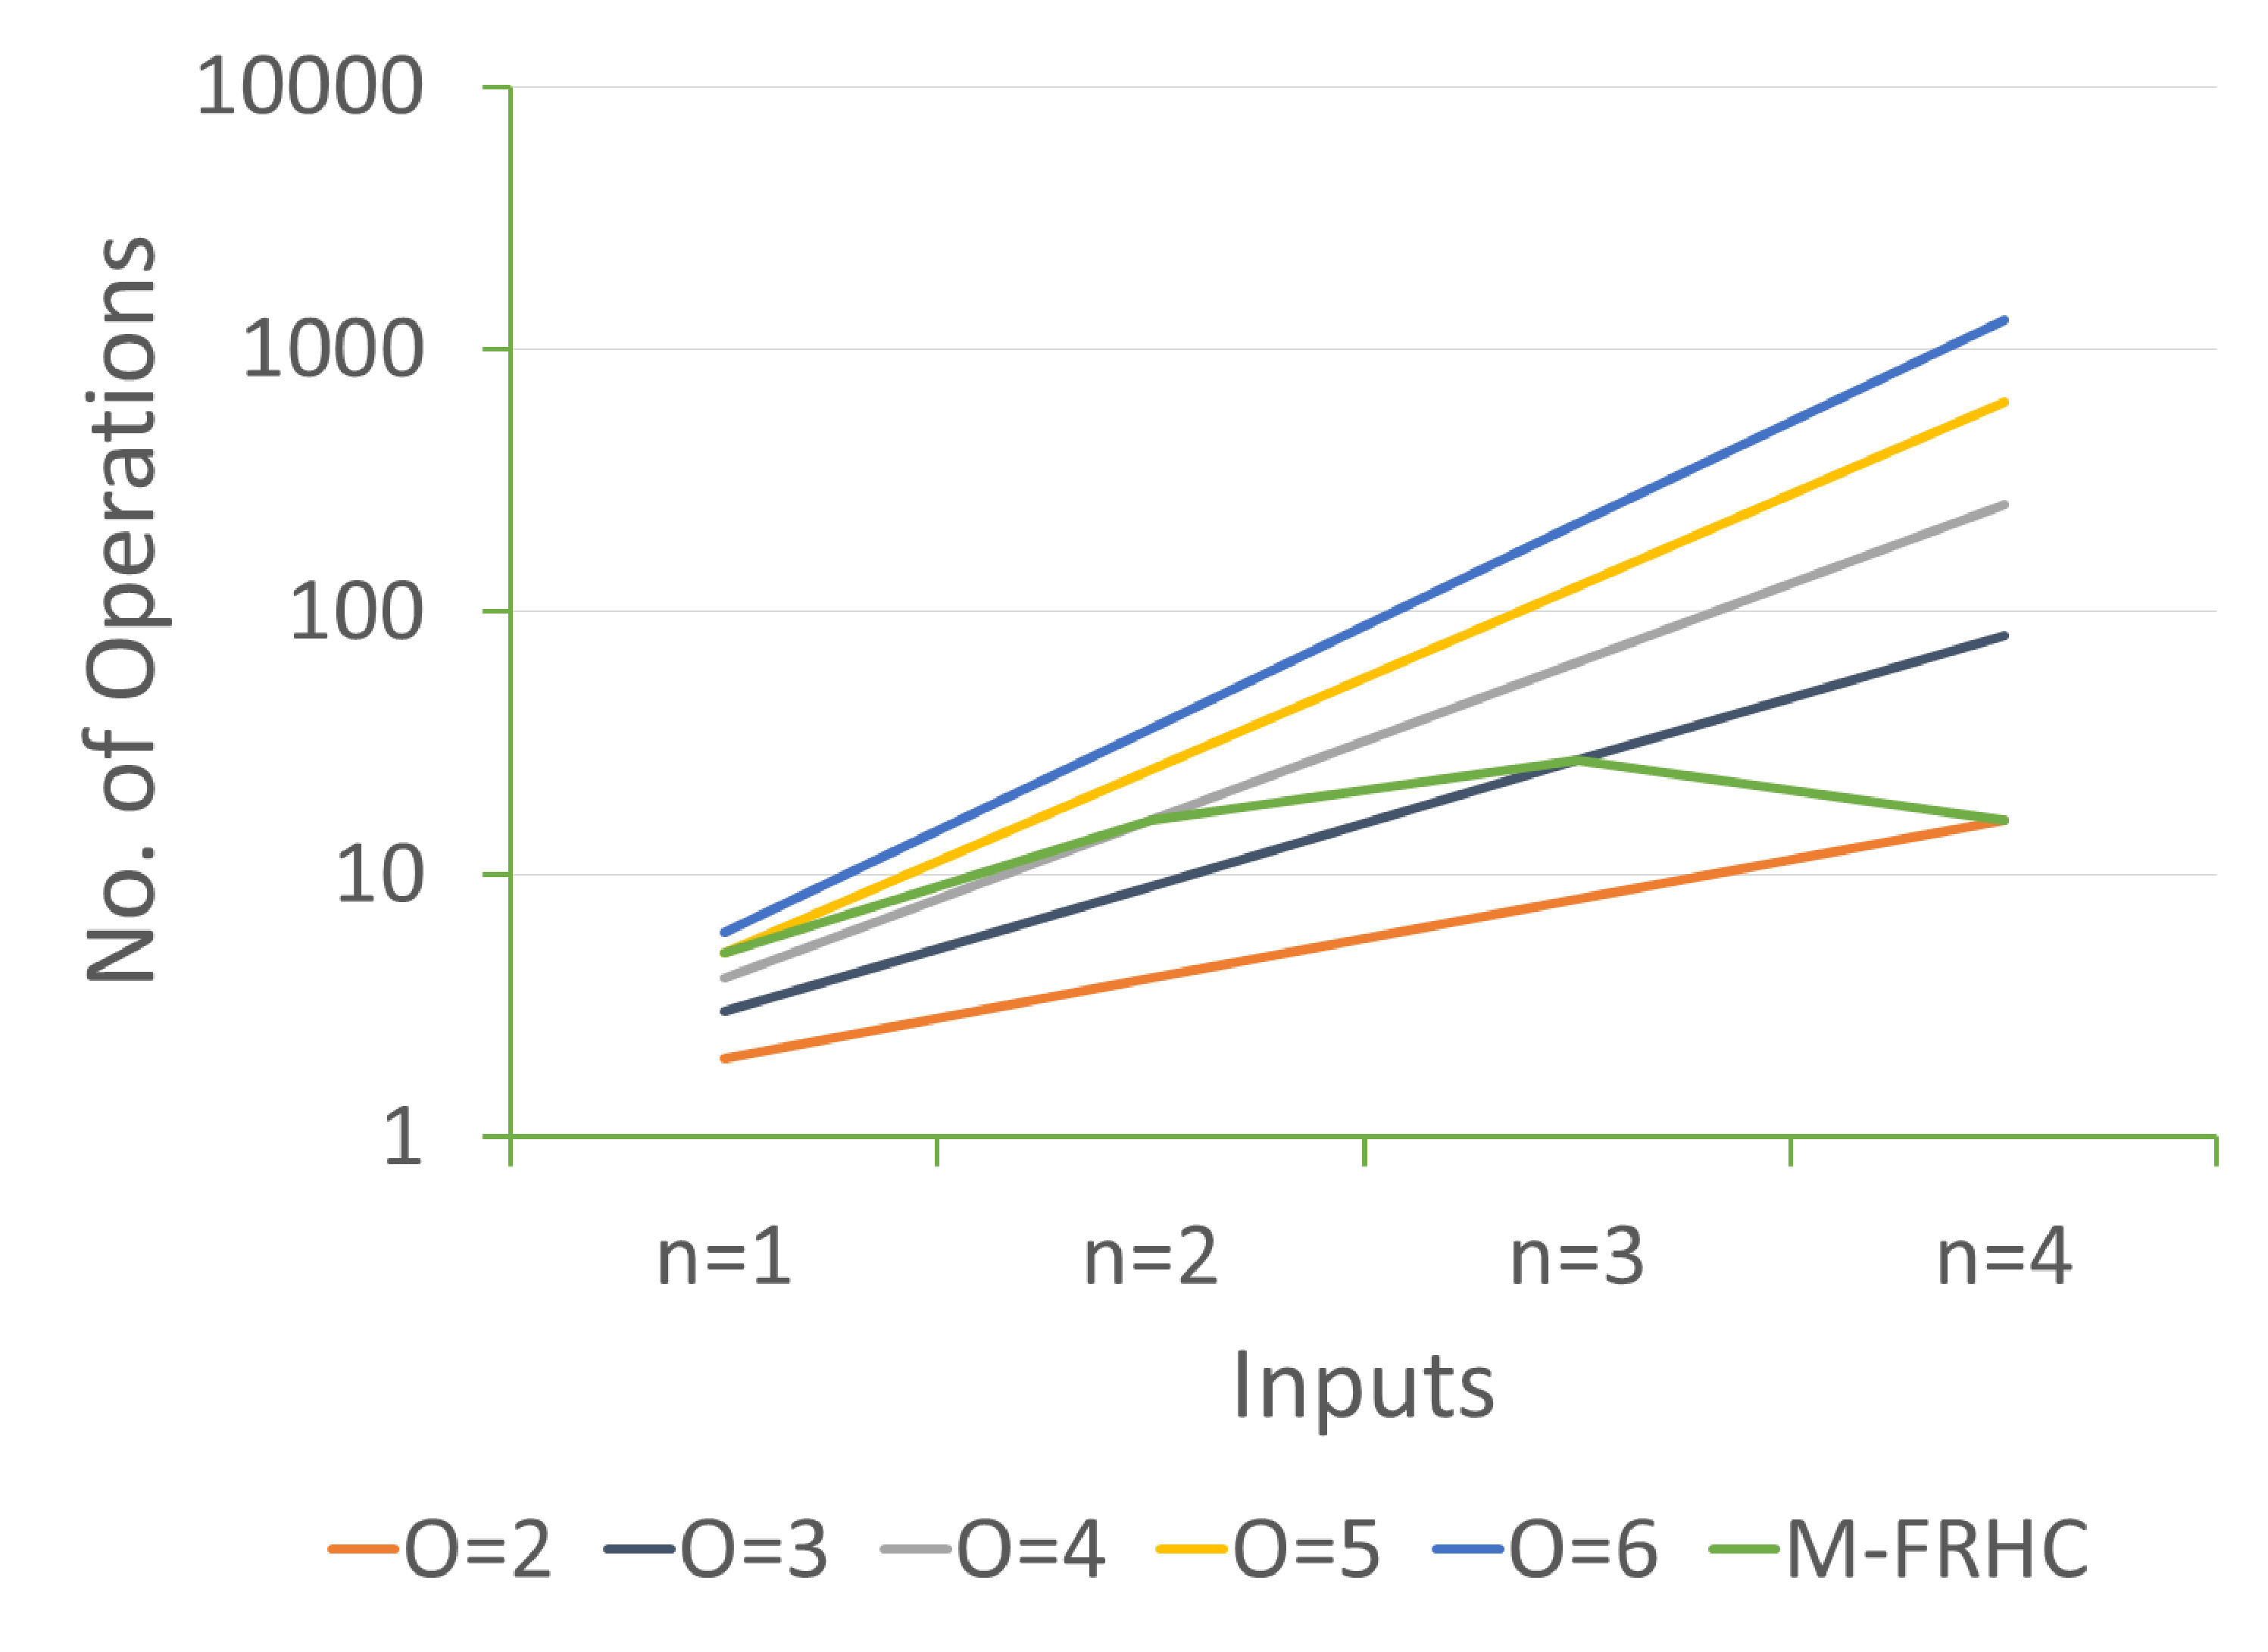
\includegraphics[width=0.95\linewidth]{Chapter2/chapter2/plot_MFRHC}
	\caption{Inputs vs No. of Operations with constant overlaps}
	\label{fig:plot_MFRHC}
\end{figure}

In G\hyp{}FLCS, implementation of M-FRHC will allow the number of overlaps to vary suitable with conjunction to the complexity of the control system. Here, $ n_{op} $ per fuzzy inference becomes a programmable parameter in this proposed M-FRHC rule reduction technique. The effect of this complexity reduction is presented in Figure \ref{fig:plot_MFRHC}. It can be observed that the number of fuzzy inferences or operations varies exponentially against the number of inputs considering a different number of overlapping membership functions except the plot corresponding to M-FRHC. In this G-FLCS implementation, $ \forall n = \left\{ {1,2,3,4} \right\} $, $ O={5,4,3,2} $. Using these values in \eqref{eq:ncells}, in the proposed M-FRHC based G-FLCS design, $ N_{cells} =\left\{ {5,16,27,16} \right\}  $ This causes a slight drop in the green line in Figure 2.2 specially when value of n transits from 3 to 4. It is observed from Figure \ref{fig:plot_MFRHC}, that the plot corresponding to M-FRHC is considerably parallel to x-axis on a logarithmic scale where all others are linearly increasing. This implies that, M-FRHC generates a constant number of operations per inference for all inputs $ N \to [1,4] $ whereas, the complexity of the G-FLCS increases exponentially with the increase in the number of inputs. It also caters a flexibility of adjusting the uncertainties on the boundary between the fuzzy sets. Hereby, \eqref{eq:FRHC_O} can translated to \eqref{eq:FRHC_OM2}.

\begin{table}[h!]
	\centering
	\caption{Computed $n_{op}$ with varying Inputs and Overlaps}
	\begin{tabular}{c|ccccc}
		\hline  
		%				InputOverlap & 2 & 3 & 4 & 5 \\
		\noalign{\vskip 1mm} \diagbox{$N$}{$O_l$} & 2 & 3 & 4 & 5 & 6\\
		\hline \noalign{\vskip 1mm} 
		1 & 2 & 3 & 4 & 5 & 6\\
		2 & 4 & 9 & 16 & 25 & 36\\
		3 & 8 & 27 & 64 & 125 & 216\\
		4 & 16 & 81 & 256 & 625 & 1296\\ \noalign{\vskip 1mm} 
		\hline
	\end{tabular}
	\label{tab:Nops}
\end{table}

\begin{equation} \label{eq:FRHC_OM2}
\begin{array}{l}
{\psi _I} = \left[ {\begin{array}{*{20}{c}}
	{{\mu _1}\left( {{i_1}} \right)}& \cdots &{{\mu _{{o_l}}}\left( {{i_1}} \right)}\\
	\vdots & \ddots & \vdots \\
	{{\mu _1}\left( {{i_N}} \right)}& \cdots &{{\mu _{{o_l}}}\left( {{i_N}} \right)}
	\end{array}} \right]\\~\\
{P_I} = \left[ {\begin{array}{*{20}{c}}
	{{p_1}\left( {{i_1}} \right)}& \cdots &{{p_{{o_l}}}\left( {{i_1}} \right)}\\
	\vdots & \cdots & \vdots \\
	{{p_1}\left( {{i_N}} \right)}& \cdots &{{p_{{o_l}}}\left( {{i_N}} \right)}
	\end{array}} \right]
\end{array}
\end{equation}
where, there are $ O_l $ number of elements in $ \psi _I $. $ O_l $ represents the number of overlaps considered.

It is required to track the index of membership function and link it to the Rulebase matrix appropriately. Hereby, in this scheme it is required to implement the vector combination operation on $ {P_I} $ along with $ {\psi _I} $ to generate $ C_{{R_k}} $ and $ C_{{R_v}} $ respectively. $ {C_{{R_k}}} $ and $ {C_{{R_v}}} $ can be represented as

\[\begin{array}{l}
{C_{{R_k}}} = {\Lambda _c}\left( {{P_1},{P_2}, \ldots {P_N}} \right)\\
{C_{{R_v}}} = {\Lambda _c}\left( {{\psi _1},{\psi _2}, \ldots {\psi _N}} \right)
\end{array}\]
where $ \Lambda _c $ denotes the vector combination as defined in Lemma \ref{lem:VecComb}.

$ C_{{R_k}} $ is required to derive the index of the Rulebase matrix $ R_b $.  The index $ k_x $ of Rulebase matrix $ R_b $ can be derived by
\begin{equation}
{k_x} = \left\{ {\sum\limits_{j = 0}^{N - 1} {{C_{{R_k}}}\left( {x,j} \right),\forall x|x \to \left[ {1,{N^{{O_l}}}} \right]} } \right\}
\end{equation}
\\
\begin{equation} \label{eq:Rb_kx}
\begin{array}{l}
{R_b}\left( {{k_x}} \right) = {c_j}\\
{c_j} \to \left[ {1,M} \right]\forall j = \left\{ {1,2, \ldots {N_R}} \right\}
\end{array}
\end{equation}
\par
Finally, fuzzy output is derived from the following relationship. 
\begin{equation} \label{eq:MFRHC-final}
{\theta _f}({c_j}) = \bigcap\limits_{{k_x} = 0}^{n_{op} - 1} {\left( {{\theta _f}\left( {{R_b}\left( {{k_x}} \right)} \right),\left( {\bigcup\limits_{l = 0}^{N - 1} {\overrightarrow {{C_{{R_v}}}\left( l \right)} } } \right)} \right)} 
\end{equation}
where, $ {\theta _f} $ is  fuzzy output vector, index $ k_x $ varying from $ 0  $ to number of fuzzy operations $ (n_{op} - 1) $, $ R_b $ is the rule base matrix, $ C_{R_V} $ represents the vector combination of non-zero fuzzified input values, $ l $ varying from $ 0 $ to $ N-1 $ and $ \bigcap {} $  and $ \bigcup {} $ representing t-norm and s-norm operations respectively. It is important to analyze the data path of the system architecture to take advantage of the device architecture on which it will be deployed. The target processor is a VLIW based DSP device. The system architecture can be modified at later stage however, there should be scope for data and instruction level parallelism. 

\subsection{Modified and Thresholded Fired Rulebase Hyper Cube (MT-FRHC)}
In this section, MT-FRHC is proposed to tackle the challenges of removing unwanted firing of rules by insignificantly close to zero fuzzy values. The removal of these rules significantly increases computational speed without affecting the output accuracy. This can be achieved by introducing a threshold in \eqref{eq:FRHC_OM2}. Consider an element in $ {\psi _I} $ that assume a very low value and eventually may fire one or more rules. Based on T-Norm operators, weights of all these fired rules are likely to be close to the value of the element. This value will produce a minuscule $ \lambda $ cut-set at the fuzzy output set if there exist no value greater than the current weight assigned to the corresponding member of the fuzzy set. The effect of this $ \lambda $ cut-set is likely to result in a very fine change in output after defuzzification. Thus analytically, it is beneficial to remove these values from  $ {\psi _I} $ based on a suitable threshold.  

Considering all elements of ${\psi _I} $ is greater than threshold $ \tau $, ${\psi _I}^T $ can be computed as 
\begin{align} \label{eq:MTFRHC}
{\psi _I}^T = \{ {d_{jq}}|&({d_{jq}} \in {\psi _I},\forall j \to [1,{O_l}],q \to [1,N]) \\ \nonumber
&\text{ and }{d_{jq}} > \tau \}
\end{align} 
This implies,
\[{d_{jq}} \notin {\psi _I}\forall {d_{jq}} < \tau \]
where, $ {d_{jq}} $ represents individual elements of matrix $ {\psi _I}^T $.
As the elements in $ {\psi _I} $ decreases, the row vectors in $ {C_{{R_v}}} $ and $ {C_{{R_k}}} $ decreases. The number row vectors is equal to $ n_{op}  $ and thus it can be inferred that $ \tau $ is inversely proportional to the computational complexity.

Consider the following example where the rules are 
\[\begin{array}{l}
If~input~I~is~M{F_1}~then~Output~O~is~{P_1}\\
If~input~I~is~M{F_2}~then~Output~O~is~{P_2}\\
If~input~I~is~M{F_3}~then~Output~O~is~{P_3}
\end{array}\]
and the input space is fuzzy partitioned as in Figure \ref{fig:MTFRHC_plot_2}.
\begin{figure}[h]
\centering
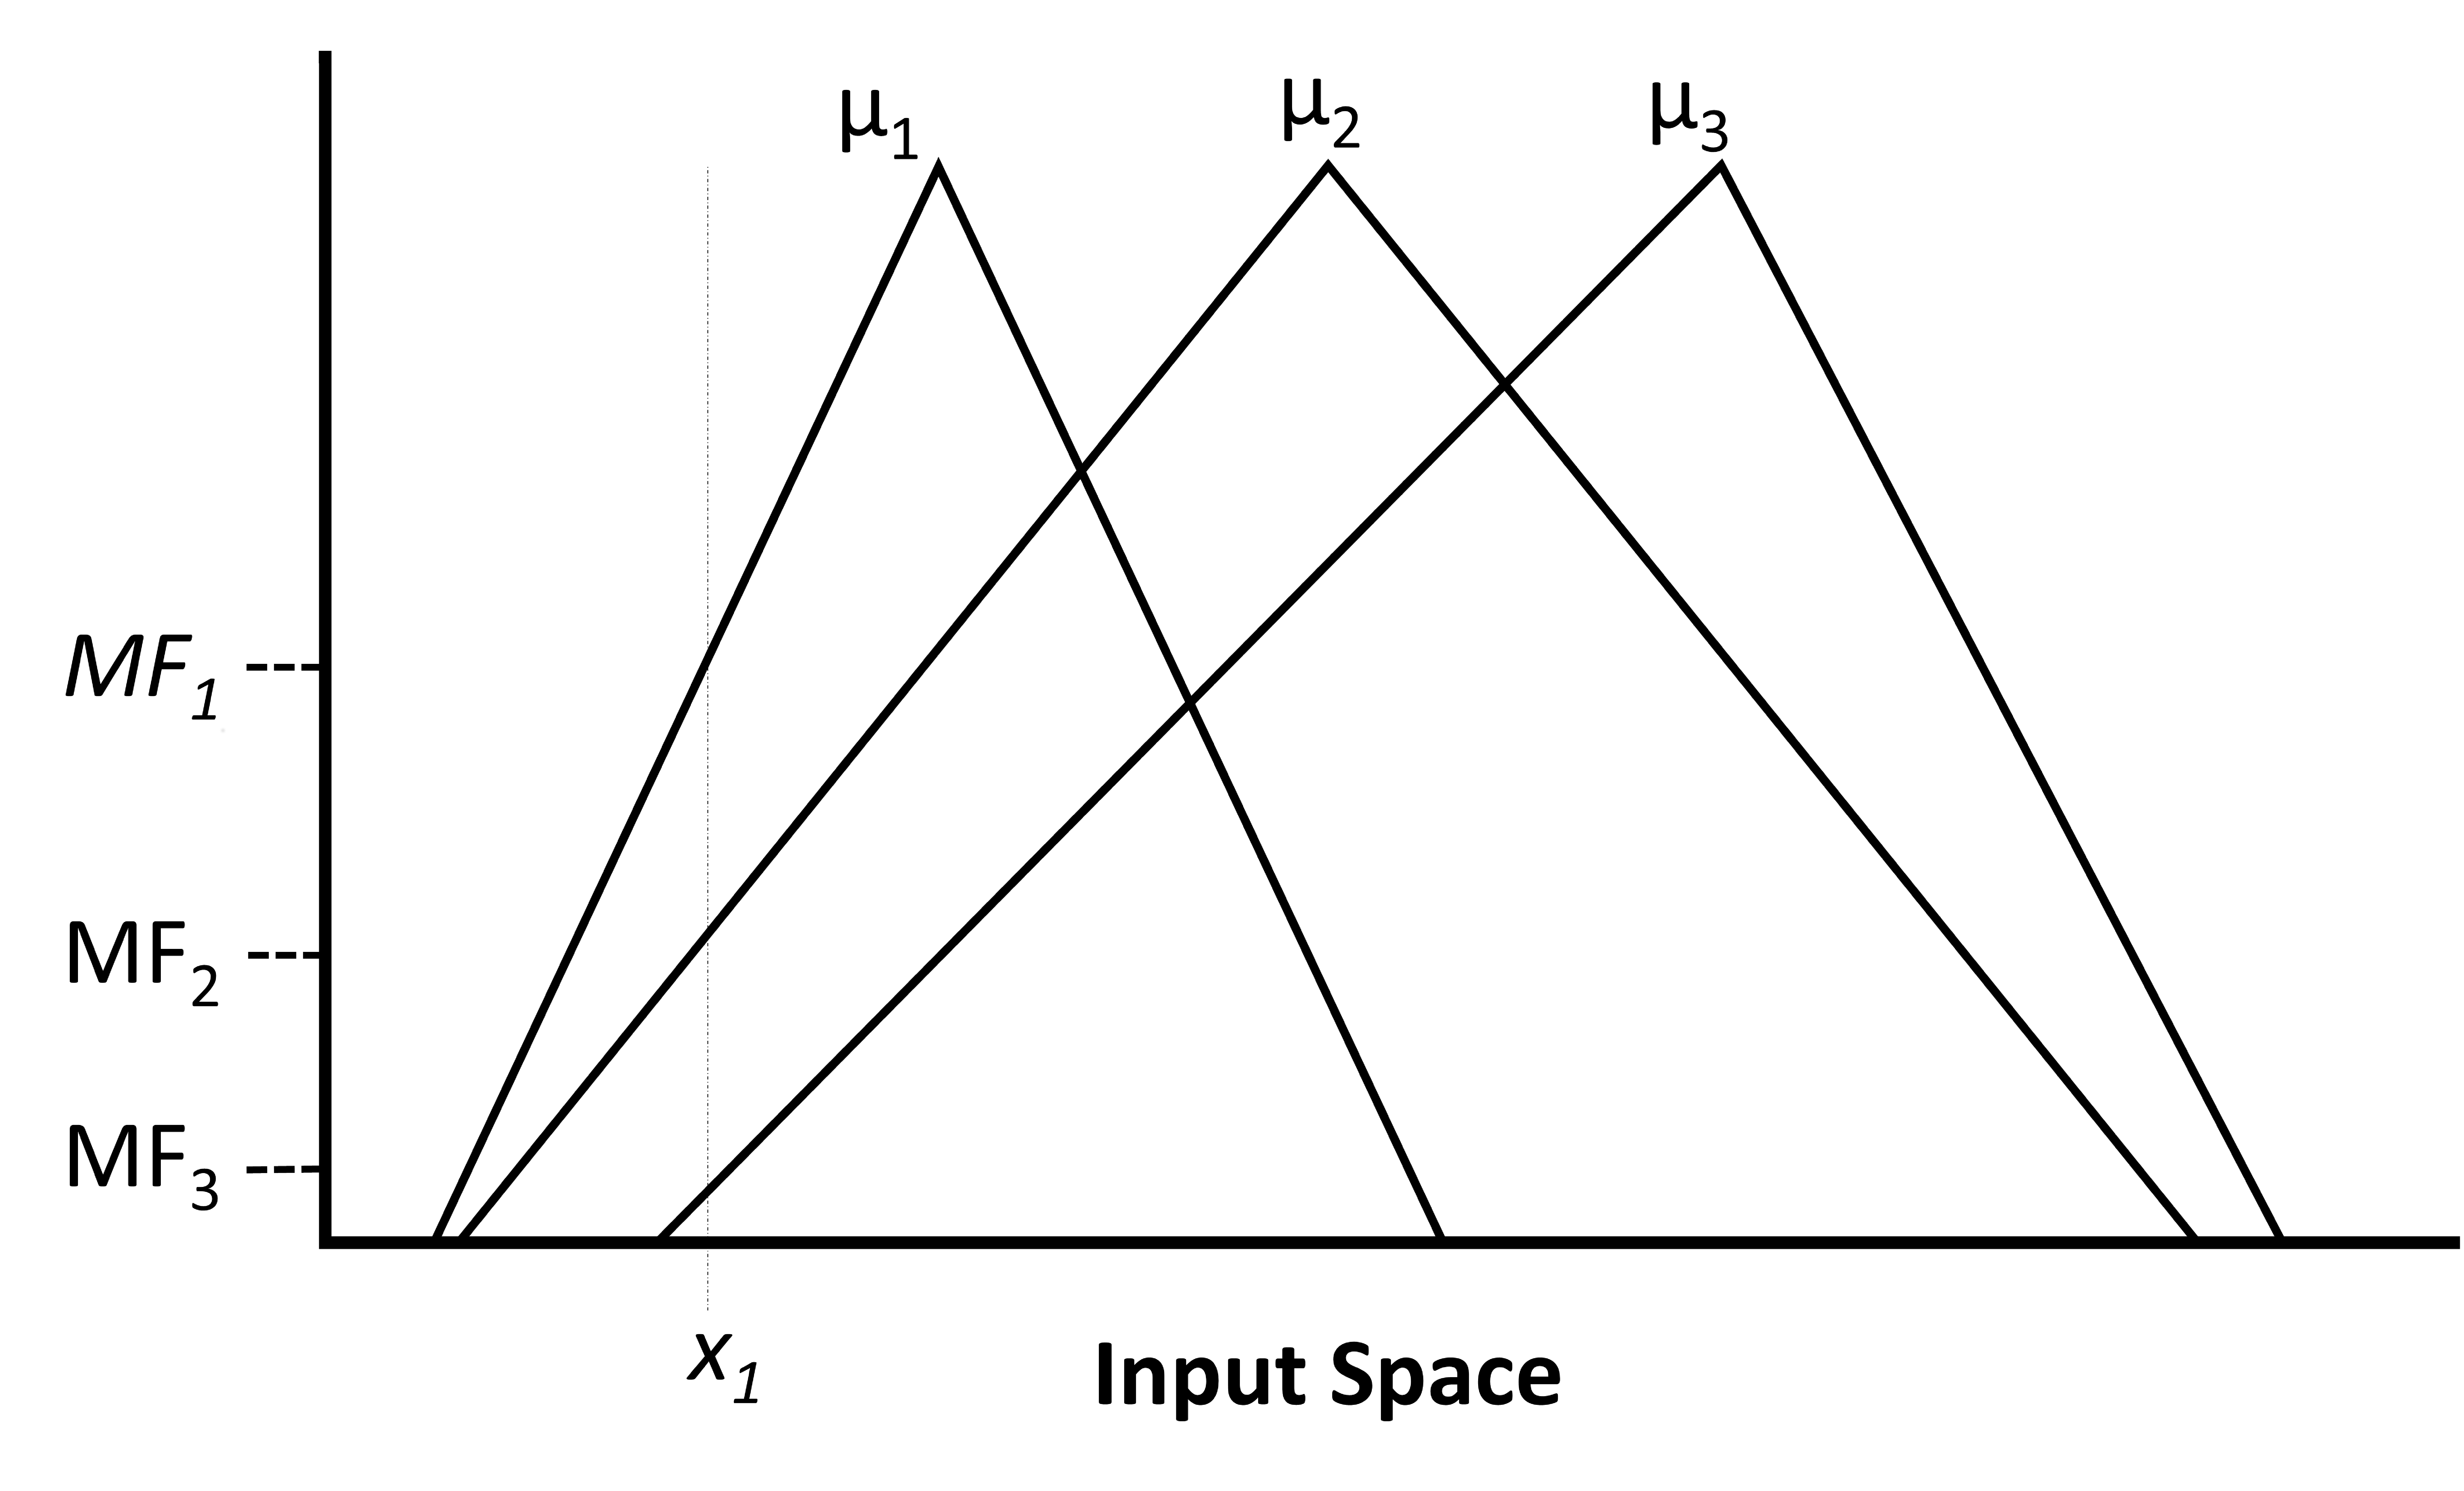
\includegraphics[width=0.7\linewidth]{Chapter2/chapter2/MTFRHC_plot_2}
\caption{An Example: Input Membership Function}
\label{fig:MTFRHC_plot_2}
\end{figure}

Assuming, $N_Cells=5$ with one input and the input value being $x_1$, the M-FRHC output is,
\[\left [M{F_1},~M{F_2},~M{F_3}\right ]\]
It is obvious from  Figure \ref{fig:MTFRHC_plot_2} that, $ M{F_1}>M{F_2}>M{F_3} $. Now if $M{F_3}$ is very very small, then its effect on the output is small. However, due to its firing, an additional rule is active and it gets evaluated. This evaluated rule is extremely weak as the weight it carries (from $M{F_3}$) is very small. Thus, if this rule is excluded from the computation, the accuracy of the system does not change much, but the reduction in computation is reduced by one-third(instead of 3 rules, only 2 rules are evaluated) in above example. Thus in MT-FRHC, a threshold $\tau $ is expended to discard rules which carry extremely small weight.


\section{Defuzzification}
\begin{figure}[b!]
\centering
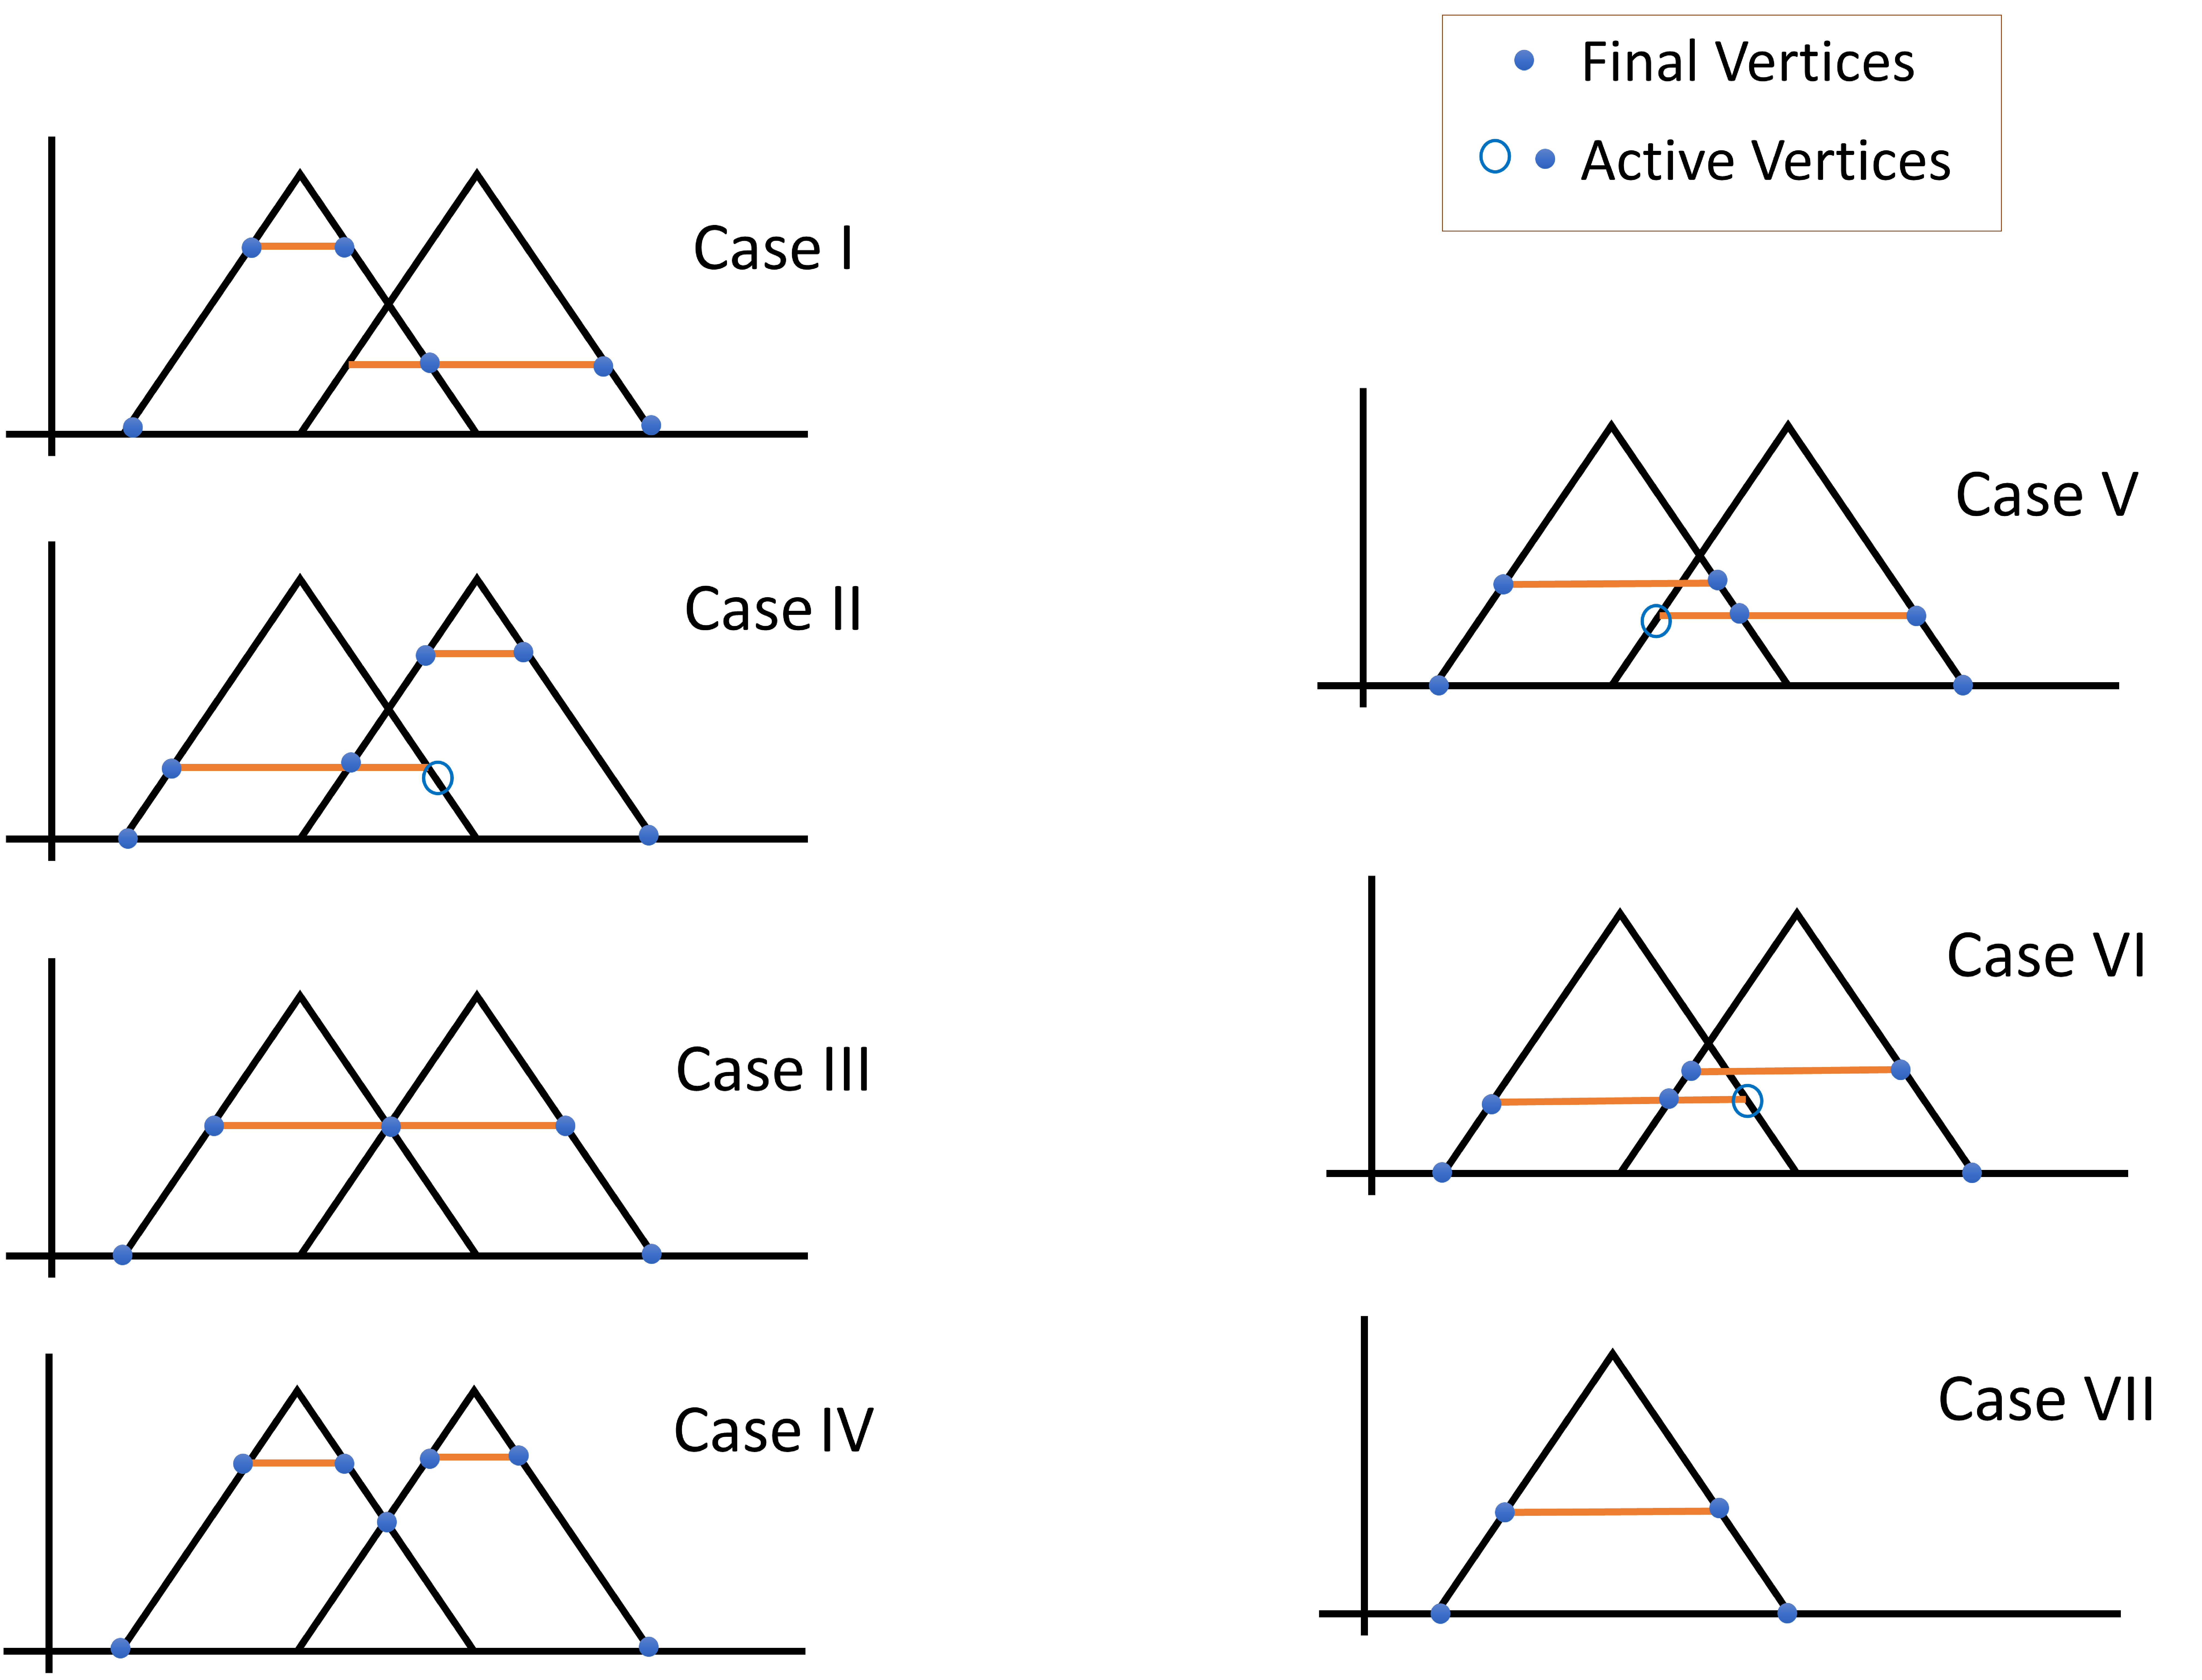
\includegraphics[width=1\textwidth,,height=15cm]{Chapter2/chapter2/Vertices_cases}
\caption{Various cases for vertices computation for Centroid of Area (COA) Defuzzification}
\label{fig:Vertices_cases}
\end{figure}

As discussed in the earlier section, to generate a quantifiable output using fuzzy logic that can be implied in a real system, defuzzification process is obligatory. Inference engine in a FLCS will have a number of rules that transform variables into a fuzzy result described in terms of membership in fuzzy sets. The defuzzification process converts output expressed in fuzzy sets to crisp output using MFs. It employs certain mathematical operations to interpret the membership degrees of the fuzzy sets into a particular decision or real value. There are number of defuzzification algorithms in literature \cite{Saletic2006,Ross2010,Lee1990,Lee1990a}. The varied processes of defuzzification yields different crisp output. The most widely used defuzzification methods are discussed further.

\subsection{Defuzzification Algorithms}
Leekwijck et. al. \cite{Leekwijck1999} classified defuzzification methods broadly in to 
\begin{enumerate}
	\item Maxima methods and its derivatives,
	\item Distribution methods and its derivatives,
	\item Area methods, and
	\item Miscellaneous methods.
\end{enumerate}
Leekwijck et. al. claim that the \textit{Maxima} methods are suitable candidates for fuzzy reasoning systems whereas the \textit{Area} methods display the attribute of continuity that makes them appropriate for FLCs. Zavala et. al.\cite{Zavala2011} states that among numerous different defuzzification methods available in literature, most used for hardware purposes are Center of Area (CoA) which is classified under Area methods and Mean Of Maxima which is classified under Maxima methods. WA defuzzification method is the also among most frequently used defuzzification technique which is classified under Area methods. Therefore, since our target applications are fuzzy control, CoA and weighted average (WA) is ultimately chosen as the defuzzification method for proposed hardware G\hyp{}FLCS. 

\subsubsection{Weighted Average Defuzzification Technique}
WA defuzzification method is the most frequently used defuzzification technique for fuzzy controllers owing to its low computational complexity. It can even be easily implemented on slow processors like microcontrollers for real-time applications. But this technique can be applied to symmetrical output MFs. The WA method is computed by weighting each output MF by its respected maximum MF value and accumulating them. This can be represented as,
\[{X_{WA}} = \frac{{\sum {{\mu _{\widetilde C}}\left( {\overline x } \right) \cdot \overline x } }}{{\sum {{\mu _{\widetilde C}}\left( {\overline x } \right)} }}\]
where $ \overline x $ represents centroid of each symmetric output MF $ {\widetilde C} $. It is generally not used for G-FLCS with asymmetric output MFs \cite{Ross2010}. Although there are many instances where this method is used for FLCs with asymmetric output MFs \cite{Sugeno1985}.

\subsubsection{CoA Defuzzification Technique}
CoA method is commonly known as center of gravity (CoG) defuzzification. It was developed by Sugeno in 1985\cite{Sugeno1985}. CoA is most commonly used technique in fuzzy control and provides good accuracy \cite{Ross2010,Patel2002}. 
Mathematically this technique is represented as
\[{X_{CoA}} = \frac{{\int {{\mu _c}(x)xdx} }}{{\int {{\mu _c}(x)dz} }}\]
where $ {\mu _c}(x)  $ represents membership degree of each output MF.
Continuity and computational efficiency are of utmost importance for hardware G\hyp{}FLCS. In most realization of CoA, calculating the whole area and determining where its weighted midpoint is essential. As it uses all elements from input universe, it requires $ k = {2^n} - 1 $ iterations according to number of bits ($ n $) used for input universe. These techniques aim at reducing resource consumption and computational time without loss of accuracy. 
Some hardware implementation for CoA uses Center of Slice Area Average (COSAA)defuzzification technique proposed by Zavala et. al. \cite{Zavala2011,HernandezZavala2013,Zavala2010}. COSAA uses the summation of midpoints for all $ \alpha - $ levels instead of integrating the area under a curve. 

\subsection{Vertices based Center of Area (VBCoA) Computation}
The existing techniques for defuzzification using CoA have been seen to be computationally time-consuming. One of the most widely used technique is the Riemann sum based CoA computation. Riemann integral is used for deriving the centroid of area in actual method \cite{Patel2002,Leekwijck1999}. Centroid of a polygon can also be computed using their vertices and has been widely used in geospatial applications \cite{Stankute2010}. This feature is used in the proposed VBCoA defuzzification method. To reduce the defuzzification time, a new vertices based CoA (VBCoA) computation method is proposed. The proposed method can be implemented in following steps.
\begin{description}
	\item[Step 1] Generate cut set matrix from all cut points with non-zero fuzzy output values.
	\item[Step 2] Use cut set to segregate into any one of cases as presented in Figure \ref{fig:Vertices_cases}.
	\item[Step 3] Generate intersecting matrix. Intersecting matrix includes intersecting points of output MF.
	\item[Step 4] Generate individual set of vertices from intersecting matrix and cut set matrix for various case structures as in Figure \ref{fig:Vertices_cases}.
	\item[Step 5] Centroid on X-axis can be calculated as 
	\[\begin{array}{l}
	COA = \frac{1}{{6A}}\sum\limits_{i = 0}^{n - 1} {\left( {{y_i} + {y_{i + 1}}} \right)} \left( {{x_i}{y_{i + 1}} - {x_{i + 1}}{y_i}} \right)\\
	A = \frac{1}{2}\sum\limits_{i = 0}^{n - 1} {\left( {{x_i}{y_{i + 1}} - {x_{i + 1}}{y_i}} \right)} 
	\end{array}\]
	where $n\rightarrow $number of vertices, $ x_i\rightarrow $ $ x $ co-ordinate of $ i^{th} $ vertex, $ y_i\rightarrow $ $ y $ co-ordinate of $ i^{th} $ vertex
\end{description}

The steps 1 through 5 can be used to defuzzify fuzzy output $\theta _f$ using COA process in a fast and efficient manner\footnote{Download Code Here: https://goo.gl/83bVna}. The proposed VBCoA defuzzification algorithm and the traditional Riemann sum based defuzzification algorithm were implemented on a C6748 DSP processor with 300 MHz operating frequency. To analyze the efficacy of the proposed algorithm, computation time using the VBCoA were compared to existing Riemann sum based CoA computation technique. A random set of fuzzy output was generated and defuzzified using these two methods. The process was repeated for five times and he observed cycle time is tabulated in Table \ref{tab:centComp}. The randomly generated fuzzy output set appears in the first row of the table. The next two rows shows the consumed cycles and the cycle time (in $\mu$s) respectively for traditional Riemann sum based CoA computation. The final two rows shows the consumed cycles and the cycle time (in $\mu$s) respectively for the proposed VBCoA computation. Table \ref{tab:centComp} reflects that the proposed VBCoA technique provides a slightly better performance in terms of computational time. VBCoA shows approximately 30\% improvement in the cycle time.

 \begin{table}[h]
 	\centering
 	\caption{Centroid computation on C6748 DSP Hardware}
 	\label{tab:centComp}
% 	\resizebox{1\textwidth}{!}{%
 		\begin{tabular}{c|cc|cc}
 			\hline \noalign{\vskip 1mm}
 			\multirow{2}{*}{} & \multicolumn{2}{c|}{Riemann sum} & \multicolumn{2}{c|}{\textbf{VBCoA} Method} \\ \cline{2-5} \noalign{\vskip 1mm}
 			& Cycles & Time($\mu$s) & Cycles & Time($\mu$s) \\ \hline \noalign{\vskip 1mm}
 			{[}0.2,0.5,0.3{]} & 7662 & 25.54 & 5316 & 17.72 \\  \noalign{\vskip 1mm} 
 			{[}0.4,0.3,0.1{]} & 7681 & 25.60 & 5320 & 17.73 \\  \noalign{\vskip 1mm} 
 			{[}0.8,0.8,0.6{]} & 7528 & 25.54 & 5305 & 17.68 \\  \noalign{\vskip 1mm} 
 			{[}0.1,0.7,0.1{]} & 7650 & 25.50 & 5316 & 17.72 \\  \noalign{\vskip 1mm} 
 			{[}0.3,0.2,0.9{]} & 7677 & 25.59 & 5309 & 17.70 \\  \noalign{\vskip 1mm} \hline
 		\end{tabular}
% 	}
 \end{table}
		

\section{Performance Analysis}

%scale=0.1
\begin{figure}[htbp]
	\centering
	\subfloat[Fuzzy PI Approximation FIS: MT-FRHC]{\label{fig:SPlot_MT-FRHC}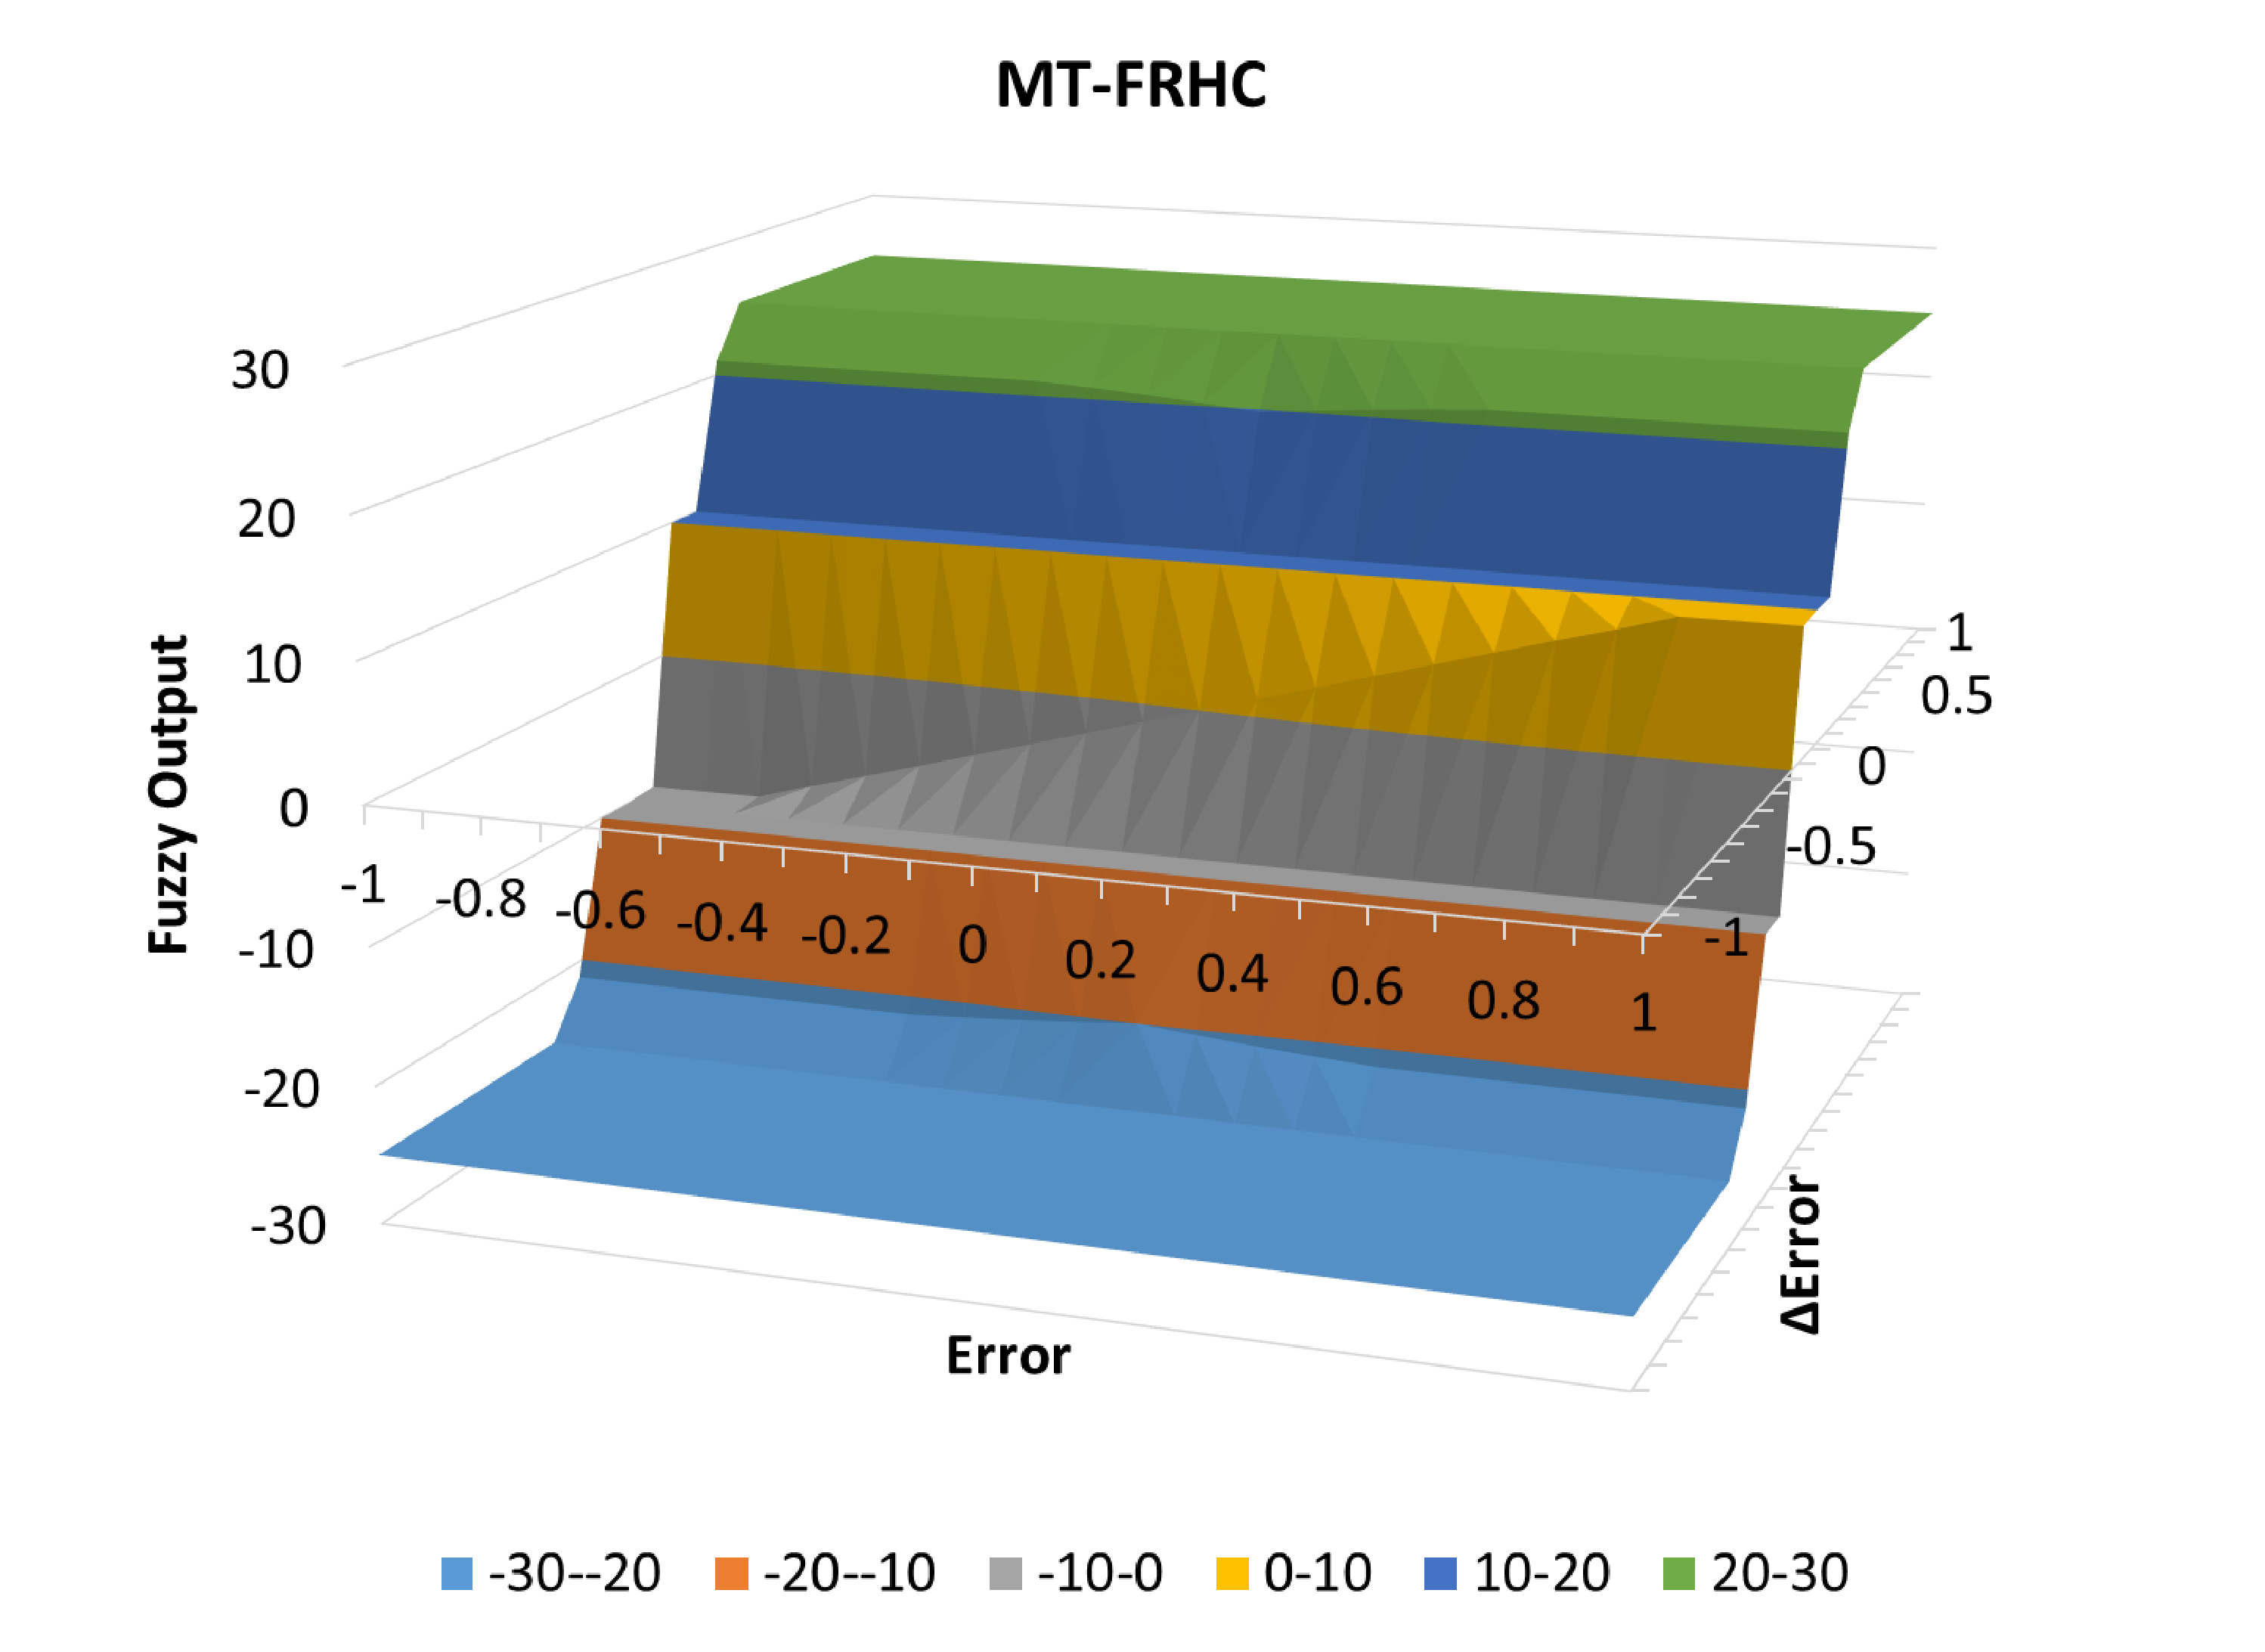
\includegraphics[width=0.6\linewidth]{Chapter2/chapter2/MTFRHC_plot.eps}} \\
	\subfloat[Fuzzy PI Approximation FIS: Matlab Fuzzy Toolbox]{\label{fig:SPlot_MFT}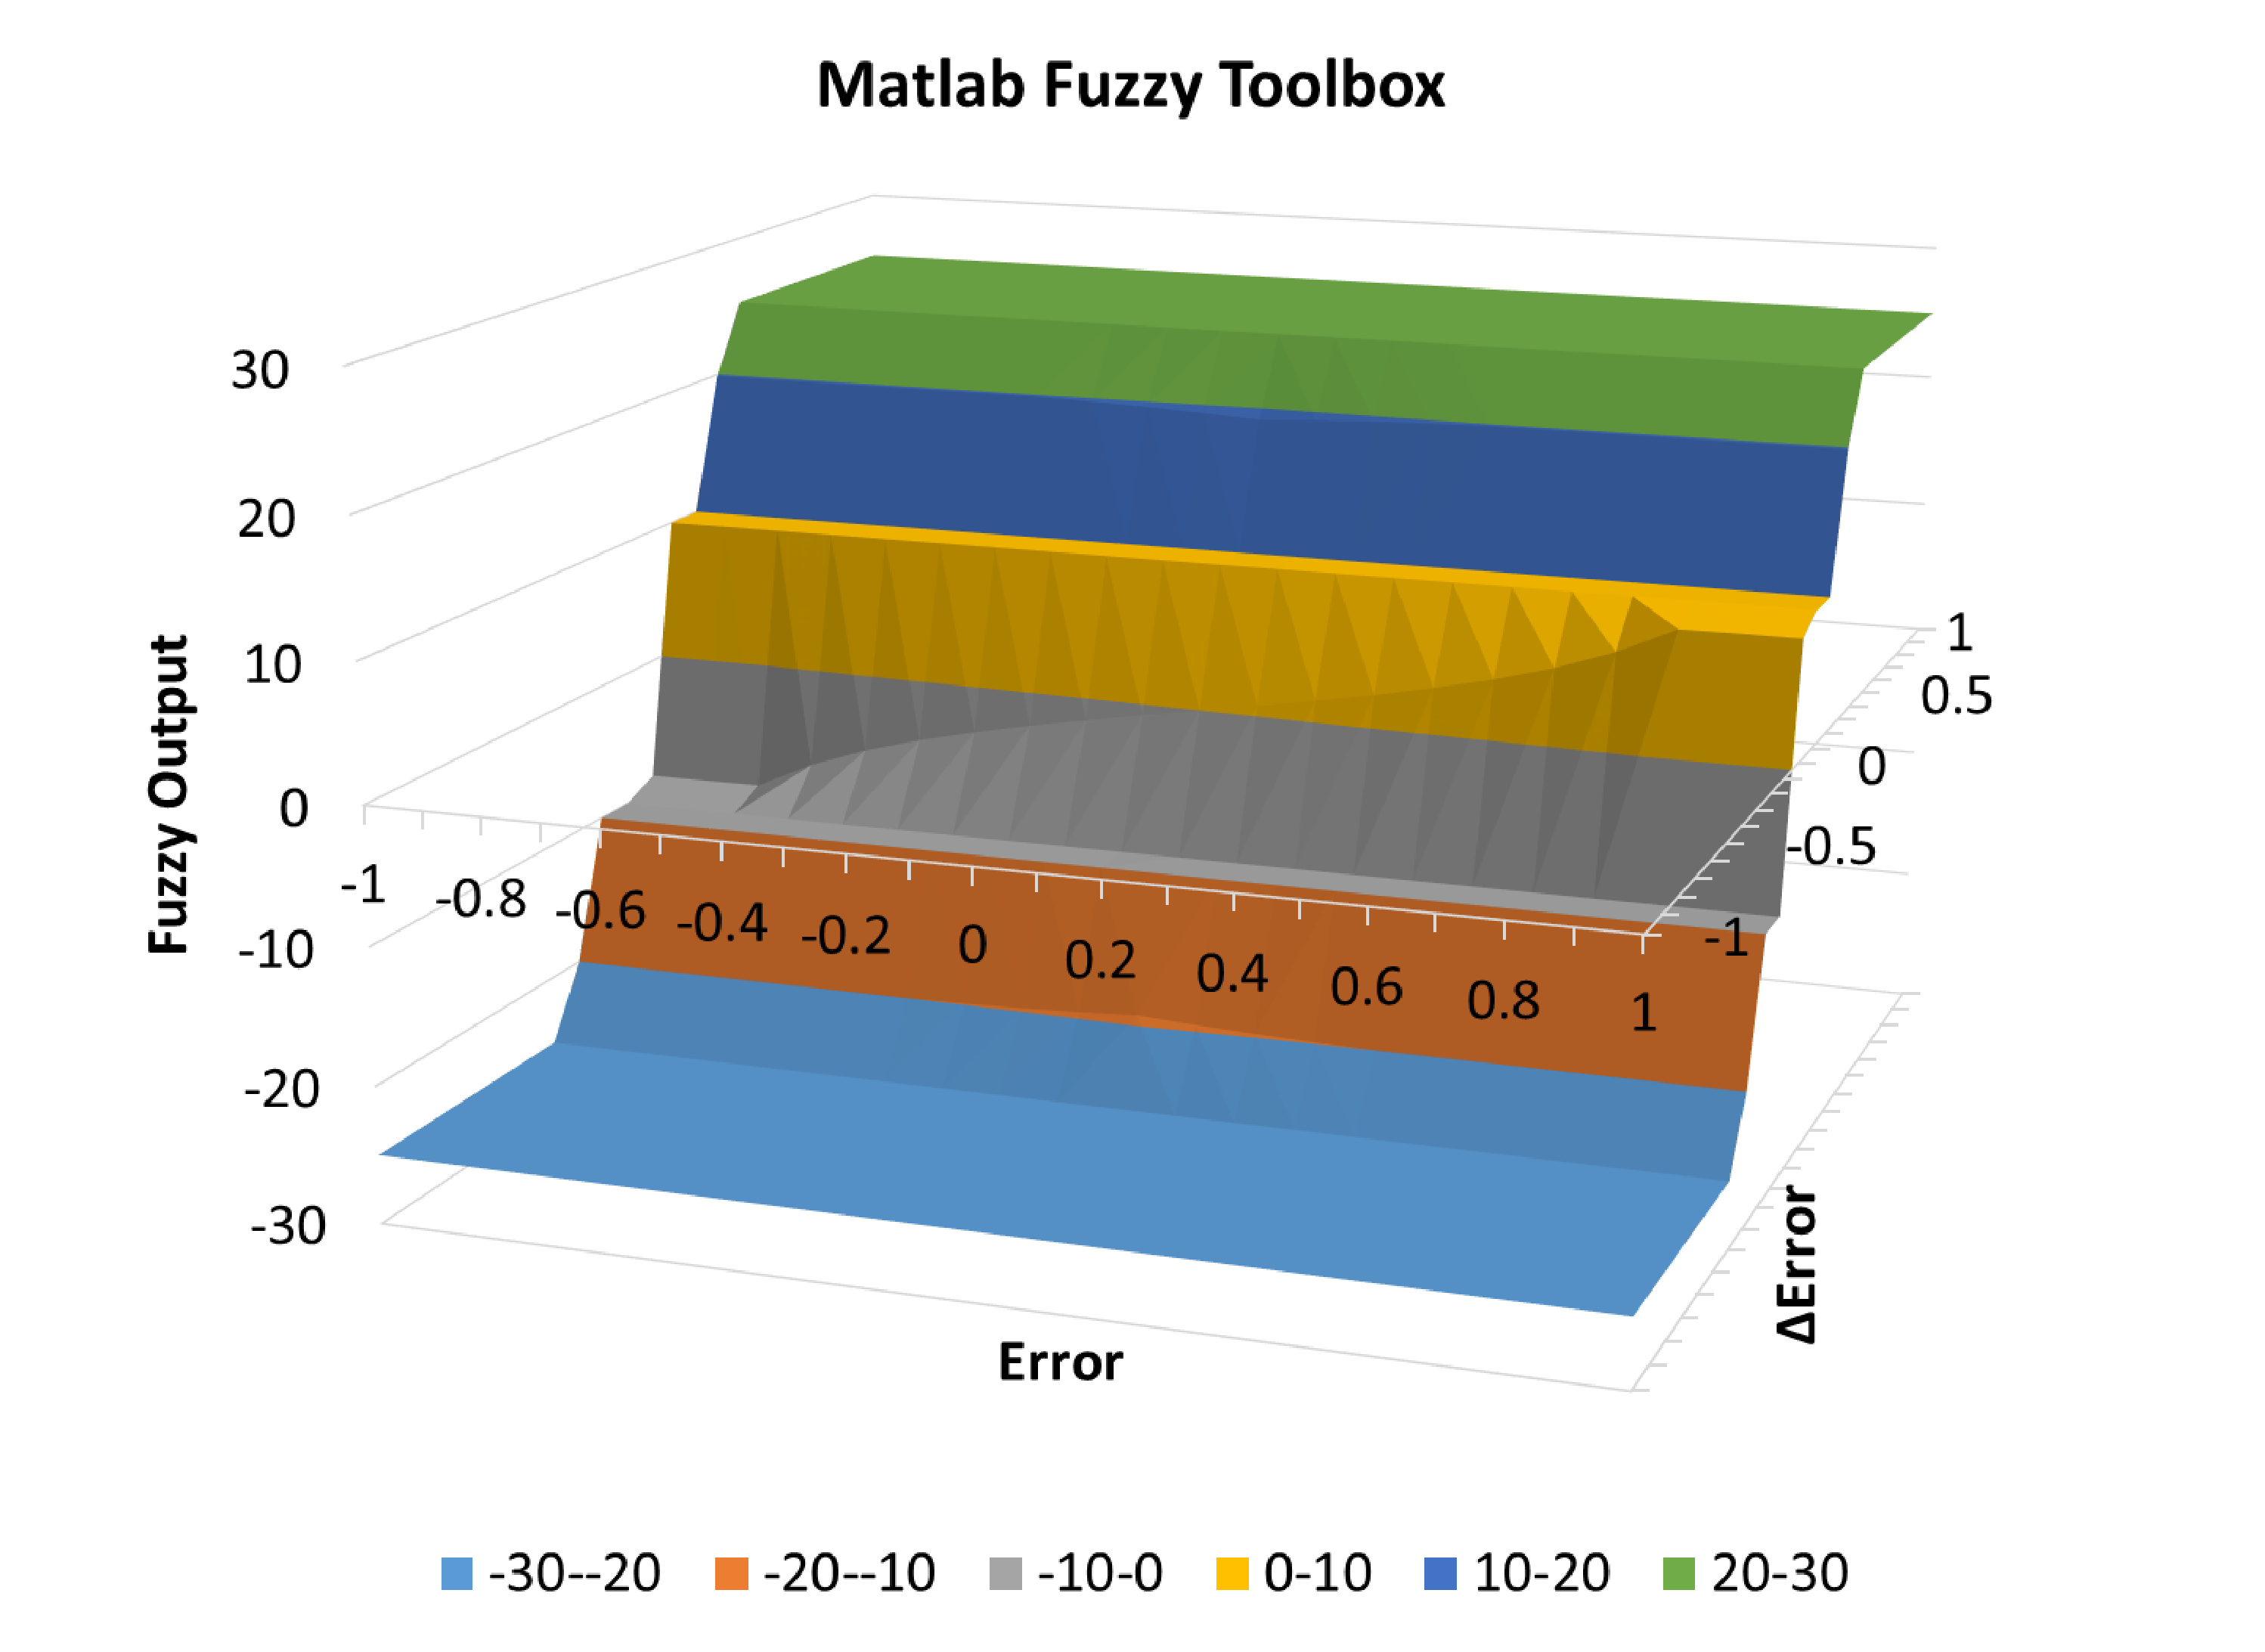
\includegraphics[width=0.6\linewidth]{Chapter2/chapter2/MatlabToolbox_plot.eps}} \\
	\subfloat[Fuzzy PI Approximation FIS: Error Plot]{\label{fig:SPlot_Error}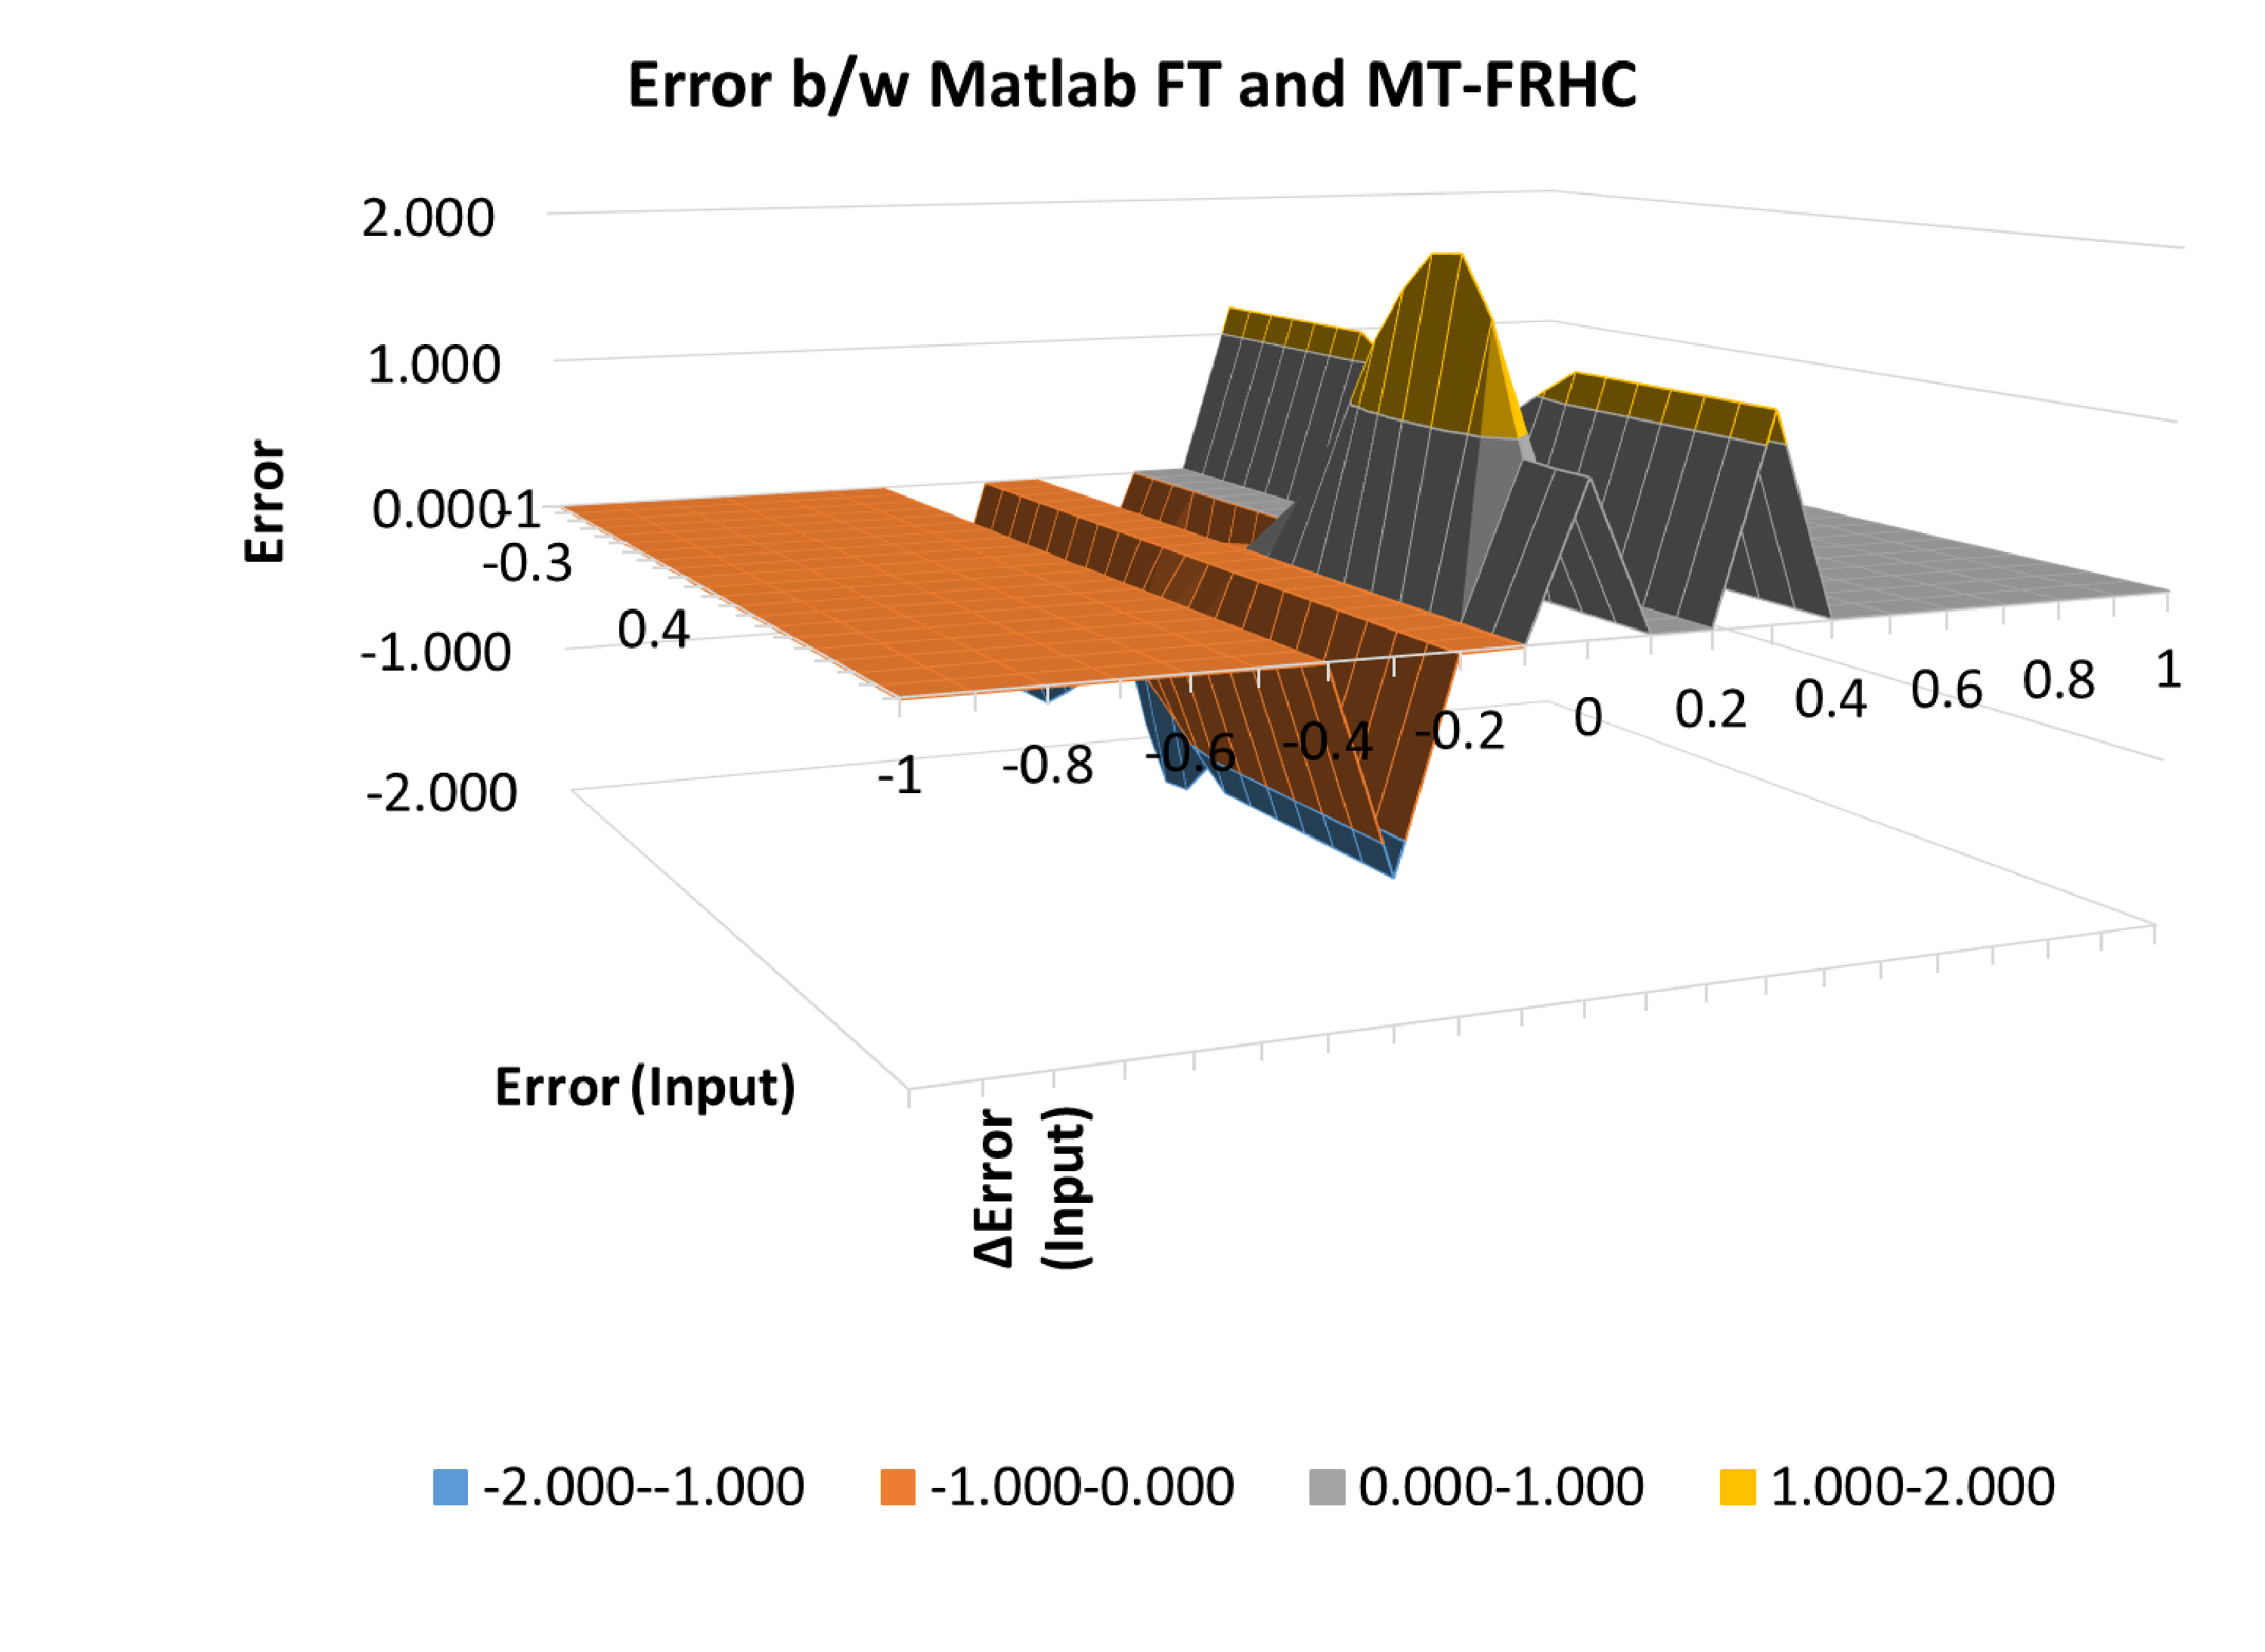
\includegraphics[width=0.6\linewidth]{Chapter2/chapter2/error_plot.eps}}
	\caption{Surface Plot to test Fuzzy Inference Parameter for Fuzzy Inference Structure (FIS) used in Fuzzy PI approximation controller for ACDC motor control \cite{malla2012}}
	\label{fig:SurfacePlot_ACDC}
\end{figure}

\begin{figure}[htbp]
	\centering
	\subfloat[Two Tank FIS: MT-FRHC]{\label{fig:SPlot_MT-FRHC_tank}\includegraphics[width=0.6\linewidth]{Chapter2/chapter2/tank_MTFRHC.eps}} \\
	\subfloat[Two Tank FIS: Matlab Fuzzy Toolbox]{\label{fig:SPlot_MFT_tank}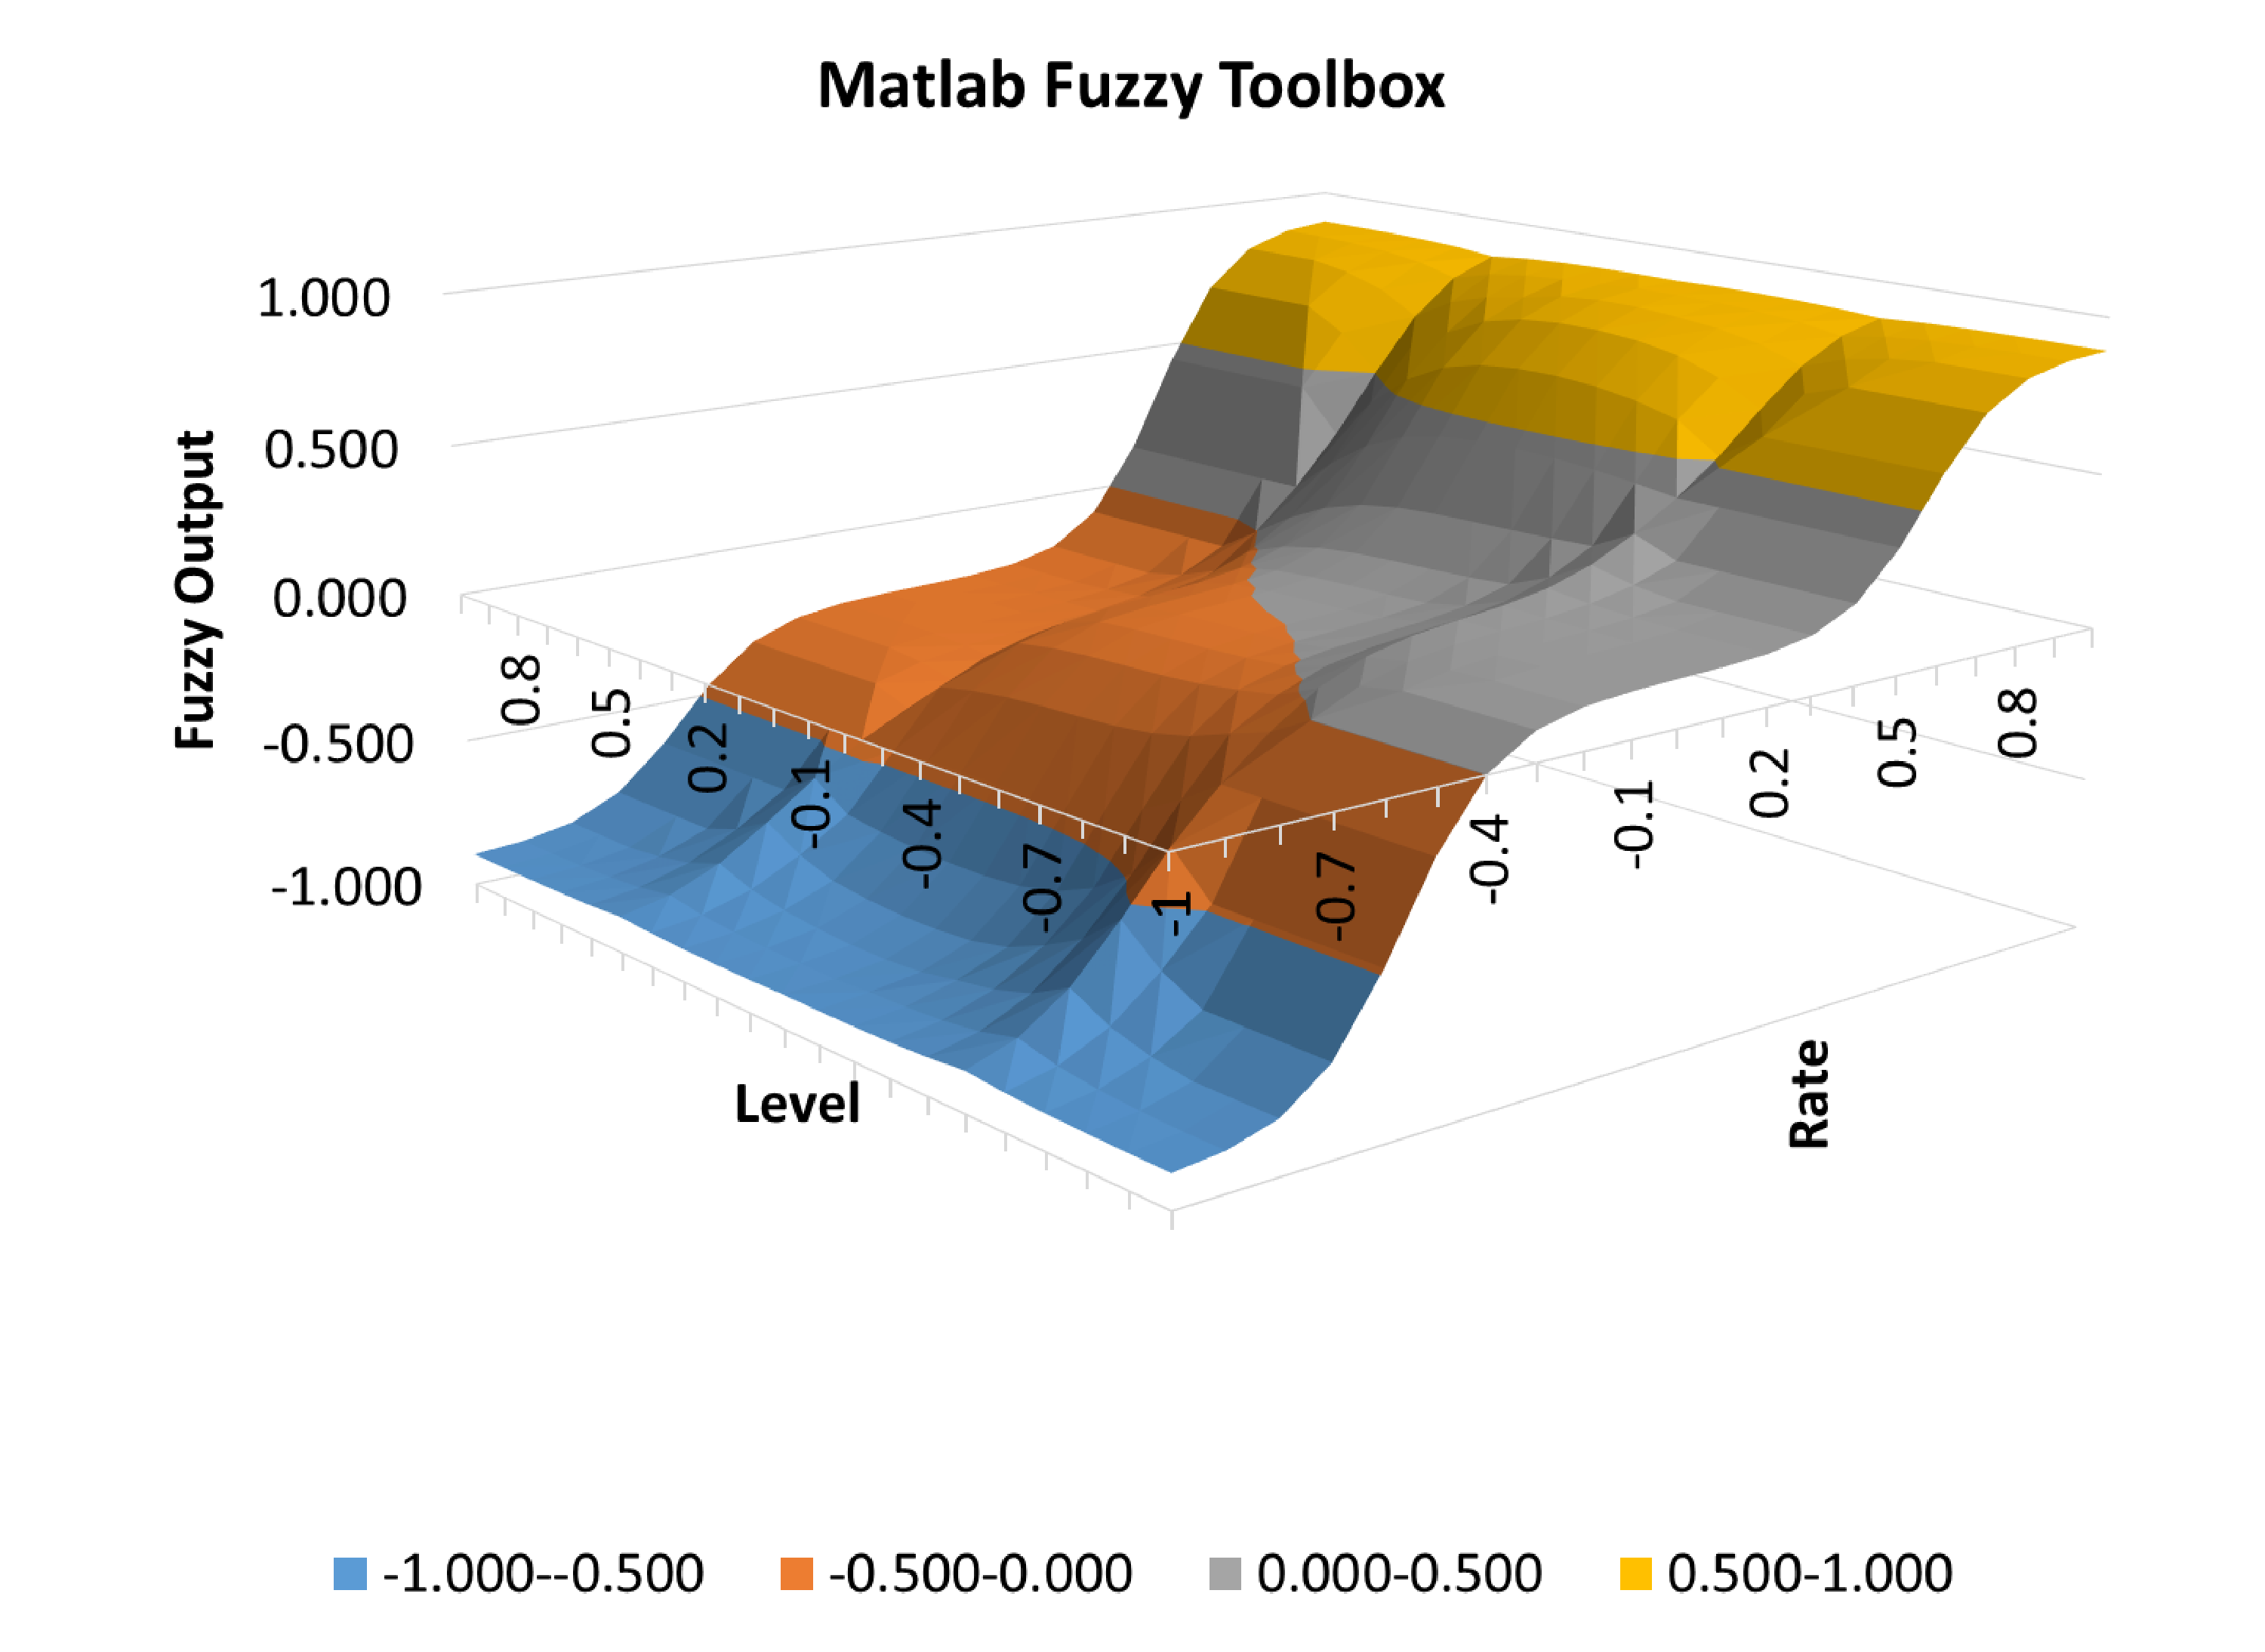
\includegraphics[width=0.6\linewidth]{Chapter2/chapter2/tank_MFT.eps}} \\
	\subfloat[Two Tank FIS: Error Plot]{\label{fig:SPlot_Error_tank}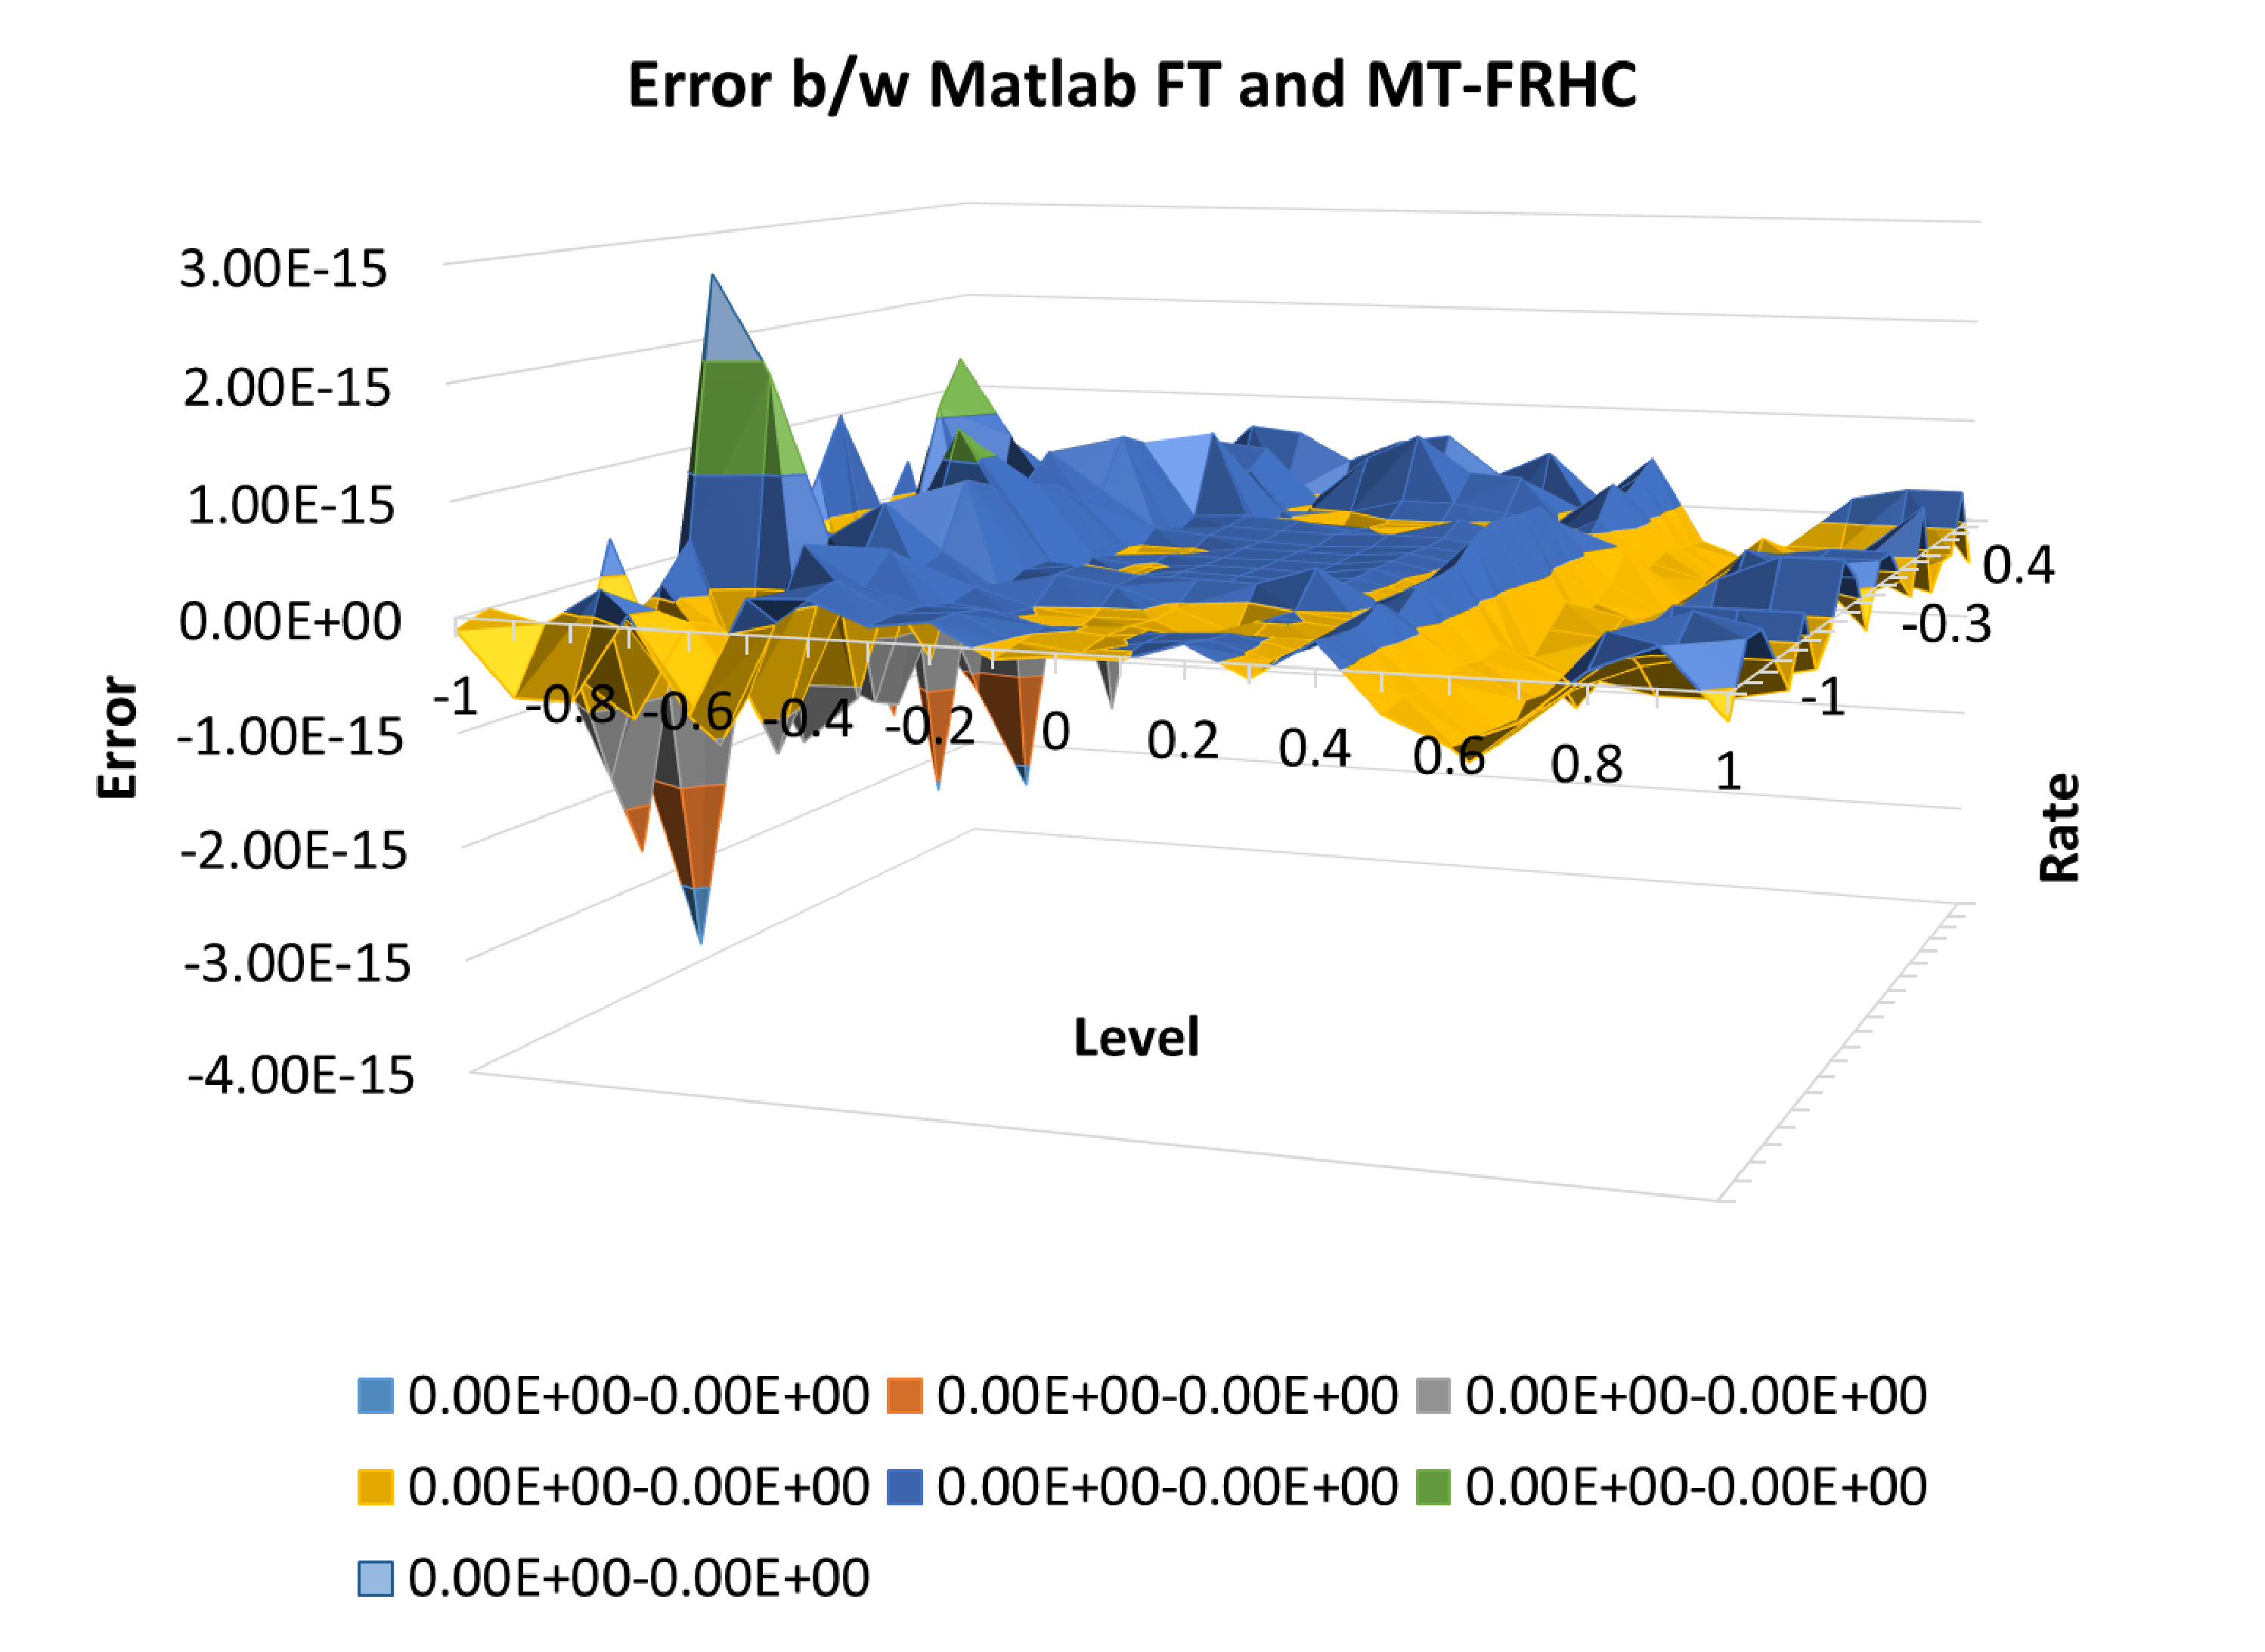
\includegraphics[width=0.6\linewidth]{Chapter2/chapter2/tank_Error.eps}}
	\caption{Surface Plot to test Fuzzy Inference Parameter for Fuzzy Inference Structure (FIS) used in Fuzzy PI approximation controller for Two Tank System \cite{twotank2012}}
	\label{fig:SurfacePlot_tank}
\end{figure}

\begin{figure}[htbp] 
	\centering
	\subfloat[Truck Backer FIS: MT-FRHC]{\label{fig:SPlot_MT-FRHC_truck}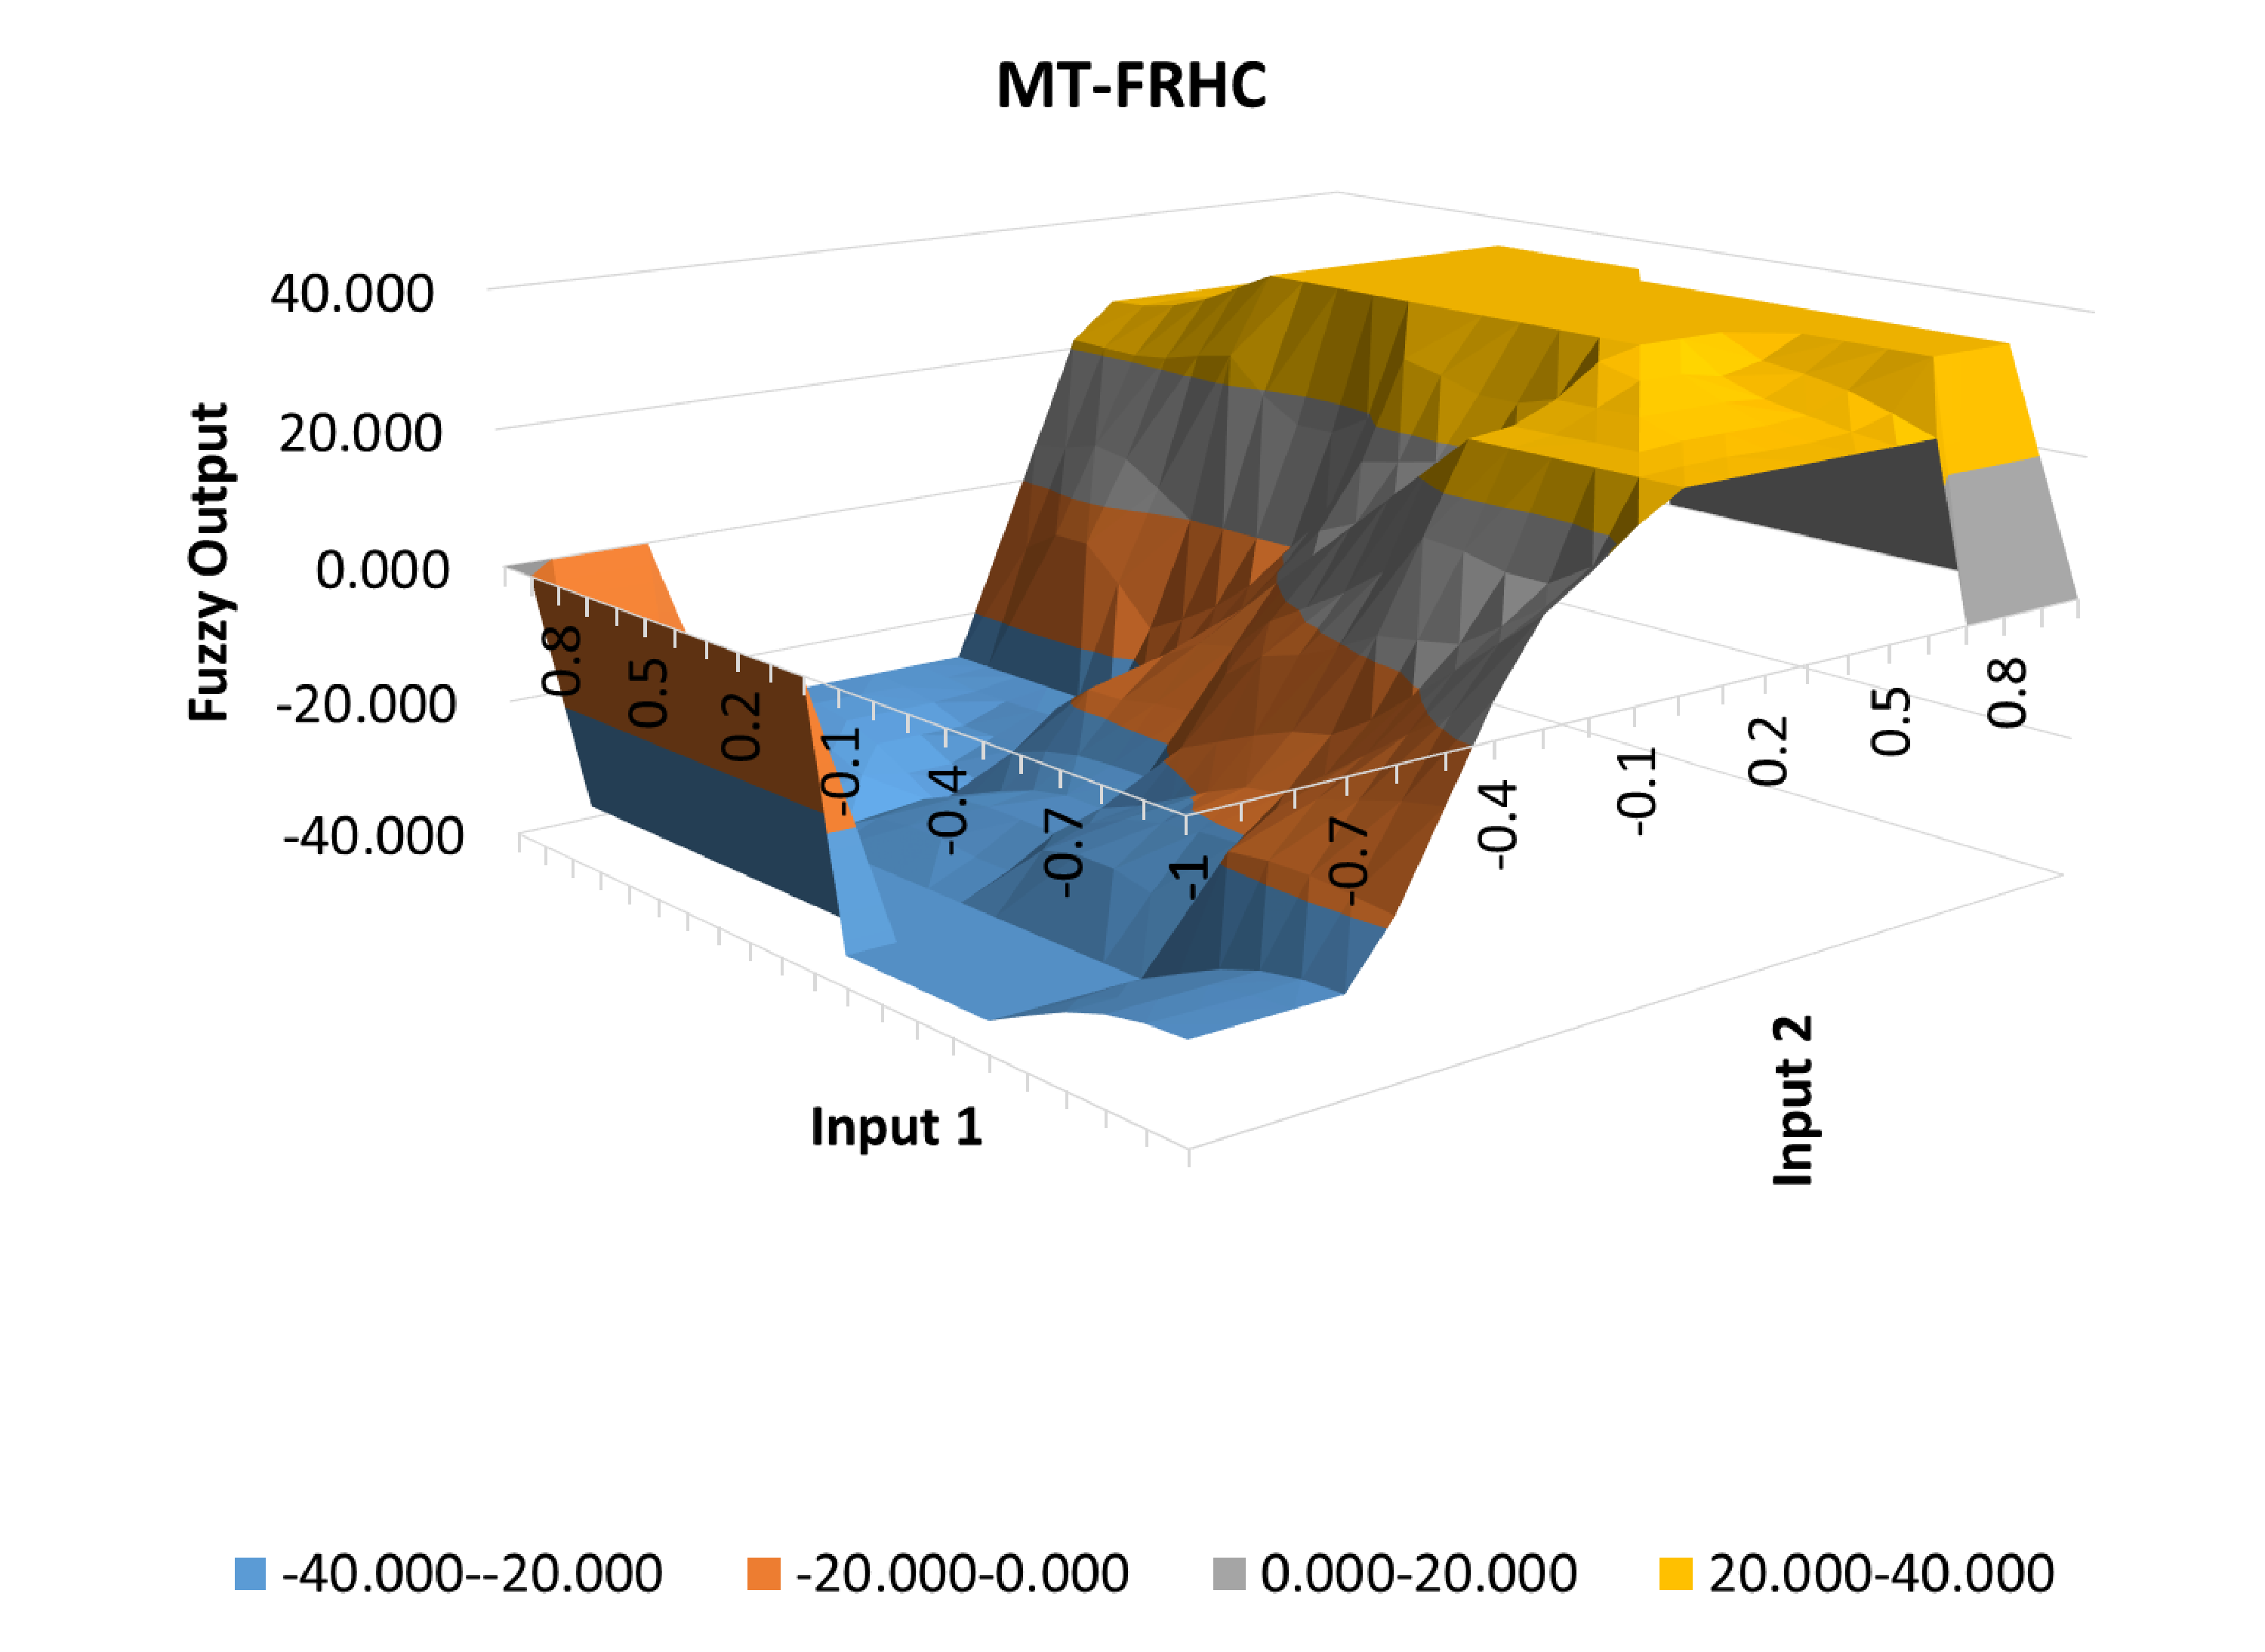
\includegraphics[width=0.6\linewidth]{Chapter2/chapter2/truck_MTFRHC.eps}} \\
	\subfloat[Truck Backer FIS: Matlab Fuzzy Toolbox]{\label{fig:SPlot_MFT_truck}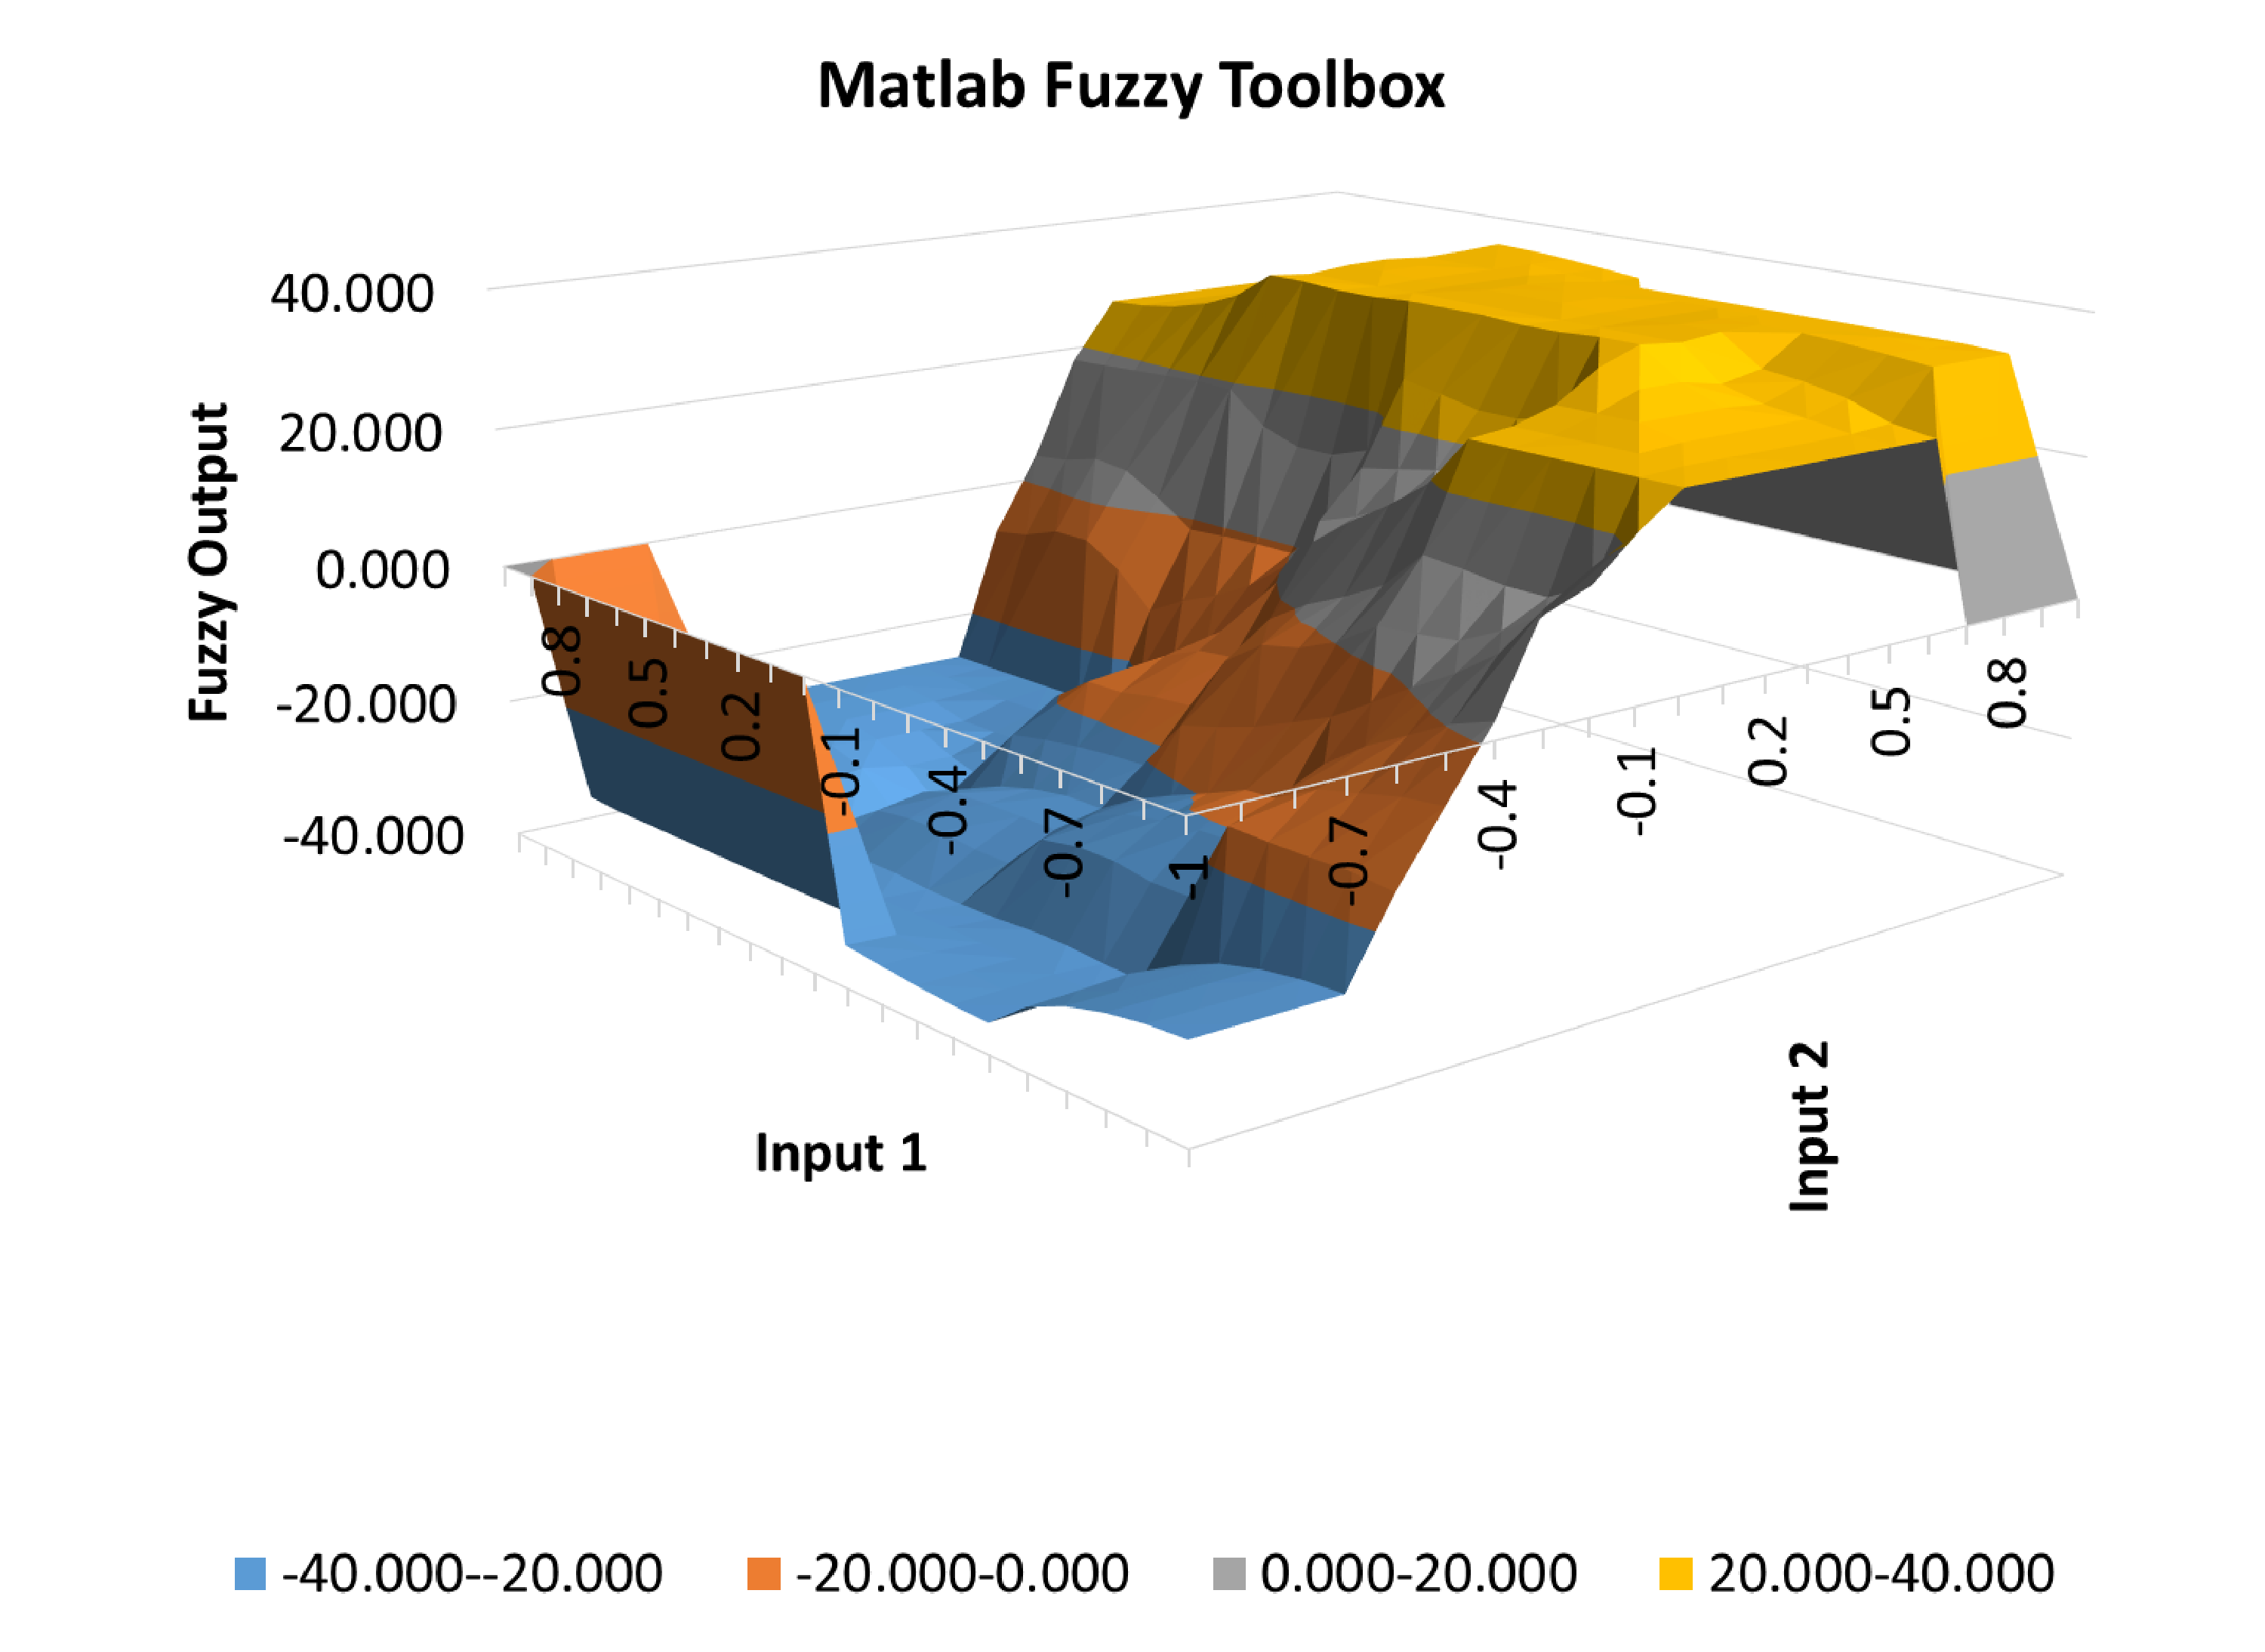
\includegraphics[width=0.6\linewidth]{Chapter2/chapter2/truck_MFT.eps}} \\ 
	\subfloat[Truck Backer FIS: Error Plot]{\label{fig:SPlot_Error_truck}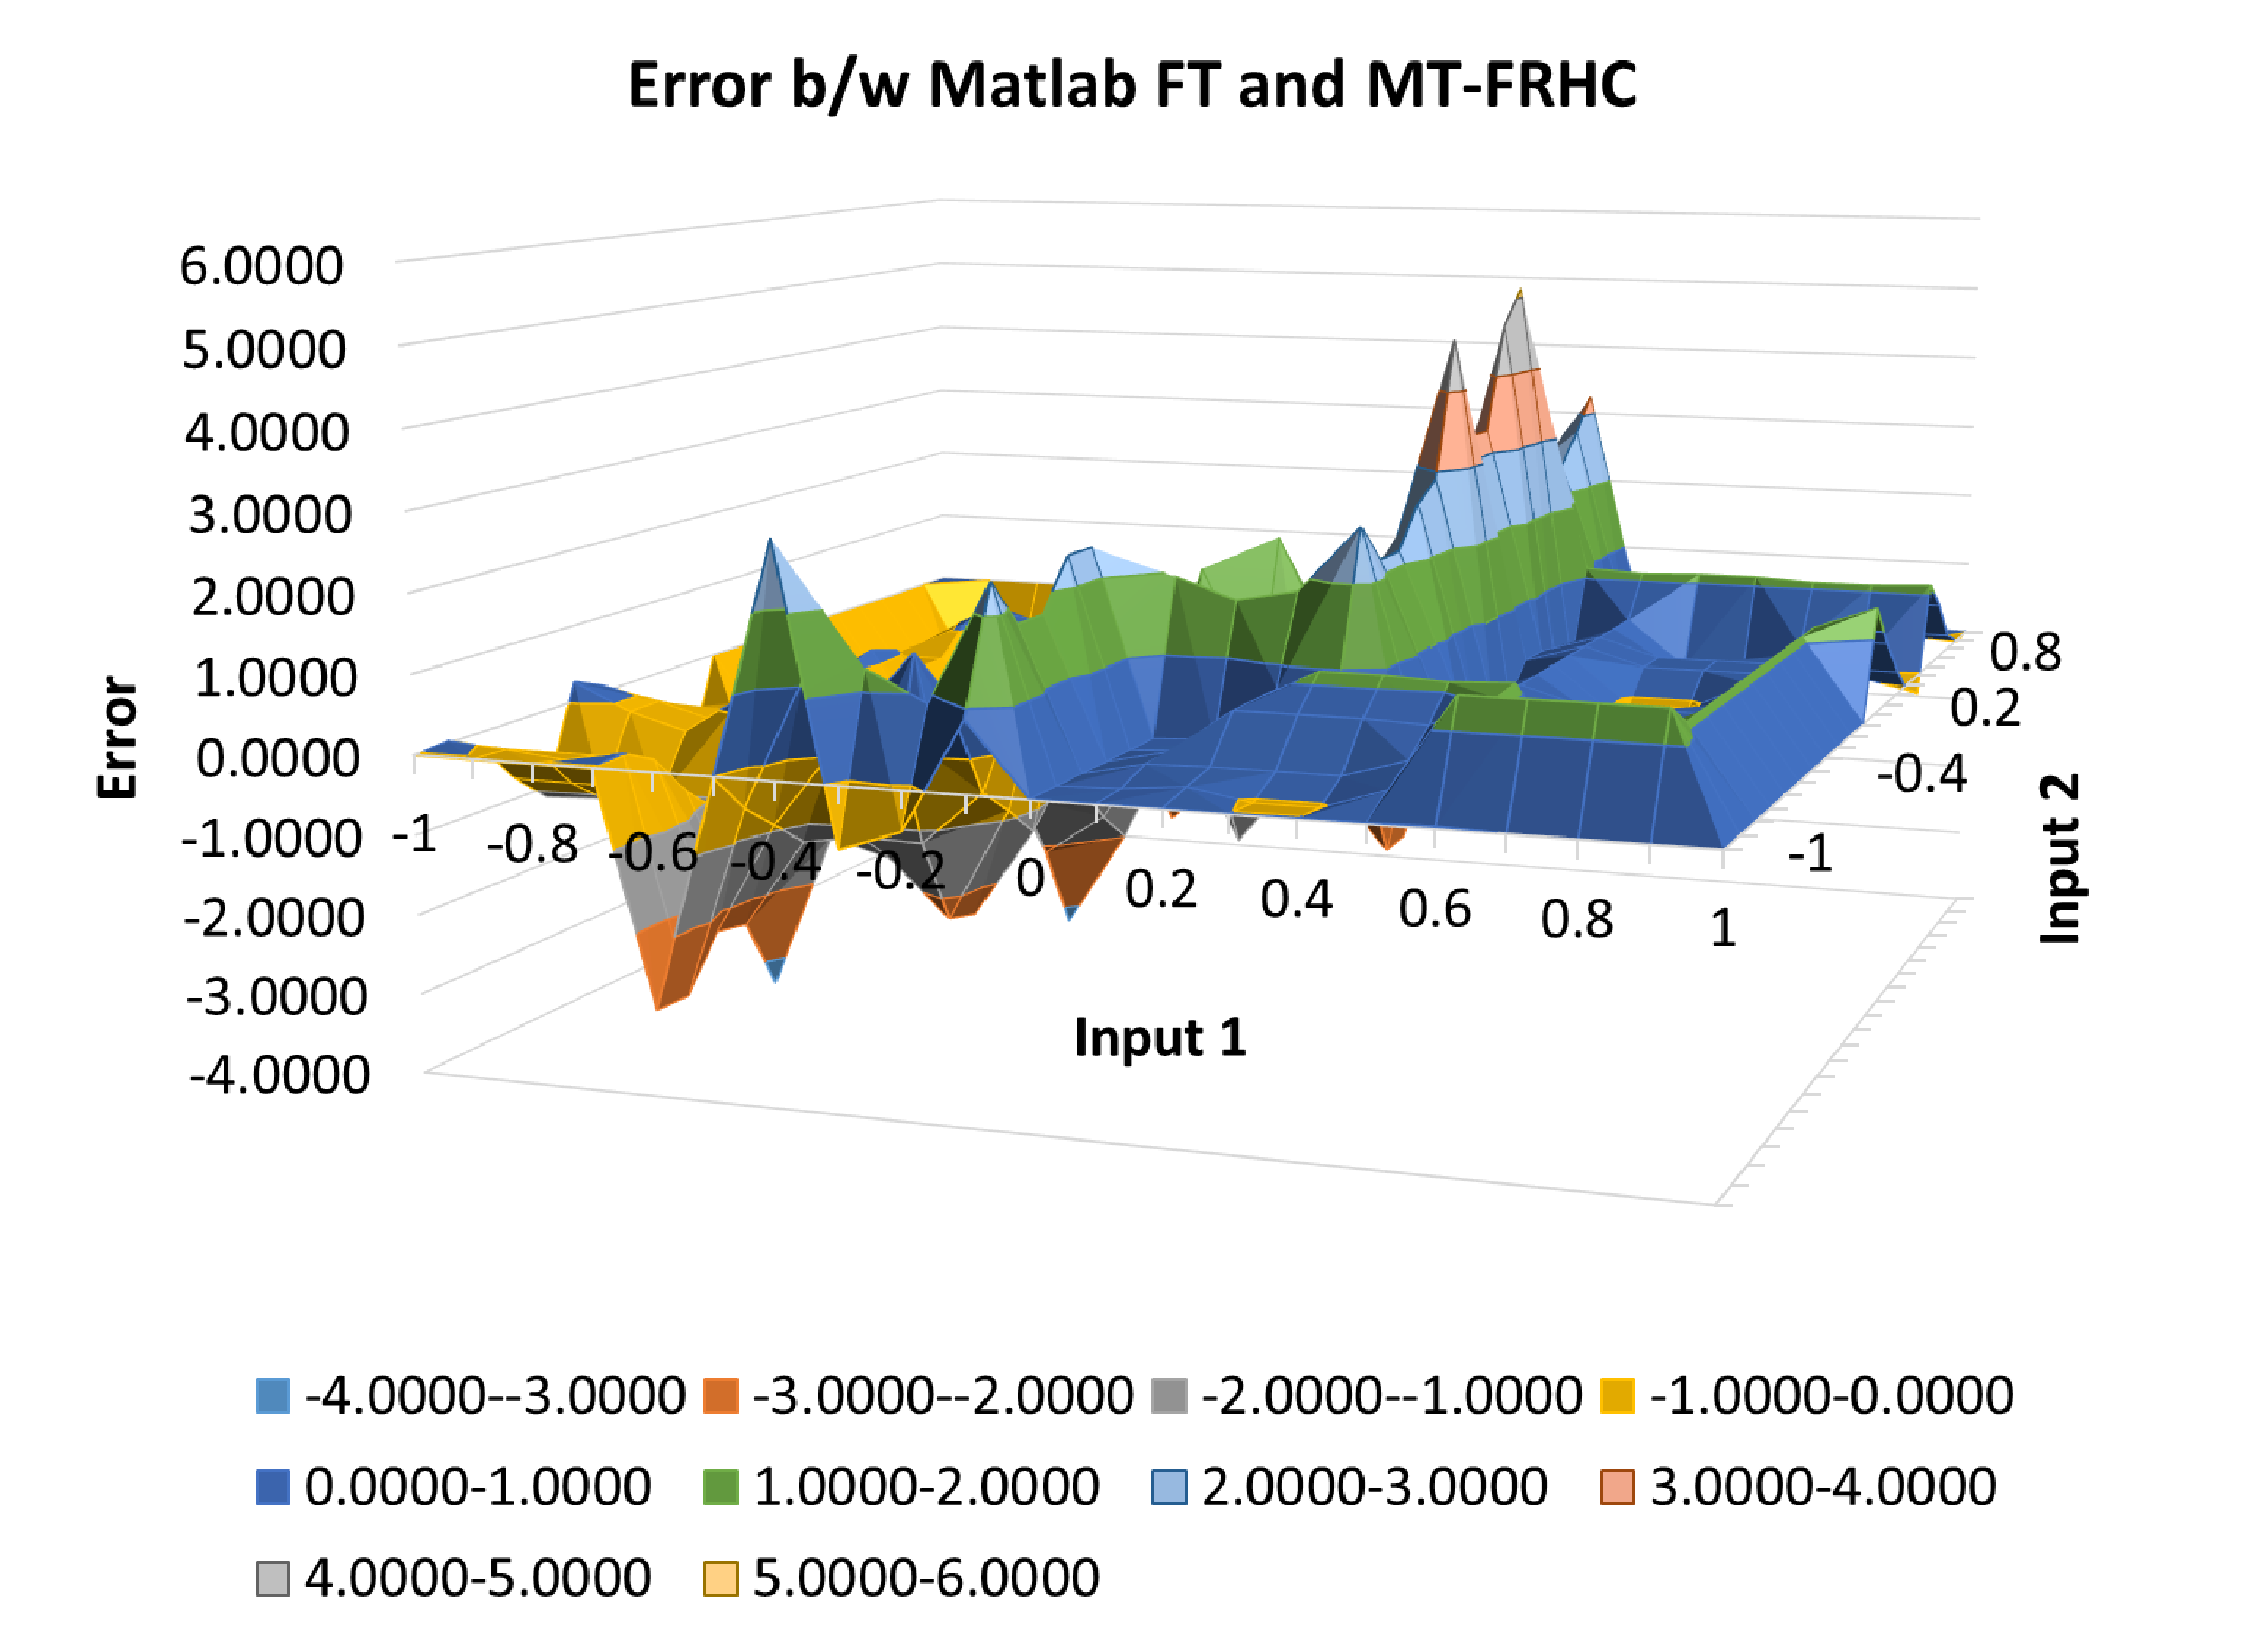
\includegraphics[width=0.6\linewidth]{Chapter2/chapter2/truck_Error.eps}}
	\caption{Surface Plot to test Fuzzy Inference Parameter for Fuzzy Inference Structure (FIS) used in Fuzzy PI approximation controller for Truck Backer Control \cite{Passino2010} }
	\label{fig:SurfacePlot_truck}
\end{figure}

\begin{figure}[h!]
	\centering
	\subfloat[Fuzzy PI Approximation to Control ACDC Motor]{\label{fig:MSEvTH_ACDC}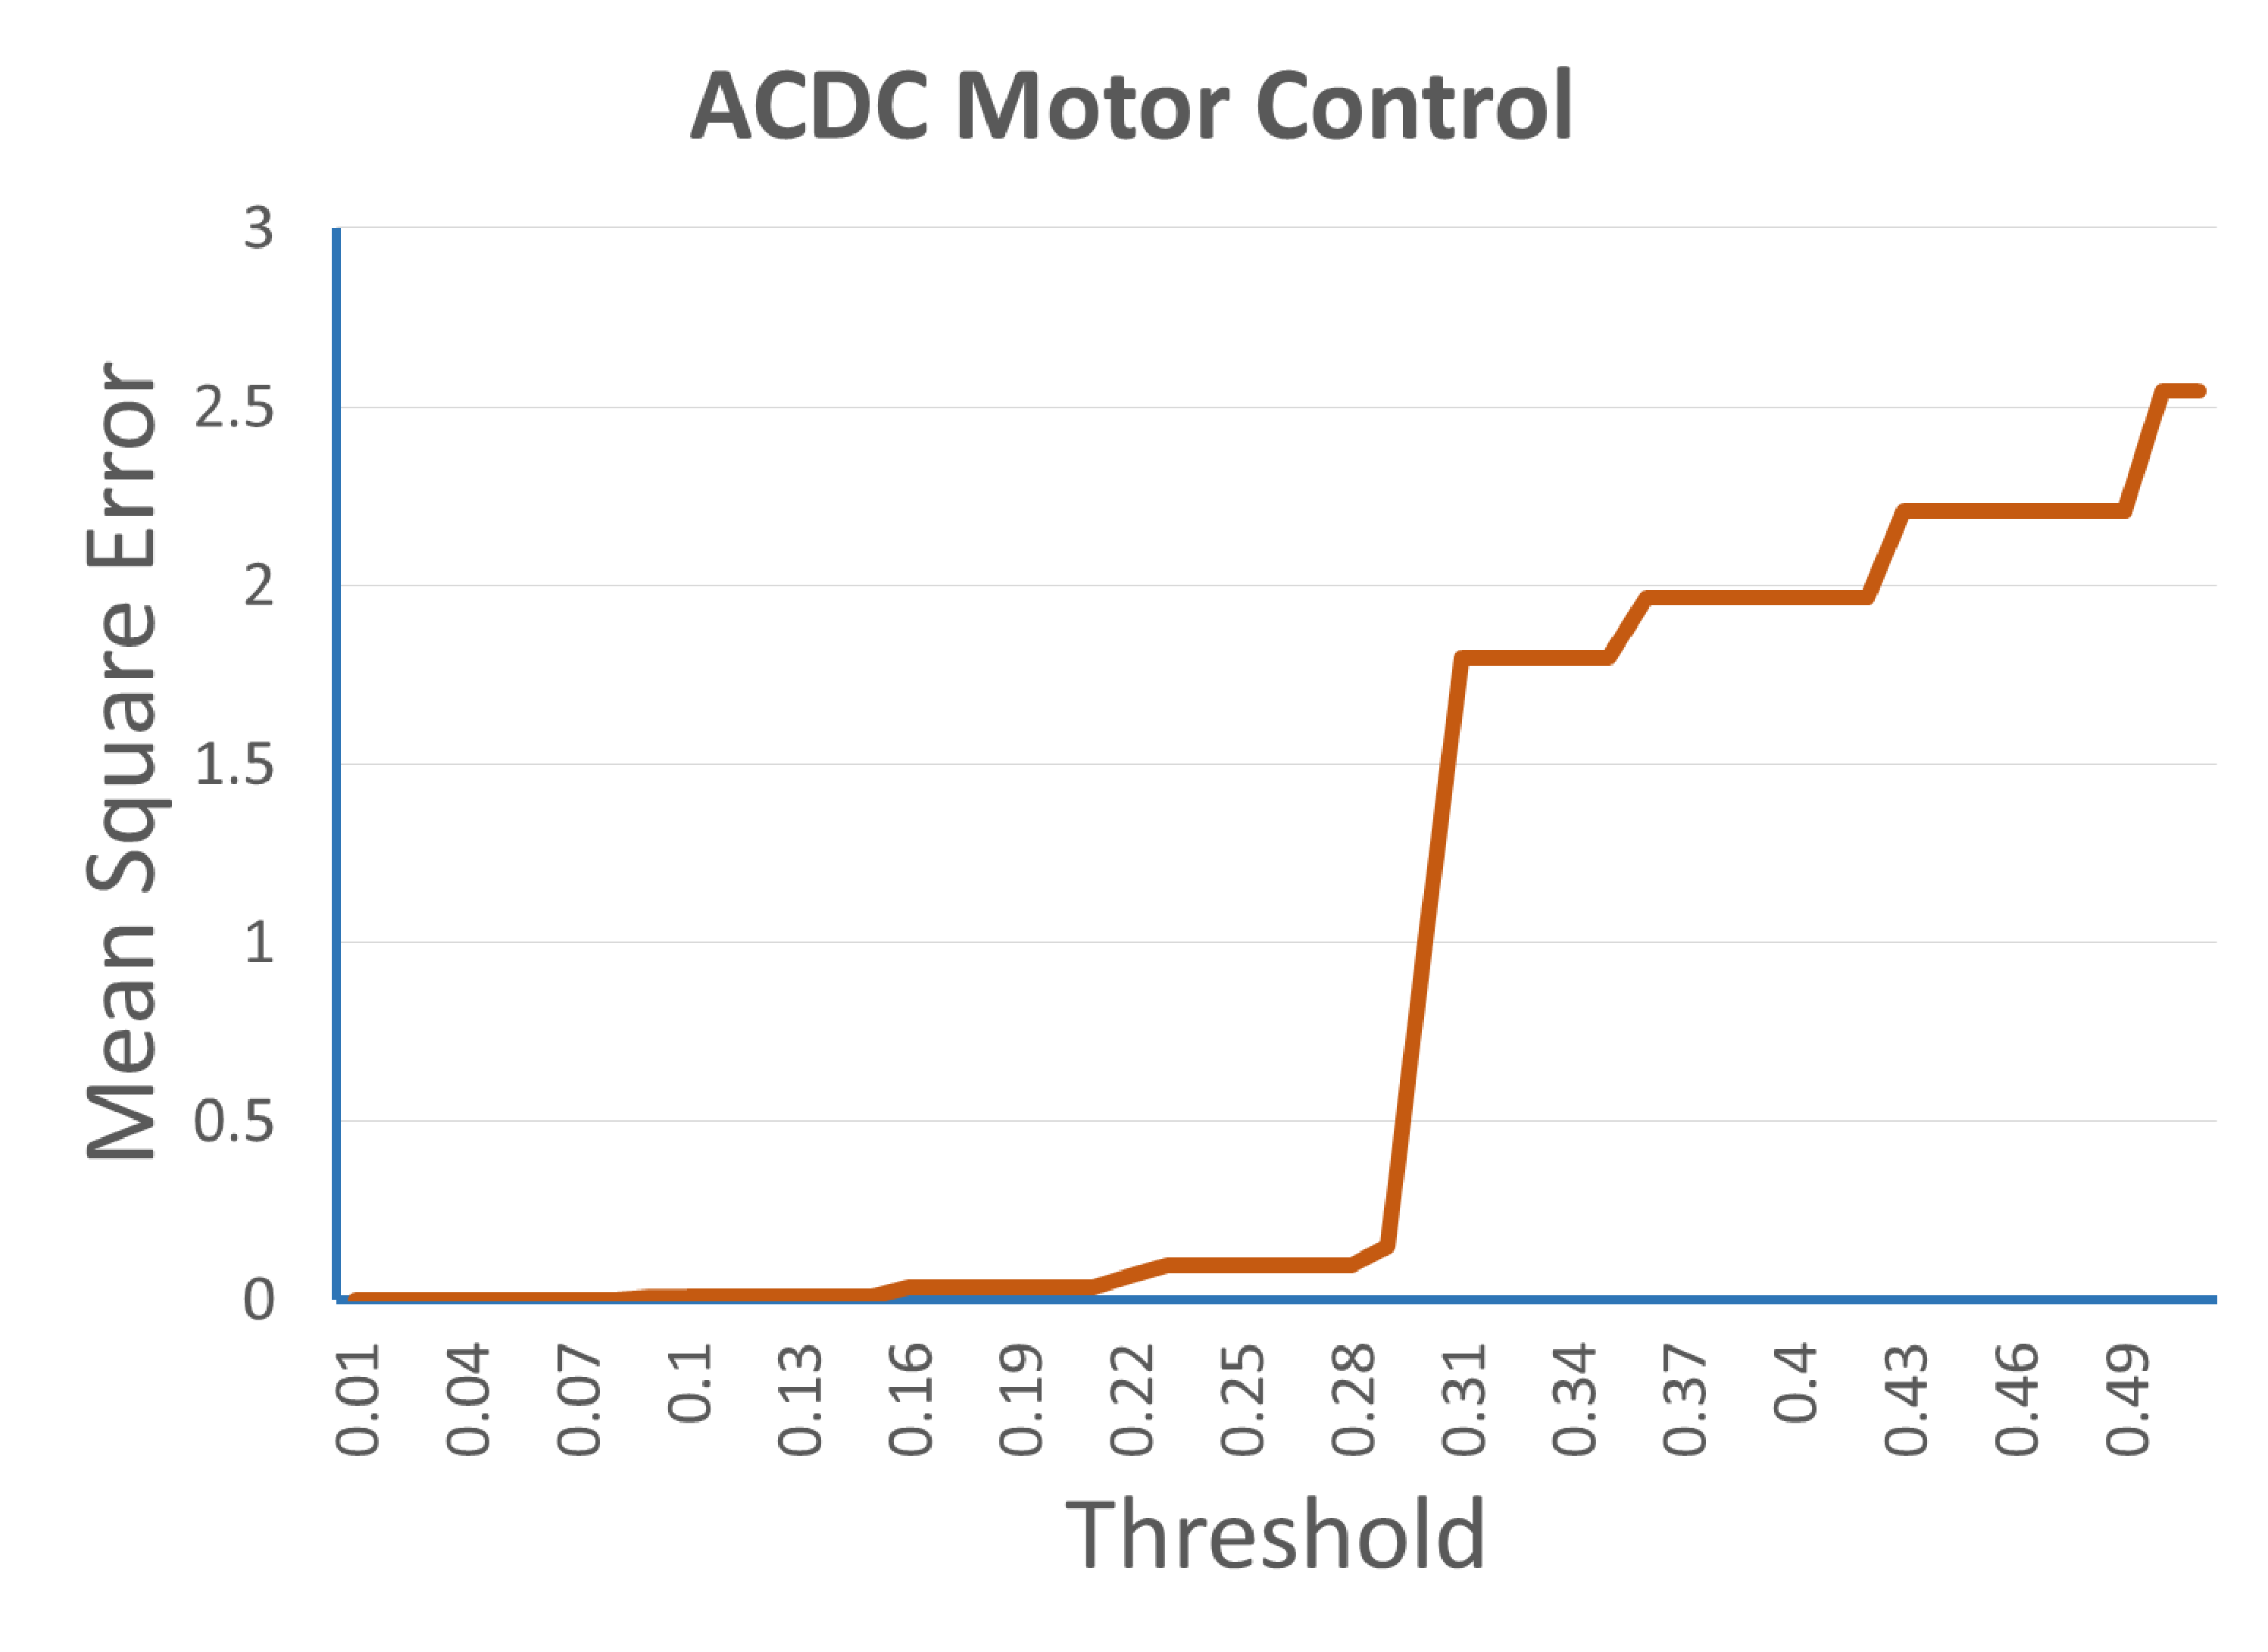
\includegraphics[width=0.55\linewidth]{Chapter2/chapter2/MSEvTH_ACDC}}\\
	\subfloat[Water Level Control of Two Tank System]{\label{fig:MSEvTH_Tank}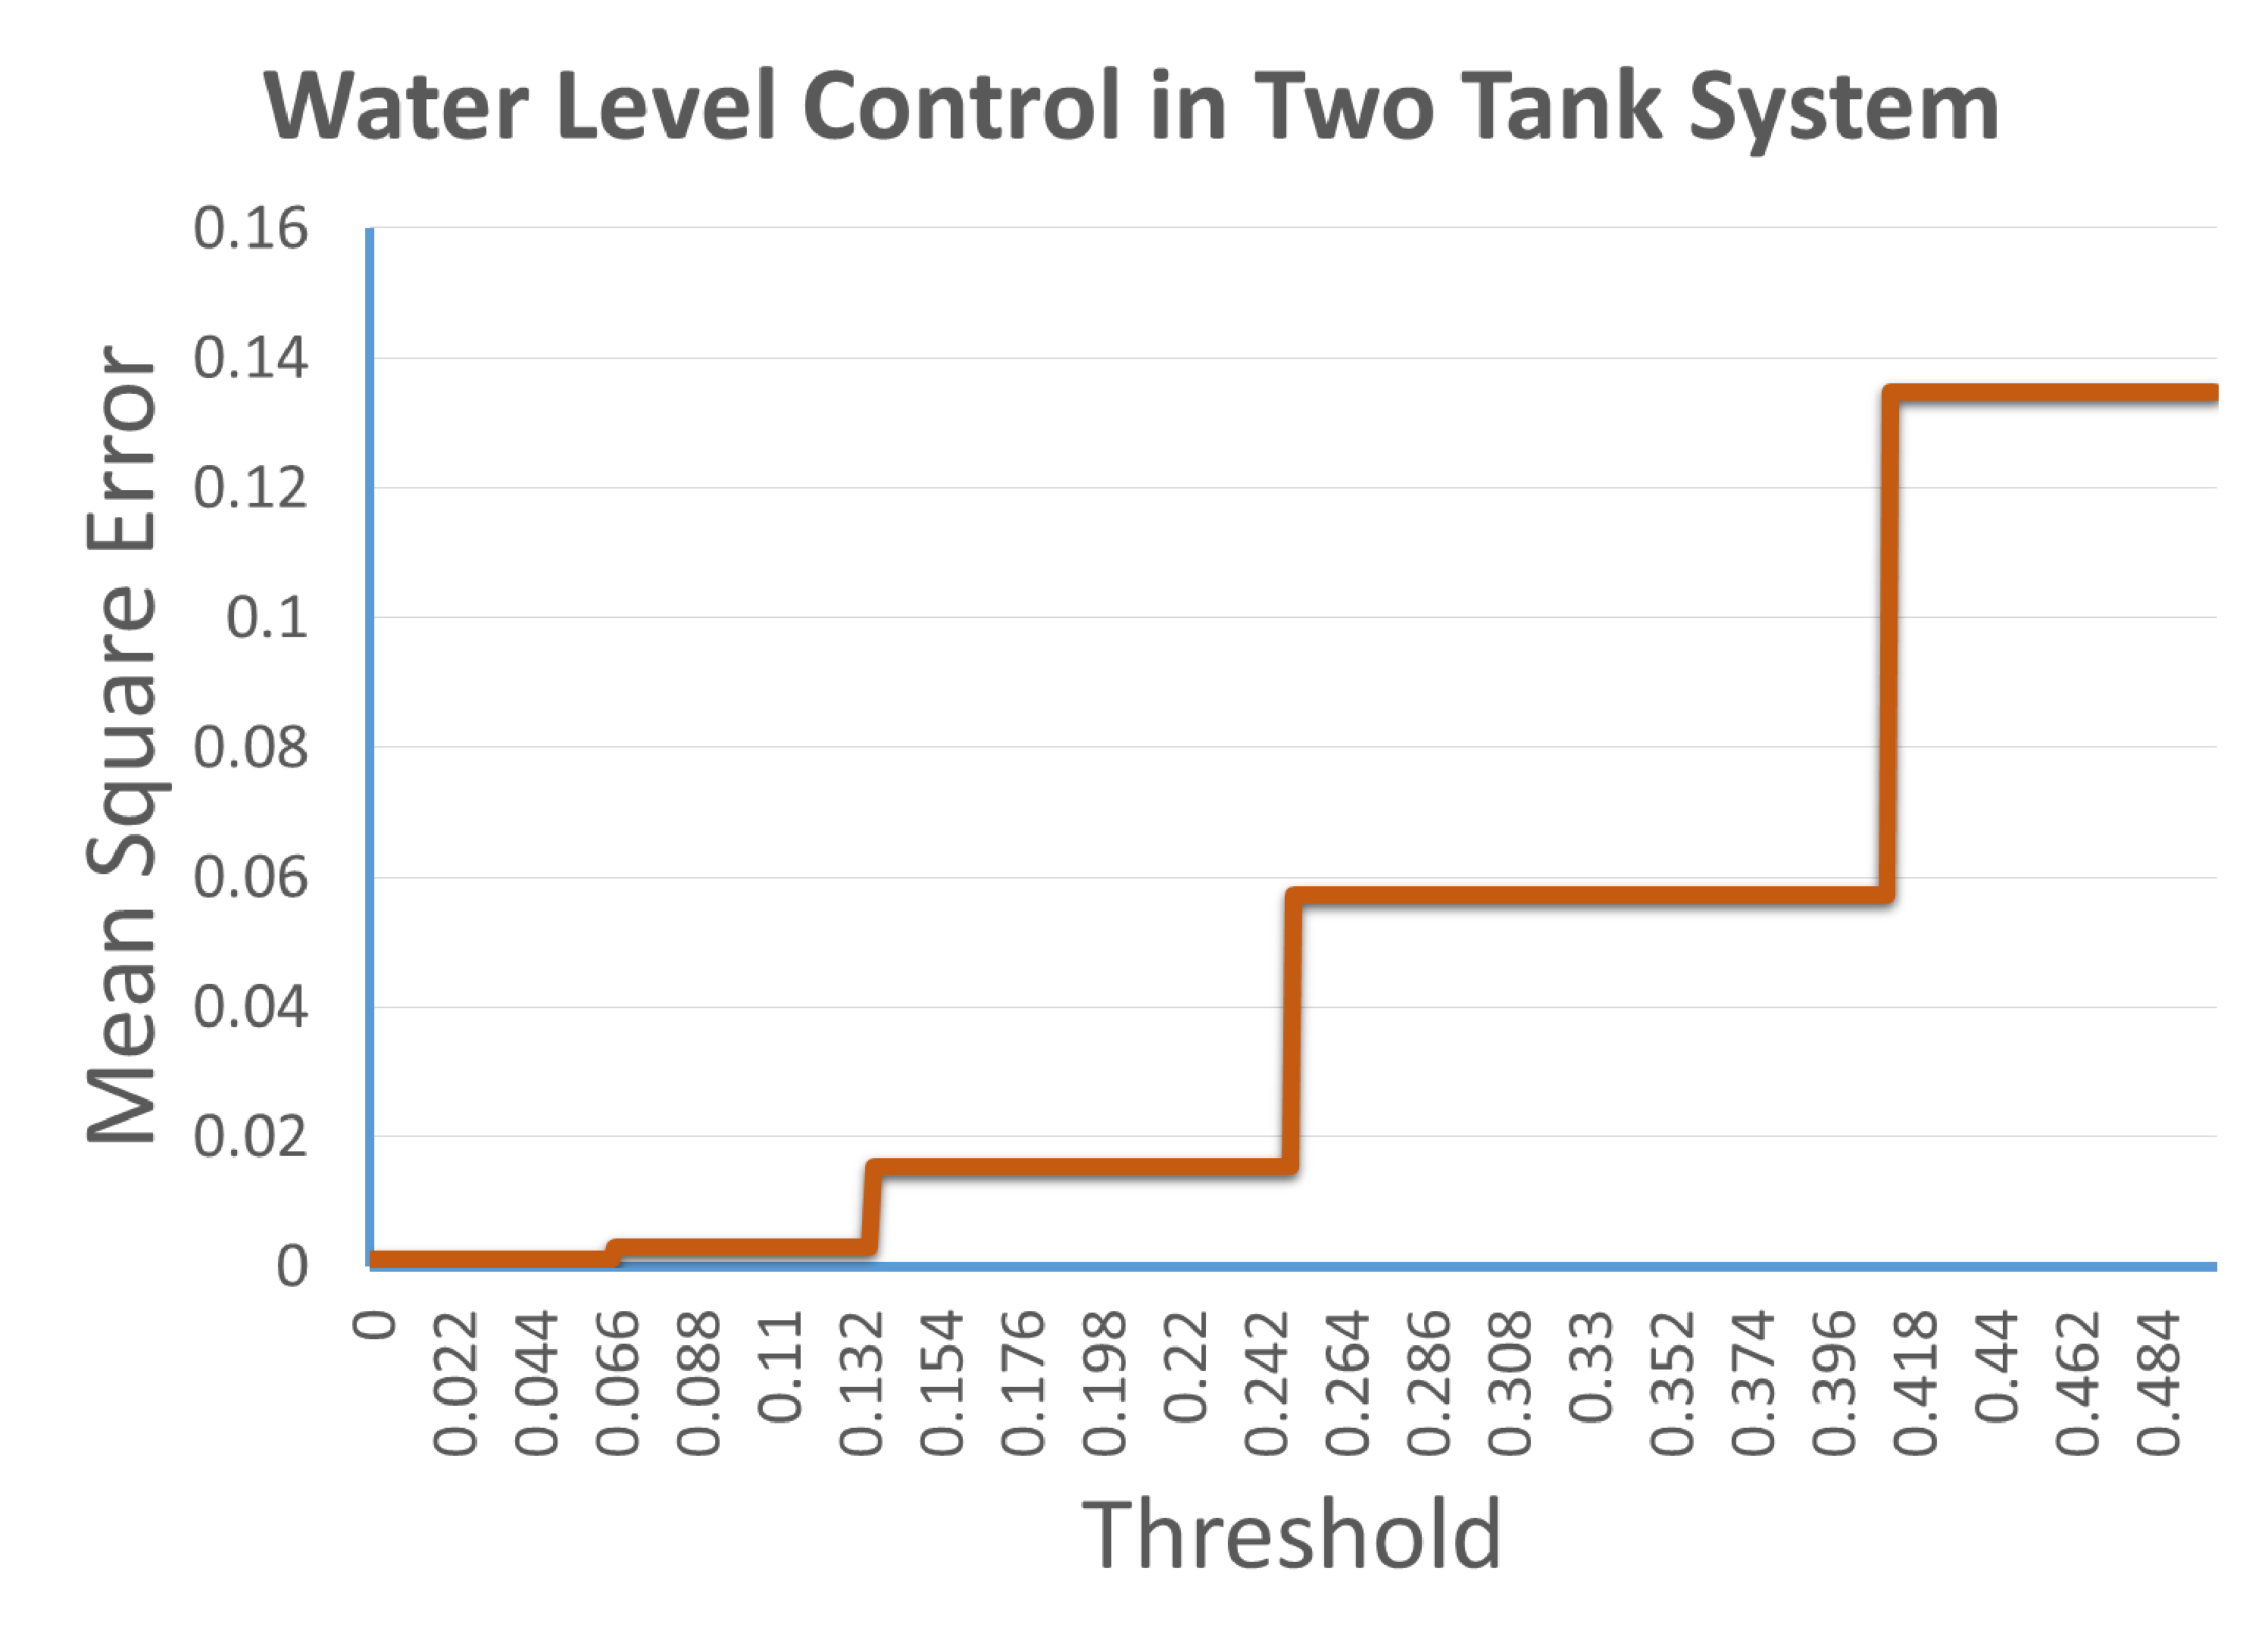
\includegraphics[width=0.55\linewidth]{Chapter2/chapter2/MSEvTH_Tank}} \\
	\subfloat[Truck Backer Control System]{\label{fig:MSEvTH_Truck}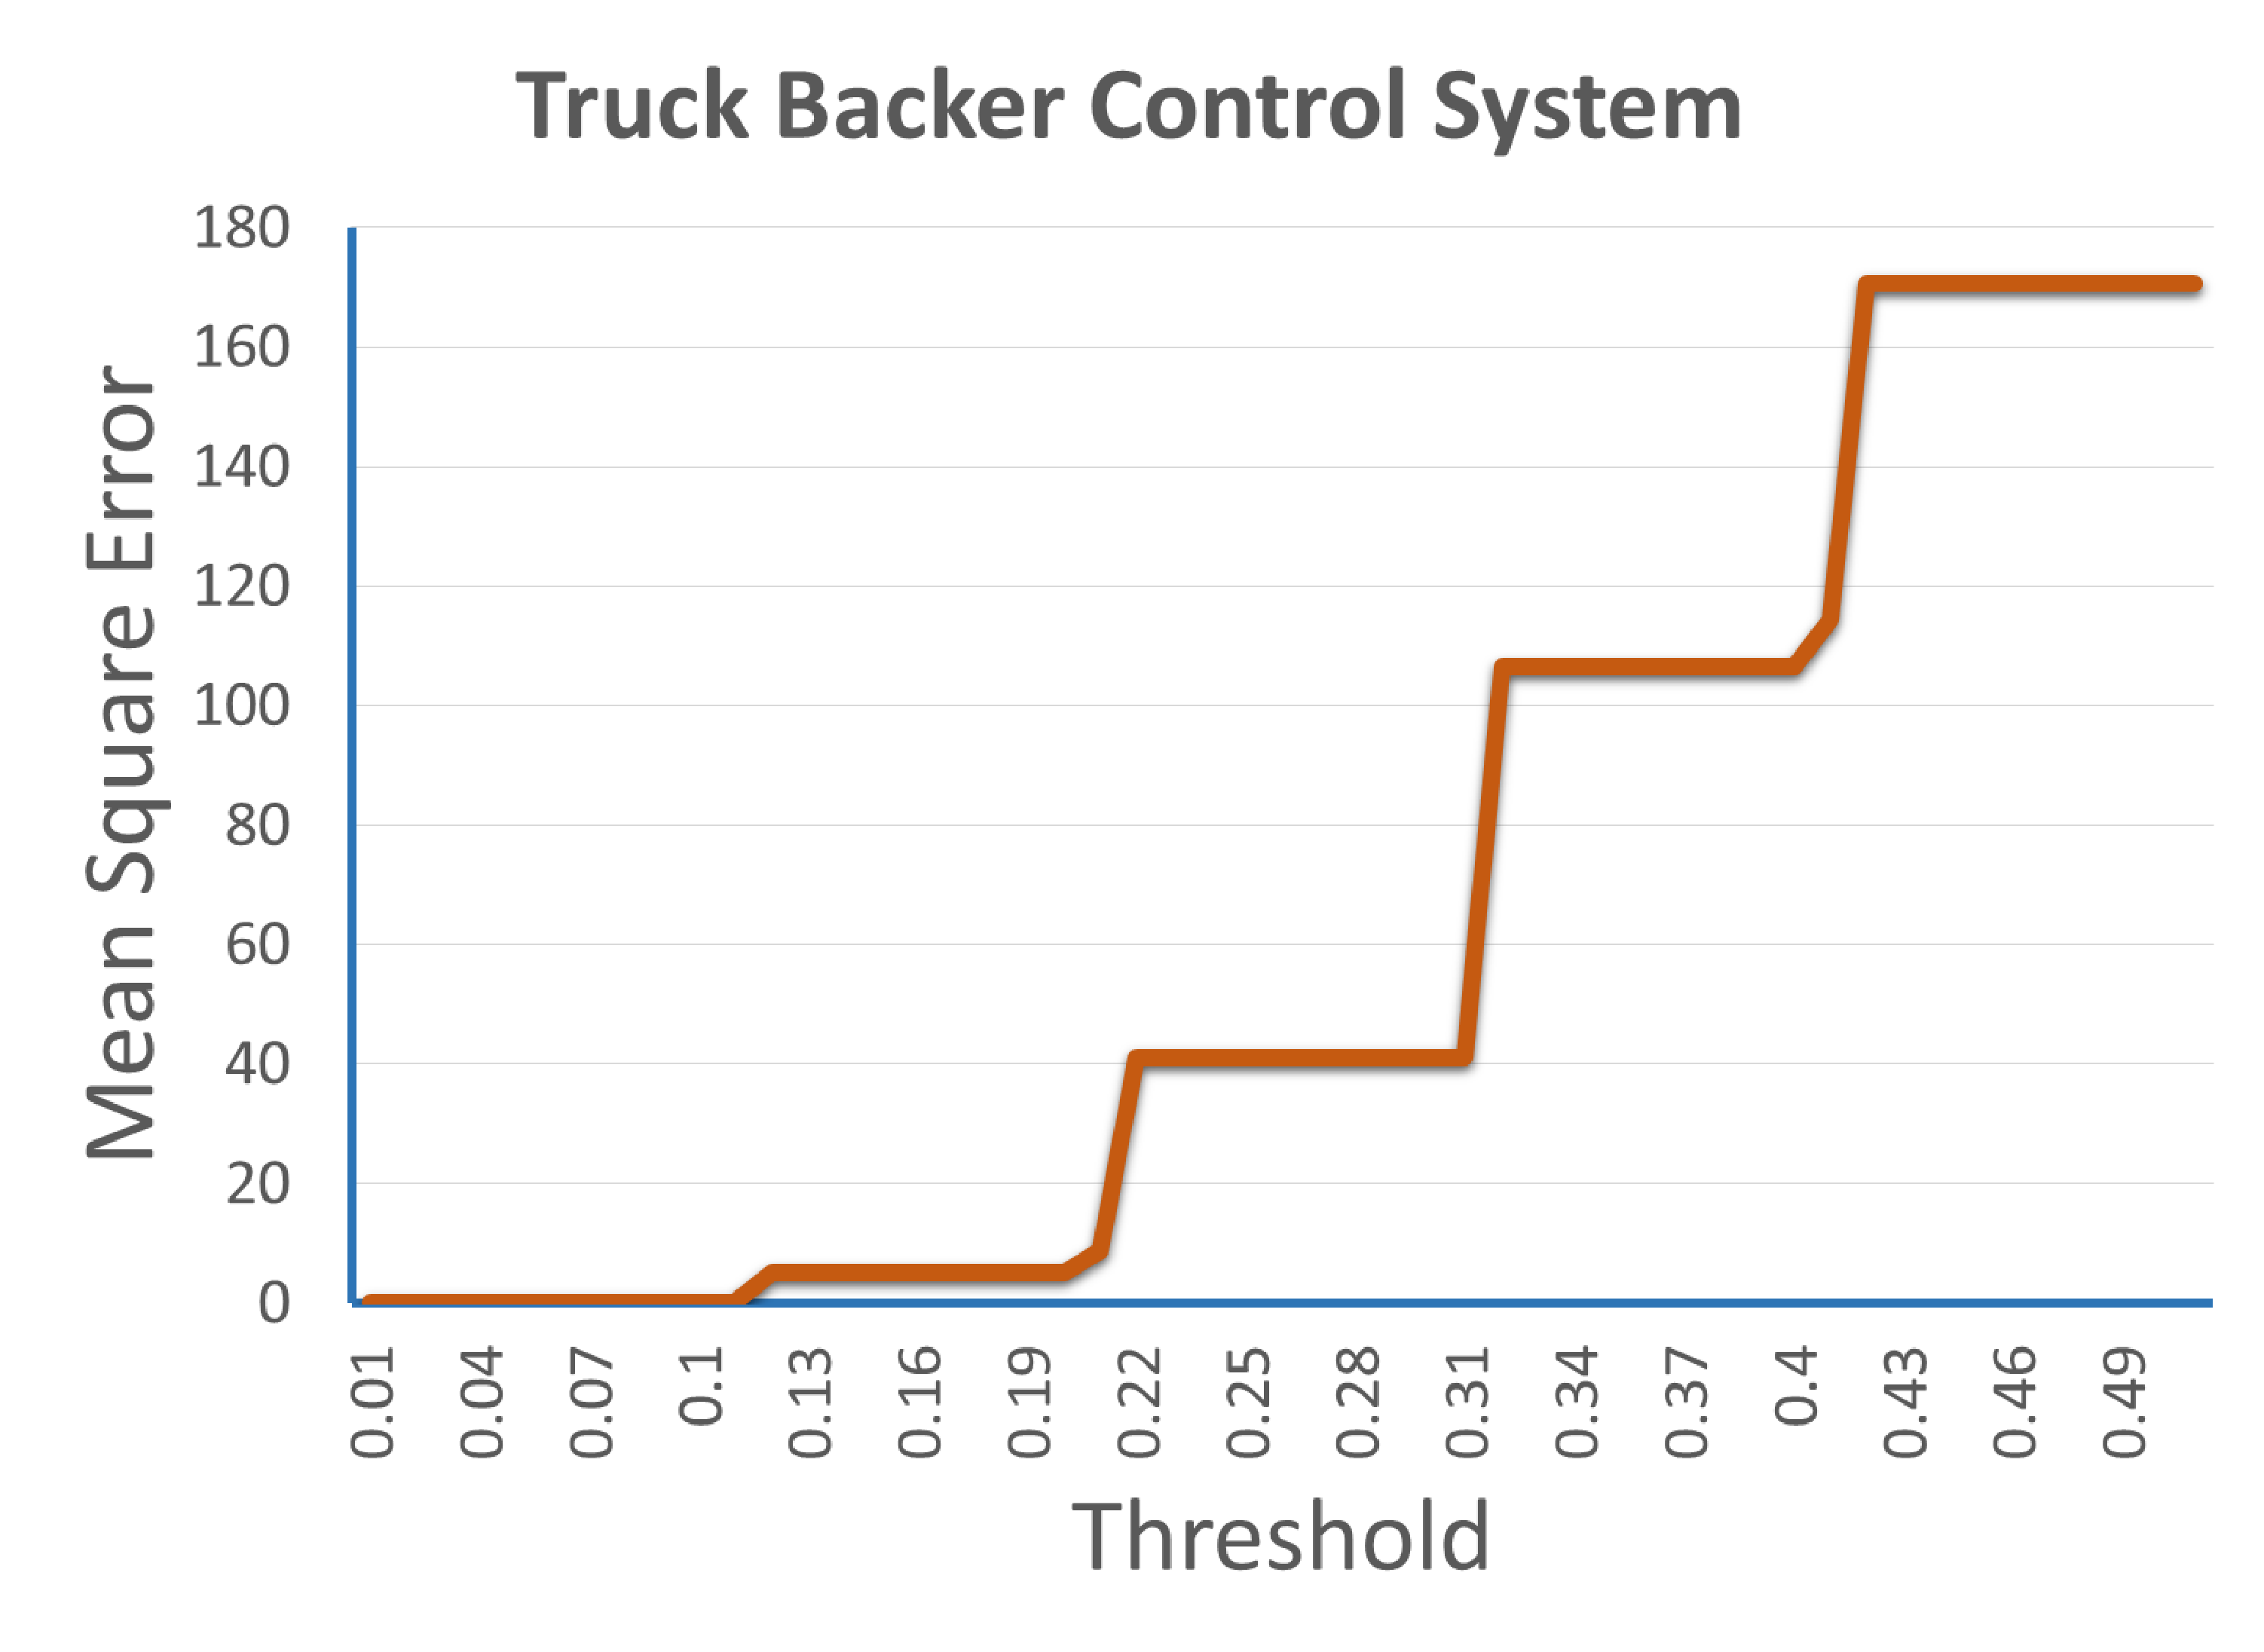
\includegraphics[width=0.55\linewidth]{Chapter2/chapter2/MSEvTH_Truck}}
	\caption{Dependency of MSE on threshold introduced in MT-FRHC Rule reduction technique for FIS structure file employed in FLC to control various systems. These systems considered are two input one output systems, no. of operations per inference is 16. }
	\label{fig:MSEvTH}
\end{figure}
In this section, the proposed MT-FRHC based G\hyp{}FLCS analyzed.  It is important to analyze the designed methodology on existing FLCS designs. Matlab Fuzzy Logic Toolbox (FLT) have been widely used to develop many fuzzy control applications. Every Matlab FLT uses a fuzzy parameter file called as \textit{fis} file which stores the FCP. In this analysis, the performance of the proposed MT-FRHC based G-FLCS is compared to Matlab FLT.

To analyze the performance of the proposed system, it was implemented on a test problem. Shiva Malla \cite{malla2012} used Matlab FLT to design a Fuzzy PI approximate controller for speed control of an Armature Controlled Direct Current (ACDC) motor. A web link to a FIS structure file used by Shiva Malla \cite{malla2012} for Fuzzy PI approximation to control ACDC motor is provided in Appendix-A. The Fuzzy PI Controller is a two-input one-output system with error and change in error ($\delta Error$) as the input and control signal as the output. The range of both the input space varies from $-1 $ to $ 1 $. he output ranges from $ -30 $ to $ 30 $. All possible combinations inputs with a step of 0.001 are sequentially introduced into the MT-FRHC based G-FLCS, and the correspond results are noted for threshold $ \tau = 0.2 $. A surface plot is generated from these observed results as shown in Figure \ref{fig:SPlot_MT-FRHC}. The x-axis represents the error ranging from 0 to 1 with a step size of 0.001, while the y-axis shows the change in error($\delta Error$) also ranging from 0 to 1 with a step size of 0.001. The output of the G-FLCS is plotted in the z-axis. Similarly, a surface plot is generated using Matlab FLT using the same FCP. This is presented in Figure \ref{fig:SPlot_MFT}. The individual error between these two system output is calculated and plotted in Figure \ref{fig:SPlot_Error}. The x and the y- axes, which represents the inputs remains same as in the other plots. However, the z-axis represents the absolute error between the system output generated from the proposed MT-FRHC based G-FLCS system and Matlab FLT. Considering Matlab MLT as the true value, it can be observed  MT-FRHC based G-FLCS produces a peak error of $ \pm 2 $ over an output range of $ \pm 30 $. At this moment, the proposed system produces a maximum of 6.67\% error.

The generality of a G\hyp{}FLCS can only be established once it is implemented on different FLCS designs. The proposed MT-FRHC based G-FLCS controller is tested similarly with two other benchmark control problems, namely, a water level control of a two tank system \cite{twotank2012} and a truck backer control system\cite{Passino2010}. Figure \ref{fig:SPlot_MT-FRHC_tank} shows the surface plot for output (on z-axis) of the MT-FRHC based G-FLCS system with respect to the water level (in x-axis) and input flow rate (y-axis). Figure \ref{fig:SPlot_MFT_tank} represents the surface plot for output (on z-axis) of the Matlab FLT system with respect to the water level (in x-axis) and input flow rate (y-axis). The surface plot of the error between these two systems is presented in Figure \ref{fig:SPlot_Error_tank}. It can be seen that for this particular example, MT-FRHC based G-FLCS produces a peak error of $ \pm 3\times10^{-15} $ over an output range of $ \pm 1 $. Now, the proposed system produces a negligibly small error that is very close to 0.

In Figure \ref{fig:SPlot_MT-FRHC_truck}, the surface plot for fuzzy output (on the z-axis) of the MT-FRHC based G-FLCS system is plotted for a truck backer system. Figure \ref{fig:SPlot_MFT_truck} represents the surface plot for fuzzy output (on the z-axis) of the Matlab FLT system for the same system. The surface plot of the error between these two systems is presented in Figure \ref{fig:SPlot_Error_truck}. It can be seen in error surface plot that, MT-FRHC based G-FLCS produces a peak error of $ \pm 5 $ over an output range of $ \pm 40 $. At this moment, the proposed system produces an error of 1.25\%.

Following the previous analysis, the same benchmark control problems were employed to draw dependency between the threshold $ \tau $ and mean square error.
It is analytically evident that MSE is proportional to the threshold $ \tau $. However, the computational complexity of G-FLCS is inversely proportional to $ \tau $. In an ideal scenario, a G-FLCS encounters following optimization problem.
\begin{itemize}
	\item Lower value of $ \tau $ to reduce MSE.
	\item Higher value of $ \tau $ to reduce computational complexity.
\end{itemize}
For MT-FRHC based G-FLCS, MSE is calculated with respect to Matlab FLT against different threshold values. In Figure \ref{fig:MSEvTH}, the trend of MSE with increase in $\tau$ is presented for Fuzzy PI Control of ACDC motor \cite{malla2012}, a water level control of a two tank system \cite{twotank2012} and a truck backer control system\cite{Passino2010}. It can be observed that MSE of a system is variedly dependent on different FIS structure file at the constant threshold. Thereby, it can be safely inferred that $\tau$ has to be dynamically assigned to a G-FLCS depending on the system it is employed, and this factor cannot be generalized. As a result of this, selection of $\tau$ should be based on
\begin{itemize}
	\item accuracy demand from the system
	\item throughput time of the system
\end{itemize}

\section{Proposed MT-FRHC based G-FLCS Implementation and its Validation}
At this juncture, it is necessary to implement the proposed algorithm on a programmable device and validate the results. To achieve this, the proposed system is implemented on a TI TMS320C6748 DSP processor operating on 300 MHz with $ \tau = 0.2 $. For comparative analysis of the MT-FRHC based G-FLCS technique, the Overlapping Membership Function (OMF) based G-FLCS is also implemented on the same platform. A 4-input/1-output, 9 rule, COA defuzzification FLC was used for testing. A download link to this FCP is provided in Appendix-A. The timing analysis of this experiment conducted is presented at Table \ref{tab:ch2timing}. Timing analysis of this experiment was executed using Code Composer Studio Timing Profiler. This tool presented the machine cycles consumed during execution of the method. 

\begin{table}[h]
	\centering
	\caption{Hardware Implementation: Timing Analysis}
	\label{tab:ch2timing}
	\begin{tabular}{cccc}
		\hline \noalign{\vskip 1mm} 
		Sl. & Cycles & Time (ms) & FLIPS \\ \hline \noalign{\vskip 1mm} 
		1. & 43370 & 0.1445 & 6920.42 \\
		2. & 38546 & 0.1285 & 7782.10 \\
		3. & 38451 & 0.1282 & 7800.31 \\
		4. & 38182 & 0.1273 & 7853.6 \\
		5. & 37567 & 0.1282 & 7800.31 \\
		6. & 30944 & 0.1032 & 9689.5 \\
		7. & 38995 & 0.13 & 7692.3 \\
		8. & 38513 & 0.1286 & 7788.2 \\
		9. & 38595 & 0.1287 & 7770.00 \\
		10. & 38578 & 0.1286 & 7776.05 \\ \hline
	\end{tabular}
\end{table}

From the Table \ref{tab:ch2avgtiming} it can be observed that the execution time for MT-FRHC is 0.0259 ms per inferences compared to Overlapping Membership Function (OMF) with 0.0346 ms per inference. This implies that the number of fuzzy logic inferences per second (FLIPS) completed by the proposed technique is quite higher. It has been found that the MT-FRHC based G-FLCS achieved 27 \% higher performance in terms of speed compared to the OMF based G-FLCS. Table \ref{tab:ch2avgtiming} presents the timing analysis of the individual modules in the G-FLCS. It can be seen that fuzzifier consumes significant machine cycles in comparison to other modules. This is mostly because the code has been written in a sequential manner, and there is a single thread of fuzzifier that fuzzifies crisp data from all four input channels to fuzzy data sequentially. The cycle time for fuzzifier can be significantly improved by invoking multiple threads using TI Sys/Bios\footnote{TI Sys/Bios is a real-time operating system primarily developed for TI manufactured DSPs, ARM and other programmable devices.} . 

\begin{table}[h]
	\centering
	\caption{Hardware Implementation: Average Time Response}
	\label{tab:ch2avgtiming}
	\resizebox{0.9\linewidth}{!}{%
		\begin{tabular}{ccccccc}
			\hline \noalign{\vskip 1mm} 
			~ & Fuzzifier & Inference & Defuzzifier & Total & Time & FLIPS \\ \hline \noalign{\vskip 1mm} 
			~ & \multicolumn{4}{c|}{(Cycles)} & \multicolumn{1}{c|}{(ms)} & (Kilo) \\ \noalign{\vskip 1mm} \hline \noalign{\vskip 1mm} 
			MT-FRHC & 29393 & 1823 & 6332 & 38548 & 0.1285 & 7.8 \\ 
			OMF & 41843 & 2198 & 8565 & 52606 & 0.1754 & 5.7 \\ \hline \noalign{\vskip 1mm} 
		\end{tabular}
	}
\end{table}


\section{Summary}
In this chapter, a theoretical analysis of M-FRHC and MT-FRHC has been elaborated which was aimed at countering the significant limitations of predominant FRHC technique. Simulation results indicate that the proposed scheme can be implemented on hardware G\hyp{}FLCS and replace the prevailing FRHC as rule reduction technique. This algorithm has managed to improve controller accuracy with a significant decrease in the computational complexity. This analysis portrays promising results in favour of MT-FRHC in both fronts and its utility in G-FLC design is dominantly inferred. This method also provides a platform where users can vary the number of overlaps and threshold value for fuzzifier of a G-FLCS in real-time. It has also been shown that with varying number of overlapping membership functions, the number of operations in the inference engine can be controlled. The introduction of threshold in fuzzifier will eradicate insignificant computations in the system. These programmable features in MT-FRHC provide added control on the performance of the controller itself and a user can steer the MT-FRHC based G-FLCS to the performance with better efficiency.
\chapter{System Architecture for MT\hyp{}FRHC based G\hyp{}FLCS}

\begin{chapterAbstract}{Preview}
	In this chapter we present a G\hyp{}FLCS architecture and its necessary modules and submodules. The chapter also provides a detailed explanation of a web based user interface for the proposed MT\hyp{}FRHC based G\hyp{}FLCS for reconfigurability. This hardware based fuzzy framework provides online reconfigurability of the system from remote location. However, it is important to note that there are over sixty flexible parameters that needs to be configured and it becomes an arduous task for an user to manage and configure them. Therefore, in this chapter we also introduce a genetic algorithm based parameter extraction technique. This technique helps to develop a course tuning and provide startup parameters which can be later fine tuned by the users remotely through the Web based User Interface. 	
\end{chapterAbstract}
\clearpage

\section{Introduction}
In previous chapter, a MT\hyp{}FRHC based Type\hyp{}I Mamdani G\hyp{}FLCS system is proposed and described.  As discussed briefly in Chapter 2, to counter uncertainty and variations in a nonlinear plant, adaptive control is extremely important. The adaptive control strategy maintains smooth performance of a system in the presence of these uncertainties by updating and tuning FCP at various time intervals. This is implemented in the proposed G-FLCS architecture by introduction of online and offline tuning methods. However, a theoretical analysis of the proposed MT\hyp{}FRHC rule reduction technique is essential before implementation of the tuning methods because the tuning parameters are strictly driven by the active rule reduction mechanism. Subsequently, these modules and submodules gets integrated with G\hyp{}FLCS and analyzed after implementation on a DSP hardware. Earlier in section \ref{sec:obj} it was discussed that \textit{Plug and Play Framework} and \textit{Runtime Tunability} is the essence of G\hyp{}FLCS design. To achieve these key features, it is important to integrate an interactive user interface with the G\hyp{}FLCS design. It is also imperative to formulate the system parameters in accordance to which the G\hyp{}FLCS is to be designed. There are large number of parameters in a Fuzzy Logic Controller. However, a truly generic fuzzy system is impractical because of the fixed resources for implementation. Therefore it is necessary to put an upper bound to each flexible parameter in the Fuzzy Control Parameters (FCP). Nevertheless, unlike most existing G\hyp{}FLCS designs, in this design the number of flexible parameters are not compromised to gain a higher speed. Rather other areas like optimization of code and algorithm is exploited to attain a desired speed and performance. It is also important to note that the FCP driving a G\hyp{}FLCS are generally programmed by users. There are large number of fuzzy parameters for an user to input in the G\hyp{}FLCS. This makes the process quite cumbersome. Hereby, a technique for automatic fuzzy parameter extraction from input\hyp{}output relationship of a process plant will grant the necessary ease of operation for an user. Therefore to start with the design of G\hyp{}FLCS, the system parameters are specified first. 

\section{G\hyp{}FLCS Parameters} \label{sec:des_op}

\begin{table}[b]
	\centering
	\caption{System Parameters}
	\label{tab:sysParam}
	\resizebox{0.65\textwidth}{!}{%
		\begin{tabular}{llc}
			\hline
			\noalign{\vskip 2mm} 
			\multicolumn{2}{c}{\textbf{Parameters}} & \textbf{Values} \\ \hline
			\noalign{\vskip 2mm} 
			\multirow{4}{*}{\textbf{Configurable}} & System Input & 1 to 4 (32 bits) \\
			& number of MFs per I/O & 2 to 7 \\
			& Shape of MFs & \begin{tabular}[c]{@{}c@{}}Triangular, GBell, \\ Trapezoidal, Gaussian\end{tabular} \\
			& Defuzzification Method & Centroid of Area \\ 
			& Rulebase & 2401 ($ 7^4 $)\\ \noalign{\vskip 2mm} \hline
			\noalign{\vskip 2mm} 
			\multirow{3}{*}{\textbf{Fixed}} & System Output & 1 \\
			& Method & MIN-MAX \\
			& I/O Signal Range & -5 to +5 V \\ \noalign{\vskip 2mm}  \hline
			
		\end{tabular}
	}
\end{table}
To start with the design of G\hyp{}FLCS, the system parameters are specified first. The FCP of proposed G\hyp{}FLCS is segregated into two segments namely configurable parameters and fixed parameters. Table \ref{tab:sysParam} presents the features of the proposed G\hyp{}FLCS. This table presents configurable and non\hyp{}configurable (fixed) parameters along with  order and variable values for a four\hyp{}input and one\hyp{}output system. Characteristics features of this architecture is as follows: 
\begin{itemize}
	\item A 32 bit precision Input and Output is considered.
	\item A web based user interface (WebUI) to remotely acquire fuzzy parameters. 
	\item Wide range of output MFs tuning consisting of singleton, triangular, trapezoidal, Gaussian and GBell type membership functions.
	\item MIN\hyp{}MAX Inference with full set rules.
\end{itemize}
This controller was implemented on a TI C6748 DSP processor. The major reasons for using DSP are:
\begin{itemize}
	\item DSP provides an effective implementation of multiplication and accumulation (MAC) and this helps in efficient COA implementation.
	\item File handling and socket programming is an integral part of this design. These were achieved easily since the development is in C language.
	\item This design supports high level of branching and decision making.
\end{itemize}	 

\section{System Architecture of Proposed G\hyp{}FLCS}
The proposed system architecture involves hardware\hyp{}software co\hyp{}design to present a complete reconfigurable G\hyp{}FLCS as shown in Figure \ref{fig:ProposedFLCArchitecturalDesign} and Figure \ref{fig:ProposedGenericFuzzyLogicSystemArchitecture}. In Figure \ref{fig:ProposedFLCArchitecturalDesign}, a graphical abstract of the overall system is represented. It can be observed that the controller is interfaced on one side in a feedback loop with the plant and on other side with the users through a client\hyp{}server based interface. The client\hyp{}server model allows reconfigurability of the system from remote locations. Figure \ref{fig:ProposedGenericFuzzyLogicSystemArchitecture} presents the internal architecture of the G\hyp{}FLCS design.  

The WebUI in client server model represents the software and the driver layer to interface the hardware G-FLCS through serial port to the server. The DSP hardware receives FCP data serially and stores them in predefined memory locations. These parameters are segregated in two categories namely \textit{Setup}  parameters and \textit{Rulebase} data. The driver layer in the hardware G\hyp{}FLCS receives and acknowledges the data transmission. 
A WebUI drives the proposed hardware G\hyp{}FLCS storing FCP data in a file in specific format. The file is shown in Appendix-A. It may be noted that the FCP file is generated deliberately in accordance with Matlab Fuzzy Inference System (FIS) file format to provide liberty to integrate a parameter data file generated using Matlab Fuzzy Logic Toolbox as well. Submitting the parameters triggers a desktop application that is native to the server. Objective of this program is to transmit the FCP from database to the hardware G\hyp{}FLCS through serial communication. The FCP data is stored in the DSP board based according to a predefined memory map. G\hyp{}FLCS designed with MT\hyp{}FRHC rule reduction scheme, operates on the inputs with these FCP data to provide desired control action. Fuzzifier, inference engine and defuzzifier is programmed with information about the data and its corresponding memory location. With these information, fuzzifier transforms crisp inputs in fuzzy domain and a Mamdani inference engine, coupled with the Rulebase in the system memory produces fuzzy output. Defuzzifier transforms the fuzzy output compiled by the inference engine to provide crisp output. There are various types of defuzzifier but in this work centroid of area (COA) is used considering its popularity and effectiveness. 

%Offset address \textbf{0000}H to \textbf{00D6}H in Table \ref{tab:memorymap} shows the details of Setup parameters. \textit{Rulebase} parameters appear in memory location \textbf{00D7}H to \textbf{1D0C}H which is reserved to store \textbf{{2401}\footnotemark} ~rules.
%\footnotetext{Maximum number of rules that this design can support is ($ = 7^4 $) since there can be maximum of 7 MFs for maximum of 4 Inputs.} 
\begin{figure}[h!]
	\centering	
	\subfloat[System Architecture]{\label{fig:ProposedFLCArchitecturalDesign}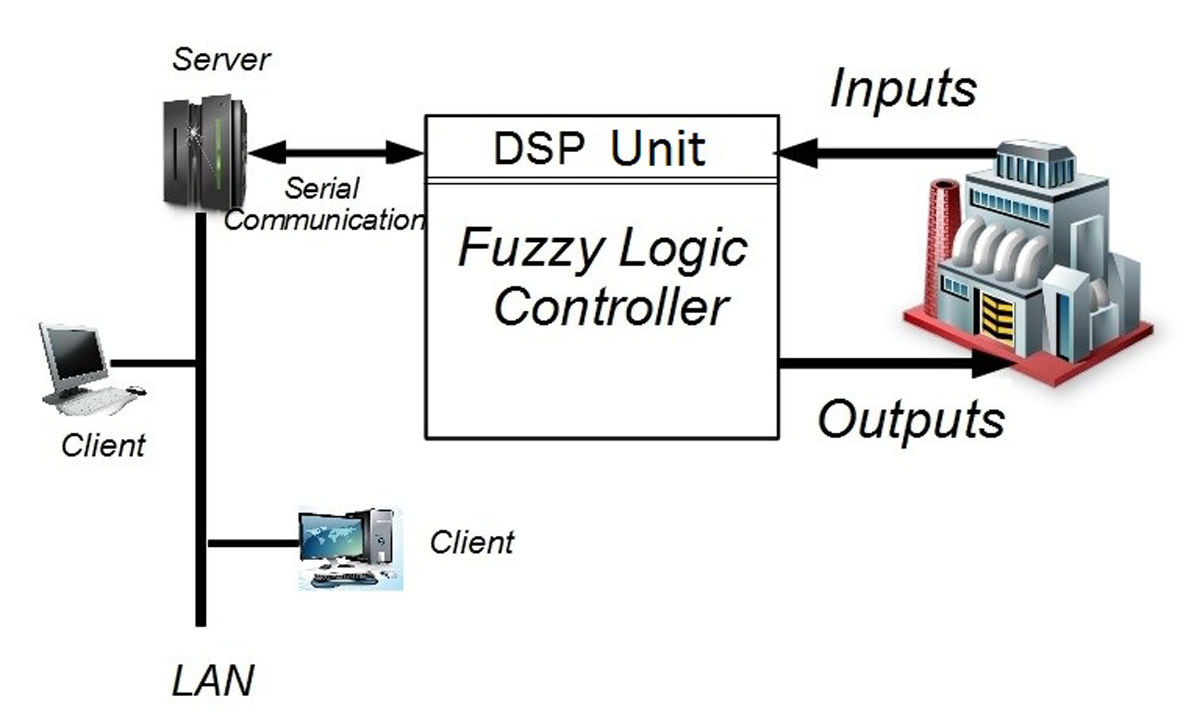
\includegraphics[width=0.9\linewidth]{Chapter3/chapter3/Fig1.eps}} \\
	\subfloat[Hardware Design]{\label{fig:ProposedGenericFuzzyLogicSystemArchitecture}\includegraphics[width=0.9\linewidth]{Chapter3/chapter3/Fig2.eps}} 
	\caption{Proposed G-FLCS Design Architecture}
	\label{fig:sysArch}
\end{figure}
\section{Development of a Client\hyp{}Server Model User Interface} \label{sec:WebUI}
A client\hyp{}server model is widely used for data transfer over large distance. Computer applications like are Email, network printing, and the World Wide Web use client–server model for data exchange. It is reliable, fast and secured distributed application structure. In the proposed design, it is cardinal to have a distribution structure over which users from large distance can operate the controller. 
\subsection{client\hyp{}server Model}
The client\hyp{}server model, also known as server\hyp{}client model, is a computing model developed on distributed computing structure. This structure segregates workload between a centrally connected service provider (\textit{Server}) and the various service users (\textit{Clients}) \cite{Simon2006}. Its is a standard model for developing network applications. The \textit{Server} process starts the computing module by initializing itself. Once the initialization protocol successfully completes, it goes to sleep and waits for incoming client requests. \textit{Client} processes can initiate from any system in the network including the host system running the \textit{Server} process. Once a service request is attended, this \textit{Server} application goes back to sleep and awaits incoming requests. 
Server applications or processes are of two types.
\begin{itemize}
	\item \textbf{Iterative:} In these type of applications, a single copy of the server application executes to service only a single user at any time. While a user request is attended, other users have to wait. These applications are developed when prior knowledge about the time to service individual request is present. 
	\item \textbf{Concurrent:} These \textit{Server} applications provides service to multiple users at any time. When a user requests for a service, the \textit{Server} application replicates a copy of itself which dedicatedly serves that user. This process repeats for every incoming service requests from the \textit{Clients}. These applications are developed when prior knowledge about the time to service individual request is absent.	
\end{itemize}
The client\hyp{}server model of communication developed for hardware G-FLCS uses TCP. TCP is an important protocol of TCP/IP networks where it helps to establish connection and exchange data. Establishment of a connection between two hosts depends upon five components
\begin{itemize}
	\item Protocol used
	\item Source IP address
	\item Source port number
	\item Destination IP address
	\item Destination port number 
\end{itemize}
With proper set of information, a connection between two hosts is established.

\subsection{ASP.NET and development of WebUI}
In this work, ASP.NET has been extensively used to develop the WebUI for hardware G-FLCS. This web application is designed with an intention to develop an user interface which, once installed on a central server, can be accessed over Internet to provide remote reconfigurability to the proposed hardware G-FLCS. The framework behind this application is demonstrated pictorially in Figure \ref{fig:fig3_9}. The figure shows that Microsoft IIS7 hosts and web application and interfaces it to the internet. Users from different location can access this application. Standard IP protocols are used for the WebUI for hardware G-FLCS as stated in Table \ref{tab:protocols}
\begin{table}[t]
	\centering
	\caption{TCP/IP Communication Layers and their Protocols}
	\label{tab:protocols}
	\begin{tabular}{ccc}
		\hline SL. No. & Layer & Protocol \\ 
		\hline 1. & Data Link Layer & Ethernet \\ 
		2. & Network Layer & IP \\ 
		3. & Transport Layer & TCP \\ 
		4. & Application Layer & HTTP \\ 
		\hline 
	\end{tabular} 
\end{table}
Here the WEBUI is hosted on a PC with IP address 192.168.50.102. Using HTTP, users can access the WebUI over Internet upon request and authentication. Since this application is time critical and sensitive to FCP data, it is important to develop it as an iterative server application which automatically limits user to one. Microsoft IIS7 has been used for web-server and it can host web applications developed on ASP.NET framework. This was a major motivation of using ASP.NET for developing this application. A user request is processed by IIS and it passes the request to the web application WebUI, which generates response in HTML and returns it to IIS. Thereafter, IIS returns this HTML response to the user initialing the request.
\begin{figure}[h!]
\centering
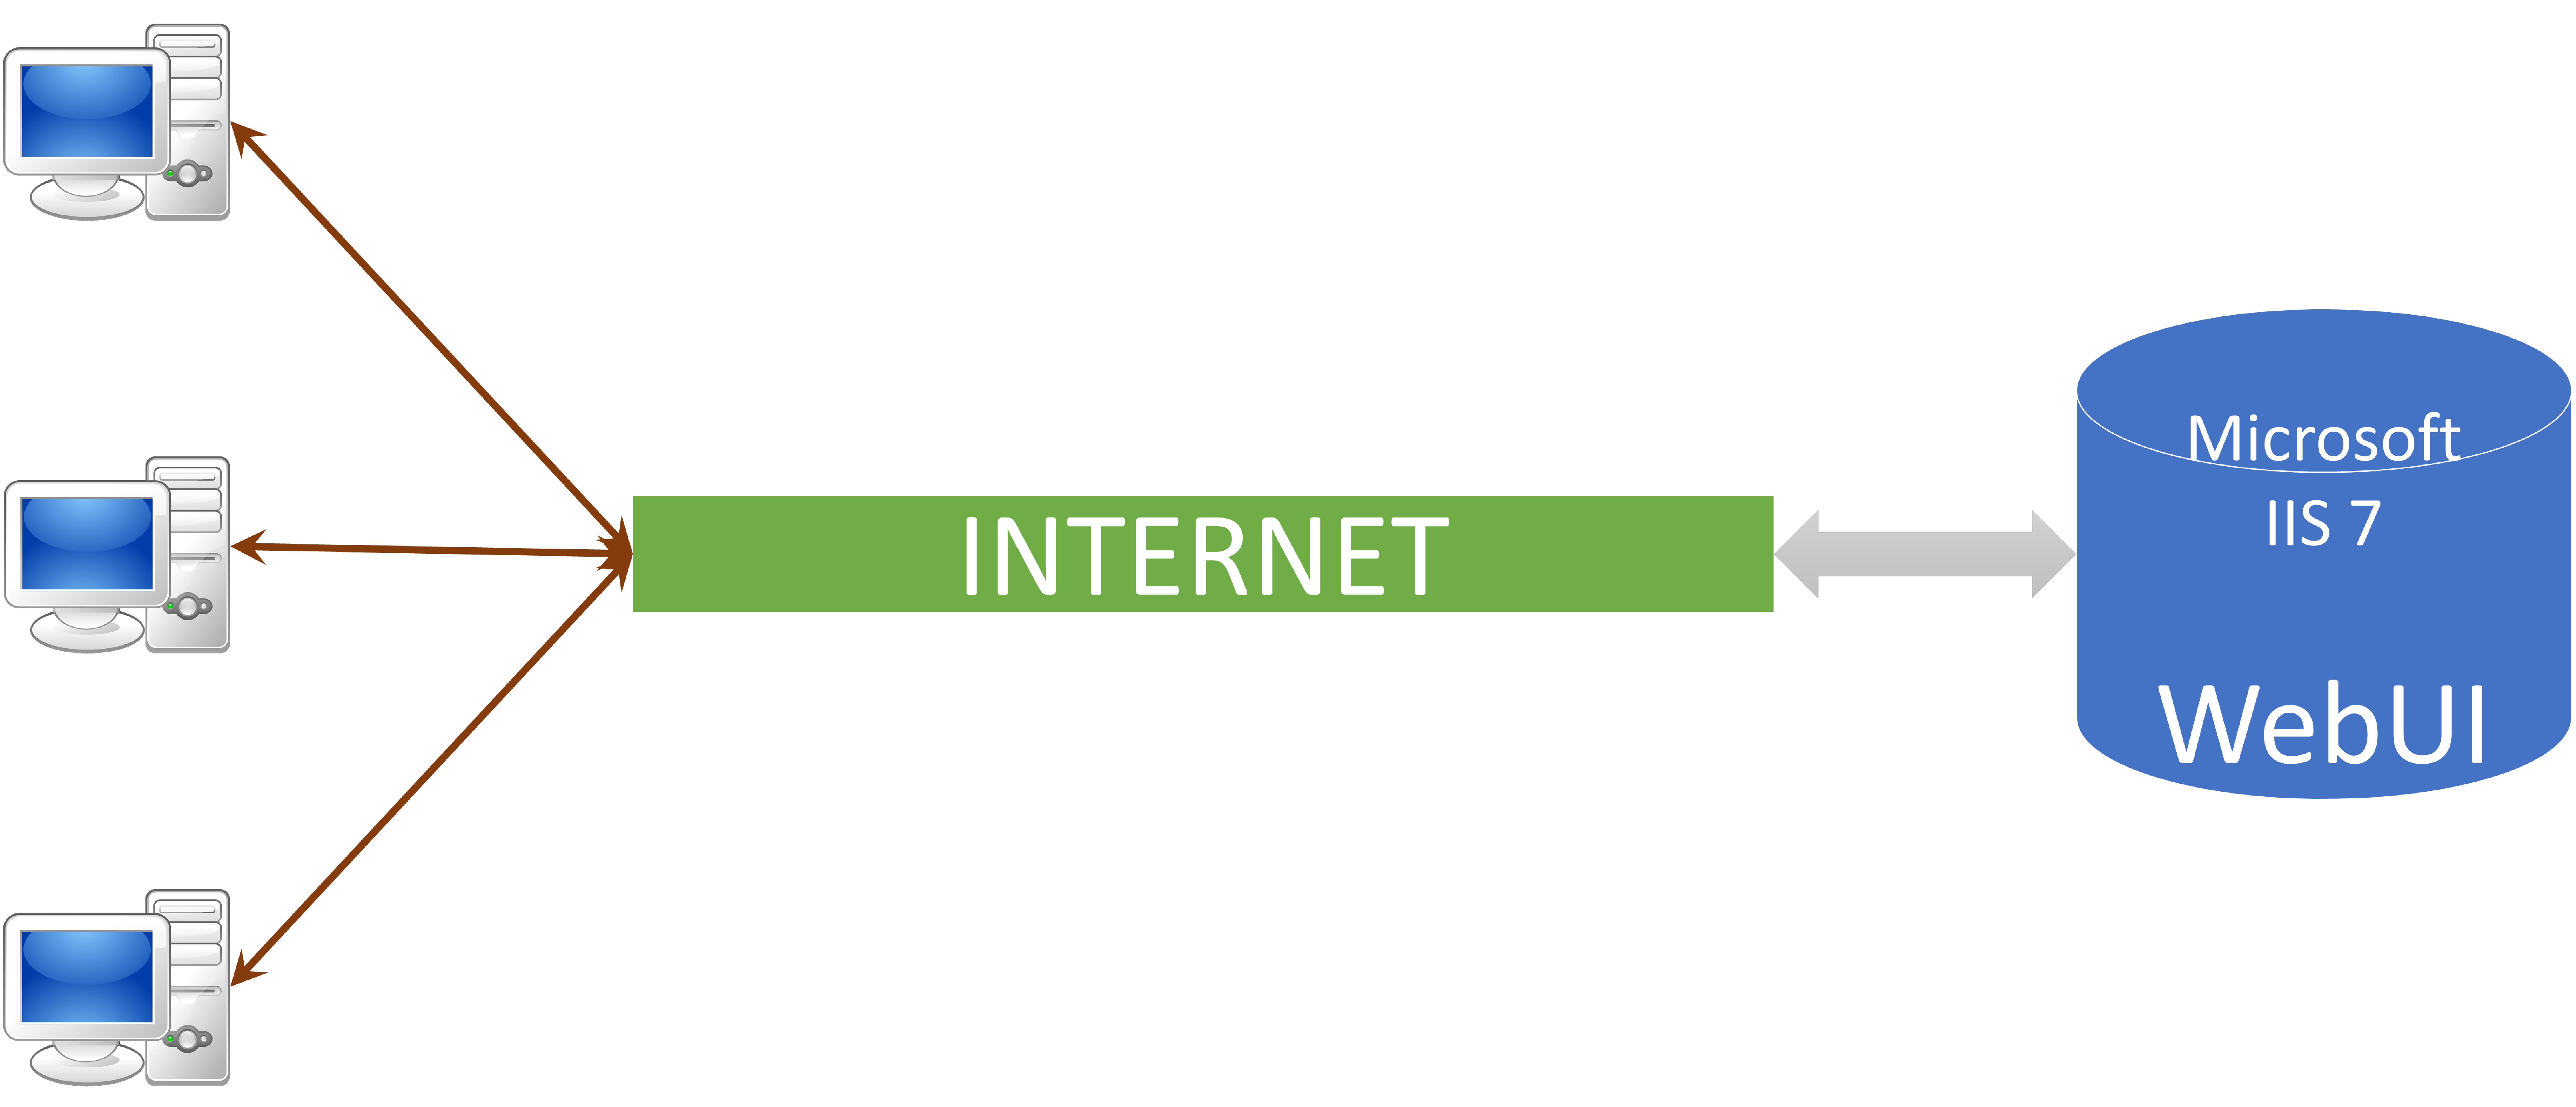
\includegraphics[width=1\linewidth]{Chapter3/chapter3/Fig9}
\caption[Framework behind WebUI for hardware G-FLCS]{Framework behind WebUI for hardware G-FLCS}
\label{fig:fig3_9}
\end{figure}
 
\subsection{WebUI for Hardware G-FLCS}
\begin{figure}
	\centering
	\subfloat[Basic Parameters]{\label{fig:BasicParameters}\includegraphics[scale=0.38]{Chapter3/chapter3/Fig3.eps}} \\
	\subfloat[Input Membership]{\label{fig:InputMembership}\includegraphics[scale=0.38]{Chapter3/chapter3/Fig4.eps}} 
	\caption{WebUI for Hardware G-FLCS developed using ASP.NET with C\# and hosted using Microsoft IIS7}
	\label{fig:WebUI}
\end{figure}
\begin{figure}
	\centering
%	\ContinuedFloat 
	\subfloat[Output Membership]{\label{fig:OutputMembership}\includegraphics[scale=0.38]{Chapter3/chapter3/Fig5.eps}} \\
	\subfloat[Rulebase]{\label{fig:RuleBase}\includegraphics[scale=0.38]{Chapter3/chapter3/Fig6.eps}} 
	\caption{WebUI for Hardware G-FLCS developed using ASP.NET with C\# and hosted using Microsoft IIS7}
	\label{fig:WebUI2}
\end{figure}
\par
WebUI is developed in ASP.NET with C\# and deployed using Microsoft IIS-7. The Web Pages that serves to collect various information pertaining to parameters related to FLC from users are shown in Figure \ref{fig:WebUI} and Figure \ref{fig:WebUI2}. Web page in Figure \ref{fig:BasicParameters} presents the WebUI where, parameters like \textit{name}, \textit{type}, \textit{implication}, \textit{aggregation}, \textit{and} method,\textit{ or} method and \textit{defuzzification} type are defined. Web page in Figure \ref{fig:InputMembership} accepts details of inputs and their MFs whereas Web page in Figure \ref{fig:OutputMembership} accepts details about outputs and their corresponding MFs. Web page in Figure \ref{fig:RuleBase} accepts the Rulebase and stores all data in FCP file as mentioned in Appendix. On submission, these information data are validated and a server application for communication with the board is invoked. This WebUI can be accessed over Ethernet from a client system situated far away from the controller and plant (simulated model).

\section{Genetic Algorithm based Fuzzy Parameter Extraction} \label{sec:FCP}
A genetic algorithm (GA) is a search heuristic that mimics the process of natural selection and has been widely used evolutionary method for optimization of FLCs, both type I and II\cite{Ishibuchi1995a,Shopova2006,Bandyopadhyay2001a,Maldonado2014,Alcala2006a,Sanz2011}. This technique has been widely used in the literature for fuzzy optimization. Other popular methods for fuzzy optimization are Univariate Marginal Distribution Algorithm (UMDA)\cite{bookBehera2009}, stochastic Hill Climbing(SHC) \cite{Michta2011,Chen2003a}, Baysian Optimization Algorithm (BOA) \cite{Jiang2000}. 
\begin{table}
	\centering
	\caption{Genetic Algorithm Parameters}
	\label{tab:GS_Param}
	\begin{tabular}{cc}
		\hline Parameters & Value/Function \\ 
		\hline Population & 120 \\ 
		Generation & 200 \\ 
		Fitness Scaling & Rank \\ 
		Selection & Stochastic \\ 
		Crossover Probability & 0.8 \\ 
		Elite Count & 6 \\ 
		Mutation Function & Adaptive feasible  \\ 
		Crossover Function & Adaptive feasible  \\ 
		Stopping Criteria & Fitness Limit \\ 
		\hline 
	\end{tabular} 
\end{table}

\begin{figure}[h!]
	\centering
	
\includegraphics[width=0.85\linewidth]{Chapter3/chapter3/Fig7_offline.eps}
	\caption{Fuzzy Control Parameter (FCP) extraction using Genetic Algorithm}
	\label{fig:fig3_7}
\end{figure}
Response from a system with maximum of four inputs and one output is recorded. Once the dataset is derived, it is passed on to the system for FCP extraction. The proposed method for FCP extraction is based on Genetic Algorithm. Details of the parameters used in Genetic Algorithm is displayed in Table \ref{tab:GS_Param}. There are 60 system parameters that are optimized using genetic algorithm to achieve two objectives, namely
\begin{itemize}
	\item Quick settling, and
	\item Tracking reference.
\end{itemize}
Figure \ref{fig:fig3_7} portrays basic blocks of a Genetic Algorithm based FCP extraction technique. An initial set of random parameters are input to the Genetic Algorithm system. Every optimization technique operates on a cost function. The cost function can be represented by the process plant simulation model or its I/O dataset. The FCP parameters are manipulated such that a set of optimized FCP is obtained which provide quick settling and fast reference tracking.  
The Simulink model with initial FCP is used as an objective function which returns the transient and settling time. The co-ordinates of the membership functions are treated as the nonlinear inequality constraints. Thus varying these FCP will provide with an absolute tracking of reference\footnote{The codes can be downloaded from \url{https://goo.gl/Zb17fZ}}.

\section{Data flow of the proposed system}
\begin{figure}[h!]
	\centering
	\includegraphics[width=1\linewidth]{Chapter3/chapter3/Fig8.eps}
	\caption{Dataflow of the proposed G-FLCS system}
	\label{fig:fig3_8}
\end{figure}
In this implementation process, data synchronization and communication between user and the hardware G-FLCS is critical. The process is presented in Figure \ref{fig:fig3_8}. This figure depicts how data communication is achieved with the help of various control signals between, client-server and server-GFLCS. The web application provides a systematic user interface which collects data from authenticated users. The application waits for a new connection request on startup. On successful login, the user is presented with a web page containing four different tab-windows, each for basic parameters, information about inputs, outputs and Rulebase. These windows are preloaded with extracted parameters as presented in Figure \ref{fig:fig3_7} and provide a way for fine tuning the control parameters by an operator. In Figure \ref{fig:fig3_8}, operations like connections, login, parameter collection and communication with hardware G-FLCS through a server program are performed by the web application and are shaded in \textit{Light Grey}. 
When a user provides the fuzzy control parameters (FCP) data, the web application validates the entered data based on following protocols.
\begin{itemize}
	\item All MFs have properly defined co-ordinates within specified range of operation.
	\item Number of Input(s) and Outputs are correctly defined. 
	\item Rules are validated according to Mamdani model.
\end{itemize}
After validation of new parameters, the server application connects serially to the hardware G-FLCS. Serial communication protocol has been used here for the ease of implementation. This data communication can be easily extended to industry standard controller area network (CAN) protocol. G-FLCS completes current execution and generates control signal to the system. Thereafter, it acknowledges any incoming serial communication request and starts receiving and storing fuzzy parameters in the data memory. Sys/BIOS is widely used real time operating system for TI DSPs and has been used in this work to take care of the multitasking of fuzzy processes.


\section{System Integrity Test}
To provide proof of concept for this proposed design, an experiment was carried out with an Intel Corei5-2400 3.1 GHz PC with 4GB memory operating as a server with the WebUI. It is available to all the clients in the local network over same gateway. Authenticated user loads FCP data in a text file located in the server. 

\begin{figure}[h!]
	\centering
	\subfloat[Plant Output: Two Tank Water Level System]{\label{fig:TT_Out}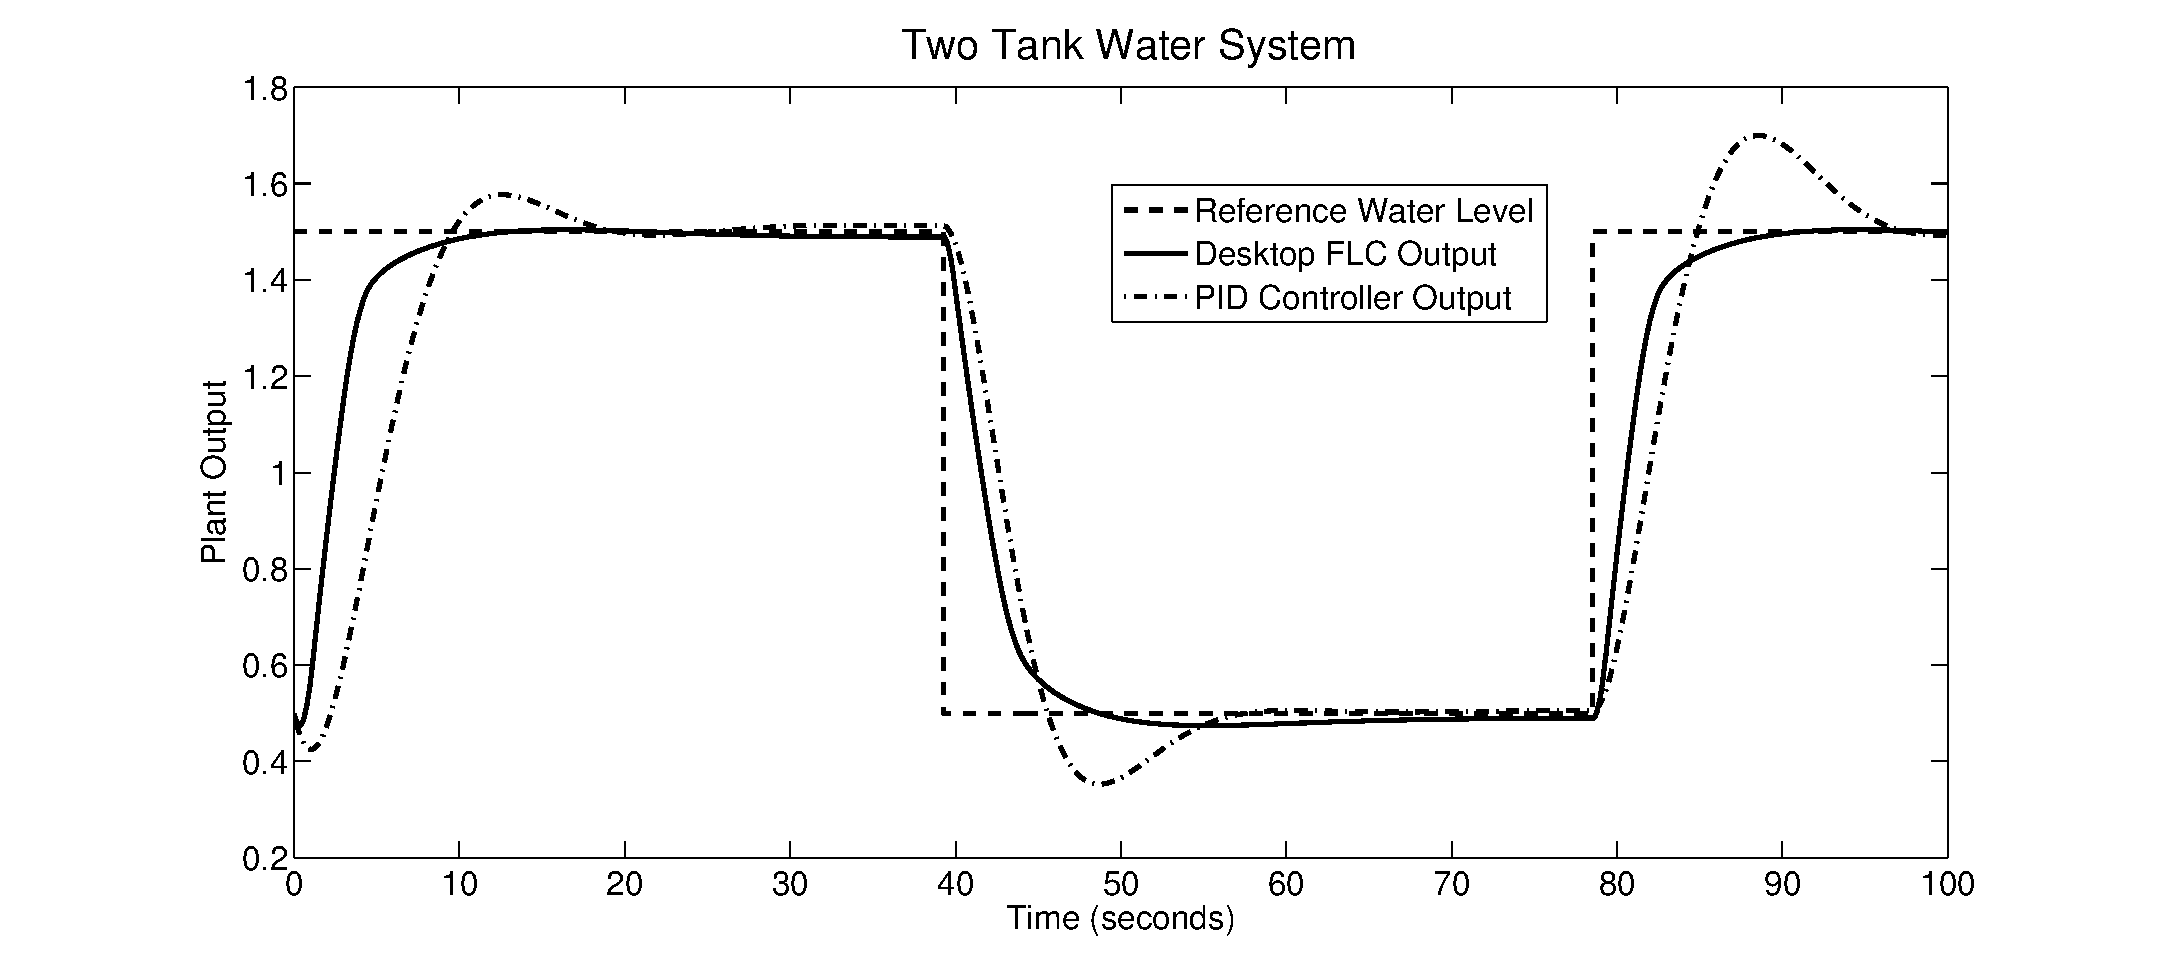
\includegraphics[width=0.9\linewidth]{Chapter3/chapter3/TankPO.eps}} \qquad
	\subfloat[Controller Output: Two Tank Water Level System]{\label{fig:TT_Con}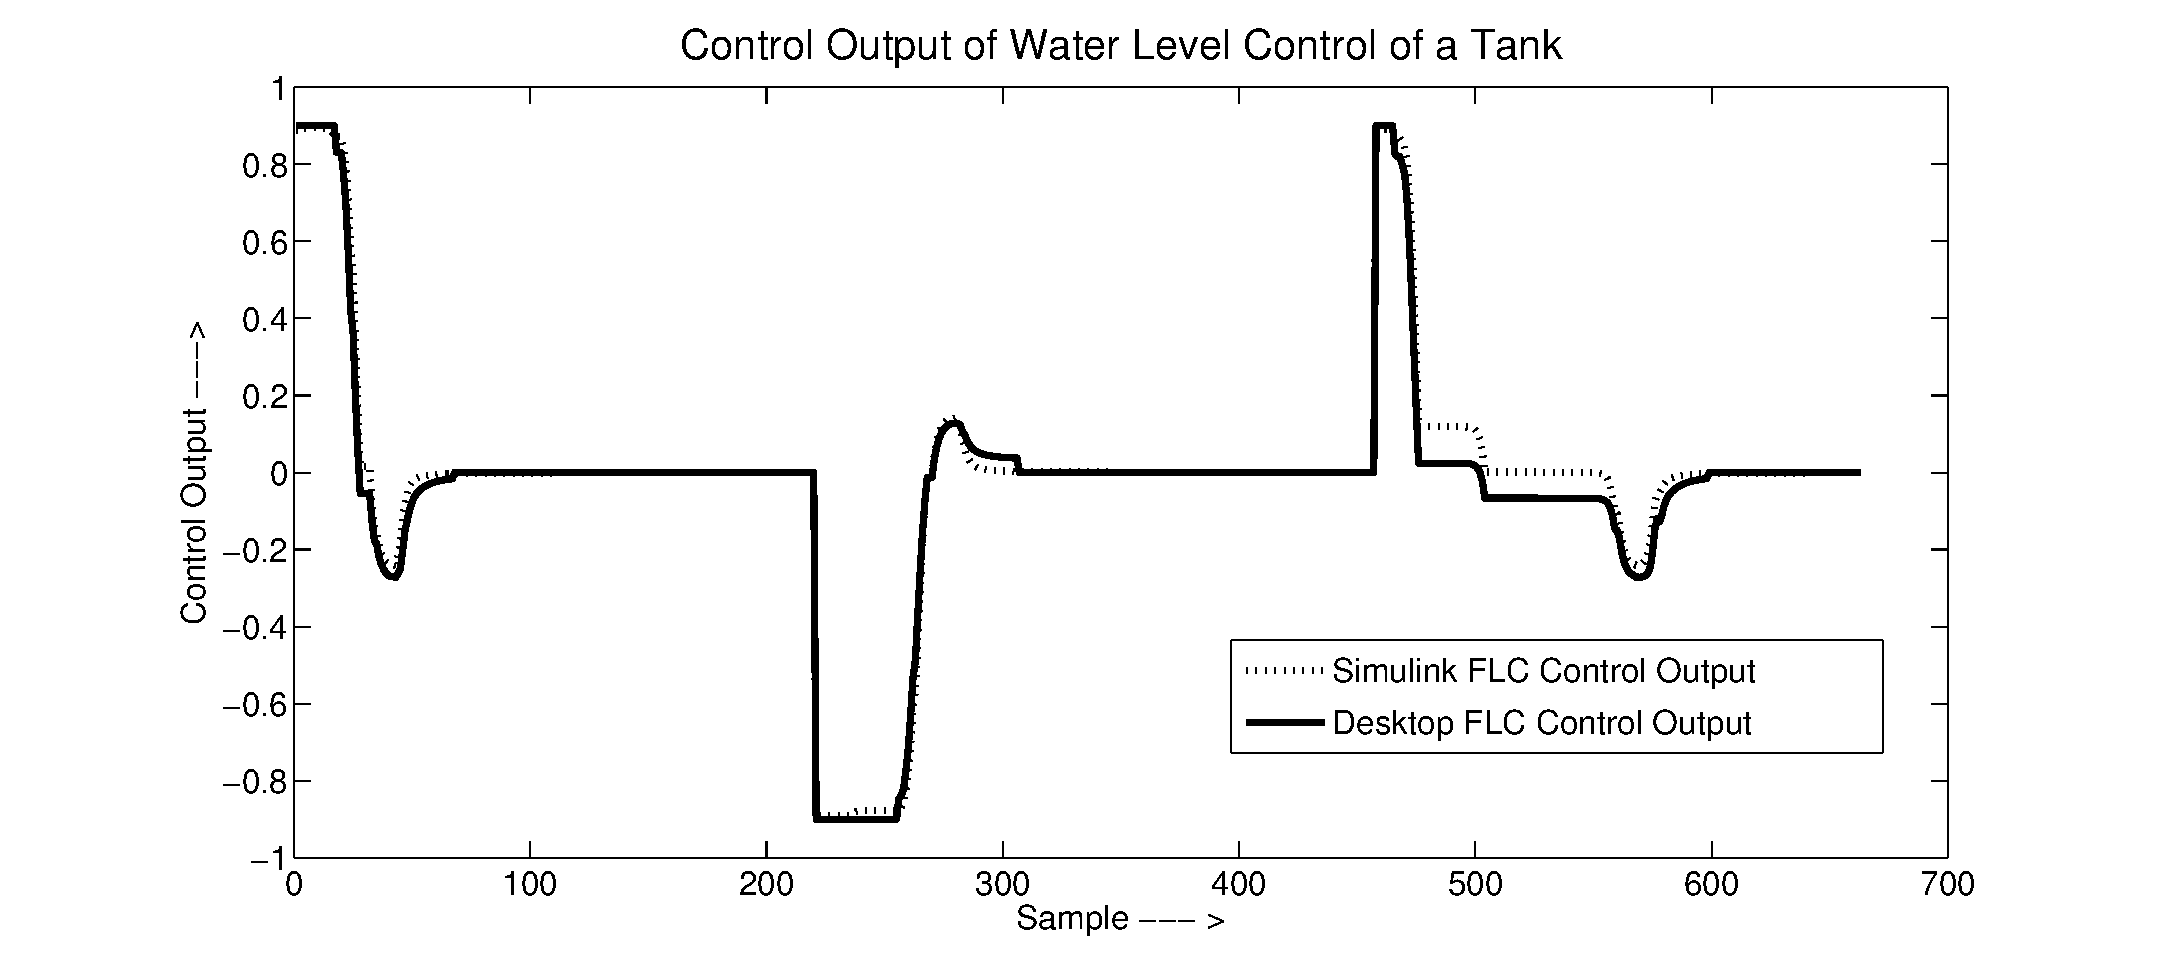
\includegraphics[width=0.9\linewidth]{Chapter3/chapter3/TankCO.eps}}
	\caption{Plant output and Controller output of various test models. The controller output is a comparison between output from Matlab Fuzzy Logic Toolbox and proposed hardware G-FLCS. Plant output shows performance of the proposed FLC structure with PID controllers conducted using through HIL testing environment} 
	\label{fig:CompOut_tank}
\end{figure}

\begin{figure}[h!]
	\centering
	\subfloat[Plant Output: Intelligent Cruise Control System]{\label{fig:ICC_Out}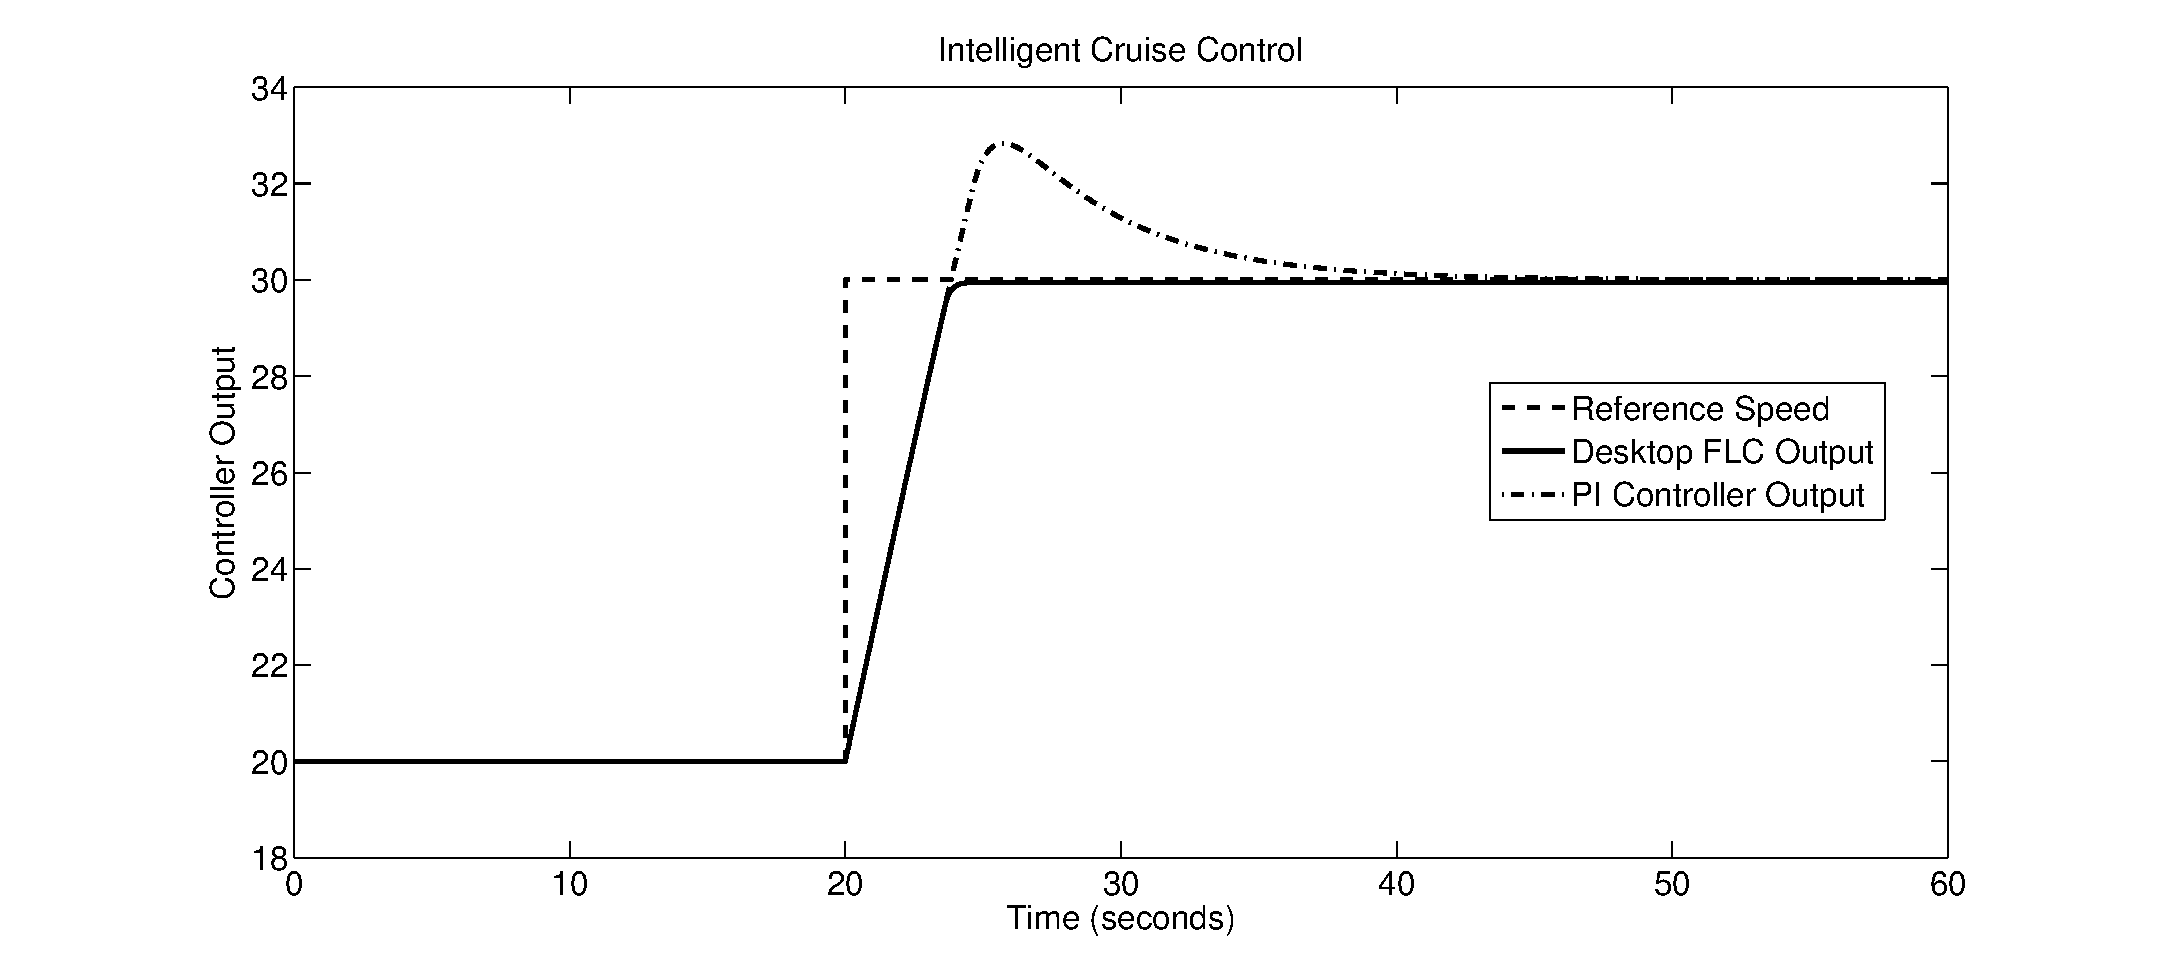
\includegraphics[width=0.9\linewidth]{Chapter3/chapter3/IccPO.eps}}\\
	\subfloat[Controller Output: Intelligent Cruise Control System]{\label{fig:ICC_Con}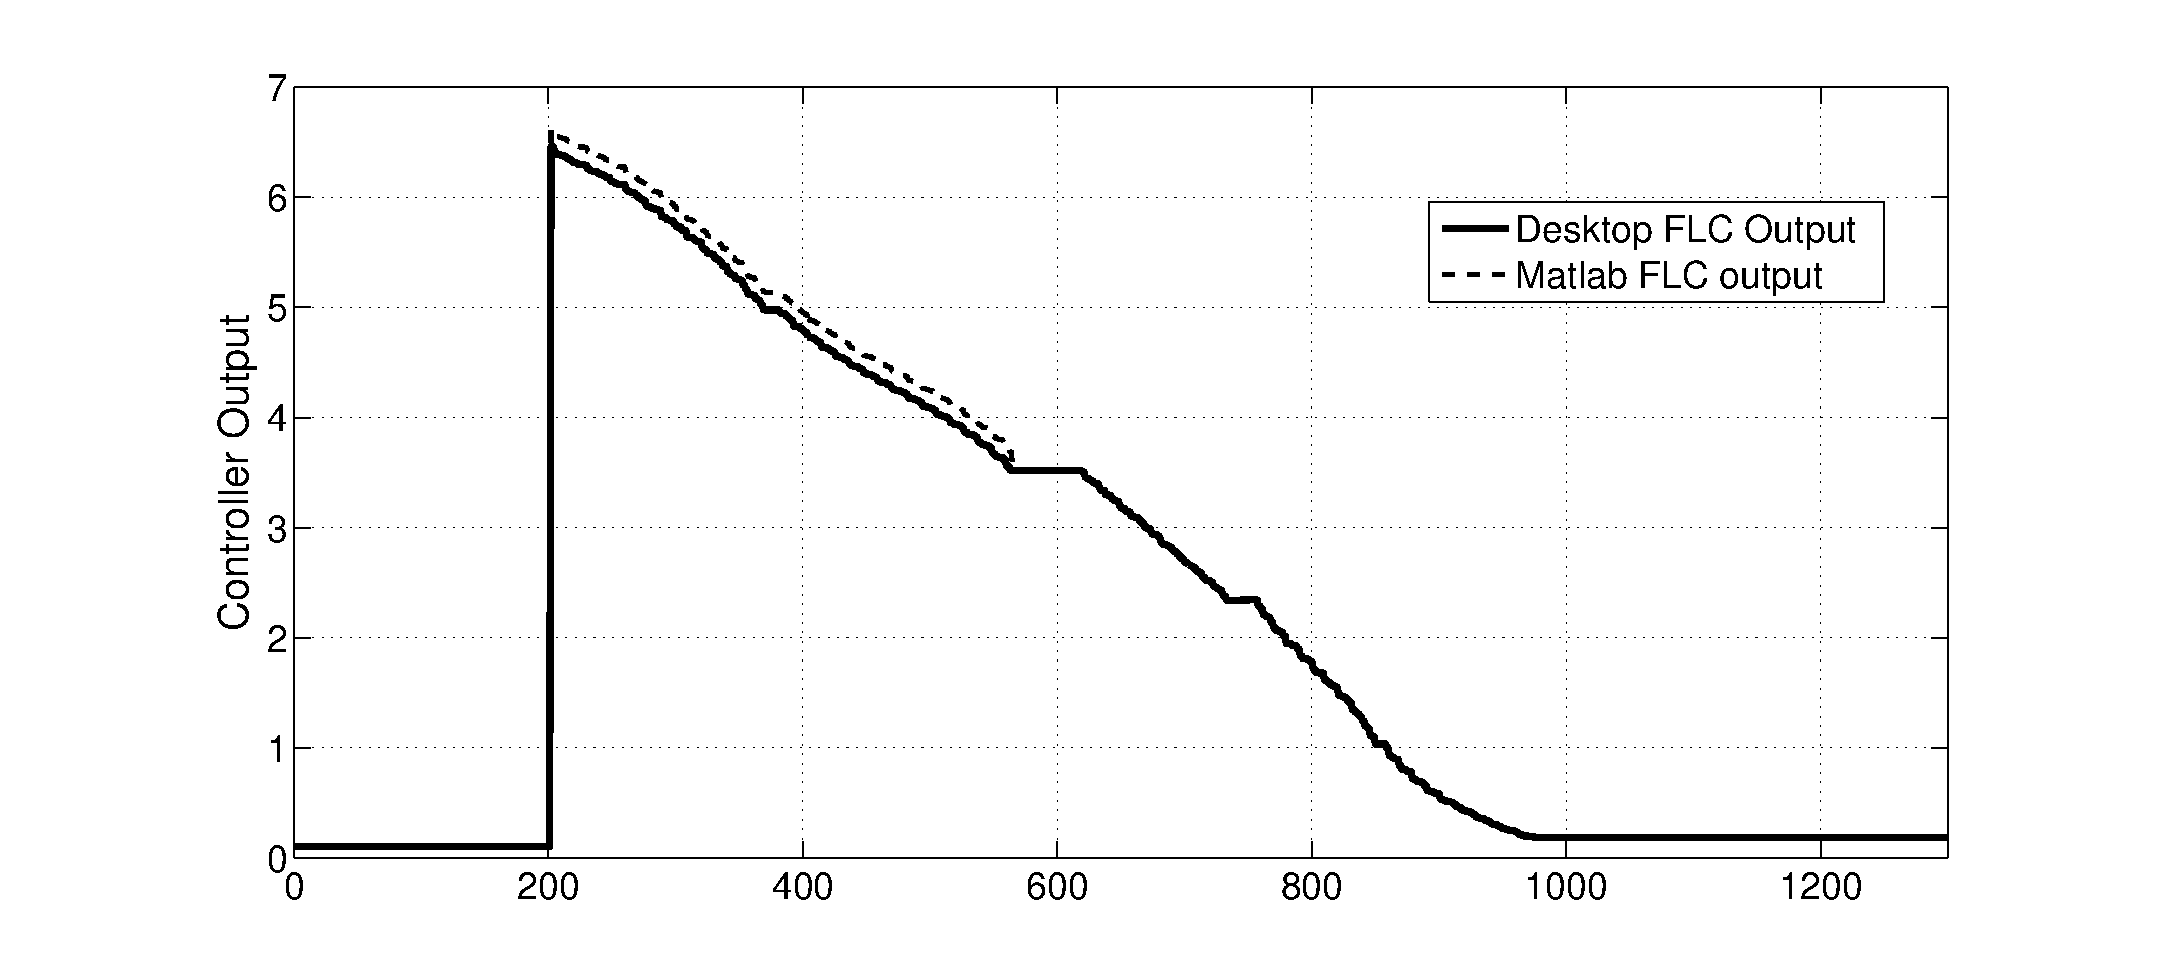
\includegraphics[width=0.9\linewidth]{Chapter3/chapter3/IccCO.eps}}
	\caption{Plant output and Controller output of various test models. The controller output is a comparison between output from Matlab Fuzzy Logic Toolbox and proposed hardware G-FLCS. Plant output shows performance of the proposed FLC structure with PID controllers conducted using through HIL testing environment} 
	\label{fig:CompOut_icc}
\end{figure}


\begin{figure}[h!]
	\centering
	\subfloat[Plant Output: First-order system with dead time for anti-windup scheme]{\label{fig:AWU_Out}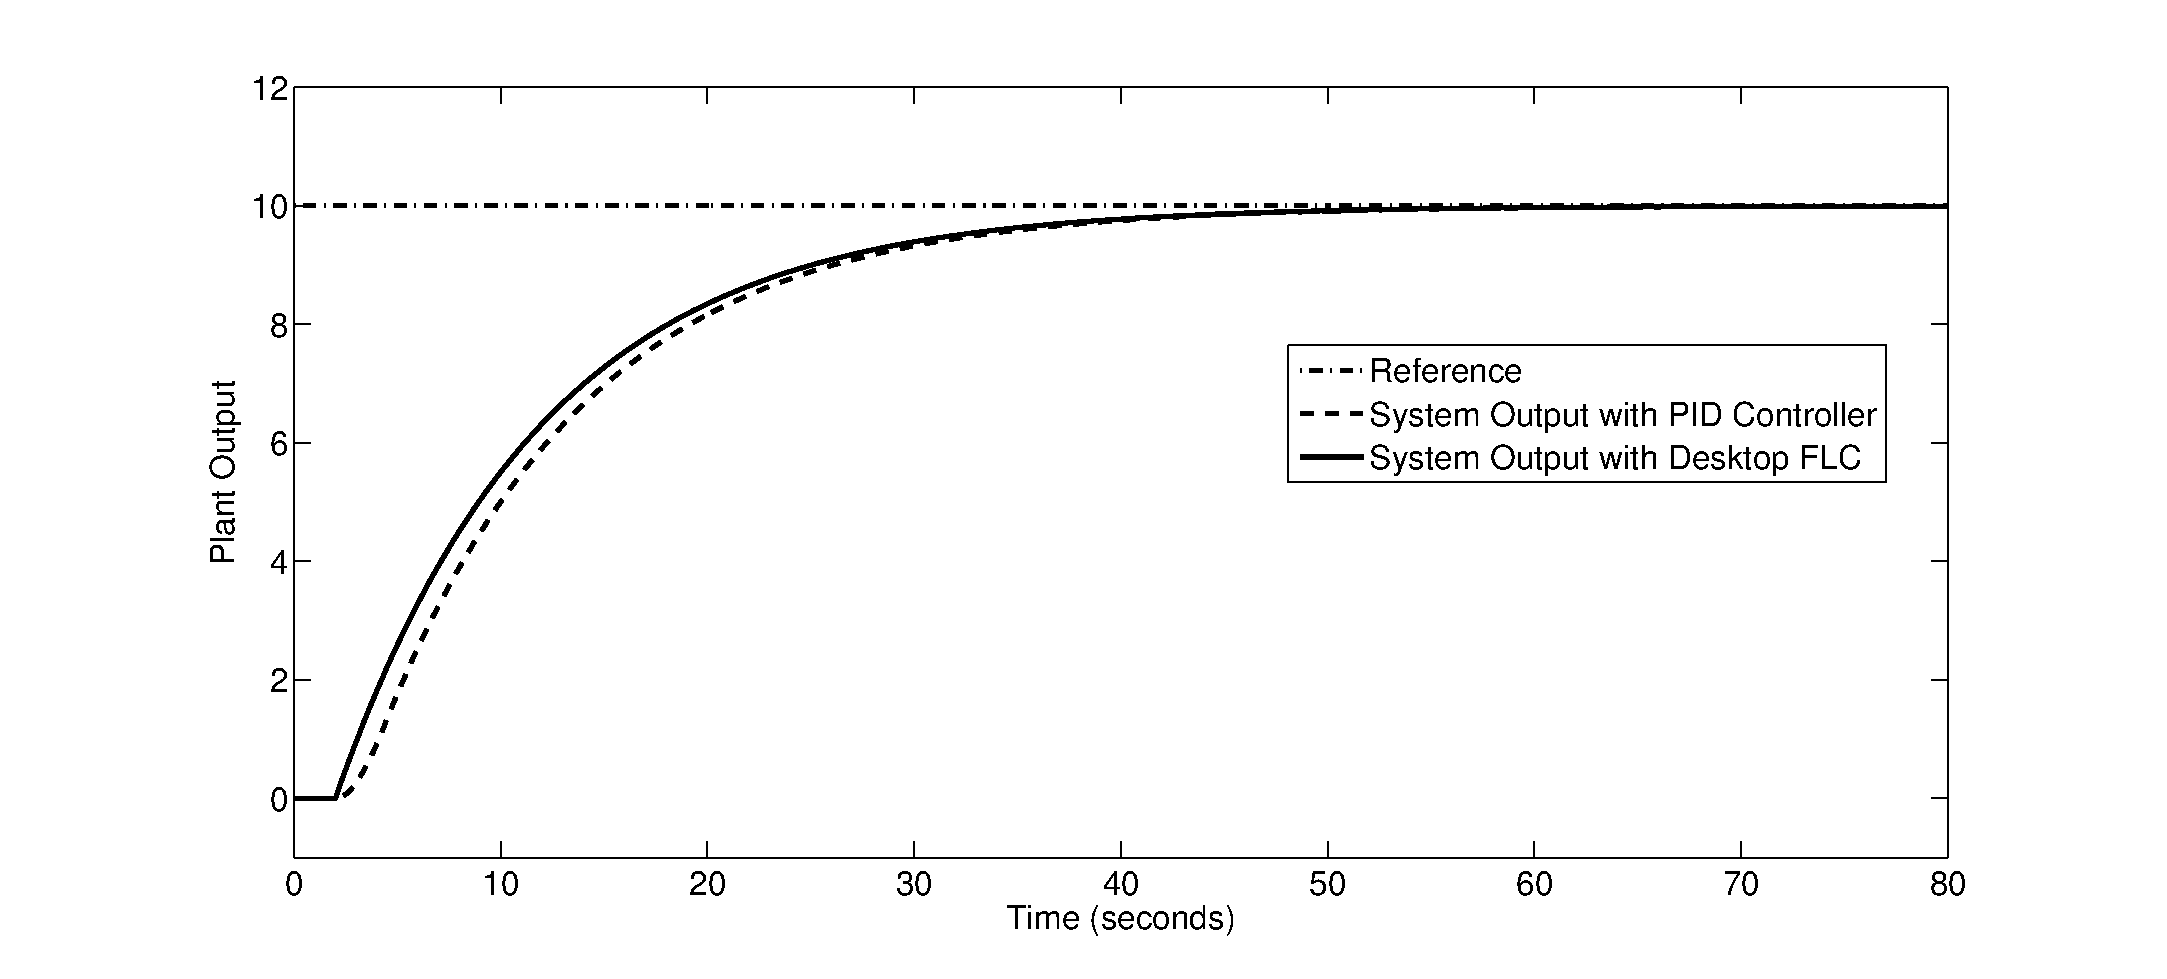
\includegraphics[width=0.9\linewidth]{Chapter3/chapter3/AwbPO.eps}} \qquad 
	\subfloat[Controller Output: First-order system with dead time for anti-windup scheme]{\label{fig:AWU_Con}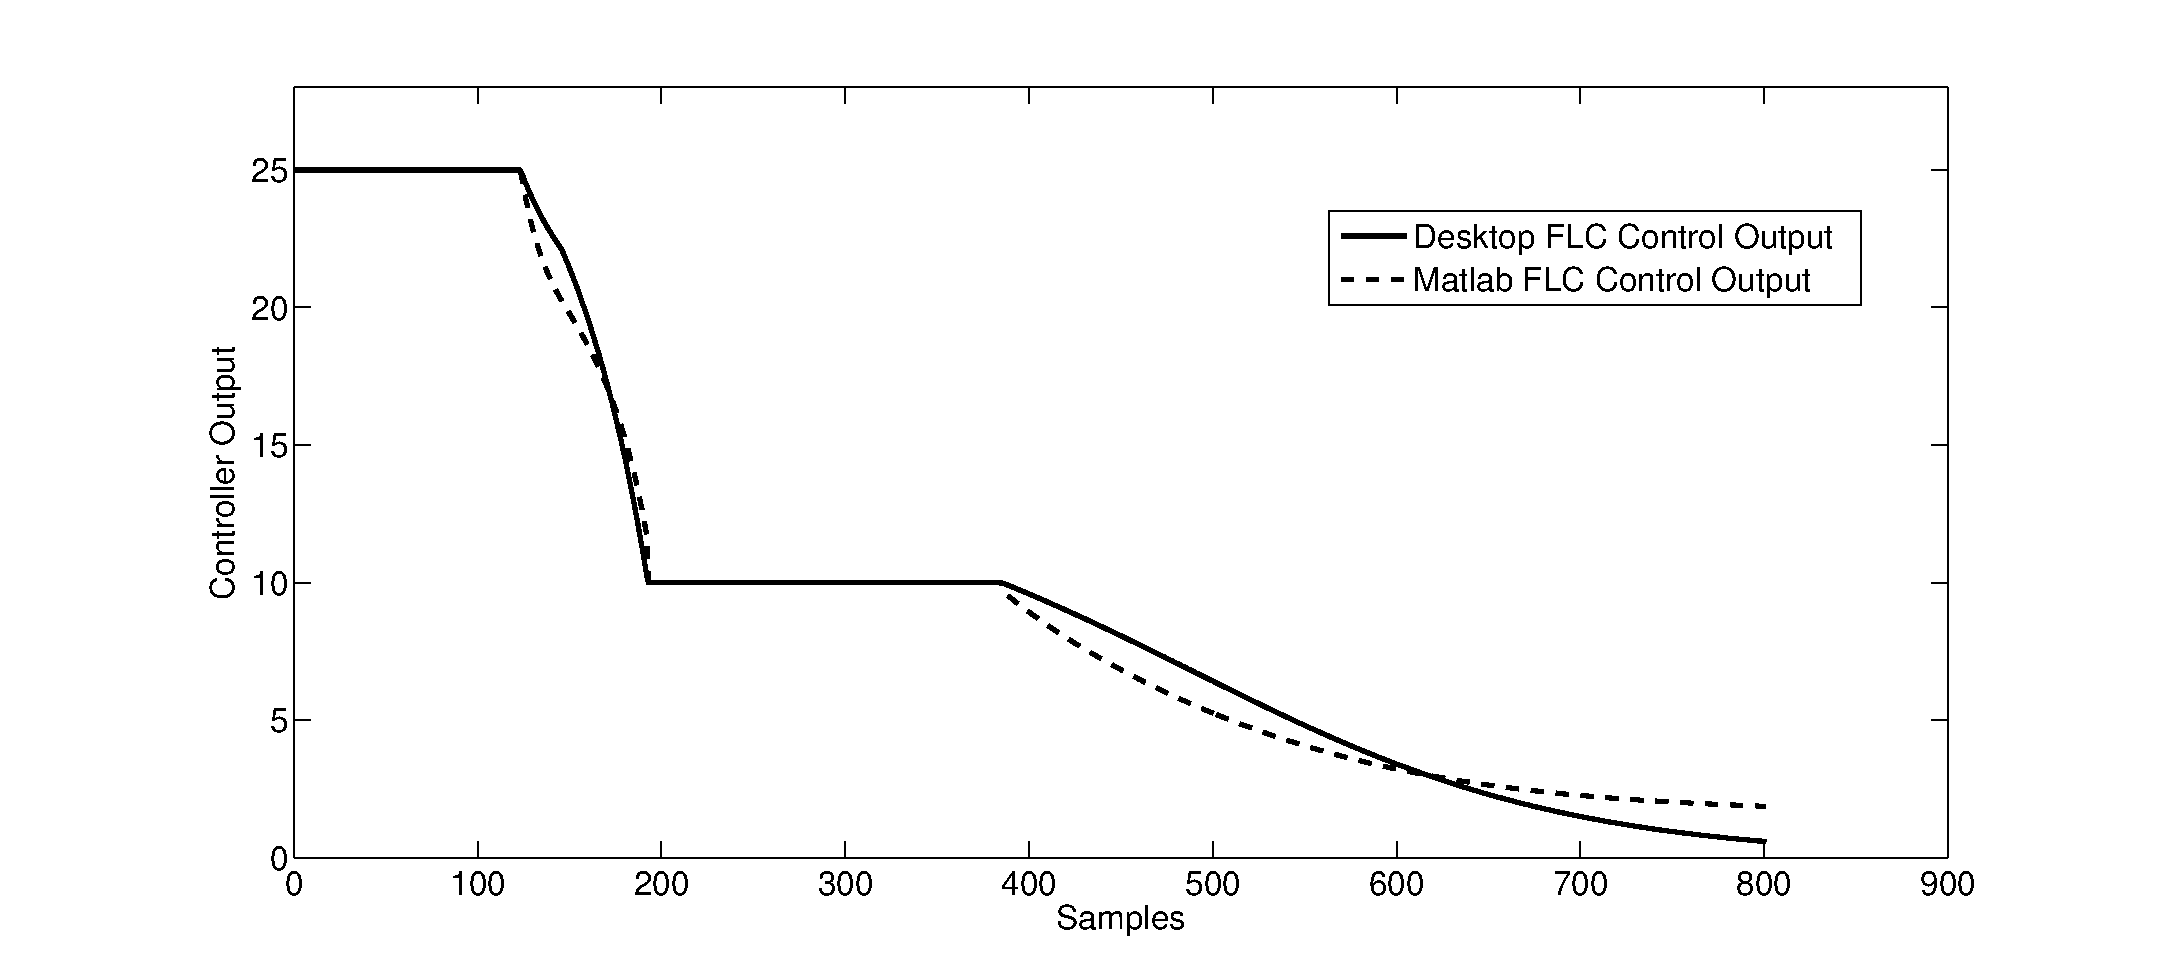
\includegraphics[width=0.9\linewidth]{Chapter3/chapter3/AwbCO.eps}}
	\caption{Plant output and Controller output of various test models. The controller output is a comparison between output from Matlab Fuzzy Logic Toolbox and proposed hardware G-FLCS. Plant output shows performance of the proposed G-FLCS structure with PID controllers conducted through HIL test environment} 
	\label{fig:CompOut_wind}
\end{figure}

The code developed for hardware G-FLCS is compiled using MS Visual Studio to generate a desktop application which runs on the server and mimics the hardware G-FLCS. This FCP data is used by desktop FLC to generate control signal. Plant models are developed in Matlab and communicates with the desktop FLC using $ system $ command. The functionality is executed in following steps:
\begin{description}\label{algo:StepsSim}
	\item[Step 1] Generation of I/O dataset from Simulink model using PID controller.
	\item[Step 2] Apply GA based FCP extraction algorithm described in section \ref{sec:FCP}, to extracted FCP from the I/O dataset generated in Step 1. 
	\item[Step 3] Appropriate FCP data is programmed through WebUI and submitted to the server.
	\item[Step 4] The plant model is executed with the stored FCP. For controlling the plant, Matlab uses $ system $ command to invoke the desktop FLC program and passes the FCP and input data \_IN as arguments. Desktop FLC computes and returns the output to Matlab. This forms the controller output.
	\item[Step 5] The Simulink plant output is computed with controller output. It is stored and plotted with respect to plant output using PID controllers for comparative analysis.
	\item[Step 6] The dataset is used to compare the control signal from desktop FLC to control signal from Matlab Fuzzy Inference System for performance analysis.
\end{description}
 
Some benchmark control problems were used to test the applicability and generality of the proposed architecture, namely Two Tank Water Level Controller \cite{twotank2012,Laubwald2006}, Intelligent Cruise Control \cite{Naranjo2003}, first order system with dead time for anti-windup scheme \cite{antiwindup2014}. All these system models were implemented on Simulink and they are available in Mathworks File Exchange repository. The integrity of the proposed architecture is tested with these models according to the algorithm described above. In Figure \ref{fig:CompOut_tank}, Figure \ref{fig:CompOut_icc} and Figure \ref{fig:CompOut_wind} the observed results from these simulated tests are displayed. The proposed MT-FRHC based Web Configurable G-FLCS is implemented on the desktop server using C code interface by an application program to the WebUI. This provides a platform for evaluation of the proposed technique before it is realized on actual hardware platform. In Figure \ref{fig:TT_Out}, the plant output of this proposed desktop G-FLCS is compared to a tuned PID controller when applied to control a Two Tank Water Level Controller \cite{twotank2012,Laubwald2006}. The figure plots the plant response under different controllers with respect to time in seconds. It can be observed that the proposed G-FLCS provides a smooth and fast control compared to the PID controller. Similar results are observed when the proposed GFLCS and a tuned PID controller is employed to control an Intelligent Cruise Control System\cite{Naranjo2003} and first order system with dead time for anti-windup scheme \cite{antiwindup2014}. These figures plots the plant response under desktop G-FLCS and PID controller with respect to time in seconds. Figure \ref{fig:ICC_Out} and \ref{fig:AWU_Out} shows that the G-FLCS performs better than the PID controller. Figure \ref{fig:TT_Con}, Figure \ref{fig:ICC_Con} and Figure \ref{fig:AWU_Con} compares the control output from the desktop G-FLCS and Matlab FLT for every sample while controlling Two Tank Water Level Controller \cite{twotank2012,Laubwald2006}, Intelligent Cruise Control \cite{Naranjo2003} and first order system with dead time for anti-windup scheme \cite{antiwindup2014} process plants respectively. These tests indicates that the objective of generality and remote reconfigurability is achieved for proposed MT-FRHC based G-FLCS design. The results also convincingly reflects that the proposed system architecture performs satisfactorily and can be implemented on real-time. However, its real-time nature can be concluded only after conducting the timing analysis and profile. This is presented in the next chapter along with the aspects of hardware implementation.

\section{Summary}
This chapter presents a background framework for MT-FRHC based remotely tunable G-FLCS. The proposed controller can suitably replace existing controllers in a process plant which confirms the generic nature of the designed G-FLCS. The algorithm for achieving this is described in section \ref{sec:FCP}. In this work, process control applications based on PID controller were chosen specifically. The major reason is their wide usage and acceptability in industries. By following protocols mentioned in section \ref{sec:FCP}, other variants of industrial controllers like sliding mode and model predictive controllers can also be suitable approximated by the proposed G-FLCS. This chapter elaborates the proposed MT-FRHC based remotely tunable G-FLCS architecture with Genetic Algorithm based FCP extraction technique. The generality and applicability of the design is also tested by applying it to various benchmark control problems in a simulation environment. The results portrays a proof-of-concept for the objectives that were set in chapter 1. However, the major aspect of its implementation is yet to be evaluated. The next chapter deals with the prospect of implementation of the proposed G-FLCS and explain various schemes adopted to make the design feasible on a DSP platform.  




\chapter{Implementation of Remotely Tunable MT-FRHC based G-FLCS with VBCoA on Programmable DSP}

\begin{chapterAbstract}{Preview}
	This chapter present a MT-FRHC based remotely tunable G\hyp{}FLC implemented on a programmable DSP platform. The algorithm is ported on a single core fixed point DSP, which can be remotely configured in real\hyp{}time over Ethernet. This feature of reconfigurability enables a user to change fuzzy parameters in real\hyp{}time, eliminating repeated hardware programming. The scheme also eliminates the requirement of removing the controller from the process plant for configuration. A hardware software co\hyp{}design architecture for the proposed generic FLC is developed on TI C6748 DSP with Sys/BIOS RTOS and seamlessly integrated with a web based user interface (WebUI) for reconfigurability. The WebUI acquires the fuzzy parameters from users and a server application is dedicated to data communication between the hardware and the server. Analysis of this design is carried out by using hardware\hyp{}in\hyp{}loop (HIL) test to control various plant models in Simulink/Matlab environment. Performance of the proposed system is compared to Fuzzy Toolbox of Matlab and PID controllers.
\end{chapterAbstract}
\clearpage

\section{Introduction}
In previous chapter, the proposed MT-FRHC based remotely tunable G-FLCS architecture with Genetic Algorithm based FCP extraction technique is described. The results convincingly depicted that the objectives set in chapter 1 can be achieved in simulation environment. This chapter extrapolates the concepts introduced in last chapter to implementation it on a DSP platform. This chapter also introduces implementation and optimization of the code to realize the proposed MT-FRHC based G-FLCS with VBCoA defuzzification method. It is important that the code size is reduced to its maximum for reliable operation of the system. Large code size decreases power efficiency and computational speed. Smaller code size require less memory fetching since larger part of the on chip memory will be available for execution. This also increases the stack size. In this implementation it is imperative that the code size is limited to 60\% of the on-chip SHRAM.

\section{Hardware Device: TI LCDK C6748}
To achieve an efficient implementation, it is important to understand the architecture of th hardware device before final implementation. With a sequential processing on a DSP device, the objective of the proposed MT-FRHC based G-FLCS with VBCoA defuzzification to meet 11K FLIPS achieved by Yi Fu et. al. \cite{Fu2010} for their G-FLCS architecture on an FPGA is unachievable. Hereby, the implementation of the proposed G-FLCS architecture has to be parallelized. With this context, the hardware device at hand, TI's LCDK C6478 needs to be inspected.

LCDK C6478 incorporates a TMS320C6748 DSP which is a floating point very long instruction word (VLIW) DSP processor running at 476 MHz clock frequency. This device supports SIMD (single instruction, multiple data)and double precision VLIW operations \cite{TexasInstruments2013}. It is reported that this is one of the speediest single precision device. This is an important feature of this device that suits the proposed G-FLCS architecture since all operations are single precision. SIMD instructions supports data parallelism as opposed to VLIW's instruction parallelism. To take leverage of the SIMD or VLIW operations, it is imperative that the typical architecture of the G-FLCS is reconsidered to match either of these features of the device considering the functional block diagram in \ref{fig:functional_block}. 

\begin{figure}[h]
\centering
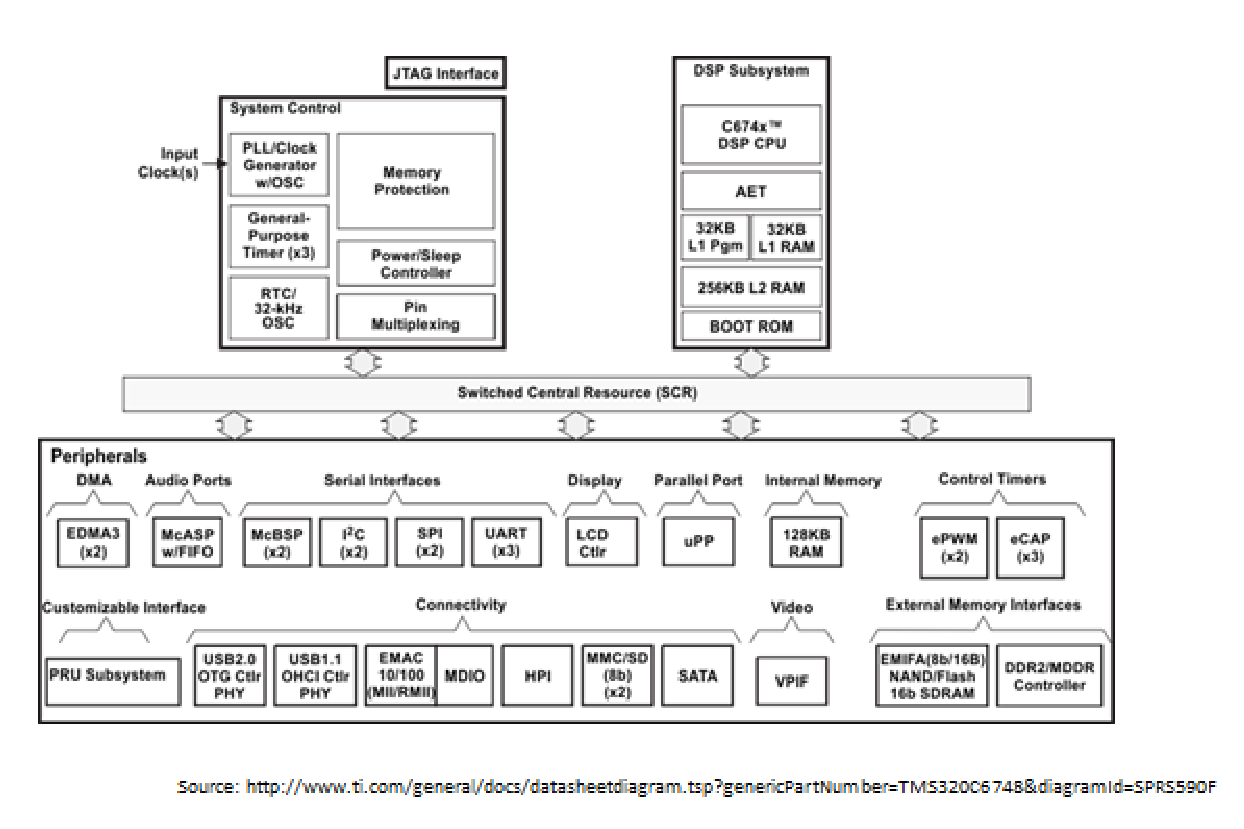
\includegraphics[width=0.9\linewidth]{Chapter4/chapter4/functional_block}
\caption{Functional Block Diagram of TMS320C6748 DSP}
\label{fig:functional_block}
\end{figure}

\section{Generic FLC on DSP (TI LCDK C6748)}
\subsection{System Architecture}
The system architecture of the proposed MT-FRHC based G-FLCS is represented as shown in \eqref{eq:MFRHC-final},
\begin{equation} 
{\theta _f}({c_j}) = \bigcap\limits_{{k_x} = 0}^{n_{op} - 1} {\left( {{\theta _f}\left( {{R_b}\left( {{k_x}} \right)} \right),\left( {\bigcup\limits_{l = 0}^{N - 1} {\overrightarrow {{C_{{R_v}}}\left( l \right)} } } \right)} \right)} 
\end{equation}
There are two data loops in this architecture. The inner loop is set to a small constant by the number of active MFs (in this case completely controlled by the user); while the outer loops are independent of the data. Therefore it can be concluded that the dependency of the outer loop is already parallelized in this architecture.

\subsection{Code Optimization} \label{sec:subsec1}
Generally a code that is written in assembly (ASM) is processor\hyp{}specific, whereas C code can readily be ported from one platform to another. However, optimized ASM code runs faster than C and requires less memory space. Before optimizing a code, it is required to make sure that the code is functional and yields correct results. After optimizing, the code can be reorganized and resequenced. The code becomes extremely difficult to follow and debug. It needs to be realized that if a C\hyp{}coded algorithm is functional and its execution speed is satisfactory, there may not be a necessity to optimize it further. All these motivates us to stretch the optimization so that the best possible efficiency is extracted from the system \cite{TexasInstruments2014,Batten2000}.
A rigorous code optimization strategy was devised as follows\cite{bookchassaing2005}:
\begin{description}
	\item[Step 1] G\hyp{}FLC is programmed in C Language without using any compiler optimization levels. With help of CCS Profiler tool, all the submodules are inspected for performance with respect to execution time and memory consumed.
	\item[Step 2] Intrinsic functions are used along with various compiler optimization levels. Functions like minimum (min), maximum (max), product (prod), division (div) are written as intrinsic functions and called as necessary by the modules and submodules of hardware G\hyp{}FLCS.
	\item[Step 3] Thereafter, the CCS Profiler tool is exploited again to determine and identify the functions and submodules that may need further optimization. 
	\item[Step 4] The functions that do not meet expected time and memory budget, are converted to linear ASM. The resultant is again inspected using the CCS Profiler tool to check for final efficiency.
\end{description}

 These process is realized in the system as follows: 
 \begin{enumerate}
 	\item `-o3' with optimization `-mt' 
 	\item `-k' with optimization `-mw' as feedback option for compiler
 	\item Minimize the loop carried dependency bound. 
 	\item MUST\_ITERATE and UNROLL pragmas.
 	\item Operate on single precision data type
 	\item SIMD
 	\item Intrinsics from TI library.
 \end{enumerate}

 \begin{table}[h]
 	\centering
 	\caption{Options in Compiler Level Optimization}
 	\label{tab:opti_param}
 	\resizebox{0.85\textwidth}{!}{%
 		\begin{tabular}{cc}
 			\hline
 			Options & Features \\ \hline
 			-o3 & \begin{tabular}[c]{@{}c@{}}This activates Compiler optimization level 3. \\ In this setting, the compiler majorly tries to \\ perform software pipelining.It also converts \\ small functions to inline calls.\end{tabular} \\ \hline
 			-mt & \begin{tabular}[c]{@{}c@{}}It explicitly mentions that the pointer-based \\ parameters of a function will never point to \\ the same location.\end{tabular} \\ \hline
 			-k, -mw & \begin{tabular}[c]{@{}c@{}}These options instruct the compiler to \\ generate feedback which can be analyzed \\ for tuning performance.\end{tabular} \\ \hline
 		\end{tabular}%
 	}
\end{table}

The compiler can insert calls to special functions in the run\hyp{}time support library (RTS) to support operations that are not natively supported by the ISA. For example, the compiler calls $\_\_c6xabi\_divi() $ ($ \_divi() $ in COFF) function to perform 32\hyp{}bit integer divide operation. Such functions are called compiler helper functions, and result in a function call within the loop body. For example in G\hyp{}FLC, the compiler accomplishes the division operation by calling the compiler helper function "$ \_divi $" in fuzzification and defuzzification modules.

\subsection{Code Implementation}
\begin{figure}[h!]
	\centering
	\subfloat[Without Optimization]{\label{fig:fig4_1}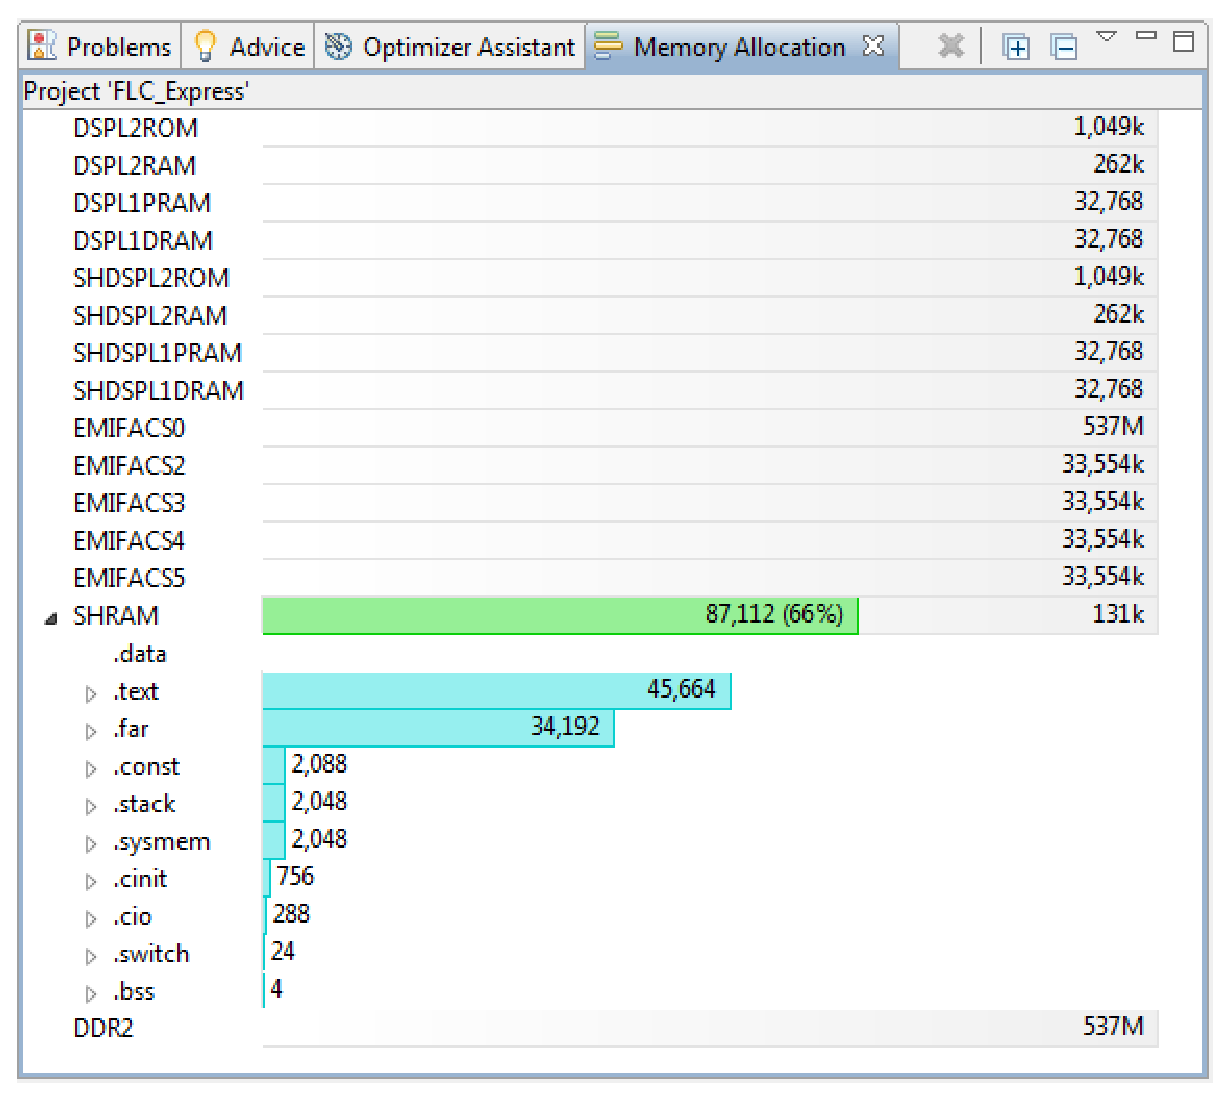
\includegraphics[width=0.95\linewidth,height=0.4\textheight]{Chapter4/chapter4/Fig1_MU}} \\
	\subfloat[Optimization]{\label{fig:fig4_2}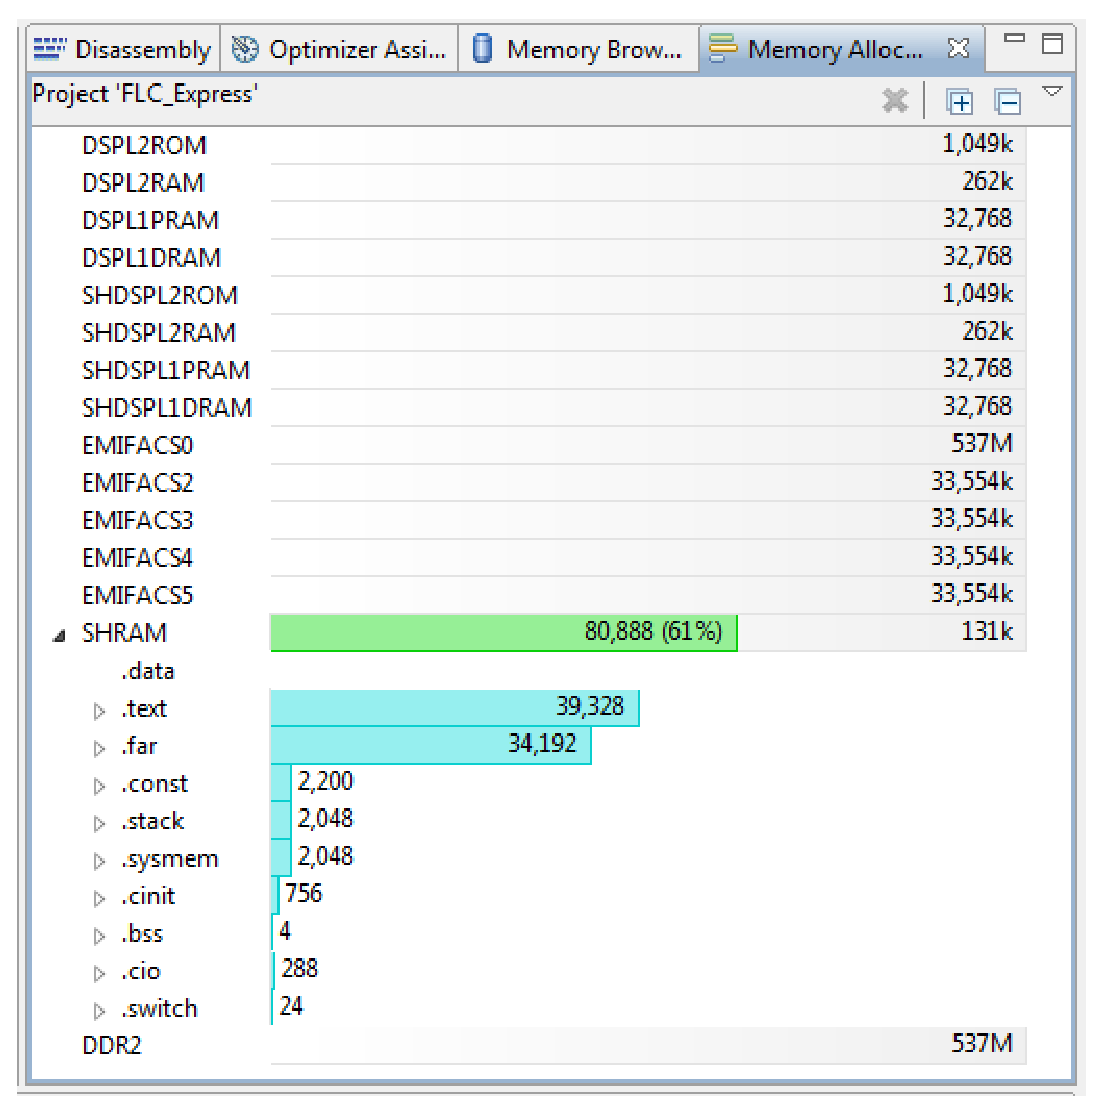
\includegraphics[width=0.95\linewidth,height=0.4\textheight]{Chapter4/chapter4/Fig2_MU_Opti}} 
	\caption{Memory Utilization of Proposed System Realized on TI C6748 DSP}
	\label{fig:Mem_Util}
\end{figure}
Code Composer Studio (CCS) is a proprietary integrated development environment developed by TI for programming DSP and ARM processors. The design is programmed in C language and optimized as described in section \ref{sec:subsec1}. Thereafter it is cross compiled using CCS v5.5 compiler and implemented on TMS320C6748 as target DSP processor. This system represents the hardware G\hyp{}FLCS as discussed previously. G\hyp{}FLCS is connected to a server PC using on\hyp{}board UART and provides a platform which is capable of accepting FCP file to operate as a standalone tunable G\hyp{}FLCS.

To achieve a high performance in throughput, the following optimization technique were used inside the developed code \cite{TexasInstruments2013}.
\begin{description}
	\item[The MUST\_ITERATE Pragma] The MUST\_ITERATE pragma specifies the lower bound, upper bound and factors of a loop. The lower bound and upper bound specifically mentions the minimum and maximum possible iterations of the loop and the factor defines the step size between them.
	\begin{lstlisting}[language=C,caption={MUSTITERATE Pragma},label=CS:constraints]
		#pragma MUST_ITERATE(lower_bound, upper_bound, factor)
	\end{lstlisting}
	\item[Loop Unrolling and the UNROLL Pragma] Manual unroll of loops are imbibed in code to improve code efficiency. Consider following code snippets.
	\begin{lstlisting}[language=C,caption={A Loop Code With Unbalanced Resource Partition},label=CS:constraints]	
	void Loop(int * restrict output, int * restrict input1, int * restrict input2, int n)
	{
	int i;
	for (i=0; i<n; i++)
	{
	output[i] = input1[i] + input2[i];
	}
	}
	//An excerpt from its compiler feedback
	;* Partitioned Resource Bound(*) : 2
	;* Resource Partition:
	;* A-side B-side
	;* .L units 0 0
	;* .S units 0 1
	;* .D units 2* 1
	;* .M units 0 0
	\end{lstlisting}
	The .D unit on the A side of the device is used twice every iteration, and the .D unit on the B side is only used once. This indicates that the .D unit on the B side is left open for 1 cycle in each iteration of the loop. In this case, the partitioned resource bound is affected by this unbalanced partition. Ideally, it would be more efficient if both units are used 1.5 cycles per iteration or 3 cycles per 2 iterations
	\begin{lstlisting}[language=C,caption={Manually Unrolled Loop},label=CS:constraints]
	void Loop(int * restrict output, int * restrict input1, int * restrict input2, int n)
	{
	int i;
	for (i=0; i<n; i+=2)
	{
	output[i] = input1[i] + input2[i];
	output[i+1] = input1[i+1] + input2[i+1];
	}
	}
	//An excerpt from its compiler feedback
	;* Partitioned Resource Bound(*) : 3
	;* Resource Partition:
	;* A-side B-side
	;* .L units 0 0
	;* .S units 1 0
	;* .D units 3* 3*
	;* .M units 0 0		
	\end{lstlisting}
	The .D units are used 3 times on each side per iteration, but the number of iterations is halved. This, in theory, can lead to a 25\% reduction in overall cycle count. Although effective, the manual unroll process can be tedious for most loops. Generally, it is recommended that the C6000 compiler and pragmas be used to unroll loops.
\end{description}

Detailed memory utilization of the built code is shown in Figure \ref{fig:Mem_Util}. It can be observed that the code size without optimization acquires 66\% of the SHRAM and has a code size of 88K. After employing the optimization strategy, the code size is reduced to 61\% of the SHRAM with a code size of 80K.

\section{Interfacing G\hyp{}FLC with WebUI}
\subsection{Data Communication between Hardware G\hyp{}FLCS and Server}
The proposed system architecture involves hardware\hyp{}software co\hyp{}design to present a complete reconfigurable FLC. The WebUI in client server model represents the software and the driver layer to interface the hardware G\hyp{}FLCS through serial port as shown in Figure \ref{fig:ProposedFLCArchitecturalDesign}. The DSP hardware receives FCP data serially and stores them in predefined memory locations as shown in Table \ref{tab:memorymap}. These parameters which are, segregated in two categories namely \textit{Setup} and \textit{Rulebase} data. The driver layer in the hardware G\hyp{}FLCS receives and acknowledges the data transmission serially over UART. 

%Elaborate about the serial communication and other communication protocols like CAN, Modbus, Profibus etc.

\begin{table}[h!]
	\centering
	\caption{Memory Map}
	%		\tiny
	\resizebox{0.9\textwidth}{!}{\begin{tabular}{@{}llll@{}}
			\toprule
			\multicolumn{1}{c}{\textbf{Offset Addr.}} & \multicolumn{1}{c}{\textbf{Memory bits}} & \multicolumn{1}{c}{\textbf{Description}} & \multicolumn{1}{c}{\textbf{Details}} \\ \midrule
			\multicolumn{1}{|l|}{\multirow{4}{*}{00H}} & \multicolumn{1}{l|}{\multirow{4}{*}{{[}1:0{]}}} & \multicolumn{1}{l|}{00-No Operation} & \multicolumn{1}{l|}{\multirow{4}{*}{\begin{tabular}[c]{@{}l@{}}To start the FLC operation for the \\ first time programmed with 0x03h \\ then if input only changes program \\ with 0x01H\end{tabular}}} \\
			\multicolumn{1}{|l|}{} & \multicolumn{1}{l|}{} & \multicolumn{1}{l|}{01-New inputs are enables} & \multicolumn{1}{l|}{} \\
			\multicolumn{1}{|l|}{} & \multicolumn{1}{l|}{} & \multicolumn{1}{l|}{10-new Rulebase is enabled} & \multicolumn{1}{l|}{} \\
			\multicolumn{1}{|l|}{} & \multicolumn{1}{l|}{} & \multicolumn{1}{l|}{11- new Rulebase and inputs are enabled} & \multicolumn{1}{l|}{} \\ \midrule
			\multicolumn{1}{|l|}{00H} & \multicolumn{1}{l|}{{[}7:2{]}} & \multicolumn{1}{l|}{\textbf{Don't Care}} & \multicolumn{1}{l|}{} \\ \midrule
			\multicolumn{1}{|l|}{\multirow{4}{*}{01H}} & \multicolumn{1}{l|}{\multirow{4}{*}{{[}1:0{]}}} & \multicolumn{1}{l|}{00- Number of inputs = 1} & \multicolumn{1}{l|}{\multirow{6}{*}{Number of Inputs and Outputs}} \\
			\multicolumn{1}{|l|}{} & \multicolumn{1}{l|}{} & \multicolumn{1}{l|}{01- Number of inputs = 2} & \multicolumn{1}{l|}{} \\
			\multicolumn{1}{|l|}{} & \multicolumn{1}{l|}{} & \multicolumn{1}{l|}{10- Number of inputs = 3} & \multicolumn{1}{l|}{} \\
			\multicolumn{1}{|l|}{} & \multicolumn{1}{l|}{} & \multicolumn{1}{l|}{11- Number of inputs = 4} & \multicolumn{1}{l|}{} \\ \cmidrule(r){1-2}
			\multicolumn{1}{|l|}{\multirow{2}{*}{01H}} & \multicolumn{1}{l|}{\multirow{2}{*}{{[}2{]}}} & \multicolumn{1}{l|}{0- Number of outputs = 1} & \multicolumn{1}{l|}{} \\
			\multicolumn{1}{|l|}{} & \multicolumn{1}{l|}{} & \multicolumn{1}{l|}{1- Number of outputs = 2} & \multicolumn{1}{l|}{} \\ \midrule
			\multicolumn{1}{|l|}{01H} & \multicolumn{1}{l|}{{[}7:3{]}} & \multicolumn{1}{l|}{\textbf{Don't Care}} & \multicolumn{1}{l|}{} \\ \midrule
			\multicolumn{1}{|l|}{02H} & \multicolumn{1}{l|}{{[}2:0{]}} & \multicolumn{1}{l|}{Number of MFs for Input 1} & \multicolumn{1}{l|}{\multirow{6}{*}{\begin{tabular}[c]{@{}l@{}}000- 0 (I/O not used),\\ 001- 111 refers to the number 1-7\end{tabular}}} \\ \cmidrule(r){1-2}
			\multicolumn{1}{|l|}{02H} & \multicolumn{1}{l|}{{[}4:6{]}} & \multicolumn{1}{l|}{Number of MFs for Input 2} & \multicolumn{1}{l|}{} \\ \cmidrule(r){1-2}
			\multicolumn{1}{|l|}{03H} & \multicolumn{1}{l|}{{[}2:0{]}} & \multicolumn{1}{l|}{Number of MFs for Input 3} & \multicolumn{1}{l|}{} \\ \cmidrule(r){1-2}
			\multicolumn{1}{|l|}{03H} & \multicolumn{1}{l|}{{[}6:4{]}} & \multicolumn{1}{l|}{Number of MFs for Input 4} & \multicolumn{1}{l|}{} \\ \cmidrule(r){1-2}
			\multicolumn{1}{|l|}{04H} & \multicolumn{1}{l|}{{[}2:0{]}} & \multicolumn{1}{l|}{Number of MFs for Output 1} & \multicolumn{1}{l|}{} \\ \cmidrule(r){1-2}
			\multicolumn{1}{|l|}{04H} & \multicolumn{1}{l|}{{[}6:4{]}} & \multicolumn{1}{l|}{Number of MFs for Output 2} & \multicolumn{1}{l|}{} \\ \midrule
			\multicolumn{4}{|l|}{\textit{\begin{tabular}[c]{@{}l@{}}MFs consists of type of MF and the number of co-ordinates are based on them. \\ Each input and output can have maximum of 7 MFs.\end{tabular}}} \\ \midrule
			\multicolumn{4}{|l|}{\textbf{MFs for Input 1}} \\ \midrule
			\multicolumn{1}{|l|}{05H} & \multicolumn{1}{l|}{{[}7:0{]}} & \multicolumn{1}{l|}{1st Co-ordinate of MF 1 of input 1} & \multicolumn{1}{l|}{\multirow{4}{*}{MF 1 of Input 1}} \\ \cmidrule(r){1-2}
			\multicolumn{1}{|l|}{06H} & \multicolumn{1}{l|}{{[}7:0{]}} & \multicolumn{1}{l|}{2nd Co-ordinate of MF 1 of input 1} & \multicolumn{1}{l|}{} \\ \cmidrule(r){1-2}
			\multicolumn{1}{|l|}{07H} & \multicolumn{1}{l|}{{[}7:0{]}} & \multicolumn{1}{l|}{3rd Co-ordinate of MF 1 of input 1} & \multicolumn{1}{l|}{} \\ \cmidrule(r){1-2}
			\multicolumn{1}{|l|}{08H} & \multicolumn{1}{l|}{{[}7:0{]}} & \multicolumn{1}{l|}{4th Co-ordinate of MF 1 of input 1} & \multicolumn{1}{l|}{} \\ \midrule
			\multicolumn{1}{|l|}{\multirow{5}{*}{09H}} & \multicolumn{1}{l|}{\multirow{5}{*}{{[}2:0{]}}} & \multicolumn{1}{l|}{\multirow{5}{*}{Type of MF number 1 of input 1}} & \multicolumn{1}{l|}{000- Trapezoidal} \\ \cmidrule(l){4-4} 
			\multicolumn{1}{|l|}{} & \multicolumn{1}{l|}{} & \multicolumn{1}{l|}{} & \multicolumn{1}{l|}{001- Gbell} \\ \cmidrule(l){4-4} 
			\multicolumn{1}{|l|}{} & \multicolumn{1}{l|}{} & \multicolumn{1}{l|}{} & \multicolumn{1}{l|}{010- Gaussian} \\ \cmidrule(l){4-4} 
			\multicolumn{1}{|l|}{} & \multicolumn{1}{l|}{} & \multicolumn{1}{l|}{} & \multicolumn{1}{l|}{011- Curved Triangle} \\ \cmidrule(l){4-4} 
			\multicolumn{1}{|l|}{} & \multicolumn{1}{l|}{} & \multicolumn{1}{l|}{} & \multicolumn{1}{l|}{100- 111- Triangle} \\ \midrule
			\multicolumn{1}{|l|}{...} & \multicolumn{1}{l|}{...} & \multicolumn{1}{l|}{...} & \multicolumn{1}{l|}{MF 2-7, Input 1} \\ \midrule
			\multicolumn{4}{|l|}{\textbf{MFs for Input 2}} \\ \midrule
			\multicolumn{1}{|l|}{28H} & \multicolumn{1}{l|}{{[}7:0{]}} & \multicolumn{1}{l|}{1st Co-ordinate of MF 1 of input 2} & \multicolumn{1}{l|}{\multirow{4}{*}{MF 1 Input 2}} \\ \cmidrule(r){1-3}
			\multicolumn{1}{|l|}{3AH} & \multicolumn{1}{l|}{{[}7:0{]}} & \multicolumn{1}{l|}{2nd Co-ordinate of MF 1 of input 2} & \multicolumn{1}{l|}{} \\ \cmidrule(r){1-3}
			\multicolumn{1}{|l|}{3BH} & \multicolumn{1}{l|}{{[}7:0{]}} & \multicolumn{1}{l|}{3rd Co-ordinate of MF 1 of input 2} & \multicolumn{1}{l|}{} \\ \cmidrule(r){1-3}
			\multicolumn{1}{|l|}{3CH} & \multicolumn{1}{l|}{{[}7:0{]}} & \multicolumn{1}{l|}{4th Co-ordinate of MF 1 of input 2} & \multicolumn{1}{l|}{} \\ \midrule
			\multicolumn{1}{|l|}{3DH} & \multicolumn{1}{l|}{{[}2:0{]}} & \multicolumn{1}{l|}{Type of MF number 1 of input 2} & \multicolumn{1}{l|}{000- 111 (Same as above)} \\ \midrule
			\multicolumn{1}{|l|}{...} & \multicolumn{1}{l|}{...} & \multicolumn{1}{l|}{...} & \multicolumn{1}{l|}{} \\ \midrule
			\multicolumn{1}{|l|}{D6H} & \multicolumn{1}{l|}{{[}2:0{]}} & \multicolumn{1}{l|}{Type of MF number 7 of output 2} & \multicolumn{1}{l|}{} \\ \midrule
			\multicolumn{4}{|l|}{\textit{Memory is reserved for 4 Inputs and 2 Outputs consequently even if, FLC does not operate with all 4 input and 2 output.}} \\ \midrule
			\multicolumn{4}{|l|}{\textbf{Rule 1}} \\ \midrule
			\multicolumn{1}{|l|}{D7H} & \multicolumn{1}{l|}{{[}3:0{]}} & \multicolumn{1}{l|}{Index number of Input 1} & \multicolumn{1}{l|}{\multirow{6}{*}{\begin{tabular}[c]{@{}l@{}}000- 0 (I/O not used),\\ 001- 111 refers to the number 1-7\end{tabular}}} \\ \cmidrule(r){1-3}
			\multicolumn{1}{|l|}{D7H} & \multicolumn{1}{l|}{{[}7:4{]}} & \multicolumn{1}{l|}{Index number of Input 2} & \multicolumn{1}{l|}{} \\ \cmidrule(r){1-3}
			\multicolumn{1}{|l|}{D8H} & \multicolumn{1}{l|}{{[}3:0{]}} & \multicolumn{1}{l|}{Index number of Input 3} & \multicolumn{1}{l|}{} \\ \cmidrule(r){1-3}
			\multicolumn{1}{|l|}{D8H} & \multicolumn{1}{l|}{{[}7:4{]}} & \multicolumn{1}{l|}{Index number of Input 4} & \multicolumn{1}{l|}{} \\ \cmidrule(r){1-3}
			\multicolumn{1}{|l|}{D9H} & \multicolumn{1}{l|}{{[}3:0{]}} & \multicolumn{1}{l|}{Index number of Output 1} & \multicolumn{1}{l|}{} \\ \cmidrule(r){1-3}
			\multicolumn{1}{|l|}{D9H} & \multicolumn{1}{l|}{{[}7:4{]}} & \multicolumn{1}{l|}{Index number of Output 2} & \multicolumn{1}{l|}{} \\ \midrule
			\multicolumn{4}{|l|}{\textbf{Rule 2}} \\ \midrule
			\multicolumn{1}{|l|}{...} & \multicolumn{1}{l|}{...} & \multicolumn{1}{l|}{...} & \multicolumn{1}{l|}{} \\ \midrule
			\multicolumn{4}{l}{\textit{\textbf{Continues till end of rules. Max rules supported by this system is 2401 (7\textasciicircum 4)}}} \\ \bottomrule
		\end{tabular}
	}
	\label{tab:memorymap}
\end{table}

\subsection{WebUI and its Operation}
The WebUI is a web application that drives the proposed hardware G\hyp{}FLCS was presented in section \ref{sec:WebUI} and displayed in Figure \ref{fig:WebUI} and Figure \ref{fig:WebUI2} stores FCP data in a file\footnote{File can be downloaded from \url{https://goo.gl/YAVxez}}. It may be noted that the FCP file is generated deliberately in accordance with Matlab Fuzzy Inference System (FIS) file format to provide liberty to integrate a parameter data file generated using Matlab Fuzzy Logic Toolbox as well. Submitting the parameters triggers a desktop application that is native to the server. Objective of this program is to transmits the FCP from database to the hardware G\hyp{}FLCS through serial communication. The FCP data is stored in the DSP board based according to the memory map provided in Table \ref{tab:memorymap}. The first column in Table \ref{tab:memorymap} shows the offset address and the second column elaborates the number of bit individual fuzzy parameter consumes. The last two columns describes and provides remarks about the different fuzzy parameters FLC designed with M\hyp{}FRHC rule reducing Inference Engine, operates on the inputs with these FCP data to provide desired control action. FCP data is segregated in two parts, \textit{Setup} and \textit{Rulebase}. Offset address \textbf{0000}H to \textbf{00D6}H in Table \ref{tab:memorymap} shows the details of Setup parameters. \textit{Rulebase} parameters appear in memory location \textbf{00D7}H to \textbf{1D0C}H which is reserved to store \textbf{{2401}} ~rules. Fuzzifier, inference engine and defuzzifier is programmed with information about the data and its memory location. With these information, fuzzifier transforms crisp inputs in fuzzy domain and a Mamdani inference engine, coupled with the Rulebase in the system memory produces fuzzy output. Defuzzifier transforms fuzzy output compiled by the inference engine back to crisp output.

The Memory Map in Table \ref{tab:memorymap} is also segregated into two parts as FCP data. The first part, incorporates the \textit{Setup} FCP data, specifies the Fuzzifier and Defuzzifier parameters and it includes the following information;
\begin{itemize}
	\item Initialization of the FLC,
	\item Number of Inputs and Outputs,
	\item Number of Membership Functions in each Input and Output, and
	\item Details of each Membership Functions like, type of membership function and their co-ordinates.
\end{itemize}

The second part, incorporates \textit{Rulebase} FCP data, specifies the Rulebase of the FLC defined by the index numbers of the inputs and outputs.
In this work, the original user specified Fuzzy Control Parameters (FCP) (as specified in the Table \ref{tab:memorymap} Memory Map) is not forked or pruned. Rather, at every inference the proposed MT-FRHC rule reduction algorithm, operates on this user specified Memory Map to derive another map with reduced rules. 
 

\section{System Performance and Analysis}

\subsection{System Modeling of Armature Controlled DC Motor}
\begin{figure}[h!]
	\centering
	\includegraphics[width=1\linewidth,height=12cm]{Chapter4/chapter4/Fig3.eps}
	\caption{Simulink Model for Speed Control of DC Motor}
	\label{fig:SimulinkModelforSpeedControlofDCMotor}
\end{figure}

A Simulink model to simulate Speed Control of a DC Motor with PID and Fuzzy Logic Controllers is tested in this experiment \cite{malla2012,twotank2012}. The Simulink model of the process plant is presented in Figure \ref{fig:SimulinkModelforSpeedControlofDCMotor}. The control problem uses a DC Motor with Armature Resistance $ (R_A) $ = 1 $\Omega $, Armature Inductance $ (L_A) $ = 0.5, Inertia $ (J_M) $ = 0.01, Damping $ (B_M) $ = 0.1, Torque Constant $ (K_{\tau}) $  0.01 Nm/A and Back EMF Constant $ (K_B) $ = 0.01 Vs/rad. Transfer function of the plant model is stated as:
\begin{align} \label{eq:1}
\frac{\theta {\rm (}s{\rm )}}{V_A{\rm (}s{\rm )}}{\rm =\ } \frac{K_{\tau }}{L_AJ_Ms^{{\rm 3}}{\rm +}\left(R_AJ_M{\rm +}L_AB_M\right)s^{{\rm 2}}} \nonumber\\
{\rm x\ } \frac{1}{\left(K_{\tau }K_B{\rm +}R_AB_M\right)s}
\end{align}

The ACDC Motor is controlled by FLC and PID controllers in different datapaths. Simulation of this model produces the I/O dataset and is saved in a file which concludes first phase of this experiment. The data set consists of two inputs, error in speed and its derivative, and the control signal (voltage to the DC Motor) as an output.

\subsection{Hardware-in-Loop Test} \label{sec:hil}
The Hardware-in-the-Loop (HIL) testing method is a prevailing testing method in industries. It has been exploited to test wide array of embedded system applications over past two decades. It was initially introduced in the Aviation industry. The major factor which makes this test methodology prevalent in the industry over the years are time to market and its low complexity. HIL test method caters an efficient platform to test real-time system designs by adding the plant complexity to be controlled in the test platform. The plant model and all related dynamic systems under control is mathematically presented. This algebraic representation of the entire plant model is called as the ``plant simulation''. The real-time embedded system is tested by interacting with this plant simulation which executes in a computer, sometimes referred to as the Host Computer. Figure \ref{fig:HIL} shows the main concept of the HIL test methodology where an embedded system is developed on a real-time processor and is interacted with the process plant simulation in the host computer.

\begin{figure}[h!]
\centering

\includegraphics[width=0.9\linewidth]{Chapter4/chapter4/HIL}
\caption{Test Setup for Hardware-in-Loop Testing of G-FLCS}
\label{fig:HIL}
\end{figure}

The proposed MT-FRHC based G-FLCS is developed on a TI C6748 DSP processor. This represents the embedded system under test in the HIL loop. The dynamic modeling of the ACDC Motor is developed in Simulink. This represents the ``plant simulation''. The HIL test was performed as depicted in Figure \ref{fig:HIL}. From executing the ``plant simulation'' with controllers developed in Simulink provides the simulated results. Figure \ref{fig:SimulinkModelforSpeedControlofDCMotor} represents the ``plant simulation'' model. This model is developed based on the transfer function derived in \eqref{eq:1}. The results from simulation and HIL test was compared and analyzed where an error of 2\% was recorded. Details of this test in provided in section \ref{sec:perfanal}. However, before analyzing the performance, a method for FCP generation is explained in section \ref{sec:fcpgen}. This method was found to decrease the time consumed by GA based FCP extraction at large.  

\begin{figure}[h!]
	\centering
	\subfloat[Simulation output for the Armature Controlled DC Motor]{\label{fig:SimulationoutputfortheArmatureControlledDCMotor}\includegraphics[width=0.95\linewidth]{Chapter4/chapter4/Fig4.eps}} \\
	\subfloat[Control Signal Data plot for Simulated and hardware G\hyp{}FLCS]{\label{fig:ControlSignalDataplotforSimulatedandHardwareFLC}\includegraphics[width=0.95\linewidth]{Chapter4/chapter4/Fig5.eps}}
	\caption{Plant output and Controller output of ACDC Motor simulated using Matlab Fuzzy Logic Toolbox and HIL test with proposed hardware G\hyp{}FLCS} 
	\label{fig:SimulationOut}
\end{figure}

\subsection{Fuzzy Control Parameter Generation} \label{sec:fcpgen}
A genetic algorithm based fuzzy control parameter extraction technique is described in section \ref{sec:FCP}. However, in many of the test processes, it is found the genetic algorithm based FCP extraction technique extensively time consuming. One way of reducing this extraction time is by providing initial parameters to the GA. With proper initial parameters the search space for GA can decrease drastically. This can reduce the FCP extraction time. One of the widely used techniques for FLCS design is a Fuzzy approximation of PID controller \cite{Lin2009,Wang1992a}. The FCP generated from this scheme assume a FLCS structure analogous to classical PID controller \cite{Murray2009,bookBehera2009,Arun2014,bookBogdan2006a}. However unlike classical PI controller, Fuzzy PI controller is non\hyp{}linear. This method implicitly implies that the generated FCP will consistsof fuzzyinput fuzzy variable $ e $ and $\Delta e$. The FCP used for this Initial parameters for GA based FCP is finallys \cite{Sahu2015,Demir2011b}. The FCP used for this G\hyp{}FLC syst system for verification of the controller\footnote{File can be downloaded from \url{https://goo.gl/83bVna}}. 

In algorithm \ref{algo:1}, a plant simulation model with PID controller is developed on Simulink as described in section \ref{sec:hil}. An input-output relationship between the error signals (consisting of $ e $ and $\Delta e$) and control output ($ u $) is generated and recorded for large number of samples. Introduce input MF corresponding to maximum and minimum values of inputs $ e $ and $\Delta e$. Similarly, for each set of input membership functions introduced, a corresponding MF is introduced. The kernel of these MFs are set to the respective minimum and maximum output value from the dataset. In this algorithm, initial choice of the memberships are trapezoidal and for every other iteration, triangular membership functions are added appropriately.     

\begin{algorithm}[h!]
	\caption{A technique for Fuzzy PI Approximation}\label{algo:1}
	\begin{algorithmic}
		\Procedure{Error and Control Signal Generation}{}
		$\textit{N} \gets \text{Mamimum no. of membership functions allowed}$
		\State \emph{top}:
		\State $i = i + 1$
		\State Run Simulink Model with PID Controller
		\State $\textit{e}, \Delta e \gets \text{Error signal at each sample}$
		\State $u \gets \textit{Control signal generated at each sample}$
		\State Note \textit{u} at maximum and minimum value of \textit{e} and $\Delta e$
		\State \emph{loop}:
		\State Introduce input MF corresponding to minimum and maximum value of \textit{e} and $\Delta e$
		\State Introduce output MF corresponding to minimum and maximum value of \textit{u}
		\State Addition of triangular MFs to map rules as introduced above
		\State Evaluate rules at minimum and maximum \textit{e} to generate $\hat{u}$ 
		\State
		\eIf {$i < N$}{
			\eIf {$u-\hat{u}\neq0$}
			{\State \textbf{goto} \emph{loop}.}
			{\State \textbf{goto} \emph{top}.}
		}
		{
			\State \textbf{close}; 
		}
		\EndProcedure
	\end{algorithmic}
\end{algorithm}

\subsection{Performance Analysis} \label{sec:perfanal}
\begin{table}[b!]
	\centering
	\caption{Results from hardware G\hyp{}FLCS experiment with Simulink Model}
	\label{tab:Results}
	\begin{tabular}{ll}
		\hline
		\noalign{\vskip 2mm} 
		Output Parameters & Observation \\ \hline
		\noalign{\vskip 2mm} 
		Total data Samples & 100021 \\
		Total Execution Time & 7.248989 s \\
		Average Execution Time & 7.247427e-005 s \\
		FLIPS & 13.8 K \\
		Percentage Error & 2\% w.r.t. Matlab FIS \\
		Mean Square Error (MSE) & 0.1298 \\ \hline
		\noalign{\vskip 2mm} 
	\end{tabular}
\end{table}	

A HIL test was conducted for the proposed MT-FRHC based G-FLCS on TI C6478 as described in section \ref{sec:hil} for the plant model shown in Figure \ref{fig:SimulinkModelforSpeedControlofDCMotor}. The response of the HIL test was recorded and tabulated in Table \ref{tab:Results}. The controller performance has been analyzed with respect to inference time and control output separately and plotted in Figure \ref{fig:SimulationOut}. The simulation experiment was found to work seamlessly. The hardware realization of the proposed G-FLCS application was necessary to determine if this approach is perceivable in real\hyp{}time.

\subsubsection{Performance Analysis: Control Output} \label{sec:ContPerf}

The output from HIL test is conducted for the Simulink model in Figure \ref{fig:SimulinkModelforSpeedControlofDCMotor} and the output presented in Figure \ref{fig:SimulationoutputfortheArmatureControlledDCMotor}. The inputs and corresponding output was recorded and saved in file which is intended to be used as data source. The same FCP file used in this simulation was loaded in the FLC based DSP hardware through the server application as described in chapter 3. A separate Windows application was created to read the input data stored in the data source file and send to the G\hyp{}FLCS externally. 
\par		
The G\hyp{}FLCS received the inputs and generated suitable control outputs which was sent back to the PC and recorded in a loop. The recorded data is then compared to actual simulated output for data validation. The time elapsed in this entire process has also been recorded. The inferences observed during this experiment has been tabulated in Table \ref{tab:Results}.
There were total of 100021 input samples in this entire simulation. Control signals generated from the simulation and G\hyp{}FLCS was recorded for each input samples and plotted in Figure \ref{fig:ControlSignalDataplotforSimulatedandHardwareFLC}. This figure represents a plot of the control output corresponding to the DSP based proposed G-FLCS and Matlab FLT for all the input samples. It validates that the control data output from the G\hyp{}FLCS is in synchronization with the simulated result with a MSE of 2\%. There is a slight deviation observed in control output of the G\hyp{}FLCS and Simulink simulation. This can be attributed to the design and implementation of MT-FRHC rule reduction technique with VBCoA defuzzification method as discussed in chapter 2. 

\subsubsection{Performance Analysis: Inference Time}
\par
The system has also been tested for its inference time. Inference time is defined as the time taken for a set of input to propagate to the output and produce a control action. Figure \ref{fig:ControlSignalDataplotforSimulatedandHardwareFLC} provides no observation related to the execution time of the G\hyp{}FLCS. Thereby, time elapsed in the entire process of testing with 100021 samples was also been recorded. It found to be 7.248949 seconds for entire process and on average 0.073 ms or 73 $\mu$s for single inference. This data provides an estimate of the inference time that can be achieved with the proposed G\hyp{}FLCS. However it is should to be noted that this time does not include any instance where parameters have tuned in between the process. 

\subsection{Comparison to Existing Works}
The G\hyp{}FLCS design is implemented on a programmable DSP. There are few works reported in the literature which implements similar designs on FPGA platform. However, these systems provide fewer flexible FCP features in comparison to the proposed design. The performance of the proposed G-FLCS was compared to the existing FPGA based designs presented in \cite{Millan2008,Fu2010}. A summary of these designs are tabulated in Table \ref{tab:feature}. It can be observed that the proposed G-FLCS design provides variety of features with adequate speed and flexibility in comparison to the FLCS designs reported in \cite{Millan2008,Fu2010}. This design provides a speed of approximately 13 KFLIPS for a 2\hyp{}input 1\hyp{}output system with 49 rules with seven MFs for each input and output. The proposed G\hyp{}FLCS is designed to support a maximum 4\hyp{}input 1\hyp{}output system with seven MFs for each input and output space. This adds up to a total of 2401 rule system. The code size of 61 \% reported in Figure \ref{fig:Mem_Util} implements 4-input 1-output system. 

\begin{table}[h!]
	\centering
	\caption{Comparison between Proposed hardware G\hyp{}FLCS and Similar Designs based of Reconfigurable Parameters}
	\label{tab:feature}
	\begin{tabular}{lllll}
		\hline
		Year & Reference & Speed & Platform & Features \\ 
		&  & (in FLIPS) &  &  \\ \hline
		2008 & Millan et. al.\cite{Millan2008} & 5.5 K & FPGA & \begin{tabular}[c]{@{}l@{}}Output MFs: Singleton (5)\\ I/O: 2-1\\ Input MFs: 8\\ Overlaps: Dynamic\\ Rules Evaluated : 64\end{tabular} \\ \hline
		2010 & Yi Fu et. al.\cite{Fu2010} & 11 K & FPGA & \begin{tabular}[c]{@{}l@{}}Output MFs: (5)\\ I/O: 2-1\\ Input MFs: 5\\ Overlaps: 2\\ Rules Evaluated : 25\end{tabular} \\ \hline
		\multicolumn{2}{l}{Proposed G-FLCS} & 13 K & DSP &  \begin{tabular}[c]{@{}l@{}}Output MFs: (7)\\ I/O: 4-1 (Configurable)\\ Input MFs: 7\\ Overlaps: Dynamic\\ (4)\\ Rules Evaluated : 49\\ (2401)\end{tabular} \\ \hline
	\end{tabular}
\end{table} 


\section{Summary}
The realization of the remotely tunable MT-FRHC based G-FLCS with VBCoA defuzzification on programmable DSP hardware is explained in this chapter. This technology opens line of approach for implementation to several explorations. The motivation behind this research was deployment of a generic fuzzy framework with complex features in a programmable device such that it can be remotely tuned by altering its parameters in real\hyp{}time. In this chapter, a successful implementation of these objectives is described. Existing G-FLCS have been able to produce significant speed by reducing functionalities in their architecture. This architecture provides large number of functionalities to its users along with sufficient speed to drive most industrial processes. This system is standardized with MATLAB Fuzzy Logic Toolbox and has ability to incorporate FIS files generated by this toolbox. This system presents a framework for remotely tunable MT-FRHC based G-FLCS that can suitably replace other controllers by following the design protocols explained in this thesis. The proposed systems is observed to perform well within the multiple testing paradigms. Through investigations have been done using multiple applications to ascertain its generality and applicability. In summary, this chapter successfully presents a remotely tunable MT-FRHC based G-FLCS with VBCoA module developed on programmable DSP with interface to a WebUI which can operate as standalone controller with an operating speed of around 13K FLIPS.


\chapter{Implementation of Proposed G-FLCS for Radial Plasma Position Control in Aditya Tokamak Fusion Test Reactor}
\begin{chapterAbstract}{Preview}
	In this chapter, a nonlinear process plant, Aditya Tokamak Fusion Test Reactor (TFTR) is controlled by the proposed G-FLCS. Tokamak is a torus shaped magnetic field based confinement device for the extremely hot plasma. It is one of the most widely researched device since it is key to only form of clean energy that can be industrially generated. To stabilize the plasma across radial position is crucial to the success of a tokamak reactor. Plasma is highly sensitive and nonlinear state of a matter and its position control is extremely time critical. In this chapter, the proposed hardware based G-FLCS controller is used to control Radial Plasma Position in Aditya TFTR, installed at Institute of Plasma Research (IPR), Gandhinagar, India.
\end{chapterAbstract}
\clearpage

\section{Introduction}
In last chapter, a remotely tunable MT-FRHC based G-FLCS with VBCoA is implemented on TI C6748 DSP. A HIL test was also conducted to see the performance of this system. In this chapter, the proposed G-FLCS is used to control the radial position of a plasma column in Aditya Tokamak Fusion Test Reactor (TFTR). Aditya TFTR is installed at installed at Institute of Plasma Research (IPR), Gandhinagar, India. It is a medium size tokamak with major radius of 0.75 m and a minor radius of 0.25 m. There are 20 toroidal field coils in the design which produces a maximum field strength of 1.2 tesla. Genetic algorithm based FCP is used to extract FCP which can drive the G-FLCS in controlling the radial plasma position in the torus. The FCP can also be extracted partly using conventional optimization methods. Gradient Descent, Back propagation and other stochastic methods are employed to derive the co-ordinates of the antecedent membership functions \cite{Nguyen1996,Nguyen2003,Nguyen2015}. When the rules are defined the conventional optimization methods may be used provided the cost function is convex in nature. However, mostly it is not true. Moreover, the output of the FLC is not a continuous function. So optimizing the antecedents and consequents are not possible at same instance. Thus, evolutionary algorithms are preferred, specially Genetic Algorithm, owing to its ease of implementation has been used in this work \cite{Bandyopadhyay2001a,Surmann2001,Jajulwar200919}.
 
\subsection{Controlled Thermonuclear Fusion}
Researchers observed that there was an enormous release of energy that occurred when two light nuclei (with masses lower than iron, Fe, in periodic table) fuse together. This phenomenon was termed as thermonuclear fission reaction. Then, World War II ended with an historical uncontrolled thermonuclear fusion, the bombings at Hiroshima and Nagasaki. At this time, many scientist and engineers realized that if this phenomenon can be confined and controlled, the possibility of harnessing this energy for development of mankind would be enormous. A thermonuclear fusion can be confined and controlled by
\begin{itemize}
	\item Gravitational confinement
	\item Magnetic confinement
	\item Inertial confinement
	\item Electrostatic confinement 
\end{itemize}

\subsection{Tokamak Fusion Reactor}
A tokamak is a magnetic field based plasma confining device in the shape of a torus. A stable plasma equilibrium can be achieved by generating magnetic field lines which can helically  move around the torus. The plasma position control in a Tokamak reactor is a highly nonlinear control problem. In Tokamak reactor, magnetic field is used to confine the plasma in desired position. Plasma is highly sensitive state of matter and can be unstable under slightest trigger in the surrounding environment. It is therefore very important to design a fast but highly robust controller. A tokamak can successfully operate if the plasma is stable and confined to the geometric center of the vacuum vessel. The radial position of the confined plasma inside the torus vessel inflict on the quality of the plasma discharge. Unstable plasma when approaches too close to the wall of the vessel, it may lead to partial or complete disruption of the plasma. Hence it is of primal importance that the plasma position is controlled throughout the plasma discharge process.

To achieve a stable plasma equilibrium and to confine it inside, a fusion reactor is required to generate magnetic field lines that helically embraces the torus shaped plasma. These magnetic field lines can be generated using electromagnets positioned accordingly. Generation of helical field can be achieved by adding a magnetic field that circularly travels around the torus (toroidal field) and another field that travels orthogonally across to the toroidal field (poloidal field). These field are generated by toroidal field coils and inner and outer poloidal field coils as shown in Figure \ref{fig:Tokamak}. When a current is passed to a centrally located helical inner poloidal magnetic field coil, it produces an induced current in the plasma. Direction of the coil current and induced plasma current is shown in red arrows. This plasma current generates a poloidal magnetic field. The required toroidal magnetic field is produced by the circularly surrounded coils across the torus. The position of the plasma can be controlled by driving the electric current to these coils. 
\begin{figure}[h!]
	\centering
	\includegraphics[width=0.9\linewidth]{Chapter5/chapter5/Fig1_Tokamak}
	\caption[Schematic of a tokamak]{Schematic of a tokamak. \\\tiny{Photo credit: Abteilung \"{O}ffentlichkeitsarbeit - Max-Planck Institut f\"{u}r Plasmaphysik. Licensed under Creative Commons BY--SA 3.0 via Wikimedia Commons}}
	\label{fig:Tokamak}
\end{figure}

\subsection{Aditya Tokamak Fusion Reactor}
\begin{table}[h]
	\centering
	\caption{Parameters of Aditya Tokamak under different power supplies}
	\label{tab:Aditya_Param}
	%	\resizebox{0.85\textwidth}{!}{%
	\begin{tabular}{cll}
		\hline
		\multicolumn{1}{l}{Power Supply} & Parameters & Approx. Values \\ \hline
		\multirow{4}{*}{Capacitor Bank} & Plasma Current & 30 kA \\
		& Shot Duration & 25 ms \\
		& Central Electron Temp. & 100 eV \\
		& Core Plasma Density & $10^{19} m^{-3}$ \\ \hline
		\multirow{4}{*}{\begin{tabular}[c]{@{}c@{}}Aditya Pulse Power\\ Supply (APPS)\end{tabular}} & Plasma Current & 100 kA \\
		& Shot Duration & 25 ms \\
		& Central Electron Temp & 100 eV \\
		& Core Plasma Density & $3 x 10^{19} m^{-3}$ \\ \hline
	\end{tabular}
	%	}
\end{table}
Aditya Tokamak Fusion Reactor (Aditya) is India's first Tokamak Fusion Test Reactor (TFTR) \cite{bhatt1989aditya}. It is a medium sized test reactor designed, developed and stationed at Institute of Plasma Research, Gandhinagar, India. The plasma has a major and minor radius of 0.75 m and 0.25 m respectively. There are twenty toroidal magnetic field coils symmetrically arranged across the torus. These coils produce a maximum magnetic field strength of 1.2 tesla. Table \ref{tab:Aditya_Param} describes the parameters of Aditya Tokamak under different power supplies.
\begin{figure}[h!]
\centering
\includegraphics[width=0.95\linewidth]{Chapter5/chapter5/Fig3_PlasmaDisplacement}
\caption[Plasma Displacement inside Vacuum Chamber]{Cross-sectional view of plasma position and displacement inside the vacuum chamber}
\label{fig:Fig5_3}
\end{figure}


\section{Aditya Tokamak System Modeling}
In this section, the control problem of radial position of plasma in Aditya TFTR using fast feedback (FF) coil has been analysed using a RZIP model. The geometric center of vacuum vessel of Aditya TFTR is at 0.75 m and it is critical that the radial position of the plasma maintained at this point. This model is developed with the assumption that small variation in coil currents produces small change in plasma position and current.  

Unlike circular cross-section plasmas, Tokamak operates on highly non-circular torus shape. Non-circular shapes are more difficult to produce and to control accurately, since currents through several control coils must be adjusted simultaneously\cite{Bishop1995}. Due to uncertainties in the current and pressure distributions within the plasma, the desired accuracy for plasma control can only be achieved by making real-time measurements of the position and shape of the boundary, and using error feedback to adjust the currents in the control coils. The modeling of the discharge parameters like plasma current, position and shape is a challenging task, as they are highly nonlinear and time varying in nature. Hence, due to inherent complexity of the plasma position control system and its nonlinear nature, it is difficult to achieve control of plasma position using traditional controllers \cite{Suratia2012}. A similar approach was also taken by Morelli et. al. \cite{Morelli2005b} in plasma position control of STOR-M Tokamak Fusion Test Reactor.

Considering the above modeling parameters taken from the work by Bandyopadhyay et. al. \cite{Bandyopadhyay2001,bandyopadhyaya2006},

\begin{equation}
\dot{X}={\bf A}X + {\bf B}U
\end{equation}

where ${\bf A}={\overline{\cal{M}}}^{-1}\cdot{\overline{\cal{R}}}$, 
${\bf B}={\overline{\cal{M}}}^{-1}$,  and
\[X = \left[ {\begin{array}{*{20}{c}}
	{{I_C}}\\
	{z{I_P}}\\
	{R{I_P}}\\
	{{I_P}}
	\end{array}} \right],U = \left[ {\begin{array}{*{20}{c}}
	{{V_C}}\\
	0\\
	{ - \frac{{{\mu _0}{I_P}}}{2}\Gamma }\\
	{{I_P}}
	\end{array}} \right]\]
$ \overline{\cal{M}} $ and $ \overline{\cal{R}} $ refers to vector of mutual inductances and resistances of all circuits with plasma \cite{bandyopadhyaya2004,bandyopadhyaya2006,Suratia2012}. 

$\overline{\cal{M}} = \left[ {\begin{array}{*{20}{c}}
	{{M_C}}&{{{\left( {M{'_R}} \right)}^T}}&{{M_{PC}}}\\
	{M{'_Z}}&0&0\\
	\begin{array}{l}
	M{'_R}\\
	{M_{PC}}
	\end{array}&\begin{array}{l}
	{M_{22}}\\
	{M_{22}}
	\end{array}&\begin{array}{l}
	{M_{22}}\\
	{L_{P0}}
	\end{array}
	\end{array}} \right]$ and $\overline{\cal{R}} = \left[ \begin{array}{l}
\begin{array}{*{20}{c}}
{{\Omega _C}}&0&0\\
0&0&0\\
0&0&0
\end{array}\\
\begin{array}{*{20}{c}}
0&{\Omega {'_P}}&{{\Omega _P}}
\end{array}
\end{array} \right]$

where, 
$\begin{array}{l}
{M_{22}} = \left( {\frac{{{\mu _0}}}{2}\frac{{d\Gamma }}{{dr}} + \frac{{2\pi {B_{z0}}}}{{{I_{p0}}}} + \frac{{2\pi {R_0}B{'_{z0}}}}{{{I_{p0}}}}} \right)\\
{M_{23}} = \left( {{\mu _0}{\Gamma _0} + \frac{{2\pi {R_0}{B_{z0}}}}{{{I_{p0}}}}} \right)\\
{M_{32}} = \left( {{\mu _0}\left( {1 + {f_0}} \right) + \frac{{2\pi {R_0}{B_{z0}}}}{{{I_{p0}}}}} \right)
\end{array}$,
${M_C}$ and ${\Omega _C}$ are mutual inductance and resistance matrices of all the circuits,
${M_{PC}}$ and ${M_R}$ are the vector of mutual inductances of the circuits with the plasma and their radial derivatives respectively, and
$\Gamma $ is known as Shafranov parameter. 
This shows that $ A $ and $ B $ are matrices of dependent on the mutual inductances and resistances of all circuits with plasma which is highly non-linear in nature. 

In Aditya TFTR, four magnetic probes are used to measure the radial position of the plasma. These probes are places close to the outer periphery of the vacuum vessel. A Rogowski coil is used to measure the plasma current ($I_P$).
\par
P. Suratia et. al. \cite{Suratia2012} and I. Bandyopadhyay et. al. \cite{bandyopadhyaya2004} explained the major control operatives as - "ADITYA has been provided with a primary vertical coil field with adjustable gain proportional to plasma current, to compensate the change in vertical displacement of plasma column. The shift in radial position due to minor disruptions is controlled by a separate pair of Fast Feedback coils, this fast feedback coils produces adequate magnetic field to bring the plasma column back to its geometrical center."

\section{Control Strategy}
\subsection{Using PID Control}
\begin{figure}[b!] 
	\centering
	\includegraphics[width=0.95\linewidth]{Chapter5/chapter5/Fig2_ControlStrategy}
	\caption[Control Strategy for Aditya TFTR]{Control strategy for radial plasma position control in Aditya TFTR}
	\label{fig:Fig5_2}
\end{figure} 
Traditional PID controllers are used presently in Aditya TFTR to which radial position signal is fed as input. The controller generates a suitable control signal to actuate the current in the fast feedback coils and accordingly the plasma is confined in radial direction \cite{Suratia2012}. Figure \ref{fig:Fig5_2} shows the control strategy employed in radial position control of plasma in Aditya TFTR. 
\[\frac{{\Delta {B_v}}}{{{B_v}}} = \frac{{\Delta R}}{R}\]
The vertical field required to maintain the radial position of plasma in Aditya TFTR can be obtained from Grad-Shafranov equation \cite{Mukhovatov1971,Suratia2012} presented at \eqref{eq:grad}. 
\begin{equation} \label{eq:grad}
{B_v} = \frac{{{\mu _0}{I_P}}}{{4\pi R}}\left[ {\ln \left( {\frac{{8R}}{a}} \right) + {\beta _P} + \frac{{{l_i} - 3}}{2}} \right]
\end{equation}
where, 	\textbf{B} is Magnetic flux density,
$ B_\phi, B_\theta, B_\rho $ is Toroidal, poloidal and radial components of the magnetic field, $E$ is Electric field intensity, $ J $ is Plasma current density, $ R $ is Major radial coordinate and $ a $ is Minor radial coordinate.
It can be observed from \eqref{eq:grad} that, the total vertical magnetic field for proper position control of plasma is proportional to the magnitude of 
\begin{enumerate}
	\item Internal inductance of plasma $ {l_i} $,
	\item Plasma current $ I_P $, and
	\item Plasma poloidal beta\footnote{ It is the ratio of the poloidal plasma pressure to the poloidal magnetic pressure}.
\end{enumerate} 
All these parameters are time varying and highly nonlinear in nature. The limitations of PID controllers have been already explained and therefore, a controller equipped to handle these parameters to provide a smooth, fast and robust control action is of utmost importance. However, it is important to exercise the existing knowledge gathered from the system response with PID controller. A PID control loop for radial plasma position control of Aditya TFTR is developed in Simulink as shown in Figure \ref{fig:Fig5_4}. It represent the mathematical model explained in \eqref{eq:grad}. The PID controller is tuned using Ziegler\hyp{}Nichols method. The Ziegler\hyp{}Nichols tuning method is a heuristic method of tuning a PID controller \cite{bandyopadhyaya2004,bandyopadhyaya2006}. The simulation output data is observed and recorded. 
\begin{figure}[h!]
\centering
\includegraphics[width=1\linewidth]{Chapter5/chapter5/Fig5_AdityaSimPID}
\caption{Simulink model of radial plasma position control in Aditya TFTR with PID controller}
\label{fig:Fig5_4}
\end{figure}

\subsection{Plasma Position Control in Aditya using Traditional Fuzzy Logic Controller}
P. Suratia et. al. proposed a fuzzy logic controller for radial plasma position control in Aditya TFTR \cite{Suratia2012}. The characteristic features of this controller and the proposed G-FLCS used in the control simulation is tabulated in Table \ref{tab:FLC_Param}. The Simulink model with the FLC is shown in Figure \ref{fig:Fig5_5}. It can be observed in this figure that the inner PID loop in the outer position control loop in Figure \ref{fig:Fig5_4} is replaced by a FLC loop in Figure \ref{fig:Fig5_5}. The download link to the FCP used in \cite{Suratia2012} to control the radial position of plasma in Aditya TFTR is provided in Appendix-A. 
\begin{table}
	\centering
	\caption{Characteristics of FLCs used in \cite{Suratia2012} and G-FLCS}
	\label{tab:FLC_Param}
	\begin{tabular}{ccc}
		\hline Parameters & \cite{Suratia2012} & G-FLCS \\ 
		\hline Inputs & 2 & 2 \\ 
		Output & 1 & 1 \\ 
		Antecedant MFs & 7 (triangular) & 7 (trapezoidal, triangular) \\ 
		Consequent MFs & 7 (singleton) & 7 (trapezoidal, triangular) \\ 
		Aggregation & MIN & MIN \\ 
		Implication & MAX & MAX \\ 
		MF Overlapping Degree & 2 & Dynamic (4) \\ 
		Defuzzification Method & Weighted Average & CoA \\ 
		\hline 
	\end{tabular} 
\end{table}
\begin{figure}[h!]
	\centering
	\includegraphics[width=1\linewidth]{Chapter5/chapter5/Fig4_AdityaSimFLC}
	\caption{Simulink model of radial plasma position control in Aditya TFTR with FLC}
	\label{fig:Fig5_5}
\end{figure}


\section{Introduction to Multi Objective Genetic Algorithm}
Majority of real world processes and plants operate at their best when an optimum state is achieved by balancing multiple objectives. A multi objective optimization problem is mathematically represented as \cite{OReilly2012,Whitley1994};
\[\begin{array}{l} \label{eq.5_moga}
F\left( x \right) = {\left( {{f_1}(x), \ldots ,{f_m}(x)} \right)^T}\\
x \in \Omega \nonumber
\end{array}\]
where x is a decision vector in a $ \Omega $ vector space. $ F\left( x \right) $ constitutes of $ m $ number of objective functions \[{f_i}:\Omega  \to R,\forall i \to \left[ {1,m} \right]\] 
where $ R^m $ represents the objective space. Now in \eqref{eq.5_moga}, the objective function $ f_i $, mostly experiences trade off between each other. Thus to achieve an optimal solution is important for any engineer. The best trade off solution that can be achieved using these objective functions is called the Pareto Optimal Solutions. 
\begin{Definition}\label{def:5_1} 
	An optimal feasible solution $ {x^*} \in \Omega $ in \eqref{eq.5_moga} is called a pareto optimal solution \[\text{iff }\not \exists y \in \Omega \] such that $ F\left( y \right) < F\left( {{x^*}} \right) $. Set of all pareto optimal solutions
	\[SPOS = \left\{ {x \in \Omega |\not \exists y \in \Omega ,F\left( y \right) < F\left( {{x^*}} \right)} \right\}\]	
\end{Definition} 

\begin{figure}[h!]
	\centering
	\includegraphics[width=0.9\linewidth]{Chapter5/chapter5/Fig12_GA_Flow}
	\caption{Flowchart of Genetic Algorithm}
	\label{fig:Fig12_GA_Flow}
\end{figure}
Evolutionary algorithms like GA, PSO and others where population based heuristic search is conducted, can successfully approximate the whole $ SPOS $ of a multi objective optimization problem. Genetic Algorithm (GA) is arguably most widely used search heuristic in the field of artificial intelligence and machine learning. It is inspired by Darwin's theory of evaluation and natural selection \cite{Whitley1994}. Figure \ref{fig:Fig12_GA_Flow} provides a general block diagram to the basic outline as follows.
\begin{description}
	\item[Initial Population] To generate $ P_0 $ set of valid parameters in accordance to the parameter constraints. This individual set of parameters are called chromosomes.
	\item[Fitness] To evaluate fitness $ F(x) $ for each chromosome $ x $ in the population $ P_0 $ and $ P_k = P_0 $.
	\item[Stopping Condition Check] Check if the stopping conditions for all objectives are met. If \textit{yes} then exit and return parameter set with best fitness value.
	\item[New Population] New population can be selected from existing $P_k$ following the steps mentioned below.
	\begin{description}
		\item[a. Selection] Select $n$ best fitness chromosome from $ P_k $. These represents the [arent chromosomes. Reject others.]
		\item[b. Crossover] With the probability for crossover, generate new offspring.
		\item[c. Mutation] With mutation probability, mutate the new offspring.
		\item[d. Acceptance] Generate the population $ P_k $ using new population.
	\end{description}
	\item[Loop] Go to Fitness.
\end{description}  

\section{GA based FCP Extraction}
In this section, a GSA based FCP extraction for Aditya TFTR is presented. The details of the parameters to be tuned using GS are presented in section \ref{sec:ident_param}. The optimization problem is as follows.
Tune sixty-one FCP as mentioned in \ref{sec:ident_param} such that the response of the TFTR fulfils the objectives of
\begin{enumerate}
	\item settling time,
	\item transient time, and
	\item steady state error.
\end{enumerate}

All these corresponds to as minimum optimization problem. 

\begin{figure}[h!]
	\centering
	\includegraphics[width=1\linewidth]{Chapter5/chapter5/Fig12_GA_Full_Flowchart}
	\caption{Flowchart of Genetic Algorithm}
	\label{fig:Fig12_GA_Full_Flowchart}
\end{figure}
Genetic algorithm based fuzzy parameter extraction scheme, as explained in section \ref{sec:FCP}, is implemented to derive the FCP to control radial position of plasma in Aditya TFTR model as shown in Figure \ref{fig:Fig5_5}. The extracted FCP is provided in Appendix B. 
\subsection{FLC I/O Identification}
The parameters that is considered are \\
$R_P$ Error~~~~~$\rightarrow$ Input with 7 MFs (Triangular and Trapezoidal) \\
$I_P$~~~~~~~~~~~$\rightarrow$ Input with 7 MFs (Triangular and Trapezoidal) \\
Control Signal~~$\rightarrow$ Output with 7 MFs (Triangular and Trapezoidal)

\subsection{FLC Parameter Identification} \label{sec:ident_param}
$ \left( i\right)  $ Radial Position Error $R_P$:\\
Range $\rightarrow$ $ \left[ -0.05, 0.05\right] $ \\
Parameters:
\[\left[ \begin{array}{l}
\left( {{R_{{P_{1A}}}},{R_{{P_{1B}}}}} \right),\left( {{R_{{P_{2A}}}},{R_{{P_{2B}}}},{R_{{P_{2C}}}}} \right),\left( {{R_{{P_{3A}}}},{R_{{P_{3B}}}},{R_{{P_{3C}}}}} \right),\left( {{R_{{P_{4A}}}},{R_{{P_{4B}}}},{R_{{P_{4C}}}}} \right),\\
\left( {{R_{{P_{5A}}}},{R_{{P_{5B}}}},{R_{{P_{5C}}}}} \right),\left( {{R_{{P_{6A}}}},{R_{{P_{6B}}}},{R_{{P_{6C}}}}} \right),\left( {{R_{{P_{7A}}}},{R_{{P_{7B}}}}} \right)
\end{array} \right]\]
Number of parameters $n_{R_P} = 19$
\begin{figure}[h!]
\centering
\includegraphics[width=0.95\linewidth]{Chapter5/chapter5/Fig7_FCP_Rp}
\caption{MF co-ordinates for Parameter Extraction: Radial Position Error}
\label{fig:Fig5_7}
\end{figure}

\par
\noindent$ \left( ii\right) $ Plasma Current $I_P$: \\
Range $\rightarrow$ $ \left[ 5e4, 8e4\right] $ \\
Parameters:
\[\left[ \begin{array}{l}
\left( {{I_{{P_{1A}}}},{I_{{P_{1B}}}},{I_{{P_{1C}}}}} \right),\left( {{I_{{P_{2A}}}},{I_{{P_{2B}}}},{I_{{P_{2C}}}}} \right),\left( {{I_{{P_{3A}}}},{I_{{P_{3B}}}},{I_{{P_{3C}}}}} \right),\left( {{I_{{P_{4A}}}},{I_{{P_{4B}}}},{I_{{P_{4C}}}}} \right),\\
\left( {{I_{{P_{5A}}}},{I_{{P_{5B}}}},{I_{{P_{5C}}}}} \right),\left( {{I_{{P_{6A}}}},{I_{{P_{6B}}}},{I_{{P_{6C}}}}} \right),\left( {{I_{{P_{7A}}}},{I_{{P_{7B}}}},{I_{{P_{7C}}}}} \right)
\end{array} \right]\]
Number of parameters $n_{I_P} = 21$
\begin{figure}[h!]
	\centering
	\includegraphics[width=0.95\linewidth]{Chapter5/chapter5/Fig8_FCP_Ip}
	\caption{MF co-ordinates for Parameter Extraction: Plasma Current}
	\label{fig:Fig5_8}
\end{figure}

\par
\noindent$ \left( iii\right) $ Control Signal $u$: \\
Range $\rightarrow$ $ \left[ -60, 60\right] $ \\
Parameters:
\[\left[ \begin{array}{l}
\left( {{u_{1A}},{u_{1B}},{u_{1C}}} \right),\left( {{u_{2A}},{u_{2B}},{u_{2C}}} \right),\left( {{u_{3A}},{u_{3B}},{u_{3C}}} \right),\left( {{u_{4A}},{u_{4B}},{u_{4C}}} \right),\\
\left( {{u_{5A}},{u_{5B}},{u_{5C}}} \right),\left( {{u_{6A}},{u_{6B}},{u_{6C}}} \right),\left( {{u_{7A}},{u_{7B}},{u_{7C}}} \right)
\end{array} \right]\]
Number of parameters $n_{I_P} = 21$
\begin{figure}[h!]
	\centering
	\includegraphics[width=0.95\linewidth]{Chapter5/chapter5/Fig9_FCP_u}
	\caption{MF co-ordinates for Parameter Extraction: Control Signal}
	\label{fig:Fig5_9}
\end{figure}

\subsection{Parameter Constraints}
There are total of sixty one identified parameters in section \ref{sec:ident_param}. The shape of the membership functions are dependent of these parameters and therefore the relationship between these parameters are cardinal. Genetic algorithm is well equipped to handle these nonlinear equality constraints between the parameters. Listing \ref{CS:constraints}
%\lstset{,caption={},label={}}
\begin{lstlisting}[language=Matlab,caption={Describing nonlinear equality constraints},label=CS:constraints]
function [c, ceq] = confun_FLC(X)

% Nonlinear equality constraints
c = [X(1) + 0.001 - X(2);       % Input Rp Starts Here
X(3) + 0.001 - X(4);      X(4) + 0.001 - X(5);
X(6) + 0.001 - X(7);      X(7) + 0.001 - X(8);
X(9) + 0.001 - X(10);     X(10) + 0.001 - X(11);
X(12) + 0.001 - X(13);    X(13) + 0.001 - X(14);
X(15) + 0.001 - X(16);    X(16) + 0.001 - X(17);
X(18) + 0.001 - X(19);      % Input Rp Ends Here
X(20) + 5 - X(21);      % Control Output u starts here
X(21) + 5 - X(22);    X(23) + 5 - X(24);
X(24) + 5 - X(25);    X(26) + 5 - X(27);
X(27) + 5 - X(28);    X(29) + 5 - X(30);
X(30) + 5 - X(31);    X(32) + 5 - X(33);
X(33) + 5 - X(34);    X(35) + 5 - X(36);
X(36) + 5 - X(37);    X(38) + 5 - X(39);
X(39) + 5 - X(40)];     % Control Output u Ends Here

% Nonlinear equality constraints

ceq = [];
\end{lstlisting}

\subsection{Parameter Extraction}
\begin{figure}[h!]
\centering
\includegraphics[width=0.7\linewidth]{Chapter5/chapter5/Fig10_AdityaFCP_Extraction}
\caption[Block Diagram for FCP Extraction for $R_P$ Control]{Block Diagram for FCP Extraction for Radial Position Control in Aditya TFTR}
\label{fig:Fig5_10}
\end{figure}
In Figure \ref{fig:Fig5_10}, the parameter extraction mechanism is graphically represented. Aditya TFTR Radial Plasma Position Control Simulink model is the fitness function used in GA based FCP extraction. ``$ sim $'' command in Matlab is used to execute the Simulink model from the GA Matlab script. The operation can be seen in the Code Snippet 5.2. The \textit{Error Calculation} block in Figure \ref{fig:Fig5_10} represents the objectives computed from the cost function. These objectives are 
\begin{enumerate}
	\item settling time,
	\item transient time, and
	\item steady state error.
\end{enumerate} 

\lstset{language=Matlab,caption={Fitness Function},label=CS:Fitness}
\begin{lstlisting}
simOut = sim('aditya_fast','SimulationMode','normal','AbsTol','1e-5',...
'StopTime', '0.03', ... 
'ZeroCross','on', ...
'SaveTime','on','TimeSaveName','tout', ...
'SaveState','on','StateSaveName','xoutNew',...
'SaveOutput','on','OutputSaveName','youtNew',...
'SignalLogging','on','SignalLoggingName','logsout');
results = simOut.get( 'youtNew' );
t = simOut.get( 'tout' );
\end{lstlisting}


\lstset{language=Matlab,caption={Fitness Computation},label=CS:FitComp}
\begin{lstlisting}
%Steady State Error Calculation
errOut = ((0.75 - results(end))^2)^0.5; 

% Calculation of Settling Time and Rise Time
results = simOut.get( 'youtNew' );
t = simOut.get( 'tout' );
sTime = stepinfo(results,t,0.749721);
\end{lstlisting}

\section{FLC Design and Implementation}
The extracted parameters for the radial position control provides the default FCP for the proposed G-FLCS as discussed in the earlier chapters. The extracted FCP is described in Appendix - B. G-FLCS is connected serially through UART to the server. An optimized code for FLC with MT-FRHC ispreloaded in the SHRAM of the C6748 DSP development kit. This system is prepared for a HIL test to control the plasma position. In the Simulink model presented in Figure \ref{fig:Fig5_6}, the plasma position control is achieved using three different controller mechanisms, namely, 
\begin{itemize}
	\item Tradition PID controller tuned by Ziegler--Nichols method
	\item FLC as described by P. Suratia et. al. to control radial position of plasma in Aditya TFTR
	\item G-FLCS with GA based FCP extraction scheme
\end{itemize}
\subsection{HIL Testing}
The G-FLCS is connected to a PC with Simulink model of radial plasma position control of Aditya TFTR. Using UART, data can be exchanged between the two system. The hardware G-FLCS polls for any input at the UART. Once it receives the input, it completes the FLC with MT-FRHC execution process to return a suitable control signal to the power supply of the feedback output. This completes a HIL loop and it is continued for the entire simulation. Simulation for other controllers are carried out sequentially by chnaging the manual switches as shown in Figure \ref{fig:Fig5_6}. These simulation data are recorded for all control schemes and analyzed for the performance of the controllers.
\begin{figure}[h!]
\centering
\includegraphics[width=0.95\linewidth]{Chapter5/chapter5/Fig6_AdityaSim_All}
\caption[HIL Simulation with PID, FLC\cite{Suratia2012} and G-FLCS]{Radial Plasma Position Control of Aditya TFTR: HIL Simulation with PID, FLC\cite{Suratia2012} and G-FLCS}
\label{fig:Fig5_6}
\end{figure}




\section{Performance Analysis}
The recorded data from the simulations explained in previous section is plotted as depicted in Figure \ref{fig:Fig11_Final_Figure_PhD}. This plot clearly displays the difference in the control action. A significant improvement in rise time and settling time is observed in accordance to the PID controller and existing FLC. The hardware G-FLCS is observed to provide a smooth and fast response. It caters a robust control scheme for the radial position control in Aditya TFTR. A comparative analysis of the control parameters are drawn and tabulated in Table. \ref{tab:5_comp}. It can be observed that the G-FLCS 59\% faster rise time and 87\% speedy settling time in comparison to existing control schemes. However, a slight overshoot of 0.0009 m is reported by the proposed G-FLCS. This overshoot implies a plasma displacement of 9 mm in a vacuum chamber of 750 mm which is effectively 1.2 \% of the radius.
%\begin{figure}
%\centering
%\includegraphics[width=1\linewidth]{Chapter5/chapter5/Fig11_Final_Figure_PhD}
%\caption{Performance of various controllers in presence of disturbances in plasma position}
%\label{fig:Fig11_Final_Figure_PhD}
%\end{figure}

\begin{figure}[h!]
	\centering
	\subfloat[Input Disturbance Signal]{\label{fig:Fig11_Final_Figure_PhD_in}\includegraphics[width=0.95\linewidth]{Chapter5/chapter5/input_disturbance}} \\
	\subfloat[System Response]{\label{fig:Fig11_Final_Figure_PhD_op}\includegraphics[width=0.95\linewidth]{Chapter5/chapter5/Fig11_Final_Figure_PhD}}
	\caption{Performance of various controllers in presence of disturbances in plasma position} 
	\label{fig:Fig11_Final_Figure_PhD}
\end{figure}

\begin{table}[h!]
	\centering
	\caption{Comparison of performance parameters of PID, FLC\cite{Suratia2012} and G-FLCS}
	\label{tab:5_comp}
	\begin{tabular}{lccc}
		\hline
		Parameters & PID & FLC\cite{Suratia2012} & GFLCS \\ \hline
		Rise Time & 0.0062 & 0.0062 & 0.0025 \\
		Settling Time & 0.1255 & NaN & 0.0160 \\
		Settling Min & 0.7483 & 0.7474 & 0.7483 \\
		Settling Max & 0.7497 & 0.7486 & 0.7509 \\
		Overshoot & 0 & 0 & 0.0009 \\
		Undershoot & 0 & 0 & 0 \\
		Peak & 0.7497 & 0.7486 & 0.7509 \\
		Peak Time & 0.2 & 0.0235 & 0.0154 \\ \hline
	\end{tabular}
\end{table}
\section{Summary}
This chapter implements the proposed MT-FRHC based G-FLCS with VBCoA on C6748 DSP in a critical and highly nonlinear control problem. In Aditya TFTR, the confinement of plasma within the vacuum chamber is crucial. Therefore, this system requires a fast and robust control algorithm. The GA based FCP extraction algorithms generates the parameters to drive the hardware G-FLCS. The proposed controller is then serially interfaced to the Simulink model through UART and tested with other control applications. The observation obtained from this system was exciting as it provided 59\% faster rise time and 87\% speedy settling time in comparison to existing control schemes. These results are extremely positive and encouraging.    

\chapter{Conclusion}

\begin{chapterAbstract}{Preview}
	This chapter concludes the thesis and summarizes the findings during this research work. It also provides the limitations of this work and points to new dimensions in which the current work can be enhanced. 
\end{chapterAbstract}
\clearpage

The development of the generic remotely tunable MT-FRHC based FLCS with VBCoA defuzzification in programmable hardware opens a line of approach to several explorations. This architecture provides a large number of functionalities to its users along with sufficient speed to drive most industrial processes like plasma position control in TFTR, water level control in coupled tank, etc. This system is standardized with MATLAB Fuzzy Logic Toolbox and has the ability to incorporate FIS files generated by this toolbox. The proposed systems are observed to perform well within the multiple testing paradigms mentioned in this work. Thorough investigations are done using multiple applications to ascertain generality and applicability of G-FLCS to various control applications.

\section{Summarized Results}
A brief overview of the various work done in the entire duration of the project is necessary to conclude this thesis. In chapter 2, MT-FRHC rule reduction technique is mathematically established and analyzed in comparison to the predominant FRHC technique. Both of the technique was implemented on a DSP hardware for timing analysis. MT-FRHC based G-FLCS achieved 27 \% higher performance in terms of speed compared to the OMF based G-FLCS. Without a code optimization based on memory and speed, the MT-FRHC based G-FLCS on DSP achieved a speed of around 10 KFLIPS. This chapter also introduced vertices based CoA computation technique and compared to Riemann sum based CoA computation. It was observed that on average, the proposed VBCoA consumed 5314 machine cycles in compared to 7640 machine cycles consumed by Riemann sum based CoA computation.

The system architecture for MT\hyp{}FRHC based G\hyp{}FLCS is presented in chapter 3. A WebUI is developed on ASP.NET and hosted using MS IIS7 for remote reconfigurability and tunability. A Genetic Algorithm based FCP extraction scheme was also described. The modules and the submodules supporting the proposed G-FLCS were explained in this chapter. This chapter does not provide any result ; however, it lays the essential ground work required for the actual implementation of the proposed G-FLCS. 

In chapter 4, the proposed MT-FRHC based G-FLCS with VBCoA defuzzification was implemented on a DSP hardware. The code was developed in C language and further optimized using linear ASM and intrinsic functions to achieve a 5 \% improvement on the code size. The proposed design was compared to existing designs that closely matches to the objective of this work. It was observed that proposed DSP based G-FLCS provided a speed of more than 13 KFLIPS in comparison to 5.5 KFLIPS \cite{Millan2008} and 11 KFLIPS \cite{Fu2010}.

\begin{table}[h!]
	\centering
	\caption{Comparison between Proposed hardware G\hyp{}FLCS and Similar Designs based of Reconfigurable Parameters}
	\label{my-label}
	\begin{tabular}{llll}
		\hline
		Year & Reference & Speed & Platform \\
		&  & (in FLIPS) &  \\ \hline
		\noalign{\vskip 2mm}
		2008 & Millan et. al.\cite{Millan2008} & 5.5 K & FPGA \\\hline
		\noalign{\vskip 2mm} 
		2010 & Yi Fu et. al.\cite{Fu2010} & 11 K & FPGA \\\hline
		\noalign{\vskip 2mm} 
		\multicolumn{2}{l}{Proposed G-FLCS} & 13 K & DSP \\ \hline
	\end{tabular}
\end{table}

%\begin{table}[h!]
%	\centering
%	\caption{Comparison between Proposed hardware G\hyp{}FLCS and Similar Designs based of Reconfigurable Parameters}
%	\label{tab:my-label}
%	\begin{tabular}{lllll}
%		\hline
%		Year & Reference & Speed & Platform & Features \\ 
%		&  & (in FLIPS) &  &  \\ \hline
%		2008 & Millan et. al.\cite{Millan2008} & 5.5 K & FPGA & \begin{tabular}[c]{@{}l@{}}Output MFs: Singleton (5)\\ I/O: 2-1\\ Input MFs: 8\\ Overlaps: Dynamic\\ Rules Evaluated : 64\end{tabular} \\ \hline
%		2010 & Yi Fu et. al.\cite{Fu2010} & 11 K & FPGA & \begin{tabular}[c]{@{}l@{}}Output MFs: (5)\\ I/O: 2-1\\ Input MFs: 5\\ Overlaps: 2\\ Rules Evaluated : 25\end{tabular} \\ \hline
%		\multicolumn{2}{l}{Proposed G-FLCS} & 13 K & DSP &  \begin{tabular}[c]{@{}l@{}}Output MFs: (7)\\ I/O: 4-1 (Configurable)\\ Input MFs: 7\\ Overlaps: Dynamic\\ (4)\\ Rules Evaluated : 49\\ (2401)\end{tabular} \\ \hline
%	\end{tabular}
%\end{table} 

Chapter 5 implements the proposed MT-FRHC based G-FLCS with VBCoA on C6748 DSP to control radial plasma position of Aditya TFTR. It was compared to an existing FLCS designed exclusively for this application \cite{Suratia2012}. Compared to the presently deployed control techniques, the proposed system achieved 59\% faster rise time and 87\% speedy settling time. However, a slight overshoot of 0.0009 m is reported by the proposed G-FLCS. This overshoot implies a plasma displacement of 9 mm in a vacuum chamber of 750 mm which is effectively 1.2 \% of the radius. 

\section{Contribution of this Thesis}
In summary, this research successfully contributes  
\begin{itemize}
	\item A G-FLCS module with WebUI has been proposed that can operate as standalone remotely tunable controller. All existing G-FLCS, had no user interactions \cite{Millan2008,Fu2010} and hence even though they were developed on field programmable hardware, the system architecture do not allow field programmability of the G-FLCS. The proposed MT-FRHC based GFLCS system can be programmed through the web interface. The novelty of this application lies in its system architecture which is elaborated in Chapter 3 and 4.
	\item A code optimization process is implemented to develop memory consumption and speed optimized G-FLCS controller on C6748 DSP processor. A 5\% memory saving was observed after this optimization process. Industry standard code optimization techniques are used in this work and they are explained in section 4.2.1. However, the standard HIL testing process involves high end debuggers and emulation devices. They also operate on various copyright protocols. However, in section 4.2.2, a naive UART based HIL testing process was described that provided performance and timing analysis of the proposed G-FLCS.   
	\item MT-FRHC rule reduction technique ensures that the proposed G-FLCS achieves an operating speed of around 10K FzLOPS.
	\item A GA based FCP extraction algorithm in conjunction with a Fuzzy PID approximation based initial FCP generation technique was proposed. Section 4.4.3 shows GA based FCP extraction technique to drive the G-FLCS for various control problems. The proposed method extracts minimal rules to reduce complexity. However, it does not guarantee a minimal number of overlaps among the input membership function. But, MT-FRHC algorithm reduces the complexity by dynamically controlling the overlaps. Thereby, together MT-FRHC and GA based G-FLCS provides a balanced performance that can be observed from section 5.7.
	\item A vertices based centroid computations for polygons were extensive used in geospatial applications \cite{Stankute2010}. In section 2.3.2, VBCoA defuzzification scheme is proposed. A novel algorithm for computation of vertices and its co-ordinates was proposed. This was observed to speed up the defuzzification process significantly compared to the widely used Reimann Integral Sum based CoA computation.
	\item Finally the G-FLCS is implemented to control radial plasma position of Aditya TFTR model. The observation obtained from this system was exciting as it provided 59\% faster rise time and 87\% speedy settling time in comparison to existing control schemes.
\end{itemize}


\section{Limitations of this Work}
The major limitations of the proposed MT-FRHC based G-FLCS with VBCoA design can be summarized as follows:
\begin{itemize}
	\item G-FLCS is developed on a programmable device. The methodology of G-FLCS is implemented using a DSP which works with a sequential code. A parallel architecture developed on FPGA or hybrid computing platform would unleash the complete power of the proposed method.
	\item G-FLCS is tested in HIL environment with Simulink models and not with practical systems. Although the HIL test results are promising, but a real-time testing is will assure that the system performs as expected. 
	\item G-FLCS is connected to a server PC using standard protocol. In this implementation the security of the data communication network is not stressed upon. It is indispensable to evaluate the network security and analyze the threats. 
	\item The proposed methods of GA based FCP extraction and Fuzzy PID approximation based initial FCP generation requires knowledge about the dynamics of a process plant. The actual essence of an FLCS is that it requires no knowledge about the dynamics of the plant. Although the basic MT-FRHC based G-FLCS with VBCoA operates on the ideology of a typical fuzzy system, the GA based FCP extraction and Fuzzy PID approximation based initial FCP generation is not applicable to process plants where the dynamics of the system is unknown.     
\end{itemize}

\section{Few Scope for Future Work}
The work presented in this thesis elaborates the design and implementation of a MT-FRHC based G-FLCS with VBCoA defuzzification method. This design has potential for wide explorations. Some of the significant area of future work includes the following.
\begin{itemize}
	\item The proposed G-FLCS architecture is implemented on the type-I Mamdani fuzzy logic control system. This architecture has been implemented using modular design methodology. The modules in proposed G-FLCS can be integrated with neural network to achieve a DSP based generic neuro-fuzzy	system. There are various applications based on neuro-fuzzy systems	\cite{Karuppusamy2015,Uddin2014}. These designs have been implemented on FPGA platform. As it has been already established that the proposed G-FLCS architecture can perform better than similar designs on FPGA. It will be interesting to analyse the performance of DSP based generic neuro-fuzzy system.
	
	\item An ASIP implementation of MT-FRHC based G-FLCS with VBCoA can be achieved. The proposed G-FLCS architecture is developed on a general	purpose DSP processor. The deign of G-FLCS includes many modules which have been implemented using linear ASM. There are many RISC based fuzzy processor reported in the literature \cite{Bosque2014b,Selvaperumal2014}. The proposed MT-FRHC based G-FLCS with VBCoA can be introduced in the instruction	set of these RISC based fuzzy processors. To realize this concept, MT-FRHC	rule-reduction process and VBCoA defuzzification method have	been implemented using linear ASM. However, the conversion of these	linear ASM functions into individual instructions and integrating these instructions into the existing instruction set can be a challenging aspect.
	
	\item This concept of G-FLCS can be extended to include Type-II Fuzzy sets. The Type-II Fuzzy sets have included uncertainty in membership functions that makes it more complex and challenging area of research. There	are various industrial application based on type-II FLCS \cite{Linda2011,Schrieber2015}. These designs can also be implemented in proposed G-FLCS architecture; by extrapolating the design reported in this thesis from type-I fuzzy sets to type-II fuzzy set. The resultant design can achieve a speed better than reported in these designs [93, 148]. It has already been shown in the thesis that the present G-FLCS architecture achieves the speed higher than similar designs implemented on FPGAs.
\end{itemize}



\backmatter % book mode only
\appendix
%\begin{appendices}
\newappendix\label{secondappendix}
%\chapter{Appendix A: Fuzzy Parameter Files}
\section{Fuzzy Parameter Files}

\textbf{Download Links to FIS Structure File}
\begin{itemize}
	\item Fuzzy PI approximation to control ACDC motor\\
	\url{http://goo.gl/zhanJN}
	\item Water level control in a two tank system \\
	\url{http://goo.gl/9CWP8e}	
	\item Truck backer control system \\
	\url{http://goo.gl/HX2Db5}
	\item Test Parameter File (Used in hardware realization) \label{App:testFile}\\
	\url{http://goo.gl/LtqBl4}
	\item FCP File (Used in \cite{Suratia2012}) \label{App:AdityaFile}\\
	\url{https://goo.gl/A2MLP8}
\end{itemize}

%\chapter{Appendix B: GA based Extracted FCP for Radial Position Control}
\newappendix\label{firstappendix}

\section{GA based Extracted FCP for Radial Position Control}
$ [System] $\\
Name='GA\_Tuned\_FCP'\\
Type='mamdani'\\
Version=2.0\\
NumInputs=2\\
NumOutputs=1\\
NumRules=49\\
AndMethod='min'\\
OrMethod='max'\\
ImpMethod='min'\\
AggMethod='max'\\
DefuzzMethod='centroid'\\
\\
$ [Input1] $\\
Name='R\_PError'\\
Range=[-0.05 0.05]\\
NumMFs=7\\
MF1='fin':'trapmf',[-0.065 -0.05167 -0.0420000000000024 -0.0280000000000052]\\
MF2='in':'trimf',[-0.033 -0.0250000000000001 -0.018]\\
MF3='jin':'trimf',[-0.0219999999999999 -0.011 0]\\
MF4='g':'trimf',[-0.002 0 0.002]\\
MF5='jout':'trimf',[0 0.012 0.022]\\
MF6='out':'trimf',[0.018 0.0265482226169141 0.032]\\
MF7='fout':'trapmf',[0.028 0.039 0.05167 0.06503]\\
\\
$ [Input2] $\\
Name='I\_P'\\
Range=[50000 80000]\\
NumMFs=7\\
MF1='ln':'trimf',[50000 55000 60000]\\
MF2='sn':'trimf',[66920 68920 70920]\\
MF3='mn':'trimf',[58250 63250 68250]\\
MF4='tiny':'trimf',[70500 71500 72500]\\
MF5='sp':'trimf',[72000 73500 75000]\\
MF6='mp':'trimf',[74500 75000 76000]\\
MF7='lp':'trimf',[75800 77500 79000]\\
\\
$ [Output1] $\\
Name='CtrlSig'\\
Range=[-60 60]\\
NumMFs=7\\
MF1='LN':'trimf',[-59.7629179528005 -43.2499999974027 -23.2500000025973]\\
MF2='MN':'trimf',[-59.7880292411719 -32.5 -7]\\
MF3='SN':'trimf',[-35.3483494741782 -15.4275784230086 -0.052578424943468]\\
MF4='Tiny':'trimf',[-5 2.69288883575541e-16 5]\\
MF5='SP':'trimf',[1.93970084438888e-09 16.3124999926697 34.1249999942683]\\
MF6='MP':'trimf',[0.430775859048123 22.8750000025973 51.8749999974027]\\
MF7='LP':'trimf',[25.0000000059503 47.0000000036437 59.999999995951]\\
\\
\begin{multicols}{3}[\textbf{Rulebase}]
$ [Rules] $\\
7 1, 7 (1) : 1\\
7 3, 7 (1) : 1\\
7 2, 7 (1) : 1\\
7 4, 4 (1) : 1\\
7 5, 7 (1) : 1\\
7 6, 7 (1) : 1\\
7 7, 7 (1) : 1\\
6 1, 6 (1) : 1\\
6 2, 6 (1) : 1\\
6 3, 6 (1) : 1\\
6 4, 4 (1) : 1\\
6 5, 6 (1) : 1\\
6 6, 6 (1) : 1\\
6 7, 6 (1) : 1\\
5 1, 5 (1) : 1\\
5 2, 5 (1) : 1\\
5 3, 5 (1) : 1\\
5 4, 4 (1) : 1\\
5 5, 5 (1) : 1\\
5 6, 5 (1) : 1\\
5 7, 5 (1) : 1\\
4 1, 4 (1) : 1\\
4 2, 4 (1) : 1\\
4 3, 4 (1) : 1\\
4 4, 4 (1) : 1\\
4 5, 4 (1) : 1\\
4 6, 4 (1) : 1\\
4 7, 4 (1) : 1\\
3 1, 3 (1) : 1\\
3 2, 3 (1) : 1\\
3 3, 3 (1) : 1\\
3 4, 4 (1) : 1\\
3 5, 3 (1) : 1\\
3 6, 3 (1) : 1\\
3 7, 3 (1) : 1\\
2 1, 2 (1) : 1\\
2 2, 2 (1) : 1\\
2 3, 2 (1) : 1\\
2 4, 4 (1) : 1\\
2 5, 2 (1) : 1\\
2 6, 2 (1) : 1\\
2 7, 2 (1) : 1\\
1 1, 1 (1) : 1\\
1 2, 1 (1) : 1\\
1 3, 1 (1) : 1\\
1 4, 4 (1) : 1\\
1 5, 1 (1) : 1\\
1 6, 1 (1) : 1\\
1 7, 1 (1) : 1
 
\end{multicols}


\newappendix\label{thirdappendix}
%\chapter{Appendix C: Benchmark Control Problems}
\section{Experiment 1: Automatic Cruise Control System for Cars\cite{Murray2009}}
\subsection{Aim}
To design and develop a cruise control system of a car.
\subsection{System Modeling}
Consider a vehicle of mass \textit{m} moving at a velocity \textit{v}. A force \textit{F} is generated from the engine while a disturbance force $ F_d $ is resisting motion of the vehicle \cite{Murray2009,koruba2012classical}. Therefore, the equation of motion of the vehicle is given by
\begin{equation} \label{eq:force}
m\frac{{dv}}{{dt}} = F - {F_D}
\end{equation}
The vehicle engine generates force \textit{F} which is proportional to the rate of injected fuel in the engine. This phenomenon in turn controls the throttle of the vehicle. Torque produced $ T $ at engine speed $ \omega $ can be mathematically represented as
\begin{equation}
T\left( \omega  \right) = {T_m}\left( {1 - \beta {{\left( {\frac{\omega }{{{\omega _m}}} - 1} \right)}^2}} \right)
\end{equation} 
where $ T_m $ is maximum torque generated by the engine at full throttle to attain $ \omega _m $, the maximum engine speed with torque coefficient $ \beta $. For a gear ratio \textit{n} and wheel radius \textit{r}, current velocity can be related to the engine speed by \eqref{eq:1}
\begin{equation} \label{eq:xx1}
\omega  = \frac{n}{r}v = {\alpha _n}v
\end{equation}
Therefore the driving force can be computed as
\begin{equation} \label{eq:F}
F = \frac{{nu}}{r}T\left( \omega  \right) = {\alpha _n}uT\left( {{\alpha _n}v} \right)
\end{equation}
Basically there are three major disturbance forces working on the vehicle namely, gravitational force ($ F_G $), rolling friction of the road and vehicle tires ($ F_R $), and aerodynamic drag due to the body of the vehicle ($ F_A $).
\begin{equation} \label{eq:2}
{F_D} = {F_G} + {F_R} + {F_A}
\end{equation}
The gravitational force acting on the vehicle can be modeled based on the slope of the roads.
\begin{align} \label{eq:3}
{F_G} &= mg\sin \theta \\
{F_R} &= mgC_r sgn\left(v\right) \\
{F_A} &= \frac{1}{2}\rho {C_d}A{v^2}
\end{align}
Combining \eqref{eq:2} and \eqref{eq:3}, \eqref{eq:force} becomes
\begin{align} \label{eq:Tforce}
m\frac{{dv}}{{dt}} &= {\alpha _n}uT\left( {{\alpha _n}v} \right) -  mg\sin \theta - \\
& mg{C_r}{\mathop{\rm sgn}} ( v ) - \frac{1}{2}\rho {C_d}A{v^2} \nonumber 
\end{align}

\subsection{Controller Design and Tuning}
A PI controller was used to benchmark the performance of this control problem. The designed PI controller was tuned using Ziegler-Nichols method with help of Matlab Control System Toolbox. The controller gains are specified in Table \ref{tab:Gain_ACC}.

\begin{table}[h]
	\centering
	\caption{Proportional and Integral Gains in ACC System}
	\label{tab:Gain_ACC}
	\begin{tabular}{ll} 
		\hline
		Gain & Value \\ \hline
		$ K_P $ & 0.1   \\
		$ K_I $ & 0.5  \\ \hline
	\end{tabular}
\end{table}

\section{Experiment 2: Two Tank Water Level Control \cite{Laubwald2006}}
\subsection{Aim}
To control water level in a coupled tank.
\subsection{System Modeling}
Consider the coupled tank system in Figure \ref{fig:CoupledTank}. The system comes from two flow balances and the non-linear equations for flow appear through the valves. When the valves are assumed to have ideal orifice, the system nonlinearity is described by square root law. The flow balance equations are,
\[\begin{array}{l}
{Q_i} - {C_{db}}{a_b}\sqrt {2g({H_1} - {H_2})}  = A\frac{{d{H_1}}}{{dt}}\\
{C_{db}}{a_b}\sqrt {2g({H_1} - {H_2})}  - {C_{db}}{a_b}\sqrt {2g{H_2}}  = A\frac{{d{H_2}}}{{dt}}
\end{array}\]

\begin{figure}
\centering
\includegraphics[width=0.7\linewidth]{Appendix3/CoupledTank}
\caption{Coupled Tanks System \cite{Laubwald2006}}
\label{fig:CoupledTank}
\end{figure}


\subsection{Controller Design and Tuning}
For the controller design, the above equations are linearized. This is done assuming small variations in $q_i$ in $Q_i$, $h_1$ in $H_1$, $h_2$ in $H_2$. After linearizing of the above equations can be presented as,
\[\begin{array}{l}
\left[ {\begin{array}{*{20}{c}}
	{{{\dot x}_1}}\\
	{{{\dot x}_2}}
	\end{array}} \right] = \left[ {\begin{array}{*{20}{c}}
	{{k_{11}}}&{{k_{12}}}\\
	{{k_{21}}}&{{k_{22}}}
	\end{array}} \right]\left[ {\begin{array}{*{20}{c}}
	{{x_1}}\\
	{{x_2}}
	\end{array}} \right] + \left[ {\begin{array}{*{20}{c}}
	{{A^{ - 1}}}\\
	0
	\end{array}} \right]{q_i}\\
\left[ {\begin{array}{*{20}{c}}
	{{h_1}}\\
	{{h_2}}
	\end{array}} \right] = \left[ {\begin{array}{*{20}{c}}
	1&0\\
	0&1
	\end{array}} \right]\left[ {\begin{array}{*{20}{c}}
	{{x_1}}\\
	{{x_2}}
	\end{array}} \right]
\end{array}\]

The transfer function model is as follows
\[\frac{{{h_2}(s)}}{{{q_i}(s)}} = \frac{G}{{\left( {{T_1}s + 1} \right)\left( {{T_2}s + 1} \right)}}\]

Implementing a PI controller,
\[y(s) = \frac{{g({k_i} + {k_p}s)r(s)}}{{T{s^2} + s(1 + g{k_p}) + g{k_i}}} + \frac{{(gs)d(s)}}{{T{s^2} + s(1 + g{k_p}) + g{k_i}}}\]

With natural frequency of 0.01 Hz and a damping factor of 1, the control system parameters were set up to be $ {k_i}=0.1 $ and $ {k_p}=2.7 $


\section{Experiment 3: Armature Controlled DC Motor\cite{malla2012}}
\subsection{Aim}
To control speed of a DC motor.
\subsection{System Modeling}
Consider the Figure \ref{fig:ACDC_motor_01}, which shows the operation of an Armature controlled DC motor \cite{malla2012,MathworksInc.2014}.
\begin{figure}
\centering
\includegraphics[width=0.7\linewidth]{Appendix3/ACDC_motor_01}
\caption{Armature Controlled DC Motor}
\label{fig:ACDC_motor_01}
\end{figure}

The physical constants of the control problem are 
Armature Resistance $ (R_A) $ = 1 $\Omega $, 
Armature Inductance $ (L_A) $ = 0.5, 
Inertia $ (J_M) $ = 0.01, 
Damping $ (B_M) $ = 0.1, 
Torque Constant $ (K_{\tau}) $  0.01 Nm/A and 
Back EMF Constant $ (K_B) $ = 0.01 Vs/rad. 

Transfer function of the plant model is stated as,
\begin{align} 
\frac{\theta {\rm (}s{\rm )}}{V_A{\rm (}s{\rm )}}{\rm =\ } \frac{K_{\tau }}{L_AJ_Ms^{{\rm 3}}{\rm +}\left(R_AJ_M{\rm +}L_AB_M\right)s^{{\rm 2}}} \nonumber\\
{\rm x\ } \frac{1}{\left(K_{\tau }K_B{\rm +}R_AB_M\right)s}
\end{align}


\subsection{Controller Design and Tuning}

The above model is loaded with Torque $T_D$. A PID controller is employed to obtain a smooth control of the Armature Controlled DC motor. The controller is tuned using Mathworks Systune PID Tuner. The controller gains are tabulated in Table \ref{tab:ACDC_gain}.

\begin{table}[]
	\centering
	\caption{Controller Gains in Speed Control of Armature Controlled DC Motor}
	\label{tab:ACDC_gain}
	\begin{tabular}{ll}\\
		\hline
		Gain & Value \\ \hline
		$ K_P $ & 17.94 \\
		$ K_I $ & 43.45 \\
		$ K_D $ & -0.78 \\ \hline
	\end{tabular}
\end{table}



%\end{appendices}


%\bibliographystyle{plainnat}
\bibliographystyle{myIEEEtranS}
\bibliography{References/myref}

\chapter{Dissemination of Work}

\section*{Journals}
\begin{enumerate}
    \item P. Maji, S. K. Patra, K. Mahapatra, ``Design of Real-time Reconfigurable Fuzzy Logic Controller with M-FRHC Rule Reduction Technique'', Journal of Intelligence and Fuzzy Systems,  vol. 30, no. 4, pp. 1973-1986, 2016.
    \item P. Maji, S. K. Patra, K. Mahapatra, ``Design and Implementation of Fuzzy Approximation PI Controller with Genetic Algorithm based Fuzzy Parameter Extraction'' Advances in Artificial Intelligence, vol. 2015, Article ID 624638, 7 pages, 2015. doi:10.1155/2015/624638. 
\end{enumerate}

\section*{Conference}
\begin{enumerate}
    \item \textbf{P. Maji}, S. K. Patra, and K. Mahapatra, ``Implementation of FPGA based fuzzy PI approximate control for automatic cruise control system,'' in International Conference on Circuits, Communication, Control and Computing, I4C-2014, IEEE, Bangalore, 2014, pp. 203-206..
	\item \textbf{P. Maji}, B. R. Jammu, S. K. Patra, and K. Mahapatra, ``Design and implementation of online fuzzy logic controller on FPGA,'' 2014 Annual IEEE India Conference (INDICON), Pune, 2014, pp. 1-5.
	\item \textbf{P. Maji}, S. K. Patra, K. Mahapatra, J. Govindarajan, and J. J. Patel, ``Realization of reconfigurable FLC on ADSP-BF537 processor,'' 4th International Conference on Computing, Communications and Networking Technologies, ICCCNT-2013, IEEE, 2013, pp. 1-4.
	\item \textbf{P. Maji}, S. K. Patra, and K. Mahapatra, ``Design of Fuzzy Logic Controller based on TMS320C6713 DSP,'' 12th International Conference on Intelligent System Design and Application, ISDA-2012, IEEE, Kochi, 2012, pp. 635-639.
\end{enumerate}


\section*{Journals: Under Review}
\begin{enumerate}
	\item P. Maji, S. K. Patra, K. Mahapatra, ``Rule Reduction Technique for Generic Fuzzy Logic Systems'' to the journal of Fuzzy Information and Engineering (Elsevier). 
	\item P. Maji, S. K. Patra, K. Mahapatra, ``Generic Fuzzy Logic Controller: Design and Implementation with Vertices based Centroid of Area Defuzzification'' to the International Journal of Computational Intelligence Systems (World Scientific).
\end{enumerate}

\chapter*{Author's Biodata}
\begin{center}
%	\Large{BIO-DATA OF THE CANDIDATE}
%	\vspace{0.2cm}
	\begin{table}[h!]
		\begin{tabular}{lll}
		\textbf{Name of the Candidate}&\hspace{1cm}:& Pallab Maji \\ \\
		\textbf{Father's Name}&\hspace{1cm}:& Keshab Chandra Maji \\ \\
		\textbf{Date Of Birth}&\hspace{1cm}:& $22-10-1986$ \\ \\
		\textbf{Present Address}&\hspace{1cm}:& Adv. Communication Lab.\\
		& & Dept. of Electronics \& Communication Engg. \\
		& & National Institute of Technology \\
		& & Rourkela-769~008 \\
		& & Odisha~(India) \\ \\
		\textbf{Permanent Address}&\hspace{1cm}:& Searsole Babupara, P.O.-Rajbari\\
		& & Ranganj, Dist - Burdwan \\		
		 & & PIN - 713358 \\
		 & & West Bengal~(India) 		 
		\end{tabular}
	\end{table}
\end{center}
	\textbf{Academic Qualifications}~: \\
	\textbf{(i)~B.Tech.} in Electronics \& Instrumentation Engg., Bengal College of Engineering and Technology, Durgapur, West Bengal \\
	\textbf{(ii)~M.Tech.} in Electronics \& Communication Engg., National Institute of Technology, Rourkela, Odisha\\ \\		
	\textbf{Publications}~: \\
	\textbf{(i)~} Communicated 04 papers in International Journals\\
	\textbf{(ii)~} Published 04 papers in International Conferences\\
\end{document}
